%
% File: thesisexample.tex   Version 1.8   May 6, 1999
%
% This is an example document for easychithesis, a 
% LaTeX2e style for formating theses at the University of
% Chicago.The easychithesis style was written by Bryan Clair and 
% Nathan Dunfield.  It contains detailed instructions for using
% easychithesis.
%
%  HINTS:
%
%  1. To get appendices, you don't do anything different from a normal
%     report document.  That means, put the command \appendix before
%     you begin your first appendix, then do each appendix with a
%     \chapter command.  Note that if you have only one appendix, it is
%     customary to leave it unnumbered.  Do this with \chapter*.
%
%  2.  If you use \chapter*, which produces unnumbered chapters, you 
%       have to add that chapter to the table of contents by hand, e.g.
%
%         \chapter*{Appendix}
%         \addcontentsline{toc}{chapter}{Appendix}
%
%  3.  If you get errors about
%   
%    Undefined control sequence.
%         \setspace@size ...rrsize \normalsize \@normalsize \else \@currsize \fi 
%
%     You need a newer version of the file ``setspace.sty''.
%
%  4.  Problems with math formulas in chapter headings:
% 
%         a.  Any lowercase letters in the formula are converted to
%         uppercase, e.g. f(x) becomes F(X).   If you really need
%         lowercase math letters in your chapter titles, use the
%         option plainchapterheads (and, if you want, type your
%         chapter titles in ALL CAPS so that the appearance doesn't
%         change).  Note there is no problem 
%         for section or subsection headings in either case.  (Options
%         such as plainchapterheads are given as part of the 
%         \documentclass command, see below under ``Document Options'').
%
%         b.  Some perfectly reasonable math commands when used in
%         \chapter give the error
%          ``LATEX ERROR: \command  ALLOWED ONLY IN MATH MODE.''
%         The solution to this is to do
%        
%              \newcommand{\mymath}{problem math goes here}
%       
%         and then
%        
%              \chapter{All about \protect\mymath}
%
%         also, the option plainchapterheads will fix this too.
%
%  5. If your References section doesn't show up in the table of
%     contents, you need to add the line \addcontentsline...
%     as done at end of this file.   Make sure that you include the 
%     page break command as done there or else you may end up
%     with the wrong page number in your table of contents. 

\documentclass{easychithesis}
% Document Options: 
%
% Note if you want to save paper when printing drafts, replace the
% above line by
% 
%   \documentclass[singlespace]{easychithesis}
% 
% or 
% 
%   \documentclass[onehalfspace]{easychithesis}
%
% Also the ``double spacing'' provided by this style is not ``true''
% doublespacing as defined by setspace.sty.  Instead, it is the same
% as on the old LaTeX 2.09 thesis style ``chithesis''.  If you want 
% ``true'' doublespacing (if there is such a thing), give the option 
% truedoublespace.  The increase in tree murder will be on your 
% conscience, not mine.
%
%  Similarly, if you need to use the plainchapterheads option, you do
%   
%  \documentclass[plainchapterheads]{easychithesis}
%
% You can give more than one option, if you desire.
\usepackage{pdfpages}
\usepackage{csquotes}
\usepackage{nameref}
\usepackage{amsmath}    % need for subequations
\usepackage{graphicx}   % need for figures
\usepackage{changepage}
\usepackage{float}
\usepackage{caption}
\captionsetup{font={stretch=1}}
%\usepackage{verbatim}   % useful for program listings
%\usepackage{color}      % use if color is used in text
%\usepackage{subfigure}  % use for side-by-side figures
%\usepackage{hyperref}   % use for hypertext links, including those to external documents and URLs
\usepackage[numbered,framed]{docu/matlab-prettifier}

\let\ph\mlplaceholder % shorter macro
\lstMakeShortInline"

\lstset{
	style              = Matlab-editor,
	basicstyle         = \mlttfamily,
	escapechar         = ",
	mlshowsectionrules = true,
}
\begin{document}

% Create the official title
\title{Filament recycling in 2D active networks as a model for the actomyosin cortex} 
\author{Will McFadden}
\date{February 2016}
\department{Biophysical Science}
\division{Physical \& Biological Sciences} 
\degree{Doctor  of Philosophy} 
\maketitle

% \dedication : Use for a dedication, copyright, or epigraph.
%               Produces a page with no number for the text which follows
%               If you want centering, do it yourself with 
%               \begin{center} and \end{center}.  You can have more
%               than one `dedication'.
\dedication
\begin{center}
        To Claire
\end{center}


% \topmatter : Things like Abstract, Acknowledgements.
% For the abstract, you can also do 
%      \begin{abstract} ...text... \end{abstract}
% if you prefer.

\topmatter{Abstract}
Blar Blar

\topmatter{Acknowledgements}
I'd like to thank Patrick McCall, Pete Dahlberg, Shiladitya Banerjee and a bunch of other people.

%
% Table Of Contents
%

\tableofcontents

%
% List of figures
% 

\listoffigures

% 
% List of tables
% 

\listoftables

%
% Begin Body
%
\mainmatter

%
% Body Chapters
%
\chapter{Introduction}

















\section{Biological context of cortical flows}
Cortical flow is a fundamental and ubiquitous form of cellular deformation that underlies cell polarization, cell division, cell crawling and multicellular tissue morphogenesis\cite{cellmech_flows3,cellmech_flows2}.  These flows arise within the actomyosin cortex, a thin layer of cross-linked actin filaments and myosin motors that lies just beneath the plasma membrane \cite{Salbreux2012536}. The active forces that drive cortical flows are thought to be generated by myosin motors pulling against individual actin filaments \cite{Munro2004413}. These forces must be integrated within cross-linked networks to build macroscopic contractile stress.  At the same time, cross-linked networks resist deformation and this resistance must be dissipated by network remodeling to allow macroscopic network deformation and flow.  How force production and dissipation depend on motor activity, network architecture and remodeling remains poorly understood.


\section{Rheology and theory of semi-flexible cross-linked networks}

Cross-linked networks of semi-flexible polymers are a class of materials with poorly understood but highly interesting properties.    Early studies of semi-flexible polymer networks reconstituted {\em in vitro} revealed novel, nonlinear rheology, spurring interest from materials scientists\cite{megareview}.  Cross-linked networks of cytoskeletal polymers have been a subject of great interest to biologists  because of their importance as structural components of cells\cite{cellmech_review1,cellmech_review2}.


On shorter timescales, the response of cross-linked polymer networks to applied stress can be well-described theoretically in terms of purely elastic mechanical resistance.  On longer timescales, the network's elastic resistance begins to give way to a viscous relaxation of stored stress, but the mechanisms that govern this viscous relaxation remain poorly understood.   It is important to understand the mechanism behind this long timescale relaxation of cross-linked polymer networks both for understanding their novel material properties as well as understanding how this effect may govern physiologically important cellular processes\cite{cell_rheo}.


For {\em in vitro} reconstitutions, this viscous relaxation is thought to result from transient unbinding and rebinding of intermolecular cross-links\cite{rheo_crosslinksmatter,theo_crosslinkslip1}. However, there is still no clear understanding of how local relaxations of network connectivity would give rise to a global viscous relaxation.  In our work, we wish to expand upon a well-established mechanical picture of cross-linked semi-flexible polymer networks to incorporate slippage of cross-links over longer timescales.  


\subsection{Short Timescale Mechanics of Cross-linked Actin Filament Networks}


Early {\em in vitro}  studies of cross-linked actin filament networks revealed strikingly different elastic behaviors compared to the already well-understood flexible polymer gels \cite{rheo_bench}.  The complexity of these behaviors drove a surge in both experimental and theoretical studies of semi-flexible networks.  For a comprehensive review of this field we recommend \cite{megareview}, but we will shortly repeat some important milestones here.

\subsubsection{Theories of Semi-flexible Filament Networks}
 
Diversity and discrepancy in observations led a drive toward systematic {\em in vitro} experimental explorations of the rheology of cross-linked semi-flexible polymer networks at short timescales.  In studies with rigid irreversibly cross-linked networks, it was found that differences in network structure could lead to remarkably different elastic moduli, suggesting distinct phases of mechanical response \cite{rheo_marge}.  These discoveries in turn begat theoretical work on the basic implications of the semi-flexible nature of filaments on network mechanics.  

Prior work on the basic physics of individual semi-flexible polymers \cite{mol_wlc,theo_doi_ed}, and comprehensive theories of semi-flexible filament solutions, \cite{theo_morse} laid a groundwork for theoretical considerations of cross-linked networks. Beginning with the so-called "mikado model" descriptions\cite{theo_hlm,theo_hlm2}, it was determined that there should exist a minimum rigidity percolation threshold, and that the connectivity of the network determined whether the mechanical response was dominated by non-affine bending or affine stretching of filaments.   Continuing to more explicit theories\cite{theo_best}, the mechanics of rigidly cross-linked networks were shown to be well-described in terms of purely elastic stretching of filaments between cross-linked points.  

\subsubsection{Incorporating Effects of Cross-link Compliance}

Despite the success of the theory for rigid cross-links, early studies showed that surprising qualitative differences in mechanical response could be traced to differences in the chosen cross-linker\cite{rheo_crosslinkcompare,rheo_crosslinkreview}.  In addition, many studies using more compliant cross-linkers showed that cross-linker compliance could give rise to different nonlinear rheological properties on short timescales\cite{rheo_crosslink_nonlin1,rheo_crosslink_nonlin2,rheo_crosslink_nonlin3,rheo_crosslink_notactin}. Making matters even more complicated, ongoing research has begun to uncover added complexity from more highly complex issues such as filament bundling\cite{theo_crosslinkslip2,model_massive}and the effects of active cross-linking by molecular motors\cite{rheo_active}.

While theorists have built a number of largely successful models that help characterize different aspects of the cross-link dominated response\cite{theo_nonaffine2,theo_floppy,theo_crosslinknonlinear}, the diversity of behaviors of these networks makes a precise yet general theory more difficult.

\subsection{Long Timescale Stress Relaxation from Transient Cross-link Unbinding}

At long timescales, the purely elastic behavior of cross-linked networks gives way to fluid-like stress relaxation. Additionally, fluid-like flows have been observed in a number of cellular processes\cite{cellmech_flows,cellmech_flows2,cellmech_flows3,rheo_fluid,rheo_fluid2,cell_rheo_exp}.  In {\em in vitro} studies, long timescale creep behaviors are thought to arise predominantly from the transient nature of filament binding for most biologically relevant cross-linkers\cite{rheo_crosslinkslip1,rheo_crosslinkslip2,rheo_crosslinkslip3,rheo_nonaffine}.  While the importance of cross-link dynamics in determining the mechanical response of semi-flexible polymer networks has been known for at least 20 years\cite{rheo_crosslinksmatter}, there is still a gap in our understanding of how microscopic cross-link unbinding relates to viscous flows. 

\subsubsection{Models of Stress Relaxation with Transient Cross-links}

The dependence of network rheology on cross-link unbinding is an active subject of theoretical research\cite{theo_crosslinkslip2}.  

Several theoretical methods have addressed cross-link binding and unbinding directly \cite{theo_crosslinkslip1,theo_crosslinkslip2} in analytical approaches that allowed well-constrained fits for specific cross-linkers.  These theories have therefore focused conceptually at the level of the cross-linked filament and were extended analytically to macroscopic networks.  In another approach, modelers have taken cross-links as extended springlike structures \cite{model_taeyoon} that are able to bind and unbind in simulated filament networks. Finally, other more ambitious simulations have even sought to interrogate the effects of cross-link unbinding in combination with the more complex mechanics of filament bundles\cite{rheo_crosslinkslip2,theo_crosslinkslip3}.

Ultimately, the complexity of the many theoretical approaches that have been applied to this problem have made it difficult to distinguish what, if any, core physical mechanisms may be sufficient to explain the observed forms of stress relaxation.  We believe that serious qualitative understanding can be generated by focusing on some of the common elements exhibited in the aforementioned literature.

\subsubsection{Novelty of Cross-link Slip Approach}

Here, we introduce a coarse-grained representation of filament cross-linking in which cross-linked filaments which are able to slide past each other as molecular bonds form and rupture, akin to coarse-grained models of molecular friction\cite{theo_friction,theo_frictionSam,theo_molefric}.  This drag-like coupling has been shown to be an adequate approximation in the case of ionic cross-linking of actin\cite{mol_fric,theo_hydroish2}, and can be found in the theoretical basis of force-velocity curves for myosin bound filaments\cite{theo_frictionShila}. We propose that it will form a suitable bulk approximation in the presence of super molecular cross-links as well.

Importantly, this simplification allows us to extend our single polymer models to dynamical systems of larger network models for direct comparison between theory and modeling results.  This level of coarse graining will therefore make it easier to understand classes of behavior for varying compositions of cross-linked filament networks.  In addition, it allows us to compute a new class of numerical simulations efficiently, which gives us concrete predictions for behaviors in widely different networks with measurable dependencies on molecular details.



































\section{Biophysics of filament turnover and cortical flow}



\subsection{Active fluid models}
Current models for cortical flow rely on coarse-grained descriptions of actomyosin networks as active fluids, whose motions are driven by gradients of active contractile stress and opposed by an effectively viscous resistance\cite{cellmech_flows}.  In these models, gradients of active stress are assumed to reflect spatial variation in motor activity and viscous resistance is assumed to reflect the internal dissipation of elastic resistance due to local remodeling of filaments and/or cross-links \cite{PhysRevLett.106.028103}.  A key virtue of these models is that their behavior is governed by a few parameters (active stress and effective viscosity).  By coupling an active fluid description to simple kinetic models for network assembly and disassembly and making active stress and effective viscosity depend on e.g network density and turnover rates, it is possible to capture phenomenological descriptions of cortical flow.  Models based on this active fluids description can successfully reproduce spatiotemporal dynamics of cortical flow observed during polarization \cite{cellmech_flows}, cell division \cite{Turlier2014114,PhysRevLett.103.058102}, cell motility \cite{Keren:2009aa,RevModPhys.85.1143} and tissue morphogenesis \cite{Heisenberg2013948}.  

However, to understand how cells exert physiological control over cortical deformation and flow, or to build and tune networks with desired properties {\em in vitro}, it is essential to connect this coarse-grained description to the microscopic origins of force generation and dissipation within cross-linked actomyosin networks.  Both active stress and effective viscosity depend sensitively on microscopic parameters including densities of filaments, motors and cross-links, force-dependent motor/filament interactions, cross-link dynamics and network turnover rates.  Thus a key challenge is to understand how tuning these microscopic parameters controls the dynamic interplay between active force generation and passive relaxation to control macroscopic dynamics of cortical flow.

\subsection{Models of Stress Relaxation in Active Networks} Studies in living cells have documented fluid-like stress relaxation on timescales of 10-100s of seconds \cite{cellmech_flows,cellmech_flows2,cellmech_flows3,rheo_fluid,rheo_fluid2,cell_rheo_exp}.  These modes of stress relaxation are thought to arise both from the transient binding/unbinding of individual cross-links and from the turnover (assembly/disassembly) of actin filaments (ref).  Studies of cross-linked and/or bundled actin networks {\em in vitro} suggest that cross-link unbinding may be sufficient to support viscous relaxation (creep) on very long timescales\cite{rheo_crosslinksmatter,rheo_crosslinkslip1,rheo_crosslinkslip2,rheo_crosslinkslip3,rheo_nonaffine}, but is unlikely to explain the rapid large scale cortical deformation and flow observed in living cells.  It has been proposed in the field that rapid actin turnover must play a significant role as well. Indeed, photokinetic and single molecule imaging studies studies reveal rapid turnover of cortical actin filaments in living cells on timescales of 10-100 seconds \cite{Robin:2014aa}. Previous theoretical models have explored  the dependence of stress relaxation on cross-link binding and unbinding analytically \cite{theo_crosslinkslip1,theo_crosslinkslip2} and others have explicitly modeled reversible cross-linking in combination with complex mechanics of filament bundles \cite{model_taeyoon,rheo_crosslinkslip2,theo_crosslinkslip3}, leading to complex viscoelastic stress relaxation.  However, until very recently \cite{Mak:2016aa} very little attention has been paid to actin turnover as mechanism of stress relaxation. 

Recent work has also begun to reveal insights into mechanisms that govern active stress generation in disordered actomyosin networks. In vitro studies have confirmed that local interactions among actin filaments and myosin motors are sufficient to drive macroscopic contraction of disordered networks \cite{rheo_2D1}.  Theoretical studies suggest that asymmetrical compliance of actin filaments (stiffer under extension than compression) and spatial differences (dispersion) in motor activity are sufficient conditions for contraction in one \cite{1367-2630-14-3-033037} and two \cite{PhysRevX.4.041002} dimensional networks, although other routes to contractility may also exist \cite{PhysRevX.4.041002}.  Further work has explored how modulation of network architecture, cross-link dynamics and motor density, activity and assembly state can shape rates and patterns of network deformation \cite{10.1371/journal.pone.0039869,Alvarado:2013aa,C0SM00494D} or network rheology \cite{0295-5075-85-1-18007,rheo_active}.  

Significantly, {\em in vitro} models for disordered actomyosin networks have used stable actin filaments, and these networks support only transient contraction, either because of network collapse\cite{Alvarado:2013aa}, or buildup of elastic resistance\cite{Murrell15062014}, or because network rearrangements (polarity sorting) dissipate the potential to generate contractile force \cite{Ndlec:1997aa,Surrey1167}. This suggests that continuous turnover of actin filaments may play a key role in allowing sustained deformation and flow. Recent theoretical and modeling studies have begun to explore how this could work \cite{2015arXiv150706182H,Mak:2016aa,10.1371/journal.pone.0000696}, and to explore dynamic behaviors that can emerge in contractile material with turnover \cite{PhysRevLett.113.148102}. However, there is much to learn about how the buildup and maintenance of contractile force during continuous deformation and flow depends on the local interplay of network architecture, motor activity and filament turnover.



\subsection{Goal of Present Work}  The goal of this work is to build a computational bridge between the microscopic description of cross-linked actomyosin networks and the coarse grained macroscopic description of an active fluid.  We seek to capture the essential microscope features (dynamic cross-links, active motors and semi flexible actin filaments with asymmetric compliance and continuous filament recycling), but in a way that is sufficiently simple to allow systematic exploration of how parameters that govern network deformation and flow in an active fluid theory depend on microscopic parameters. To this end, we introduce several coarse-grained approximations into our representation of filament networks. First, we represent semi-flexible actin filaments as simple springs with asymmetric compliance (stronger in extension than compression). Second, we replace  dynamic binding/unbinding of elastic cross-links with a coarse-grained representation in terms of molecular friction \cite{theo_friction,theo_frictionSam,theo_molefric}, such that filaments can slide past each other against a constant fictional resistance. Third, we used a similar scheme to introduce active motors at filament crossover points with a simple linear force/velocity relationship, and we introduce dispersion of motor activity by making only a subset of filament overlaps active \cite{theo_frictionShila}.  Finally, we model filament turnover by allowing entire filaments to appear and disappear with a fixed probabilities per unit time. Importantly, these simplifications allow us to extend our single polymer models to dynamical systems of larger network models for direct comparison between theory and modeling results. This level of coarse graining will therefore make it easier to understand classes of behavior for varying compositions of cross-linked filament networks. In addition, it allows us to compute a new class of numerical simulations efficiently, which gives us concrete predictions for behaviors in widely different networks with measurable dependencies on molecular details. 

\chapter{Impact of filament recycling on cortical flow in animal cells}
\section{Measuring \textit{in vivo} turnover rates with smPReSS}


\begin{figure}[h!]
\centering
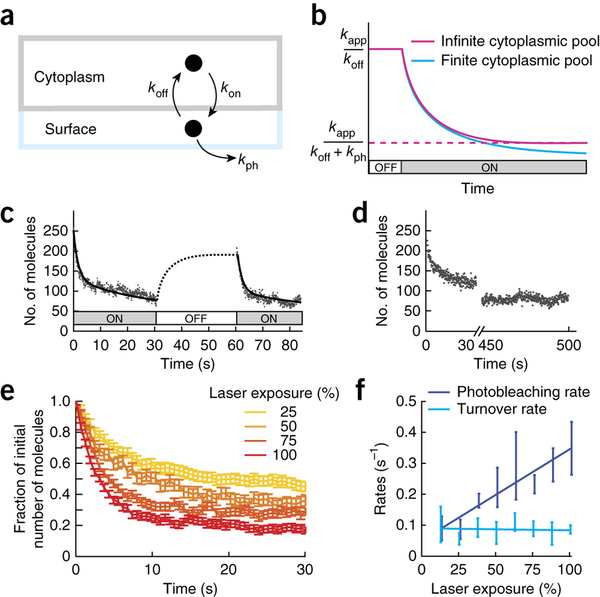
\includegraphics[width=\hsize]{nmeth/nmeth.jpg}
\caption{\label{fig:passive_supp}  Mechanical properties of passive networks.  \textbf{a)} Elastic modulus of networks.  Our measurements closely match prediction of $G_0\sim\mu/l_c$.  \textbf{b)}  Placeholder for inevitably another figure relevant to passive properties.}
\end{figure}
\section{Active Fluid Model Fitting of Cortical Flow Measurement in \textit{C. elegans} embryos}

To ascertain the manner in which active stress and effective viscosity depend upon
actin and myosin densities, I studied cortical flow in the \textit{C. elegans}
single cell embryo during polarity maintenance phase. The single cell \textit{C. elegans}
embryo poses a viable model system wherein to determine how active stress and
effective viscosity depend on constitutive properties of the cytoskeleton. During
the \textit{C. elegans} first division cycle, cell fate determinants and small regulatory
GTPases are segregated between distinct anterior and posterior domains, and these 
asymmetries are actively sustained through regulatory feedback for ~5 minutes 
during the polarity maintenance phase. [11] As displayed in Fig. \ref{fig:measure_flow} this system is 
characterized by a spatially varying distribution of myosin motors 
in the presence of persistent unidirectional cortical flow from the posterior pole 
towards a band of cytoskeletal aggregation near the midline.

In addition to the steady state velocity profile, the \textit{C. elegans} embryo provide a number of
advantages that made these measurements easier. The events of polarization are highly
stereotyped and reproducible, allowing for comparison between experiments. Transgenic strains
expressing fluorescently-tagged variants of myosin-II and F-actin binding proteins (e.g. utrophin and
moesin), allowing for simultaneous visualization of F-actin and myosin by fluorescence microscopy.
In addition, the superficial cortical layer allows for high quality microscopy necessary for the
experiments, and the cell geometry allows simplification to a 2D system. Finally, an important factor
necessary for constraining the theory is a fine level of control over the densities of both actin and
myosin, which can be supplied in the C. elegans embryo by RNAi depletion of nearly any gene
expressed in the germline. [12]



\subsection{Obtaining spatially resolved simultaneous measurement of actin and myosin densities.}

Rationale: Actin and myosin are assumed to be the drivers of cortical flow and their density profiles
and gradients are therefore important variables necessary to parametrize the functions of active stress
and effective viscosity upon which the theory is based.

To obtain the density profile, I used interleaved HILO microscopy timelapses to obtain
simultaneous images of myosin and actin in the C. elegans embryo during the single celled polarity
maintenance phase. Next, I coarse grained the image using image processing blurs or a fixed square
bin so that microscopic inhomogeneity is removed from the measurement. Limiting the analysis to one
dimension improved the measurement quality and made the mathematics simpler so an average
density taken along cross section lines running perpendicular to the embryo AP axis was computed.
The example in Fig. \ref{fig:measure_flow} displays a typical fluorescence image of the myosin localization in the embryo
along with the AP projection axis. The myosin fluorescence profile changes gradually
over the course of five minutes with a period of particular stability lasting roughly two minutes.





\subsection{Obtaining spatially resolved measurement of cortical flow velocities.}
To obtain a flow profile, I analyzed the myosin interframe displacements with
particle image velocimetry (PIV). I averaged a set of contiguous frames from the videos prior to blurring or binning in order to obtain a more clear image and provide a larger flow
displacement between PIV analyzed frames. The PIV algorithm is assumed to maintain a nearly
constant absolute margin of error so maximizing interframe flow distance while still maintaining
consistent results minimizes relative error. I selected a region of interest that remained
consistent throughout all experiments and encompassed the entirety of the dilating and contracting
regions.

The PIV algorithm was an FFT multipass with window deformation and a postprocessing
clean up that rejects and interpolates any velocity with a speed greater than ~3 times the standard
deviation.[13] Only the on axis motion is relevant at this time so the output velocity vectors will be
projected onto a line parallel to the AP axis. This component of the flow velocity was averaged
along the cross sections running perpendicular to the AP axis as before. The diagram below illustrates
a typical PIV flow analysis on the left. On the right, the projection of the flow velocity onto the AP
axis is shown to vary slowly in magnitude over the course of 5 minutes and to maintain the same
overall shape.




\subsection{Using the data to constrain a basic active fluid model}
I compared these measurements to the theoretical predictions by setting up a few nonlinear
functional fits of the velocity, effective viscosity and active stress as a function of myosin
density using a nonlinear least-squares fitting solver with the equation

\begin{equation}
v(x) = C_1 e^{x/l}+C_2 e^{-x/l}+ \int_{a}^{b} \frac{\delta\mu}{\delta x}(e^{(x'-x)/l}+e^{(x-x')/l}
\end{equation}

where $l$ is a length scale of force falloff and the constants $C_1$, $C_2$ are constrained by the boundary conditions at the points $a$ and $b$ in the embryo, $v(a) = v_a$ and $v(b)=v_b$.  See [Bois et al] for more details on this equations derivation.

Data fitting was carried out in MATLAB by passing a starting guess for the fitting coefficients to lsqnonlin along with the function defined above. 


\begin{figure}[h!]
	\centering
	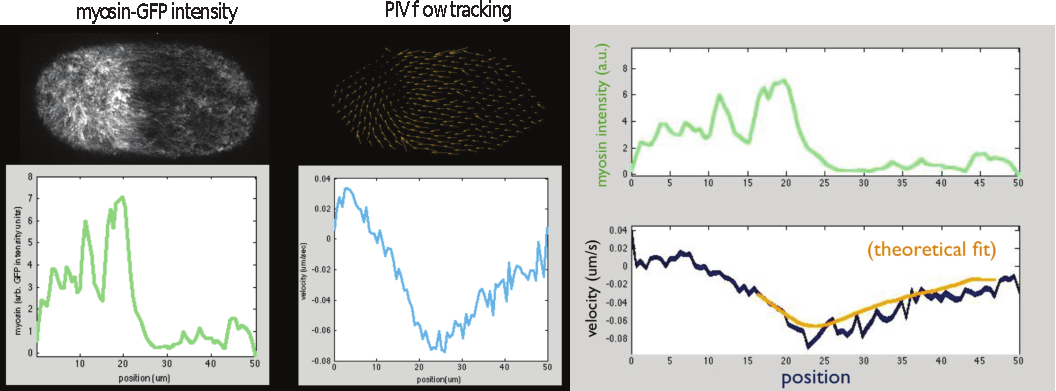
\includegraphics[width=\hsize]{data/prelim_flow.pdf}
	\caption{\label{fig:measure_flow}  Measurement of myosin intensity and flow profile.  These measurements fit a theoretical model of active fluid flow.  }
\end{figure}

The results of this analysis showed that, indeed, an active fluid function akin to that used in [Mayer and Grill] is capable of explaining the observed flow profiles in \textit{C. elegans} embryos.  


\subsection{Disruption of Flow by Myosin Depletion}

The above experiment only sampled a limited region of myosin-actin state space if only analyzed in wild type.
Using only data from this limited region does not uniquely determine the form of the
functions that satisfy the equations of motion. I needed to test outside this range by varying the
concentration of actin and myosin independently in order to adequately constrain the fitted equations
of active stress and effective viscosity.

RNAi depletion is a common practice used to decrease the cellular concentration of endogenously
expressed proteins in C. elegans. By feeding ssRNA containing \textit{E. coli} to mother nematodes, the
mRNA in the nematode germline is progressively silenced and the remaining protein decays away. I used this technique to lower the expression of myosin regulatory light chain kinase (MRCK), which is an upstream regulator of myosin.
Overall
myosin density decreases with a depletion of MRCK.
We assume that the degree of
depletion can be assessed by integrating the myosin density profile over the length of the cell.

Gene depleted embryos were imaged and processed in the exact same
manner as described above for wild type.

\begin{figure}[h!]
	\centering
	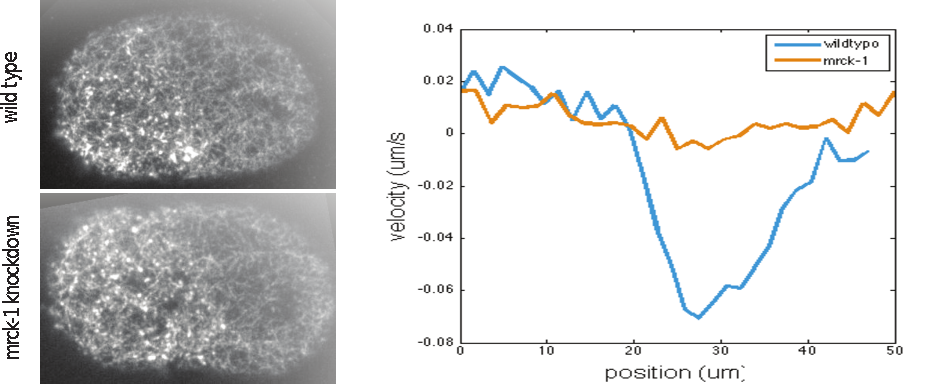
\includegraphics[width=\hsize]{data/flow_mrck_kd.pdf}
	\caption{\label{fig:measure_flow_nomyo}  Measurement of actin distributions and flow profiles for mrck-1 knockdown embryos.  MRCK-1 is an upstream regulator of myosin.  }
\end{figure}

As shown in Fig. \ref{fig:measure_flow_nomyo}, the actin densities were largely unaffected.  Nevertheless, the myosin density (not shown) and flow profile (Fig. \ref{fig:measure_flow_nomyo}, right) were reduced.  Progressive depletion of MRCK also showed a graded response to myosin depletion, indicating that myosin activity imparts internal force in a dose dependent manner.

\section{Stabilization of Filament Turnover with Jasplakinolide Treatment}

Jasplakinolide is a small molecule inhibitor of actin depolymerization.  When treated with jasplakinolide, actin filaments can be stabilized to have very long filament lifetimes.  To study the effect of filament stabilization on cortical flows, Jon Michaux treated embryos with jasplakinolide and imaged the actin cytoskeleton with utrophin::GFP.  The results were striking, and clearly showed that loss of turnover resulted in distrupted flows.  Moreover, in some cases, the treatment didn't just result in a stalling of flows, but also led to a tearing of the cortex followed by further transient contraction.  Nevertheless, all embryos with jasplakinolide treatment eventually stalled and failed to continue with normal polarization and division.

\begin{figure}[h!]
	\centering
	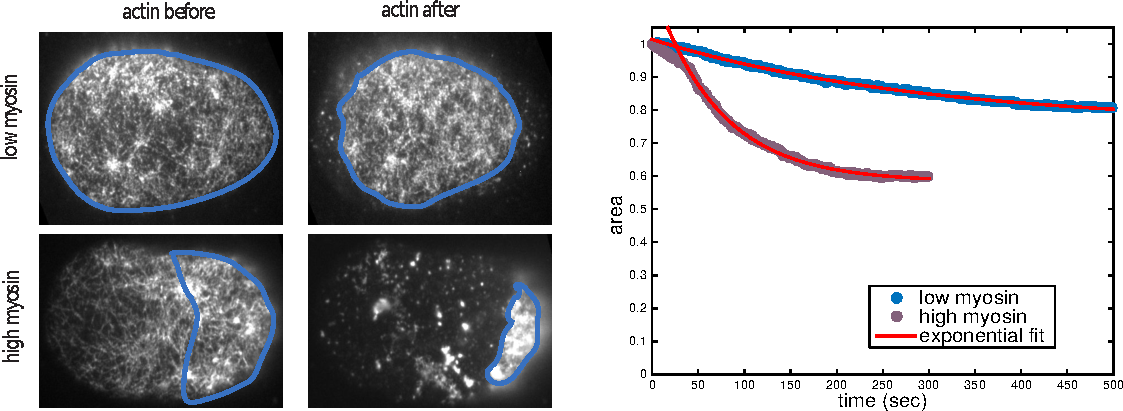
\includegraphics[width=\hsize]{data/jasp_flow_stop.pdf}
	\caption{\label{fig:jasp_flow_stop}    }
\end{figure}

I made an attempt to quantify the degree of contraction possible in jasplakinolide treated embryos using hand tracking of fiducial markers in Jon's videos.  As can be seen in Fig. \ref{fig:jasp_flow_stop}, whether the cortex stalled or tore, the resulting strain asymptotically approached some limiting strain.  This is in sharp contrast to the persistent strains ($\gamma>1$) possible in the steady state flows found when turnover is present.

\chapter{Modeling 2D active networks with recycling}
Our goal was to construct a minimal model that is detailed enough to capture essential microscopic features of cross-linked actomyosin networks (actin filaments with asymmetric compliance, dynamic cross-links, active motors and and continuous filament turnover), but simple enough to explore, systematically, how these microscopic features control macroscopic deformation and flow. We focus on 2D networks because they capture a reasonable approximation of the quasi-2D cortical actomyosin networks that govern flow and deformation in many eukaryotic cells\cite{cellmech_flows, salbreuxbphs}, or the quasi-2D networks studied recently {\em in vitro} \cite{rheo_2D1,rheo_2D2}.




\section{Mathematical Summary of Modeling Methodology}

\subsection{Schematic Overview}
Fig. \ref{fig:model_overview} provides a schematic overview of our model's assumptions. We model each filament as an oriented elastic spring with relaxed length $l_s$. The state of a filament is defined by the positions of its endpoints $\mathbf{x_i}$ and $\mathbf{x_{i+1}}$ marking its (-) and (+) ends respectively. The index i enumerates over all endpoints of all filaments. We refer to the filament connecting endpoint i and i+1 as filament i, and we define $\mathbf{\hat{u_i}}$ to be the unit vector oriented along filament i from endpoint i to endpoint i+1.

\begin{figure}[H]
	\centering
	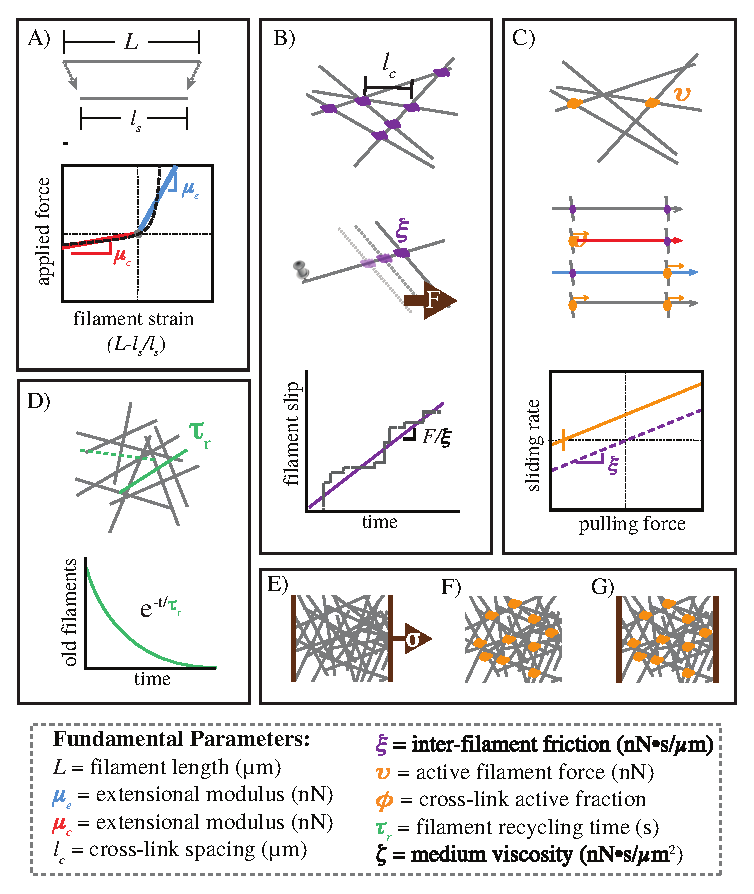
\includegraphics[width=0.8\hsize]{model/figures/Fig1}
	\caption{\label{fig:model_overview} Schematic overview of modeling framework and assumptions. \textbf{A)} Filaments are oriented linear springs that are stiffer in extension than in compression. \textbf{B)} Cross-linking occurs at all filament crossings; we represent cross link resistance as an effective drag, proportional to the relative velocity of the overlapping filaments. \textbf{C)} We represent motor activity as a linear force-velocity relationship with a fixed force at zero velocity directed towards a filament's (-) end. We implement spatial heterogeneity by imposing motor activity at a fixed fraction of filament crossover points, resulting in variation in the magnitudes of compressive vs extensile vs translational forces along individual filament segments. \textbf{D)} Whole filaments disappear at a constant rate; new filaments appear with random positions and orientations at the constant rate per unit area, such that entire network refreshes on a characteristic timescale $\tau_r$. \textbf{e-g)} Three different simulation scenarios: \textbf{E)} Passive response to uniaxial stress, \textbf{F)} Free contraction of an active network and \textbf{G)} Isometric contraction against a fixed boundary. }
\end{figure}

\subsection{Asymmetric filament compliance}
We assume (Fig. \ref{fig:model_overview}A) that local deformation of filament  i gives rise to an elastic force:

\begin{equation}
\label{eqn:spring}
\mathbf{F^{\mu}_{i,i+1}} = \mu \gamma_{i}  \mathbf{\hat{u_i}}
\end{equation}


where $ \gamma_{i} = (|\mathbf{x_{i-1}}-\mathbf{x_i}|-l_s)/l_s$ is the strain on filament i, and the elastic modulus  $\mu$ is a composite quantity that represents both filament and cross-linker compliance as in the effective medium theory of Broederz and colleagues \cite{theo_crosslinknonlinear}.  To model asymmetric filament compliance, we set $\mu = \mu_e$ if the strain is positive (extension), and $\mu = \mu_c$ if the strain is negative (compression). The total elastic force on a filament endpoint $\mathbf{i}$ can be written as:

\begin{equation}
\label{eqn:internal}
\mathbf{F^{elas}_i} =  \mathbf{F^{\mu}_{i,i+1}} - \mathbf{F^{\mu}_{i-1,i}} 
\end{equation}

In the limit of highly rigid cross-links and flexible filaments, our model approaches the pure semi-flexible filament models of \cite{theo_hlm,theo_hlm2}. In the opposite limit (nearly rigid filaments and highly flexible cross links), our model approaches that of \cite{theo_crosslinknonlinear} in small strain regimes before any nonlinear cross link stiffening. 

\subsection{Drag-like coupling between overlapping filaments}
\label{exp_drag}
Previous models represent cross-linkers as elastic connections between pairs of points on neighboring filaments that appear and disappear with either fixed or force-dependent probabilities \cite{model_taeyoon,theo_crosslinknonlinear}.  Here, we introduce a coarse-grained representation of crosslink dynamics by introducing an effective drag force that couples every pair of overlapping filaments, and which represents a molecular friction arising from the time-averaged contributions of many individual transient crosslinks (Fig. \ref{fig:model_overview}B). This coarse-grained approximation has been shown to be adequate in the case of ionic cross-linking of actin\cite{mol_fric,theo_hydroish2}, and has been used to justify simple force-velocity curves for myosin bound filaments in other contexts \cite{theo_frictionShila}. 

To implement coupling through effective drag, for any pair of overlapping filaments j and k, we write the drag force on filament j as:

\begin{equation}
\label{eqn:drag force}
\mathbf{F^{\xi}_{j,k}} = -\xi  (\mathbf{v_{j}}-\mathbf{v_{k}}) 
\end{equation}

where $\xi$ is the drag coefficient and $\mathbf{v_{j}}$, $\mathbf{v_{k}}$ are the average velocities of filaments j and k. We apportion this drag force to the two endpoints ( j, j+1) of filament j as follows: If $\mathbf{x_{j,k}}$ is the position of the filament overlap, then we assign $(1 - \mathbf{\lambda_{j,k}}) \mathbf{F^{\xi}_{j,k}}$ to endpoint j and $\mathbf{\lambda_{j,k}} \mathbf{F^{\xi}_{j,k}}$ to endpoint j+1, where $\mathbf{\lambda_{j,k}} = |\mathbf{x_{j,k}}-\mathbf{x_j}|/|\mathbf{x_{j+1}}-\mathbf{x_j}|$.

The total crosslink coupling force on endpoint i due to overlaps along filament i and i-1 can then be written:

\begin{equation}
\label{eqn: total drag couple}
\mathbf{F^{xl}_{i}} = \sum_j (1 - \mathbf{\lambda_{i,j}}) \mathbf{F^{\xi}_{i,j}} + \sum_k \mathbf{\lambda_{i-1,k}} \mathbf{F^{\xi}_{i-1,k}}
\end{equation}

where the sums are taken over all filaments j and k that overlap with filaments i and i-1 respectively.  

This model assumes a linear relation between the drag force and the velocity difference between attached filaments.   Although non-linearities can arise through force dependent detachment kinetics and/or non-linear force extension of cross-links, we assume here that these non-linear effects are of second or higher order. 

\subsection{Active coupling for motor driven filament interactions}

To add motor activity at the point of overlap between two filaments j and k ; for each filament in the pair, we impose an additional force of magnitude $\upsilon$, directed towards its (-) end (Fig. \ref{fig:model_overview}C):

\begin{equation}
\label{eqn:directedmotorforce}
\mathbf{F^{\upsilon}_{i}}=-\upsilon \mathbf{\hat{u_i}}
\end{equation}

and we impose an equal and opposite force on its overlapping partner.  We distribute these forces to filament endpoints as described above for crosslink coupling forces.  Thus, the total force on endpoint i due to motor activity can be written as:

\begin{equation}
\label{eqn:active}
\mathbf{F^{motor}_{i}} = \upsilon \sum_j (1 - \mathbf{\lambda_{i,j}}) \left (\mathbf{\hat{u_{i}}} - \mathbf{\hat{u_j}} \right ) q_{i,j}
+  \upsilon \sum_k (\mathbf{\lambda_{i-1,k}}) \left (\mathbf{\hat{u_{i-1}}} - \mathbf{\hat{u_k}} \right ) q_{i-1,k} 
\end{equation}


where j and k enumerate over all filaments that overlap with filaments i and i-1 respectively, and $q_{j,k}$ equals 0 or 1 depending on whether there is an ``active'' motor at this location. To model dispersion of motor activity, we set $q_{i,j}=1$  on a randomly selected subset of filament overlaps, such that $\bar{q}=\phi$, where $\bar{q}$ indicates the mean of $q$ (Fig. \ref{fig:model_overview}C).

\subsection{Equations of motion}

To write the full equation of motion for a network of actively and passively coupled elastic filaments, we assume the low Reynold's number limit in which inertial forces can be neglected, and we equate the sum of all forces acting on each filament endpoint to zero to obtain:

\begin{equation}
\label{eqn:syst3}
0=-l_s\zeta\mathbf{ v_i} -\mathbf{F^{xl}_i}+ \mathbf{F^{elas}_i}+\mathbf{F^{motor}_i} 
\end{equation}

where the first term represents the hydrodynamic drag on the half-filament adjoining endpoint i with respect to motion against the surrounding fluid, and $\zeta$ is the drag coefficient.

\subsection{2D network formation}

We used a mikado model approach \cite{Unterberger2014} to initialize a minimal network of overlapping unstressed linear filaments in a rectangular 2D domain. We generate individual filaments by laying down straight lines, of length L, with random position and orientation. We define the density using the average distance between cross-links along a filament, $l_c$. A simple geometrical argument can then be used to derive the number of filaments filling a domain as a function of $L$ and $l_c$ \cite{theo_hlm}.  Here, we use the approximation that the number of filaments needed to tile a rectangular domain of size $D_x \times D_y$  is $2D_xD_y/Ll_c$, and that the length density is therefore simply, $2/l_c$. 

\subsection{Modeling filament turnover}

In living cells, actin filament assembly is governed by multiple factors that control filament nucleation, branching and elongation. Likewise filament disassembly is governed by multiple factors that promote filament severing and monomer dissociation at filament ends. Here, we implement a very simple model for filament turnover in which entire filaments appear with a fixed rate per unit area, $k_{app}$ and disappear at a rate $k_{diss}\rho$, where $\rho$ is a filament density (Fig. \ref{fig:model_overview}D). With this assumption, in the absence of network deformation, the density of filaments will equilibrate to a steady state density, $k_{app}/k_{diss}$, with time constant $\tau_r = 1/k_{diss}$.   In deforming networks, the density will be set by a competition between strain thinning ($\gamma>0$) or thickening ($\gamma<0$), and density equilibration via turnover. To implement this model, at fixed time intervals $\tau_s < 0.01\cdot\tau_r$ (i.e. 1\% of the equilibration time), we selected a fraction, $\tau_s/\tau_r$, of existing filaments (i.e. less than 1\% of the total filaments) for degradation. We then generated a fixed number of new unstrained filaments $k_{app}\tau_sD_xD_y$ at random positions and orientations within the original domain.   We refer to $k_{diss}=1/\tau_r$ as the turnover rate, and to $\tau_r$ as the turnover time.


\subsection{Simulation methods}

Further details regarding our simulation approach and references to our code can be found in the Supplementary Information (\nameref{S1_Text} A.1). Briefly, equations 1-7 define a coupled system of ordinary differential equations that can be written in the form:

\begin{equation}
\mathbf{A \cdot \dot x} = \mathbf{f(x)}
\end{equation}

where $\mathbf{x}$ is a vector of filament endpoint positions, $\mathbf{\dot{x}}$ the endpoint velocities, $\mathbf{A }$ is a matrix with constant coefficients that represent crosslink coupling forces between overlapping filaments, and $\mathbf{f(x)}$ represents the active (motor) and elastic forces on filament endpoints. We smoothed all filament interactions, force fields, and constraints linearly over small regions such that the equations contained no sharp discontinuities. We numerically integrate this system of equations to find the time evolution of the positions of all filament endpoints. We generate a network of filaments with random positions and orientations as described above within a domain of size $D_x$ by $D_y$.  For all simulations, we imposed periodic boundaries in the y-dimension. To impose an extensional stress, we constrained all filament endpoints within a fixed distance $0.05\cdot D_x$ from the left edge of the domain to be non-moving, then we imposed a rightwards force on all endpoints within a distance $0.05\cdot D_x$ from the right edge of the domain.   To simulate free contraction, we removed all constraints at domain boundaries; to assess buildup and maintenance of contractile stress under isometric conditions, we used periodic boundary conditions in both $x$ and $y$ dimensions.

We measured the local velocity of the network at different positions along the axis of deformation as the mean velocity of all filaments intersecting that position; we measured the internal network stress at each axial position by summing the axial component of the tensions on all filaments intersecting that position, and dividing by network height; finally, we measured network strain rate as the average of all filament velocities divided by their positions.

We assigned biological plausible reference values for all parameters (See Table \ref{table:para}).  For individual analyses, we sampled the ranges of parameter values around these reference values shown in \nameref{S1_Table}.

\begin{table}[h]
	\centering
	\caption{Simulation parameters with reference values}
	\label{table:para}
	\begin{tabular}{|c|c|c|c|c|}
		\hline
		{\bf Parameter}             & {\bf Symbol} & {\bf Reference Value}          \\ \hline
		extensional modulus         & $\mu_e$        & $1 nN $                                               \\
		compressional modulus             & $\mu_c$     & $ 0.01 nN $                           \\
		cross-link drag coefficient & $\xi$      & $unknown $              \\
		solvent drag coefficient     & $\zeta$        & $0.0005 \frac{nN s}{\mu m^2} $      \\
		filament length             & L            & $5 \mu m$                                          \\
		cross-link spacing          & $l_c$        & $0.5 \mu m$                                         \\
		active filament force          & $\upsilon$        & $0.1 nN$                                         \\
		active cross-link fraction          & $\phi$        & $0.1<0.9$                                         \\
		domain size                 & $D_x\times D_y$            & $20\times 50 \mu m$                                 \\ \hline
	\end{tabular}
\end{table}


\section{Practical Implementation of Model Framework}

Although the prior description is useful for communicating the mathematical principles underlying my modeling framework, I also want to provide a practical explanation of the logic of the code structure.  This will help to clarify the implementation details that may be ambiguous in the above formulation and make it easier for others to approach and modify my code.

The simulation code is entirely built on top of MATLAB's ode solving functions.  Therefore, at the highest level, the entire simulation framework simply boils down to providing functions to define the ode's left and right hand side, along with the initial conditions for the system.  However, because MATLABs solvers do not allow discontinuities, discontinuous filament recycling events cannot be implemented directly in the ODE.  Effectively, it is necessary to stop the simulation solver at fixed times, reset some subset of filaments, and restart the solver with the new state every time a turnover event happens.


In the following sections, I'll walk through the code's logic in more detail, emphasizing the packages and files that modularly summarize the core functions.  First I will begin with an explanation of the command line interface used to set model parameters and deploy simulations.

To find the \textit{activnet} simulation code, visit:
\begin{verbatim}
https://github.com/wmcfadden/activnet/tree/master/simulation
\end{verbatim}

\subsection{Launching simulations from the command line}



The activnet package includes a function called activnet\_gen.m, which can be used to launch simulations on any MATLAB system.  The following is the documentation of the parameters passed to this function.

\begin{verbatim}
function p = activnet_gen(zet,L,mu,kap,lc,xi,ups,phi,psi,
                          r,sig,Dx,Dy,Df,Dw,ls,lf,tinc,tfin,nonlin)
% generates an active network simulation and prints node positions
% at time steps.  Parameters are defined as follows:
%
%   zet - medium viscosity
%   L - length of the filament
%   mu - compressional modulus of the filament
%   kap - bending modulus of a filament if ls<L
%   lc - average distance between filament overlaps
%   xi - frictional resistance between two overlapping segments
%   ups - motor force at filament overlaps
%   phi - fraction of overlaps that receive a motor force
%   psi - spatial variation in motor force 
%         (if external force applied, psi sets the periodicity of 
%          force application, and psi<0 sets square wave.)
%   r - recycling rate
%   sig - applied stress in the x direction applied at Df*Dx
%         (sig<0 sets stress to be applied in y direction)
%   Dx - x-dimension of domain
%   Dy - y-dimension of domain
%   Df - position at which external force is applied
%        (if Df<0, also position in x dimension where network stops)
%   Dw - width of window in x-dimension where forces are applied
%   ls - length of filament segments
%   lf - length of force falloff at end of filament 
%         (just ensures continuous forces)
%   tinc - time increment to return solutions 
%          (will be decreassed automatically if r is too large)
%   tfin - end time of simulation
%   nonlin - factor by which to make filament stiffer for extension
%            (if nonlin<0, add spacing so filaments dont reach edge)
\end{verbatim}

These parameters will be explained in more detail below, but here I'll provide a brief practical explanation for their use in setting up simulations.  The parameters \texttt{zet}, \texttt{L}, \texttt{mu}, \texttt{kap}, \texttt{lc}, \texttt{xi}, \texttt{ups}, \texttt{phi}, \texttt{r}, \texttt{sig}, \texttt{Dx}, and \texttt{Dy} are defined in the mathematical methods section above as $\zeta$, $L$, $\mu_c$, $\kappa$, $l_c$, $\xi$, $\upsilon$, $\phi$, $1/\tau_r$, $\sigma$, $D_x$, and $D_y$, respectively. The parameter \texttt{nonlin} is used to internally calculate the extensional modulus $\mu_e = \texttt{nonlin} \times \mu_c$ (i.e. if \texttt{mu} is 1 and \texttt{nonlin} is 100, then $\mu_c=1$ and $\mu_e=100$).  The parameter \texttt{psi} is used to generate a spatial gradient in internal activity or temporal periodicity if an external force is applied. The spatial gradient is linear with a maximum at the center of the domain.  The parameter \texttt{Df} defines the fraction along the x-domain where any external stress will be applied (i.e. stress is applied at \texttt{Df}*\texttt{Dx}).

All of these terms are positive by definition so setting certain terms negative is used to trigger certain behavior in the simulation environment:
\begin{itemize}
	\item  Setting $\texttt{mu} < 0$ enables the extensional spring constant to be different than the compressive.
	\item  Setting $\texttt{sig} < 0$ causes the external stress to be applied in the y direction rather than the x direction, resulting in shear stress simulations.
	\item Setting $\texttt{nonlin} < 0$ results in space being added to the edge of the domain so that no filaments intersect with the boundaries of the simulation, allowing the network to undergo unconstrained contraction.
	\item Setting $\texttt{psi} < 0$ results in oscillating positive and negative stresses being applied to the network (as opposed to a sinusoidal pattern regularly).
	\item Setting $\texttt{Df} < 0$ will cause the rightward edge of the initially generated network to end at the location where the force is applied.
\end{itemize}
   
The parameter \texttt{ls} sets the segment size of the filament.  Theoretically this segment size is very small (the size of a single actin monomer perhaps), but for computational reasons this value is set much larger.  The parameters \texttt{Dw} and \texttt{lf} set the regions over which forces will "fall off" for the domain and individual filaments, respectively.  These are just there to ensure there are no discontinuous changes in the ODE equation as filaments move around, and should be set to some smallish number, like $0.05$, but don't affect the results too much overall.  Finally, \texttt{tfin} and \texttt{tinc} set the end time of the simulation and the timesteps at which to print results, respectively.  The program will automatically shrink \texttt{tinc} if the recycling rate, \texttt{r}, is large enough that manual position updates must occur on timescales smaller than \texttt{tinc}.


To run a simulation with an external stress the following code could be used.

\begin{verbatim}
activnet_gen(0.001, 1, -0.01,  0,  0.8, 10, 0, 0, 0, 
             0, -0.002, 20, 4, -0.33, 0.05, 1, 0.025, 1, 10000, 100)
\end{verbatim}

To run a simulation with internal filament activity the following code could be used.

\begin{verbatim}
activnet_gen(0.001, 5, -0.01,  0,  0.3, 10, 0.1, 0.25, 0, 
             0.001, 0, 25, 25, 0.5, 0.05, 5, 0.025, 1, 10000, -100)
\end{verbatim}

Both of these have nonlinear filament extension because the third argument (\texttt{mu}) is less than 0.  The results will be printed to the MATLAB console.

The currently deployed package can also be used to launch simulations on any linux system with MATLAB 2014b or the MATLAB 2014b Compiler Runtime installed (you will need to have a \$MATLAB environment variable enabled.  Please contact your sysadmin.).  In addition, the package can be recompiled on any system running MATLAB to create a new deployment that will run on the compiled MATLAB version and operating system (see the README.txt file for more information about deployment).  

\begin{verbatim}
./run_activnet_gen.sh $MATLAB 0.001 1 -0.01  0  0.8 10 0 0 0 0 
         -0.002 20 4 -0.33 0.05 1 0.025 1 10000 100 > output.file
\end{verbatim}




\subsection{Package structure of activnet}

To understand the high-level overview of this code, you can analyze the basic package structure and the small number of important top level packages.

\begin{itemize}
	\item  activnet\_gen.m: topmost wrapping function to call for running simulations; confirms input, generates initial conditions, and calls activnet.m.
	\item  activnet.m: Chooses between which ODE implementation to run; stops ODE solver execution to perform filament recycling.
	\item odes folder: Contains all the ODE computation internals.
	\item helpers folder: Some additional functions written to perform line intersection tests.
	\item analysis folder: All the code used to generate the figures in the accompanying publication.
\end{itemize}


Note: the rest of this documentation is most useful if one is looking over the internals of the code.  Trying to understand this without working with the code is probably not very useful.

\subsection{ODE Wrapper functions }

As mentioned above, the initialization and launch of the simulation takes place using the function activnet\_gen.m.  This function is quite simple. It just ensures proper input parameters, builds a randomized network of filaments, prints the network node positions, and then calls the function activnet.m to compute the simulation results.  From there, activnet.m takes care of pausing solvers to update filament position for recycling as well as choosing between solvers depending on the type of problem being solved.  

\subsubsection{Generating Initial Conditions}

Before an ODE solver can be called, one needs to set up the initial conditions of the network.  Every solver implementation in MATLAB operates on 1D vectors where every element represents a variable to be integrated.  Therefore, the data structure for this model is going to need to be set up to be encoded as a 1D vector of numbers.  Because the model framework is based around the 2D position of points, I will continually be shifting between the 1D vector, \texttt{z} and the 2D vector \texttt{p} using the following transformations.

\begin{verbatim}
p = reshape(z0,[],2);  % z -> p
z0 = reshape(p,1,[]);  % z -> p
\end{verbatim}

To select the number of filaments, $\texttt{N}$, to generate using the input parameters, we use the approximating formula $\texttt{N} \approx \texttt{floor(2*Dx*Dy/lc/L)}$.  This formula is derived from the tiling of a $Dx \times Dy$ domain with lines of length $L$ and spacings between lines $lc$.  This diverges from the exact number of filaments needed when $L/lc$ is small, but we ignore this discrepancy because we mostly operate in the regime where $L/lc>10$.

We therefore begin by creating an initial set of filament segment endpoints \texttt{p}, where we want to have \texttt{N} total filaments each with \texttt{ncnt} segment endpoints.  We do this by selecting a random starting point in our domain (\texttt{Dx} by \texttt{Dy}) with random orientation (\texttt{thet}).

\begin{verbatim}
 p = zeros(N*ncnt,2);   %initialize all endpoints to 0
 for i=1:N
	 p((i-1)*ncnt+1,:) = [Dp*Dx*rand Dy*rand]; %random starting location
	 thet = rand*2*pi;                         %random direction
	 for j = 2:ncnt            % iterate through remaining segments to add endpoints
		 p((i-1)*ncnt+j,:) = p((i-1)*ncnt+j-1,:)+L/(ncnt-1.0)*[cos(thet) sin(thet)];
	 end
 end
\end{verbatim}

In most cases, the network should be assembled such that the domain is filled entirely in the y dimension ($y=0$ and $y=Dy$) and filled to the left edge ($x=0$) and up to the position $x=Dp*Dx$ in the in the x-dimension.  However, in the case that the parameter \texttt{nonlin} is less than 0, we set the initial conditions such that there is an empty space of size $0.2 Dx$ and $0.2 Dy$ at the x and y boundaries.  

To keep our density the same we should adjust our calculation of $N$ above, however, in the current implementation this adjustment is not made. This is a known bug that was corrected for after-the-fact in the publication by multiplication of $l_c$ by a constant factor depending on the simulation setup. 


\subsubsection{Choosing between active and driven simulations }

During development I noticed that there were some cases where I could skip certain sections of the computation to speed up integration of the ODEs.  In particular, when there is no internal forces generated by filament activity, the right hand side of the differential equation is easier to compute (see below).  Therefore, in any situation where internal activity is set to 0, we use the more efficient code.  The activnet.m code makes this decision by determining if there is "pulling" of filaments rather than internal force generation.  

\begin{verbatim}
pull = (isempty(nu)&&sig~=0) 
\end{verbatim}

In this case it runs a different pair of functions to compute the ODE right hand side and mass matrix (see below).

\subsubsection{Implementing Filament Recycling }

The core function of activnet.m is to serve as a wrapper for the ODE solvers mentioned above and described in greater detail below.  However, since the ODE solvers won't allow discontinuous changes to the positions of nodes, activnet.m must also carryout the task of stitching together smaller simulations and manually updating positions in between.  The code in activnet.m implements a repeated loop with calls to the underlying ode solvers. If $r>0$, a solver computes the integral between two adjacent time points in the vector of all time points to evaluate, $tt$. Then the positions are updated and the solver is used to evaluate integral for the next time interval. Logic implemented in activnet\_gen.m ensures that the timesteps are selected small enough so that there will not be too many filaments disappearing at once.

The following code chunk implements the position update for a randomly selected subset of nodes whenever the recycling rate, r, is greater than 0.  The logic implemented in activnet\_gen.m ensures that the timesteps are not so large that more than 5\% of filaments will be undergoing a discontinuous jump at any one time (i.e $r*istep*tinc <0.05$).

\begin{verbatim}
				% % select random indices
i = randi(N,floor(r*istep*tinc*N)+(rand<mod(r*istep*tinc*N,1)),1); 
				% % reset the position of the first segment endpoint
p((i-1)*ncnt+1,:) = [Dp*Dx*rand(size(i)) Dy*rand(size(i))];
				% % pick random orientation for each filament
thet = rand(size(i))*2*pi;
for j = 2:ncnt  % % iterate over rest of endpoints
  p((i-1)*ncnt+j,:) = 
			  p((i-1)*ncnt+j-1,:)+L/(ncnt-1.0)*[cos(thet) sin(thet)];
end

\end{verbatim}


\subsection{Overview of Numerical Integration Implementations}
As mentioned above, the solution is numerically integrated using MATLAB's built-in ODE solvers.  The ODE equation is the low-Reynolds limit of Newton's equation of motion for all the filaments.  So to implement, I simply supply an ode solver with a function to compute the right hand side of a system of differential equations ($\mathbf{f(x)}$) along with a function to compute the mass matrix ($\mathbf{A}$) that connects the derivatives on the left hand side of the ODE system.

\begin{equation}
\mathbf{A \cdot \dot x} = \mathbf{f(x)}
\end{equation}

With those two matrices, the system of differential equations can then be integrated to the desired level of precision by one of MATLABs implicit ode solvers (e.g. ode15s or ode23).  In that equation, $\mathbf{x}$ simply represents the positions of filament endpoints (nodes).  Therefore $\mathbf{\dot{x}}$ is just a way to represent the velocity of every endpoint.  

The right hand side represents the forces (external or internal) driving the motion of the filaments.  The mass matrix $\mathbf{A}$ represents the coupling of filaments to each other (off diagonal elements) and to the solvent in which they are embedded (diagonal elements).  Once those are provided, MATLAB's solvers take care of the integration (see MATLAB ode solver documentation for more info).


\subsubsection{Right hand sides: \textit{activnet\_act\_ode.m vs. activenet\_pull\_ode.m}}

The right hand side of the equation constitutes all the non-viscous forces in the simulation.  The most important and fundamental forces are those of the intrafilament spring mechanics.  In these simulations, filaments are represented by chains of filament segments that act as springs with particular properties.  As described above, each segment has a compressive (\texttt{mu}) and extensional ($\texttt{mu}\times\texttt{nonlin}$) spring constant that governs the motion between endpoints along the length of each filament.  There is also a bending spring constant (\texttt{kap}) which effectively tries to straighten adjoining segments if they are not already colinear.  The internal mechanical forces of all filaments in the simulation is represented in the following code snippet.

\begin{verbatim}
%% compute intrafilament forces    
l0 = L/(ncnt-1);           % length of segment
dp = zeros(size(p));
for n=1:ncnt:length(p)
  va_orth=[0 0];
  va = [0 0];
  la = 0;
  for i=0:ncnt-2
			  % % custom subtraction minding boundaries
    vb = mydiff(p(n+i,:),p(n+i+1,:),Dx,Dy); 
    lb = sqrt(vb*vb');
    gam = (lb-l0)/l0;      % extension of the segment
    f = mu*vb/lb*gam;      % longitudinal spring force
    if(mu<0)               % allow nonlinearity
      f = -f*(1+(muN-1)*double(gam>0));
    end
    dp(n+i,:) = dp(n+i,:) + f;
    dp(n+i+1,:) = dp(n+i+1,:) - f;
    
    % % below is for bending stiffness
    
    vb_orth = [-vb(2) vb(1)];
    if(i>0)
      if(va_orth*vb'>0)
        va_orth = -va_orth;
      end
      if(vb_orth*va'<0)
        vb_orth = -vb_orth;
      end
      tor = kap/l0^2*acos(max(min(va*vb'/la/lb,1),0));
      dp(n+i-1,:)=dp(n+i-1,:)+tor*va_orth/la;
      dp(n+i,:)=dp(n+i,:)-tor*va_orth/la;
      dp(n+i+1,:)=dp(n+i+1,:)+tor*vb_orth/lb;
      dp(n+i,:)=dp(n+i,:)-tor*vb_orth/lb;
    end
    va = vb;
    va_orth = vb_orth;
    la = lb;
  end
end
\end{verbatim}

The code loops over every \texttt{ncnt} nodes, which constitute the nodes of a single filament.  Next the code loops through each node of the individual filament.  First, the code evaluates the extensional force on each node given by \texttt{f = mu*vb/lb*gam} with the modification that if \texttt{mu}$<0$ and \texttt{gam}$>0$, the force constant is modified to incorporate the nonlinear extensional stiffness.  Next, the code evaluates the bending forces for adjacent segments that are not aligned using 

\texttt{tor = kap/l0\^2*acos(max(min(va*vb'/la/lb,1),0))}. 

 The \texttt{max(min(...))} is used simply to ensure that there are no aberrantly large values due to errors in evaluation of \texttt{acos} with arguments very slightly greater than 1 or less than 0.   The two vectors \texttt{va\_orth} and \texttt{vb\_orth} are calculated to direct the force orthogonal to the orientation of the filament segment.  Finally, it should be noted that a bending force is generated from both the segment behind and the segment in front of the current node of interest and that the force from these need to be assigned at both the current node and the equal and opposite force assigned at the other end of each filament.

After the basic mechanical properties of the filament are accounted for, we need to add extra forces (otherwise the simulations won't be any more interesting than just a bunch of inert springs).  What we do depends on whether the simulation is meant to represent active motors or a passive network with an external driver.  In the next two sections we cover the specifics of the force equations for both of these cases.

\subsubsection{Active ODE}

For the ODE with internal activity, we need to compute a very different force on each node.  In particular, we have to check for intersections and add forces to filaments that intersect as if they are being pulled on by an active motor at their overlap point.  To do this we will use one of the helper functions described below to return all of our overlapping lines.  After that we will step through all pairs of intersecting lines and add the appropriate force in the appropriate direction.  The following code snippet shows the process with documentation.  

\begin{verbatim}
g = lineSegmentGrid(indL,XY,Dx,Dy,l0);  % find instersecting lines

	% find distance of intersections from endpoints
f = min(1,max(0,(g-lf/2)/(1-lf)));     
for ind=1:size(g,1)
  i = g(ind,3);
  j = g(ind,4);

  vm = mydiff(p(j,:),p(j+1,:),Dx,Dy);
  lm = sqrt(vm*vm');

  edg = 1;   % this will be used to reduce the force 
			 % as it gets closer to the edge of a filament

  if(g(ind,1)<lf)
    edg = edg*g(ind,1)/lf;
  elseif((1-g(ind,1))<lf)
    edg = edg*(1-g(ind,1))/lf;
  end

  if(g(ind,2)<lf)
    edg = edg*g(ind,2)/lf;
  elseif((1-g(ind,2))<lf)
    edg = edg*(1-g(ind,2))/lf;
  end
  
  mul = 1;   % this will be used to modulate the force if
             % psi says there should be a spatial gradient
  
  if(psi>0)
    mul = double(g(ind,5)>=psi*abs(-Dx*Df));
  end
  
  tnu = nu(ceil(i/ncnt),ceil(j/ncnt))*mul;  % variation in 
											% filament force (phi)
  
  dp(i:i+1,:) = dp(i:i+1,:) + edg*tnu/lm*[vm*(1-f(ind,1));vm*f(ind,1)];
  dp(j:j+1,:) = dp(j:j+1,:) - edg*tnu/lm*[vm*(1-f(ind,2));vm*f(ind,2)];

end
\end{verbatim}

The last line shows the net force that is added to both pairs of nodes that are intersecting (\texttt{i:i+1} and \texttt{j:j+1}) with one positive and the other negative to conserve the net force to be 0.  The term \texttt{f} is the distance of the overlap point between the two nearest node locations, and is used to set how much force is applied to the first vs second node.  For each iteration of the loop, the force is calculated for the \texttt{j:j+1} filament, and each interaction is stepped through twice (once with each filament in the \texttt{j:j+1} role).  The vm calculation determines the direction in which the forces will be applied.  The terms \texttt{edg} and \texttt{tnu} simply modify the applied force by scalar quantities based on closeness to the end of the filament and spatial variation in motor force intensity.



\subsubsection{Pulling ODE}

For the case of the system with an external stress, we will need to add forces at the desired location of stress, and we will need to constrain the filaments located at the edge of the domain.  The following two code snippets show these two behaviors.


\begin{verbatim}
%% add external force at centerline
if(psi>0)
val = sig*sin(psi*t);
elseif(psi<0)
val = sig*round(mod(0.5+-psi*t,1)).*(round(mod(0.55+-psi*t/2,1))-0.5)*2;
else
val = sig;
end

subp = p(:,1)>(Df-Dw)*Dx&p(:,1)<(Df+Dw)*Dx;
ff = 1-abs(p(subp,1)-Df*Dx)/Dw/Dx;
if(sig<0)
  dp(subp,1)=dp(subp,1) - Dy*val.*ff/sum(ff);
else
  dp(subp,2)=dp(subp,2) - Dy*val.*ff/sum(ff);
end
\end{verbatim}

The top section of this code calculates stress that should be applied and sets that as \texttt{val}.  If \texttt{psi} is nonzero then we are looking to have a temporally varying applied stress.  If $\texttt{psi}>0$, then we want a sinusoidally varying stress with frequency psi.  If $\texttt{psi}<0$, then we want a square wave with frequency psi.  The max stress in each case is still \texttt{sig}.

The bottom section selects the nodes that will have force added to them in \texttt{subp}.  The force to be applied to each node is not equally distributed, but instead, \texttt{ff} sets the fraction of force to be proportional to the distance to the center of the region of applied stress (set by the width \texttt{Dw}).  This distribution function is normalized so that the total amount of force is equal to the amount of force needed to set the stress to \texttt{val} (i.e. $F_{total} = \texttt{val} \times \texttt{Dy}$).  Finally the force is applied in the x direction or the y direction based on whether \texttt{sig} is greater or less than 0.


\begin{verbatim}
% % constrain edges
subp = p(:,1)<Dw*Dx;
dp(subp,:)=dp(subp,:).*repmat(4*p(subp,1)/Dw/Dx-3,1,2);

subp = p(:,1)>Dx*(1-Dw);
dp(subp,:)=dp(subp,:).*repmat(4*abs(p(subp,1)-Dx)/Dw/Dx-3,1,2);

subp = p(:,1)<3*Dx/4*Dw|p(:,1)>Dx-3*Dx/4*Dw;
dp(subp,:)=0;
\end{verbatim}

This last segment merely constrains the force at the far left and right edges of the domain to be 0 (within $0.75 \texttt{Dw}\times\texttt{Dx}$ from each edge).  There is a linear transition to \texttt{dp=0} in the remaining 25\% of the region.

It should be noted that in the "pulling" simulations, there is no need to compute the intersection of filaments.  This means that there are far fewer computations than in the active case.   I wrote two separate functions for each of the different cases simply to avoid having to perform redundant checks on the cases repeatedly (i.e. the choice is made once in the outer wrapping functions rather than having to repeatedly make the choice for which code to run on each iteration of the solver).

\subsection{Left hand side: Understanding the mass matrix}

It can be somewhat difficult to understand how a mass matrix works in a system of coupled differential equations.  In this particular use-case, I'm using a mass matrix to delineate how we couple the filament velocities together.  To understand the logic of coupling filaments together by their velocities it might be helpful to look at a simple example.  Imagine that you have a single particle in some one-dimensional fluid with viscosity, $\zeta$, and with a force, $F$, acting on it.  Assuming low Reynolds limit so there is no acceleration of the particle, the equation of motion would look like the following.

\begin{equation}
\zeta\dot{x}=F
\end{equation}

Now assume you have two particles in that fluid, but (for now) we assume the particles can't interact in any way.  Therefore, we can express the equation of motion for both particles pretty simply with the following equation.

\begin{equation}
\zeta\mathbf{\dot{x}}=\mathbf{F}
\end{equation}

Obviously, all we did was replace the scalars with vectors.  To make things a little neater we could replace the scalar $\zeta$ with a so called "mass matrix" that would simply look like the following matrix.

\begin{equation}
\mathbf{A} = \begin{bmatrix} \zeta & 0 \\ 0 & \zeta \end{bmatrix}
\end{equation}

Now, if we had some drag-like coupling between the velocities of our two particles with a drag coefficient, $\xi$, we could simply add a term to the off diagonal.

\begin{equation}
\mathbf{A} = \begin{bmatrix} \zeta & -\xi \\ -\xi & \zeta \end{bmatrix}
\end{equation}

And carrying out our math we can see that this just gives a frictional coupling between the two particles.

\begin{equation}
\begin{array}{lcl} \zeta v_1 - \xi v_2  & = & F_1 \\ \zeta v_2 - \xi v_1 & = & F_2 \end{array}
\end{equation}

This is the entire logic behind the construction of the activnet\_mass.m function.  After finding which filament segments are overlapping, I simply add off-diagonal terms to the mass matrix that couple the nodes of those filament segments together.

Similar to the previous section, there are computational efficiencies to be gained in computing the mass matrix, $\mathbf{A}$, if the system is being driven externally (as opposed to being driven by internal activity).  

\subsubsection{\textit{activnet\_mass.m vs. activenet\_mass\_sp.m}}
When we are constraining filaments to remain motionless we run into one little problem with our mass matrix formulation as presented thus far.  Essentially, the right hand side of the equation is being set to 0, but the left hand side still has cross terms.  To remedy this, in the case where an external stress is applied, I need to manually decouple filaments that lie along the $x=0$ boundary of the domain.  This is carried out in activenet\_mass\_sp.m, but it is not implemented in activenet\_mass.m because that code only runs in the case where there is internal activity of the filaments and no external constraints.

Additionally, in activenet\_mass\_sp.m, I utilize a sparse matrix because I found in that condition I could get some kind of marginal speedup by using a sparse matrix instead of the full matrix.


\subsection{Line intersection \textit{helper} Functions}
There are a series of helper functions that are called to aid in the calculations of filament intersections.  You can analyze the code directly for more detail but briefly, the lineSegmentIntersect.m implementation manually computes the intersection between all pairs of segments while lineSegmentGrid.m first bins lines into grids before testing intersection just on those in the bin.  I empirically observed a significant improvement in runtime when I moved to lineSegmentGrid even though asymptotically they both perform worst case $O(n^2)$, which I believe is due to the uniformity of the line segment distribution.  It is interesting to note that the classical best-case line scanning algorithm (i.e. sweep line) is $O(nlogn)$.

\subsection{Visualization code}
In the analysis package, I have included some code called netplot\_str.m to aid with visualizing the output of the simulations.  This code opens the output file and an accompanying script file to get the parameters passed to the function.  The code then goes on to render all the lines in a MATLAB plot.  It could be modified easily to render the output in whatever format you may need.  

\chapter{Phases of deformation in filament networks with cross-link slip}
\documentclass[pre,preprint]{revtex4-1}

% preamble:
\usepackage{appendix}
\usepackage{outline}
\usepackage{amsmath}    % need for subequations
\usepackage{graphicx}   % need for figures
\usepackage{verbatim}   % useful for program listings
\usepackage{color}      % use if color is used in text
\usepackage{subfigure}  % use for side-by-side figures
\usepackage{hyperref}   % use for hypertext links, including those to external documents and URLs
\raggedbottom           % don't add extra vertical space
\begin{comment}
\pagestyle{empty}       % use if page numbers not wanted
\end{comment}




\begin{document}

\title{Phases of deformation in filament networks with cross-link slip}
\author{William McFadden, Edwin Munro}
\affiliation{University of Chicago, Institute for Biophysical Dynamics, Chicago, IL 60615}

\date{this day}


\begin{abstract}
Here we combine theoretical and computational approaches to explore mechanisms that govern  long timescale deformation in semi-flexible filament networks with transient cross-links.  We introduce a coarse-grained representation of cross-link dynamics in which cross-linked filaments slip past one another with an effective friction representing the time-averaged contributions of transient elastic cross-links.  For small strains, we obtain a theoretical prediction for the long timescale effective viscosity of the network that depends on network architecture and effective friction coefficient between filaments, and we confirm this prediction using numerical simulations.  We show computationally that network response deviates significantly from purely viscous creep when networks undergo large strains that drive them into anisotropic configurations.  Interestingly, under certain conditions, we find a phase of long-lived sub-linear creep, suggesting that our simple model may account for the long-lived transitional phase between purely elastic and purely viscous rheology as measured in actin biopolymer experiments.  
\end{abstract}



\maketitle


\tableofcontents


















\section{Introduction}

Cross-linked networks of semi-flexible polymers are a class of materials with poorly understood but highly interesting properties.    Early studies of semi-flexible polymer networks reconstituted {\em in vitro} revealed novel, nonlinear rheology, spurring interest from materials scientists\cite{megareview}.  Cross-linked networks of cytoskeletal polymers have been a subject of great interest to biologists  because of their importance as structural components of cells\cite{cellmech_review1,cellmech_review2}.


On shorter timescales, the response of cross-linked polymer networks to applied stress can be well-described theoretically in terms of purely elastic mechanical resistance.  On longer timescales, the network's elastic resistance begins to give way to a viscous relaxation of stored stress, but the mechanisms that govern this viscous relaxation remain poorly understood.   It is important to understand the mechanism behind this long timescale relaxation of cross-linked polymer networks both for understanding their novel material properties as well as understanding how this effect may govern physiologically important cellular processes\cite{cell_rheo}.


For {\em in vitro} reconstitutions, this viscous relaxation is thought to result from transient unbinding and rebinding of intermolecular cross-links\cite{rheo_crosslinksmatter,theo_crosslinkslip1}. However, there is still no clear understanding of how local relaxations of network connectivity would give rise to a global viscous relaxation.  In our work, we wish to expand upon a well-established mechanical picture of cross-linked semi-flexible polymer networks to incorporate slippage of cross-links over longer timescales.  


\subsection{Short Timescale Mechanics of Cross-linked Actin Filament Networks}


Early {\em in vitro}  studies of cross-linked actin filament networks revealed strikingly different elastic behaviors compared to the already well-understood flexible polymer gels \cite{rheo_bench}.  The complexity of these behaviors drove a surge in both experimental and theoretical studies of semi-flexible networks.  For a comprehensive review of this field we recommend \cite{megareview}, but we will shortly repeat some important milestones here.

\subsubsection{Theories of Semi-flexible Filament Networks}
 
Diversity and discrepancy in observations led a drive toward systematic {\em in vitro} experimental explorations of the rheology of cross-linked semi-flexible polymer networks at short timescales.  In studies with rigid irreversibly cross-linked networks, it was found that differences in network structure could lead to remarkably different elastic moduli, suggesting distinct phases of mechanical response \cite{rheo_marge}.  These discoveries in turn begat theoretical work on the basic implications of the semi-flexible nature of filaments on network mechanics.  

Prior work on the basic physics of individual semi-flexible polymers \cite{mol_wlc,theo_doi_ed}, and comprehensive theories of semi-flexible filament solutions, \cite{theo_morse} laid a groundwork for theoretical considerations of cross-linked networks. Beginning with the so-called "mikado model" descriptions\cite{theo_hlm,theo_hlm2}, it was determined that there should exist a minimum rigidity percolation threshold, and that the connectivity of the network determined whether the mechanical response was dominated by non-affine bending or affine stretching of filaments.   Continuing to more explicit theories\cite{theo_best}, the mechanics of rigidly cross-linked networks were shown to be well-described in terms of purely elastic stretching of filaments between cross-linked points.  

\subsubsection{Incorporating Effects of Cross-link Compliance}

Despite the success of the theory for rigid cross-links, early studies showed that surprising qualitative differences in mechanical response could be traced to differences in the chosen cross-linker\cite{rheo_crosslinkcompare,rheo_crosslinkreview}.  In addition, many studies using more compliant cross-linkers showed that cross-linker compliance could give rise to different nonlinear rheological properties on short timescales\cite{rheo_crosslink_nonlin1,rheo_crosslink_nonlin2,rheo_crosslink_nonlin3,rheo_crosslink_notactin}. Making matters even more complicated, ongoing research has begun to uncover added complexity from more highly complex issues such as filament bundling\cite{theo_crosslinkslip2,model_massive}and the effects of active cross-linking by molecular motors\cite{rheo_active}.

While theorists have built a number of largely successful models that help characterize different aspects of the cross-link dominated response\cite{theo_nonaffine2,theo_floppy,theo_crosslinknonlinear}, the diversity of behaviors of these networks makes a precise yet general theory more difficult.

\subsection{Long Timescale Stress Relaxation from Transient Cross-link Unbinding}

At long timescales, the purely elastic behavior of cross-linked networks gives way to fluid-like stress relaxation. Additionally, fluid-like flows have been observed in a number of cellular processes\cite{cellmech_flows,cellmech_flows2,cellmech_flows3,rheo_fluid,rheo_fluid2,cell_rheo_exp}.  In {\em in vitro} studies, long timescale creep behaviors are thought to arise predominantly from the transient nature of filament binding for most biologically relevant cross-linkers\cite{rheo_crosslinkslip1,rheo_crosslinkslip2,rheo_crosslinkslip3,rheo_nonaffine}.  While the importance of cross-link dynamics in determining the mechanical response of semi-flexible polymer networks has been known for at least 20 years\cite{rheo_crosslinksmatter}, there is still a gap in our understanding of how microscopic cross-link unbinding relates to viscous flows. 

\subsubsection{Models of Stress Relaxation with Transient Cross-links}

The dependence of network rheology on cross-link unbinding is an active subject of theoretical research\cite{theo_crosslinkslip2}.  

Several theoretical methods have addressed cross-link binding and unbinding directly \cite{theo_crosslinkslip1,theo_crosslinkslip2} in analytical approaches that allowed well-constrained fits for specific cross-linkers.  These theories have therefore focused conceptually at the level of the cross-linked filament and were extended analytically to macroscopic networks.  In another approach, modelers have taken cross-links as extended springlike structures \cite{model_taeyoon} that are able to bind and unbind in simulated filament networks. Finally, other more ambitious simulations have even sought to interrogate the effects of cross-link unbinding in combination with the more complex mechanics of filament bundles\cite{rheo_crosslinkslip2,theo_crosslinkslip3}.

Ultimately, the complexity of the many theoretical approaches that have been applied to this problem have made it difficult to distinguish what, if any, core physical mechanisms may be sufficient to explain the observed forms of stress relaxation.  We believe that serious qualitative understanding can be generated by focusing on some of the common elements exhibited in the aforementioned literature.

\subsubsection{Novelty of Cross-link Slip Approach}

Here, we introduce a coarse-grained representation of filament cross-linking in which cross-linked filaments which are able to slide past each other as molecular bonds form and rupture, akin to coarse-grained models of molecular friction\cite{theo_friction,theo_frictionSam,theo_molefric}.  This drag-like coupling has been shown to be an adequate approximation in the case of ionic cross-linking of actin\cite{mol_fric,theo_hydroish2}, and can be found in the theoretical basis of force-velocity curves for myosin bound filaments\cite{theo_frictionShila}. We propose that it will form a suitable bulk approximation in the presence of super molecular cross-links as well.

Importantly, this simplification allows us to extend our single polymer models to dynamical systems of larger network models for direct comparison between theory and modeling results.  This level of coarse graining will therefore make it easier to understand classes of behavior for varying compositions of cross-linked filament networks.  In addition, it allows us to compute a new class of numerical simulations efficiently, which gives us concrete predictions for behaviors in widely different networks with measurable dependencies on molecular details.



































\section{Explanation of Model}

\subsection{Composite Cross-link \& Filament Representation}
We consider individual filaments as chains of springs with relaxed length $l_s$.  The orientations of neighboring springs are linearly coupled. Filaments can therefore be represented as a sequence of nodes with positions $\mathbf{x_i}$ and nearest neighbor interactions of the form

\begin{equation}
|F_{i,i+1}|_{\parallel} = -\mu\cdot\frac{|\mathbf{x_{i+1}}-\mathbf{x_i}|-l_s}{l_s} 
\end{equation}

\begin{equation}
|F_{i,i+2}|_{\perp} = -\frac{\kappa}{l_s^2}\cdot acos\left (\frac{\mathbf{x_{i+2}}-\mathbf{x_{i+1}}}{|\mathbf{x_{i+2}}-\mathbf{x_{i+1}}|} \cdot\frac{\mathbf{x_{i+1}}-\mathbf{x_i}}{|\mathbf{x_{i+1}}-\mathbf{x_i}|} \right ) 
\end{equation}


where, $\mu$ represents an extensional modulus of a filament, and $\kappa$ represents a bending modulus.   This is essentially a discretized equivalent to a model of filaments with separable extensional and bending moduli as in \cite{theo_hlm}.  We define the totally elastic force on a node as

\begin{equation}
\nabla{\cal H}_i =|F_{i,i+1}|_{\parallel} + |F_{i,i+2}|_{\perp}
\end{equation}

Here, we take the extensional modulus as a composite quantities related to both filament and cross-linker compliance in a manner similar to a recently proposed effective medium theory\cite{theo_crosslinknonlinear}.  In the limit of highly rigid cross-links and flexible filaments, our model reduces to the pure semi-flexible filament models of \cite{theo_hlm,theo_hlm2}.  In the opposite regime of nearly rigid filaments and highly flexible cross links, our method is still largely similar to the model of \cite{theo_crosslinknonlinear} in small strain regimes before any nonlinear cross link stiffening.  However, in departure from those models, the magnitude of the force on interior cross-links in our model is still the same as those on the exterior.  This is a simplification of the varying levels of strain that would actually be present in these cross-linkers as addressed in \cite{theo_crosslinknonlinear}, but we choose to ignore the slight variation in favor of an approximated, global mean approach.  

\begin{comment}Finally, in the event that the induced strain of the filament and the cross-linker are of comparable scales, our composite stiffness can be expressed by the approximation $huh$ as we shown in Appendix \ref{app:compos}.  In our simulations we explore the role that nonlinear stiffening of filaments or cross linkers would play, and what complications arise.\end{comment}



\subsection{2D Network Formation}

We choose to focus our attention on 2D networks both for their tractability as well as their relevance in the quasi-2D cytoskeletal cortex of many eukaryotic cells\cite{cellmech_flows}.  In addition, recent developments in 2D {\em in vitro} systems\cite{rheo_2D1,rheo_2D2}, make 2D models all the more interesting as a renewed focus of study.

We follow a mikado model approach by initializing a minimal network of connected unstressed linear filaments in a rectangular 2D domain.  We generate 2D networks of these semi-flexible filaments by laying down straight lines of length, $L$, with random position and orientation. We then assume that some fixed fraction of overlapping filaments become cross-linked (defined in \ref{exp_drag}) at their point of overlap.

Although real cytoskeletal networks may form with non-negligible anisotropy,  we  focus on isotropically initialized networks for simplicity.  We define the density using the average distance between cross-links along a filament, $l_c$. A simple geometrical argument can then be used to derive the number of filaments filling a domain as a function of $L$ and $l_c$\cite{theo_hlm}.  Here, we use the approximation that the number of filaments needed to tile a rectangular domain of size $W \times H$  is $2WH/Ll_c$, and that the length density is therefore $1/l_c$. 

In the absence of cross-link slip, we expect the network to form a connected solid with a well defined elastic modulus\cite{theo_hlm,theo_hlm2}.  These networks are only well-connected when the ratio of filament length to intercross-link spacing, $L/l_c$, is greater than $\sim 6$.  Near this percolation threshold, there are only locally connected domains, and discussions of global network properties becomes less reasonable.  Additionally, as the filament density is increased beyond this point, there is another transition between non-affine bending and affine stretching of filaments, which changes the dominating term of the network's elastic modulus.



\subsection{Drag-like Coupling Between Overlapping Filaments}
\label{exp_drag}
In contrast to previous models, we allow relaxation of the network's stored stress by letting the attachment points slip.  We do this by replacing an elastic interaction between pairs of points along filaments with a drag-like coupling between filaments.
\begin{equation}
\mathbf{F_{drag}} = \xi \cdot \int ds \: (\mathbf{v_i(s)}-\mathbf{v_j(s)}) \: p_{ij}(s)
\end{equation}

Where $p_{ij}(s)$ represents the locational distribution of cross-link points (equal to 1 at locations of cross-links and 0 elsewhere) and $\mathbf{v_i(s)}$ and $\mathbf{v_j(s)}$ represent the the velocities of the $i$th and $j$th filaments.  This model assumes a linear relation between applied force and the velocity difference between attached filaments.  Obviously, non-linearities can arise in the presence of force dependent detachment kinetics as well as non-linear force extension of cross-links. We address non-linear effects of stress induced unbinding in Appendix \ref{app:drag}.  Assuming inhomogeneities from non-linear effects are of second order, the motion for the entire network is governed by a dynamical equation of the form

\begin{equation}
\label{eqn:syst}
\int ds \: (\mathbf{\zeta v_i(s)} + \xi \sum _j(\mathbf{v_i(s)}-\mathbf{v_j(s)}) \: p_{ij}(s))= \nabla {\cal H}_i
\end{equation}

Here, the first term in the integral is the filament's intrinsic drag through its embedding fluid, $\zeta$, while the second comes from the drag-like coupling between filaments, $\xi$.  


\subsection{System of Equations for Applied Stress}
We model our full network as a coupled system of differential equations satisfying \ref{eqn:syst}.  Although the general mechanical response of this system may be very complex, we focus our attention on low frequency deformations and the steady-state creep response of the system to an applied stress.  To do this we introduce a fixed stress, $\sigma$ along the midline of our domain.  This stress points in the direction, $\mathbf{\hat{u}}$, producing either shear ($\mathbf{\hat{u}}=\mathbf{\hat{x}}$) or extensional ($\mathbf{\hat{u}}=\mathbf{\hat{y}}$) stress.

Finally, we add a 0 velocity constraint at the far edges of our domain of interest.  We assume that our network is in the "dry," low Reynold's number limit, where inertial effects are so small that we can equate our total force to 0.  Therefore, we have a dynamical system of wormlike chain filaments satisfying 

\begin{equation}
\int ds \: (\zeta\mathbf{v_i(s)} + \xi \sum _j(\mathbf{v_i(s)}-\mathbf{v_j(s)}) \: p_{ij}(s)) = \nabla {\cal H}_i + \sigma\mathbf{\hat{u(x)}}
\end{equation}

subject to constraints such that $\mathbf{v_i(x)}$ is 0 with $x=0$.  This results in an implicit differential equation for filament segments which can be discretized and integrated in time to produce a solution for the motion of the system.


\subsection{Computational Simulation Method}

We tested our analytical conclusions on a computational model.  More technical details of the model can be found in the Appendix, but we summarize the main modeling points here.

We discretize the filaments such that the equations of motion becomes a coupled system of equations for the velocities of filament endpoints, $\mathbf{x}$.  The drag-like force between overlapping filaments results in a coupling of the velocities of endpoints.  

\begin{equation}
\mathbf{A \cdot \dot x} = \mathbf{f(x)}
\end{equation}

where $\mathbf{A }$ represents a coupling matrix between endpoints of filaments that overlap, and $\mathbf{f(x)}$ is the spring force between pairs of filament segment endpoints.  We can then numerically integrate this system of equations to find the time evolution of the positions of all filament endpoints.

We generate a network by laying down filaments with random position and orientation within a domain of size $2D$ by $D$ with periodic boundaries in the y-dimension.  The external stress (shear or extensional/compressional) is applied to all filament endpoints falling within a fixed x-distance from the center of the domain.  Finally, filament endpoints falling within a fixed x-distance from the edges of the domain are constrained to be nonmoving.

\begin{figure}[h!]
\centering
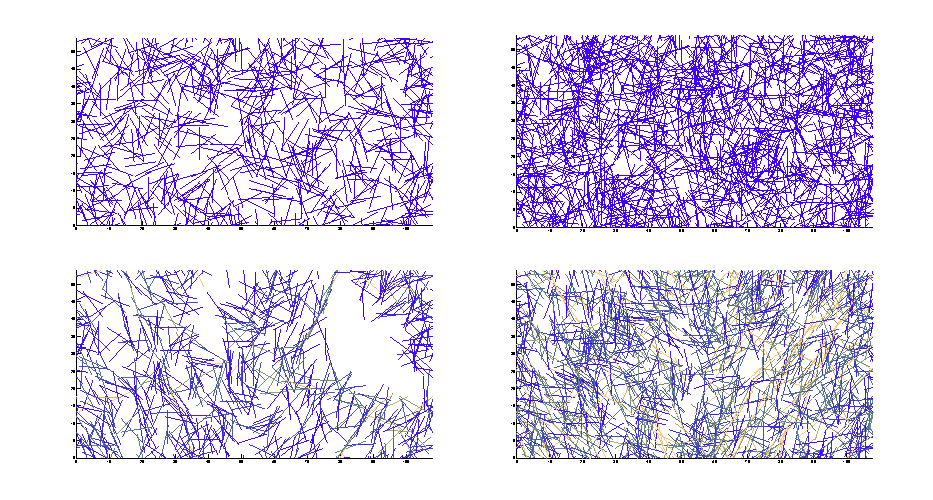
\includegraphics[width=\hsize]{network_def}
\caption{\label{fig:sim}Two Simulation setups with $L=9 \mu m, D = 54 \mu m$ before (top) and after  (bottom) 1000 seconds of applied stress. a) low density $l_c=2 \mu m$, b) moderate density $l_c=1 \mu m.  $ Scale bar $ 20 \mu m$}
\end{figure}

The nominal units for length, force, and time are $\mu m$, nN, and s, respectively.  We explored parameter space around an estimate of biologically relevant parameter values, given in Table \ref{table:para}. 

\begin{table}[h]
\centering
\caption{Simulation Parameter Values}
\label{table:para}
\begin{tabular}{|c|c|c|c|c|}
\hline
{\bf parameter}             & {\bf symbol} & {\bf physiological estimate}          \\ \hline
extensional modulus         & $\mu$        & $1 nN $                                               \\
bending modulus             & $\kappa$     & $ 10^{-3} nN \cdot \mu m$                           \\
cross-link drag coefficient & $\xi$      & $unknown $              \\
medium drag coefficient     & $\zeta$        & $0.0005 \frac{nN s}{\mu m^2} $      \\
filament length             & L            & $5 \mu m$                                          \\
cross-link spacing          & $l_c$        & $0.5 \mu m$                                         \\
domain size                 & D            & $10-50 \mu m$                                 \\ \hline
\end{tabular}
\end{table}

\begin{comment}
\begin{table}[h]
\centering
\caption{Simulation Parameter Values}
\label{table:para}
\begin{tabular}{|c|c|c|c|c|}
\hline
{\bf parameter}             & {\bf symbol} & {\bf estimated physiological value} & {\bf smallest value}           & {\bf largest value}          \\ \hline
extensional modulus         & $\mu$        & $1 nN $                             & $0.01 nN $                     & $10 nN $                     \\
bending modulus             & $\kappa$     & $ 10^{-3} nN \cdot \mu m$           & -                              & -                            \\
cross-link drag coefficient & $\xi$      & $unknown $             & $1 \frac{nN s}{\mu m} $        & $10000 \frac{nN s}{\mu m} $  \\
medium drag coefficient     & $\zeta$        & $0.0005 \frac{nN s}{\mu m^2} $      & $0.0005 \frac{nN s}{\mu m^2} $ & $0.01 \frac{nN s}{\mu m^2} $ \\
filament length             & L            & $5 \mu m$                           & $ 1\mu m$                      & $10 \mu m$                   \\
cross-link spacing          & $l_c$        & $0.5 \mu m$                         & $0.1 \mu m$                    & $2 \mu m$                    \\
domain size                 & D            & $10-50 \mu m$                       & $4\cdot L$                      & $10\cdot L$                   \\ \hline
\end{tabular}
\end{table}
\end{comment}
For computational simplicity in these models, unless otherwise mentioned we assume that the bending rigidity, $\kappa$, is infinite. This allows us to model filaments as non-bending springs of rest length, $L$, and spring modulus $\mu$.  In the appendix, we show that our result is not significantly different from the result for semi-flexible polymers.































\section{Results}

\subsection{Steady-state Approximation of Effective Viscosity}
\label{sec:eff_vic}
We begin with a calculation of a strain rate estimate of the effective viscosity for a network described by our model in the limit of highly rigid filaments.  We carry this out by assuming we have applied a constant stress along a transect of the network.  With moderate stresses, we assume the network reaches a steady state affine creep. In this situation, we would find that the stress in the network exactly balances the sum of the drag-like forces from cross-link slip.  So for any transect of length D, we have a force balance equation.

\begin{equation}
\mathbf{\sigma} = \frac{1}{D}\sum_{filaments}\: \sum_{crosslinks}\xi \cdot (\mathbf{v_i(x)}-\mathbf{v_j(x)})
\end{equation}

where $\mathbf{v_i(x)}-\mathbf{v_j(x)}$ is the difference between the velocity of a filament, $i$, and the velocity of the filament, $j$, to which it is attached at the cross-link location, $\mathbf{x}$. We can convert the sum over cross-links to an integral over the length using the average density of cross-links, $1/l_c$ and invoking the assumption of (linear order) affine strain rate, $\mathbf{v_i(x)}-\mathbf{v_j(x)}=\dot \gamma x$. This results in

\begin{multline}
\mathbf{\sigma} =  \frac{1}{D}\sum_{filaments}\:  \int_0^L \xi \cdot  \: (\mathbf{v_i(s)}-\mathbf{v_j(s)}) \:\frac{ds \cos \theta }{l_c} \\
 = \sum_{filaments}\:  \frac{\xi \dot \gamma L}{l_c} \cos \theta \cdot (x_l + \frac{L}{2} \cos \theta)
\end{multline}

Here we have introduced the variables $x_l$, and $\theta$ to describe the leftmost endpoint and the angular orientation of a given filament respectively.  Next, to perform the sum over all filaments we convert this to an integral over all orientations and endpoints that intersect our line of stress. We assume for simplicity that filament stretch and filament alignment are negligible in this low strain approximation.  Therefore, the max distance for the leftmost endpoint is the length of a filament, L, and the maximum angle as a function of endpoint is $\arccos(x_l/L)$.  The linear density of endpoints is the constant $D/l_cL$ so our integrals can be rewritten as this density over $x_l$ and $\theta$ between our maximum and minimum allowed bounds.

\begin{equation}
\mathbf{\sigma} =  \frac{1}{D} \int_0^L dx_l \int_{-\arccos (\frac{x_l}{L})}^{\arccos (\frac{x_l}{L})}\frac{d\theta}{\pi} \frac{\xi \dot \gamma L}{l_c} \cdot \frac{D}{Ll_c}\cdot (x_l \cos \theta + \frac{L}{2} cos^2\theta)
\end{equation}

Carrying out the integrals and correcting for dangling filament ends leaves us with a relation between stress and strain rate.

\begin{equation}
\mathbf{\sigma} = \frac{(L-2l_c)^2 \xi}{4\pi l_c^2} \dot \gamma 
\end{equation}

We recognize the constant of proportionality between stress and strain rate as a viscosity (in 2 dimensions).  Therefore, our approximation for the effective viscosity, $\eta_{eff}$, at steady state creep in this low strain limit is

\begin{equation}
\label{lin_eqn}
\eta_{eff} = \frac{(L-2l_c)^2 \xi}{4\pi l_c^2} .
\end{equation}

As illustrated in Figure \ref{fig:effvic}, under moderate strains ($\gamma<0.2$), our  simulations show that in the high density limit, our theoretical approximation from Eqn \ref{lin_eqn} is highly accurate at explaining the network behavior.  Aside from a geometrical factor, our approximation is valid for both shear and extensional stresses applied to the network.

As the density of the network approaches the breakdown limit, the effective viscosity diverges from our expected value.  At the low connectivities, our expected viscosity goes to 0, but the medium viscosity begins to take over as we cross the percolation threshold at $L/l_c \sim 6$.  
\begin{figure}[h!]
\centering
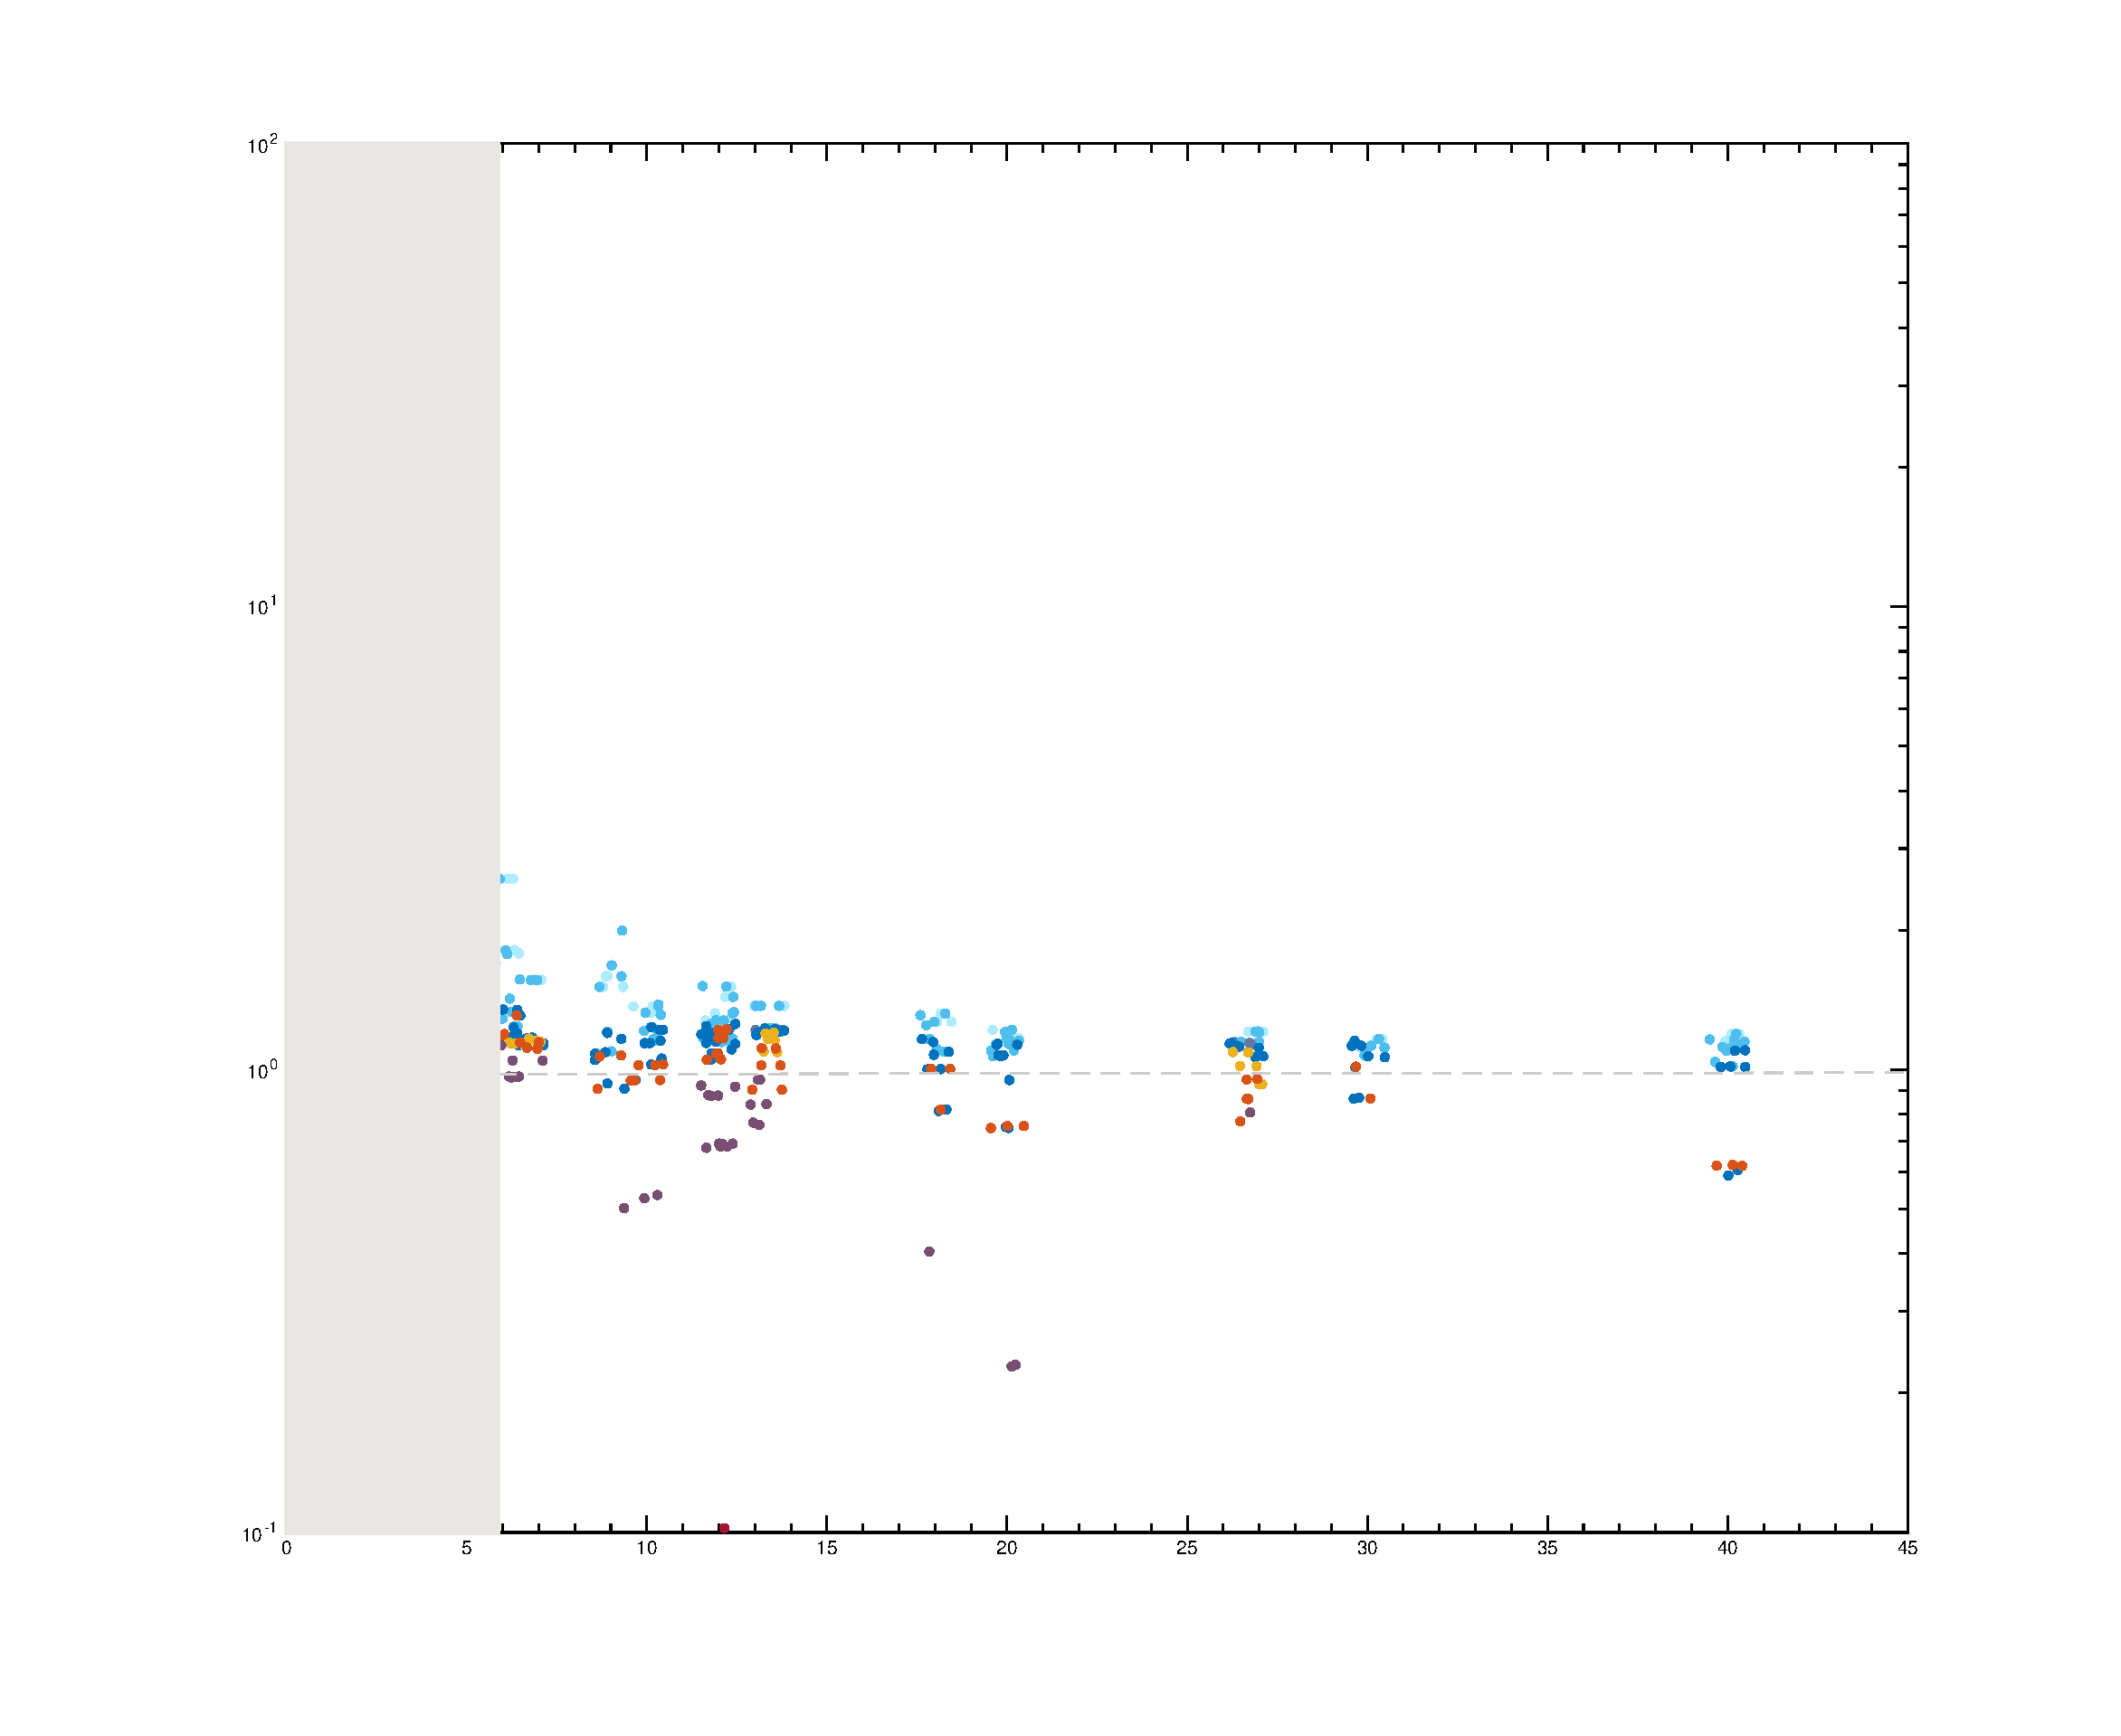
\includegraphics[width=\hsize]{eff_vic_master}
\caption{\label{fig:effvic}Ratio of effective viscosity measured by shear simulation to predicted effective viscosity as a function of connectivity, $L/l_c$. Inset: Same measurement for extensional simulations }
\end{figure}

In addition to changing the architecture and effective drag coefficient, we also validated the generality of our approximation by varying simulation size, medium viscosity, filament stiffness, and applied stress.  We were able to find a slight trend that depended on filament stiffness as indicated in the difference between blue and red data points in Figure \ref{fig:effvic}.  The deviation from our approximation and variability in results manifested itself more strongly when filaments were highly compliant.  To investigate this effect further, we next performed a more detailed analysis of the creep response while varying filament compliances.



\subsection{Effects of Filament Compliance}
\label{sec:compliant}


The effect of filament compliance on cross-linked networks under strain is a subject of active research at the moment [Sayantan].  Therefore, we wished to use our computational approach to extend our understanding of filament networks in the regime of non-negligible filament compliance.  

In irreversibly cross-linked polymer networks, filament compliance is known to give rise to elastic deformation of the network as described in\cite{theo_hlm,theo_hlm2}.    

During the initial affine deformation immediately after the application of an external stress, we see a rapid stretch of filaments, $\langle \delta L/L\rangle_0$, in response to the affine purely mechanical strain, $\gamma_{xy}$, which closely follows $\langle \delta L/L\rangle_0 = \gamma_{xy}sin(\theta)cos(\theta)$. As shown in Figure \ref{fig:glass_relax}, during the first phase in our simulations, the total network strain (solid) is described almost entirely by the strain of the filaments (dotted).  

However, in the presence of cross-link slip, the filaments are not permanently constrained to remain at $\langle \delta L/L\rangle_0$.  Interestingly, although the mean filament strain stays approximately constant, the distribution of individual filament strains broadens around the affine approximation as shown in the inset of Figure \ref{fig:glass_relax}.  

During the period where crosslink slip allows changes in the filament length distribution, we also find a long-lived intermediate relaxation phase that deviates from both the initial purely elastic relaxation and the later purely viscous behavior of section \ref{sec:eff_vic}.  In Panel B of Figure \ref{fig:glass_relax}, we show that the standard deviation of the filament stretch distribution continues to increase throughout the period that the strain rate is non constant.   

Approximating this broadening as a normally distributed variation in filament stretched length throughout the network ($\mathcal{N}$) with a time varying standard deviation, $\sigma(t)$, we have $\delta L/L = \langle \delta L/L\rangle_0 + \sigma(t)\cdot\mathcal{N}$. 
 This has an effect on the total mechanical energy stored in the network ${\cal H} \sim  \langle\delta L/L\rangle^2 = \langle\delta L/L\rangle_0^2 +\sigma(t)^2 $.   Therefore, the network will deform further while some strain energy is being stored in the further stretching filaments.  



\begin{figure}[h!]
\centering
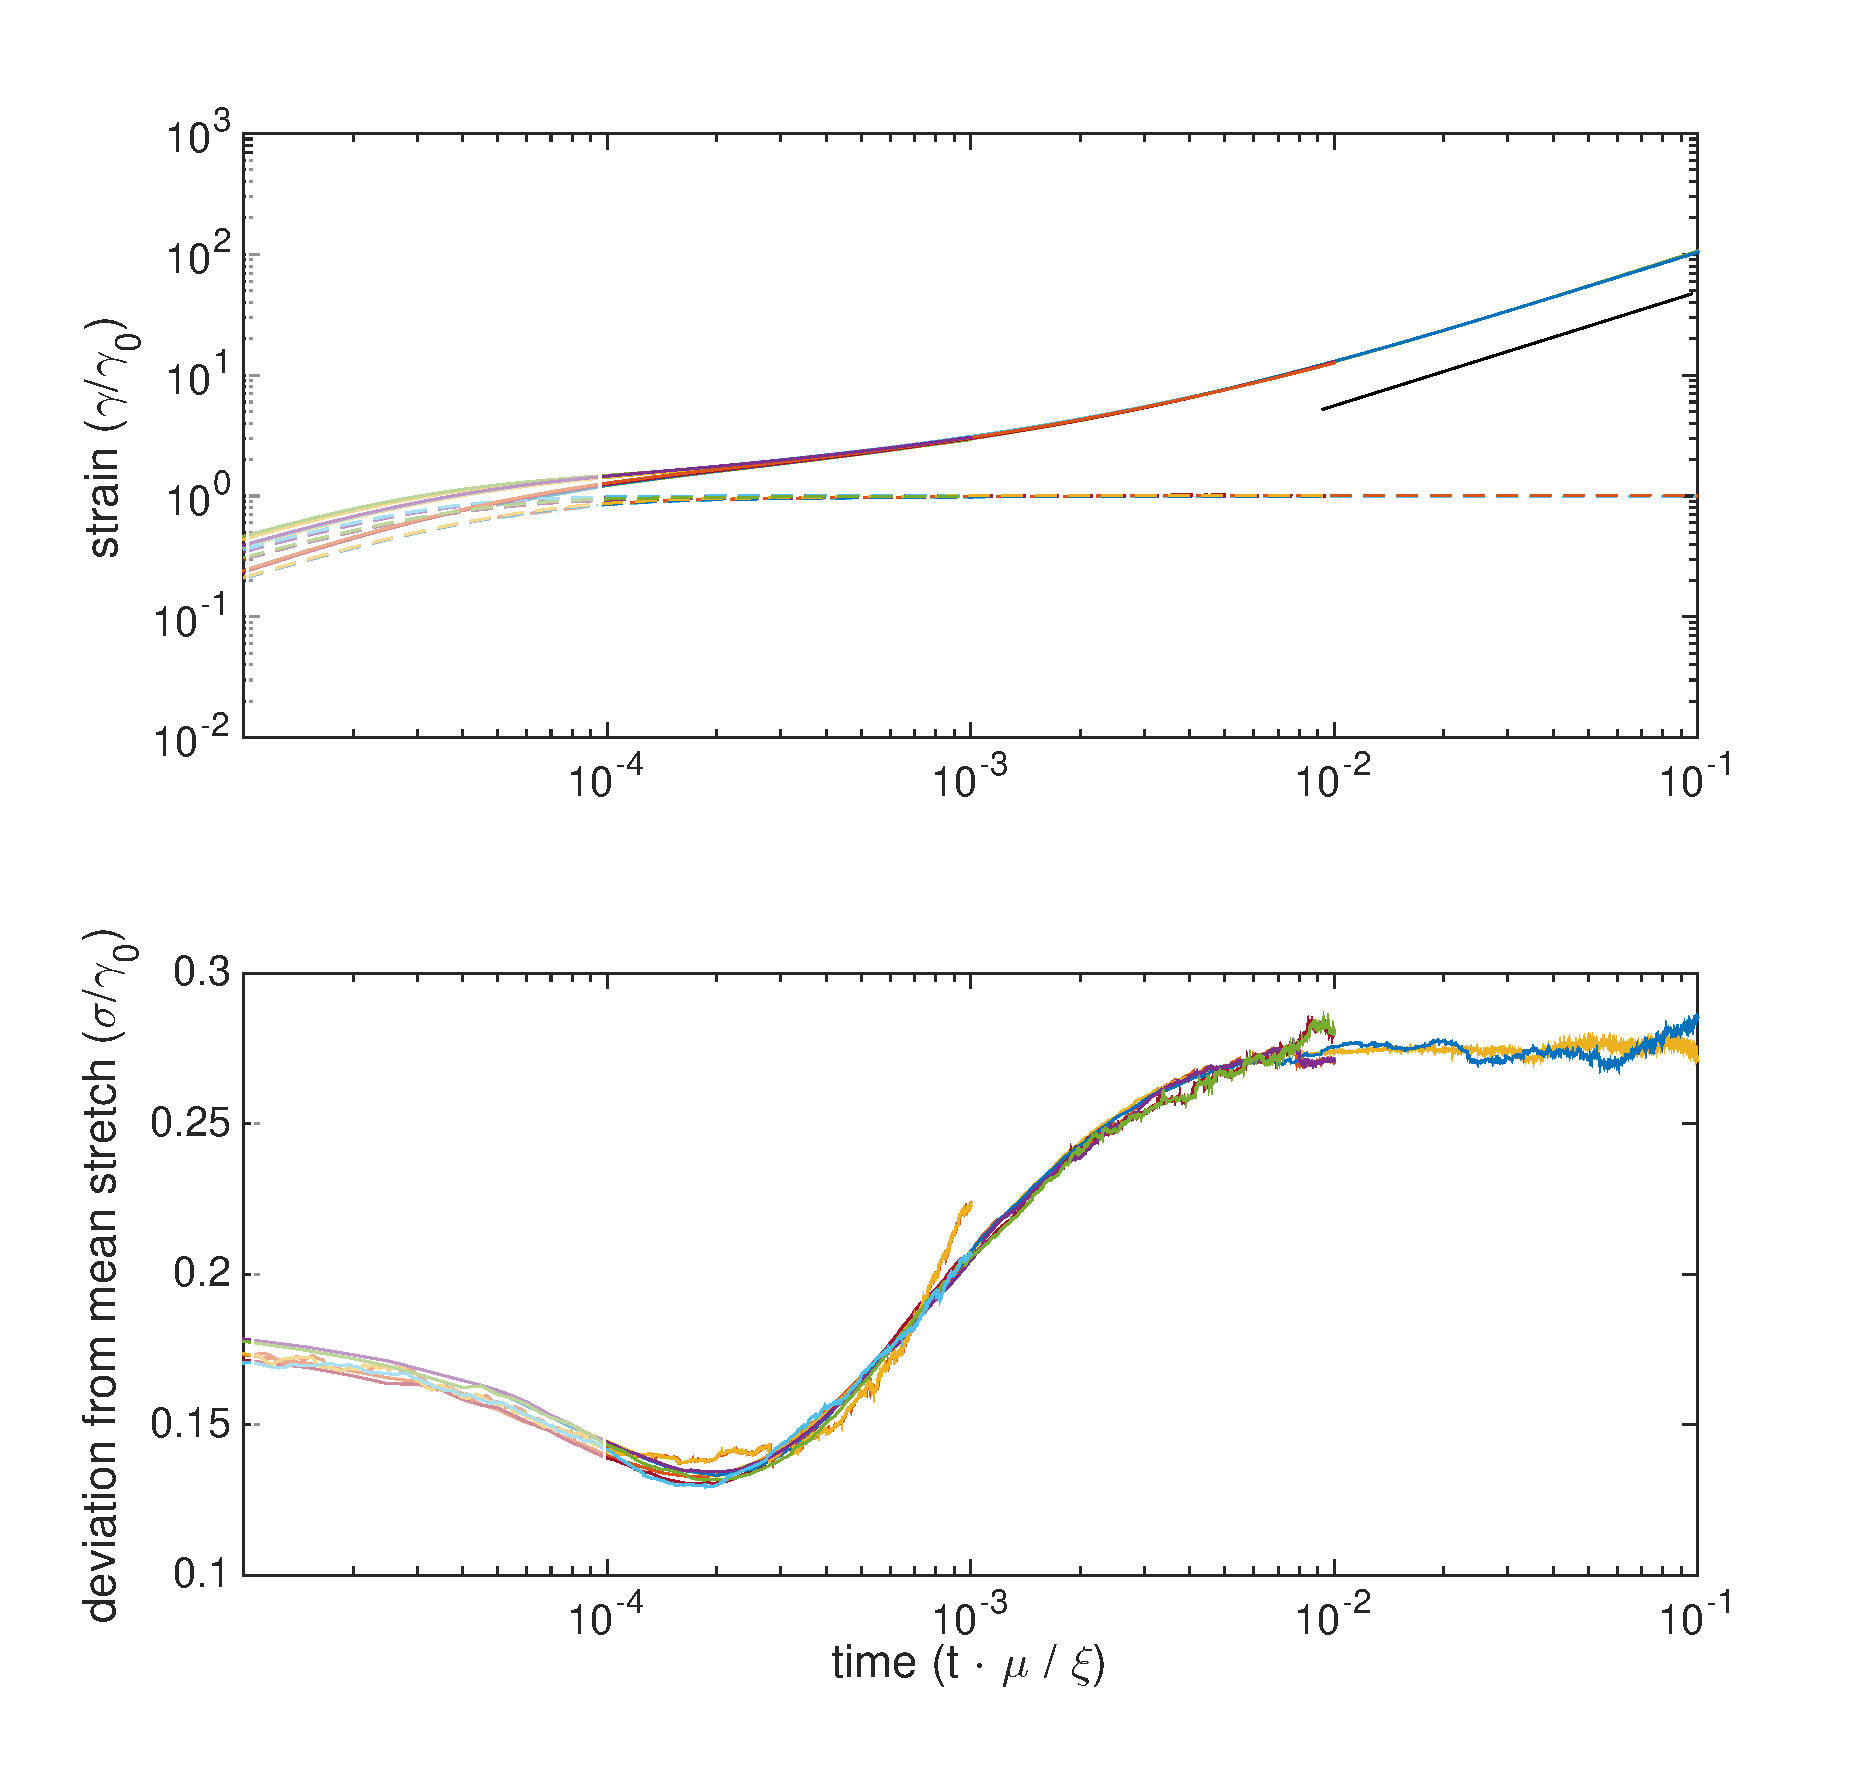
\includegraphics[width=\hsize]{glass_relax_illustrate}
\caption{\label{fig:glass_relax} Network and filament strain for different filament drag coefficient parameters.  (top) Plot of total strain normalized by the final mean filament strain, $\delta L/L$.  Dashed lines show the amount of strain from affine mechanical stretching.   (bottom) Standard deviation of filament extension for the networks in A. Note that the creep compliance in A becomes constant (slope 1) only after the spread in filament extension in B stops increasing.  Colors indicate unique experimental conditions. }
\end{figure}



Eventually the contribution from slow filament stretching will become negligible compared to that from pure cross-link slip on rigid rods.  This occurs on a timescale similar to that of cross-link slip and causes the effective viscosity to decay back toward the rigid limit.  This gives rise to a less-than-linear creep response during times after the initial elastic relaxation but before full filament relaxation from cross-link slip.   As shown in Figure \ref{fig:strain_coll}, the transition begins to take place as network strain reaches 10 to 100 times the strain from pure mechanical stretching, $\gamma_0 = \delta L / L$, and this property is independent of the magnitude of the rate of strain.  

\begin{figure}[h!]
\centering
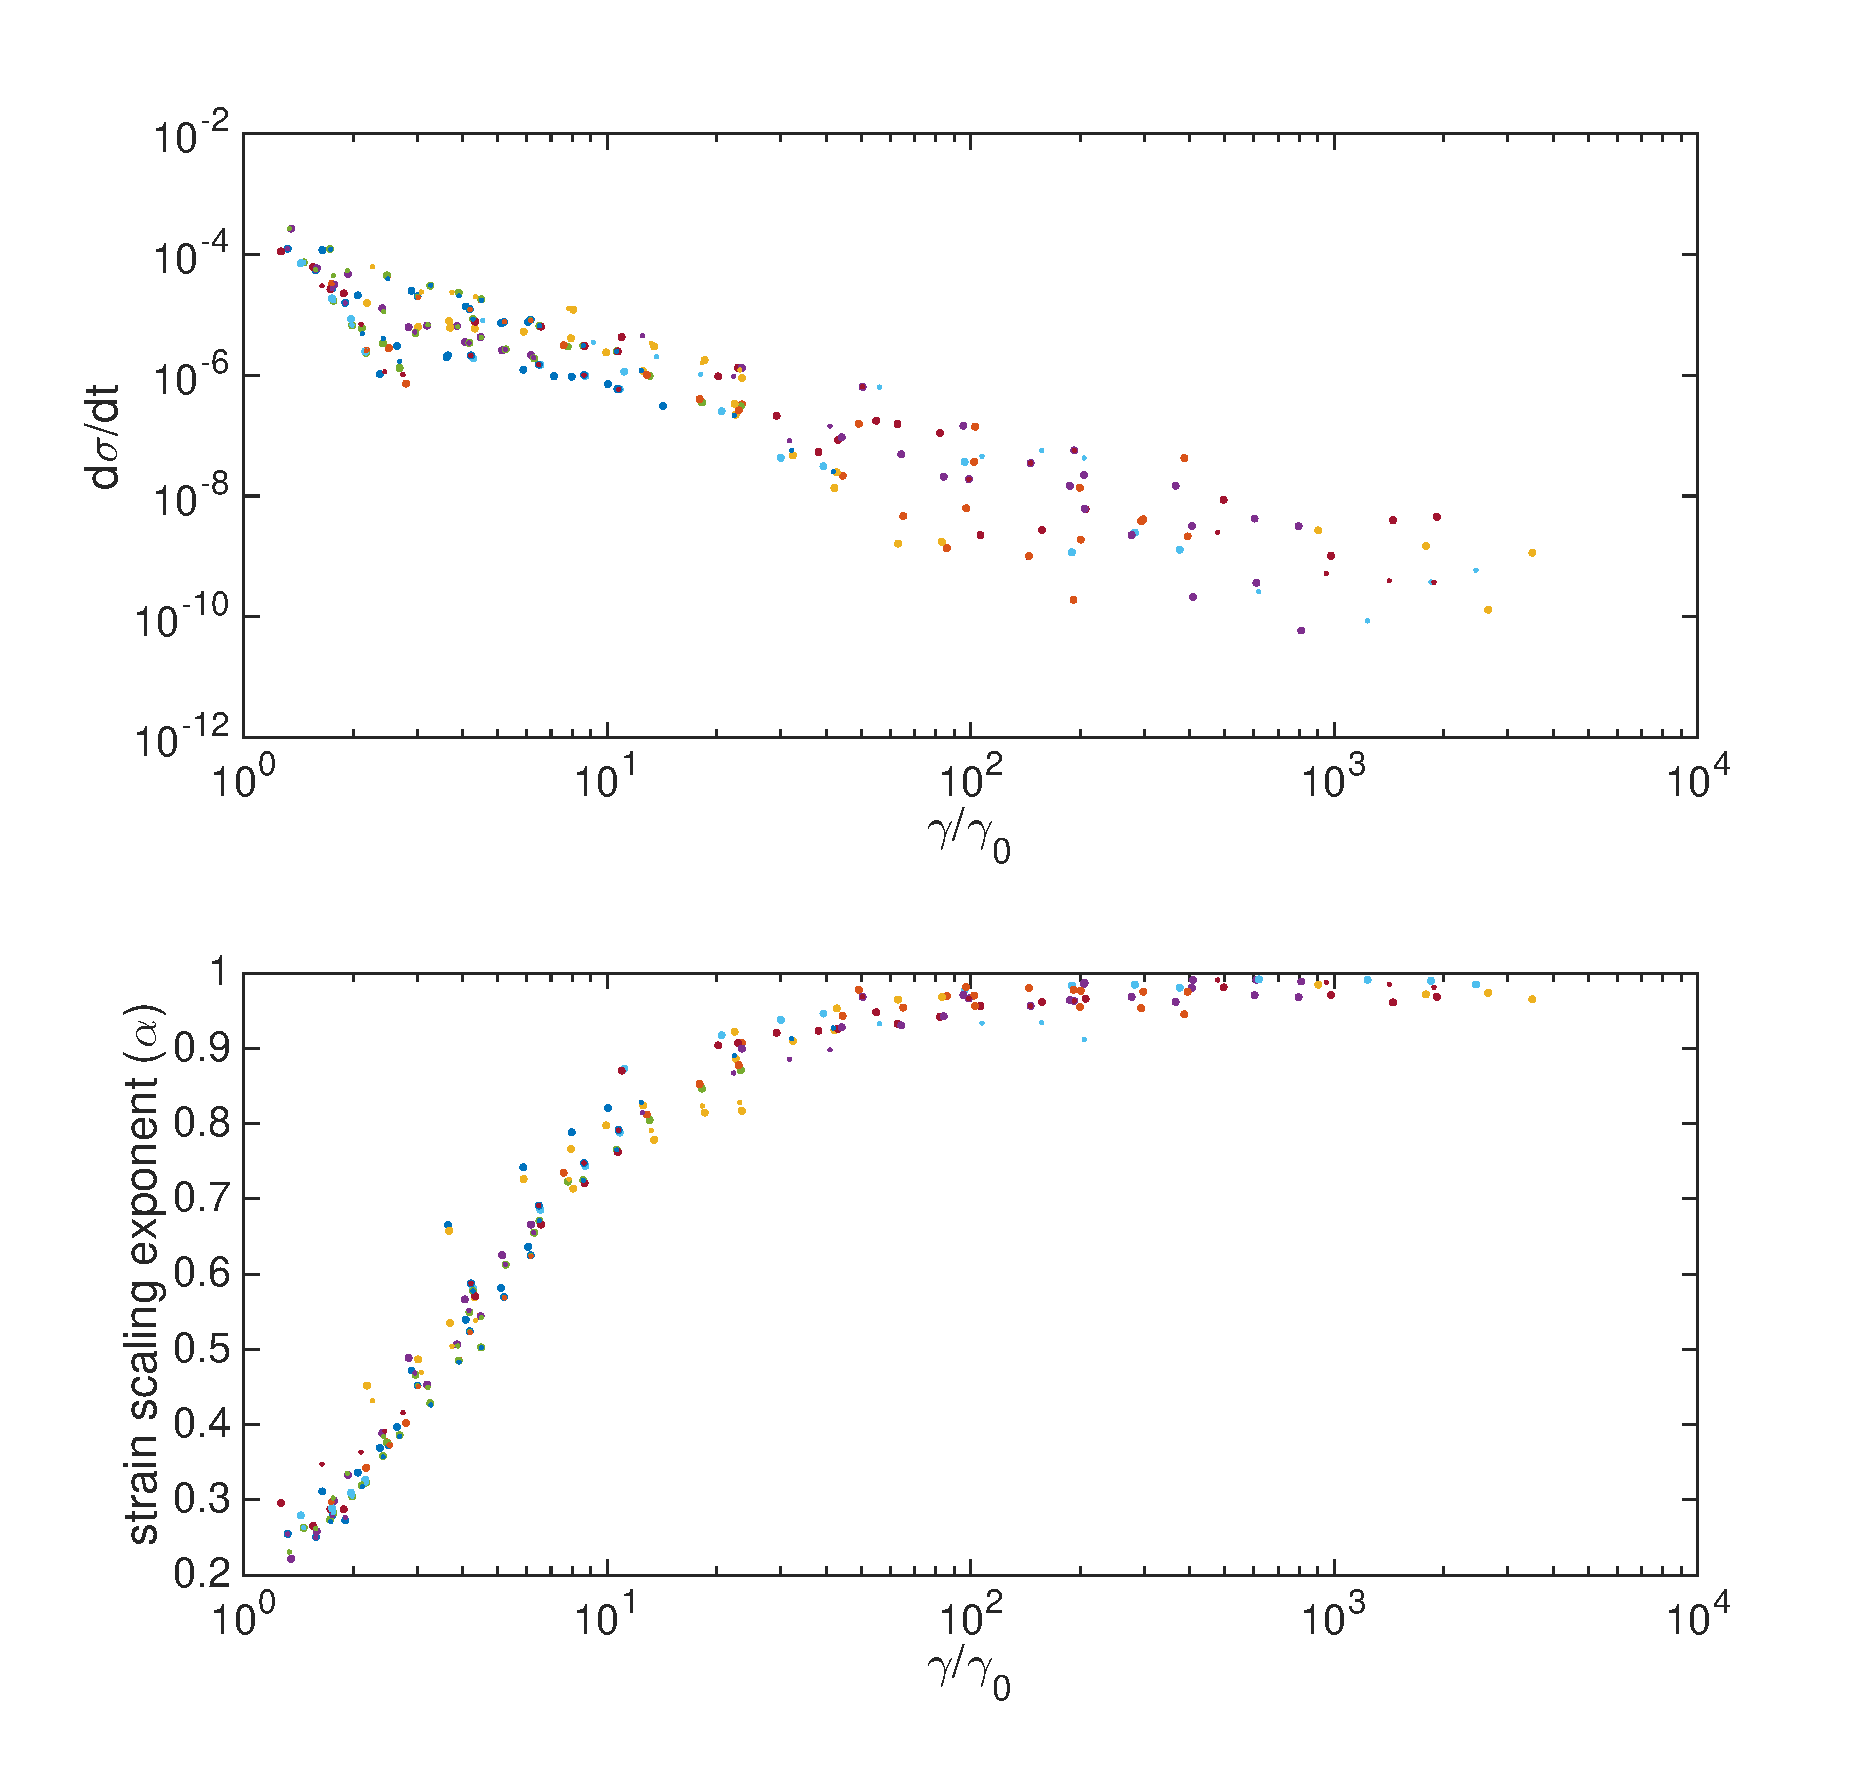
\includegraphics[width=\hsize]{collapse}
\caption{\label{fig:strain_coll} Sublinear network strain ends as change in filament strain decays. (top) Change in standard deviation of filament strain, $\sigma$, as a function of strain relative to pure mechanical strain. (bottom)   Dependence of strain rate exponent as a function of strain relative to pure mechanical strain, $\gamma_0$.  Colors indicate unique experimental conditions. }
\end{figure}




















\subsection{Alignment at High Strain and Network Tearing}

Once the network is able to accumulate a large strain, the assumption of nearly uniform distributions of filament orientations begins to break down.

At this point the filament orientations become unevenly distributed $\langle \delta L / L \rangle \neq \gamma_{xy}sin(\theta)cos(\theta)$, with a larger number of filaments aligning in the direction of extension rather than compression.  Filament alignment, conceptually, causes the formation of subdomains that no longer span the space of the network. To the authors' knowledge an exact derivation of the dependence of network connectedness on filament alignment has not been carried out, but Monte Carlo simulations have been used to show that alignment does indeed lead to lower connectedness\cite{model_percolationanisotropy}.

\begin{figure}[h!]
\centering
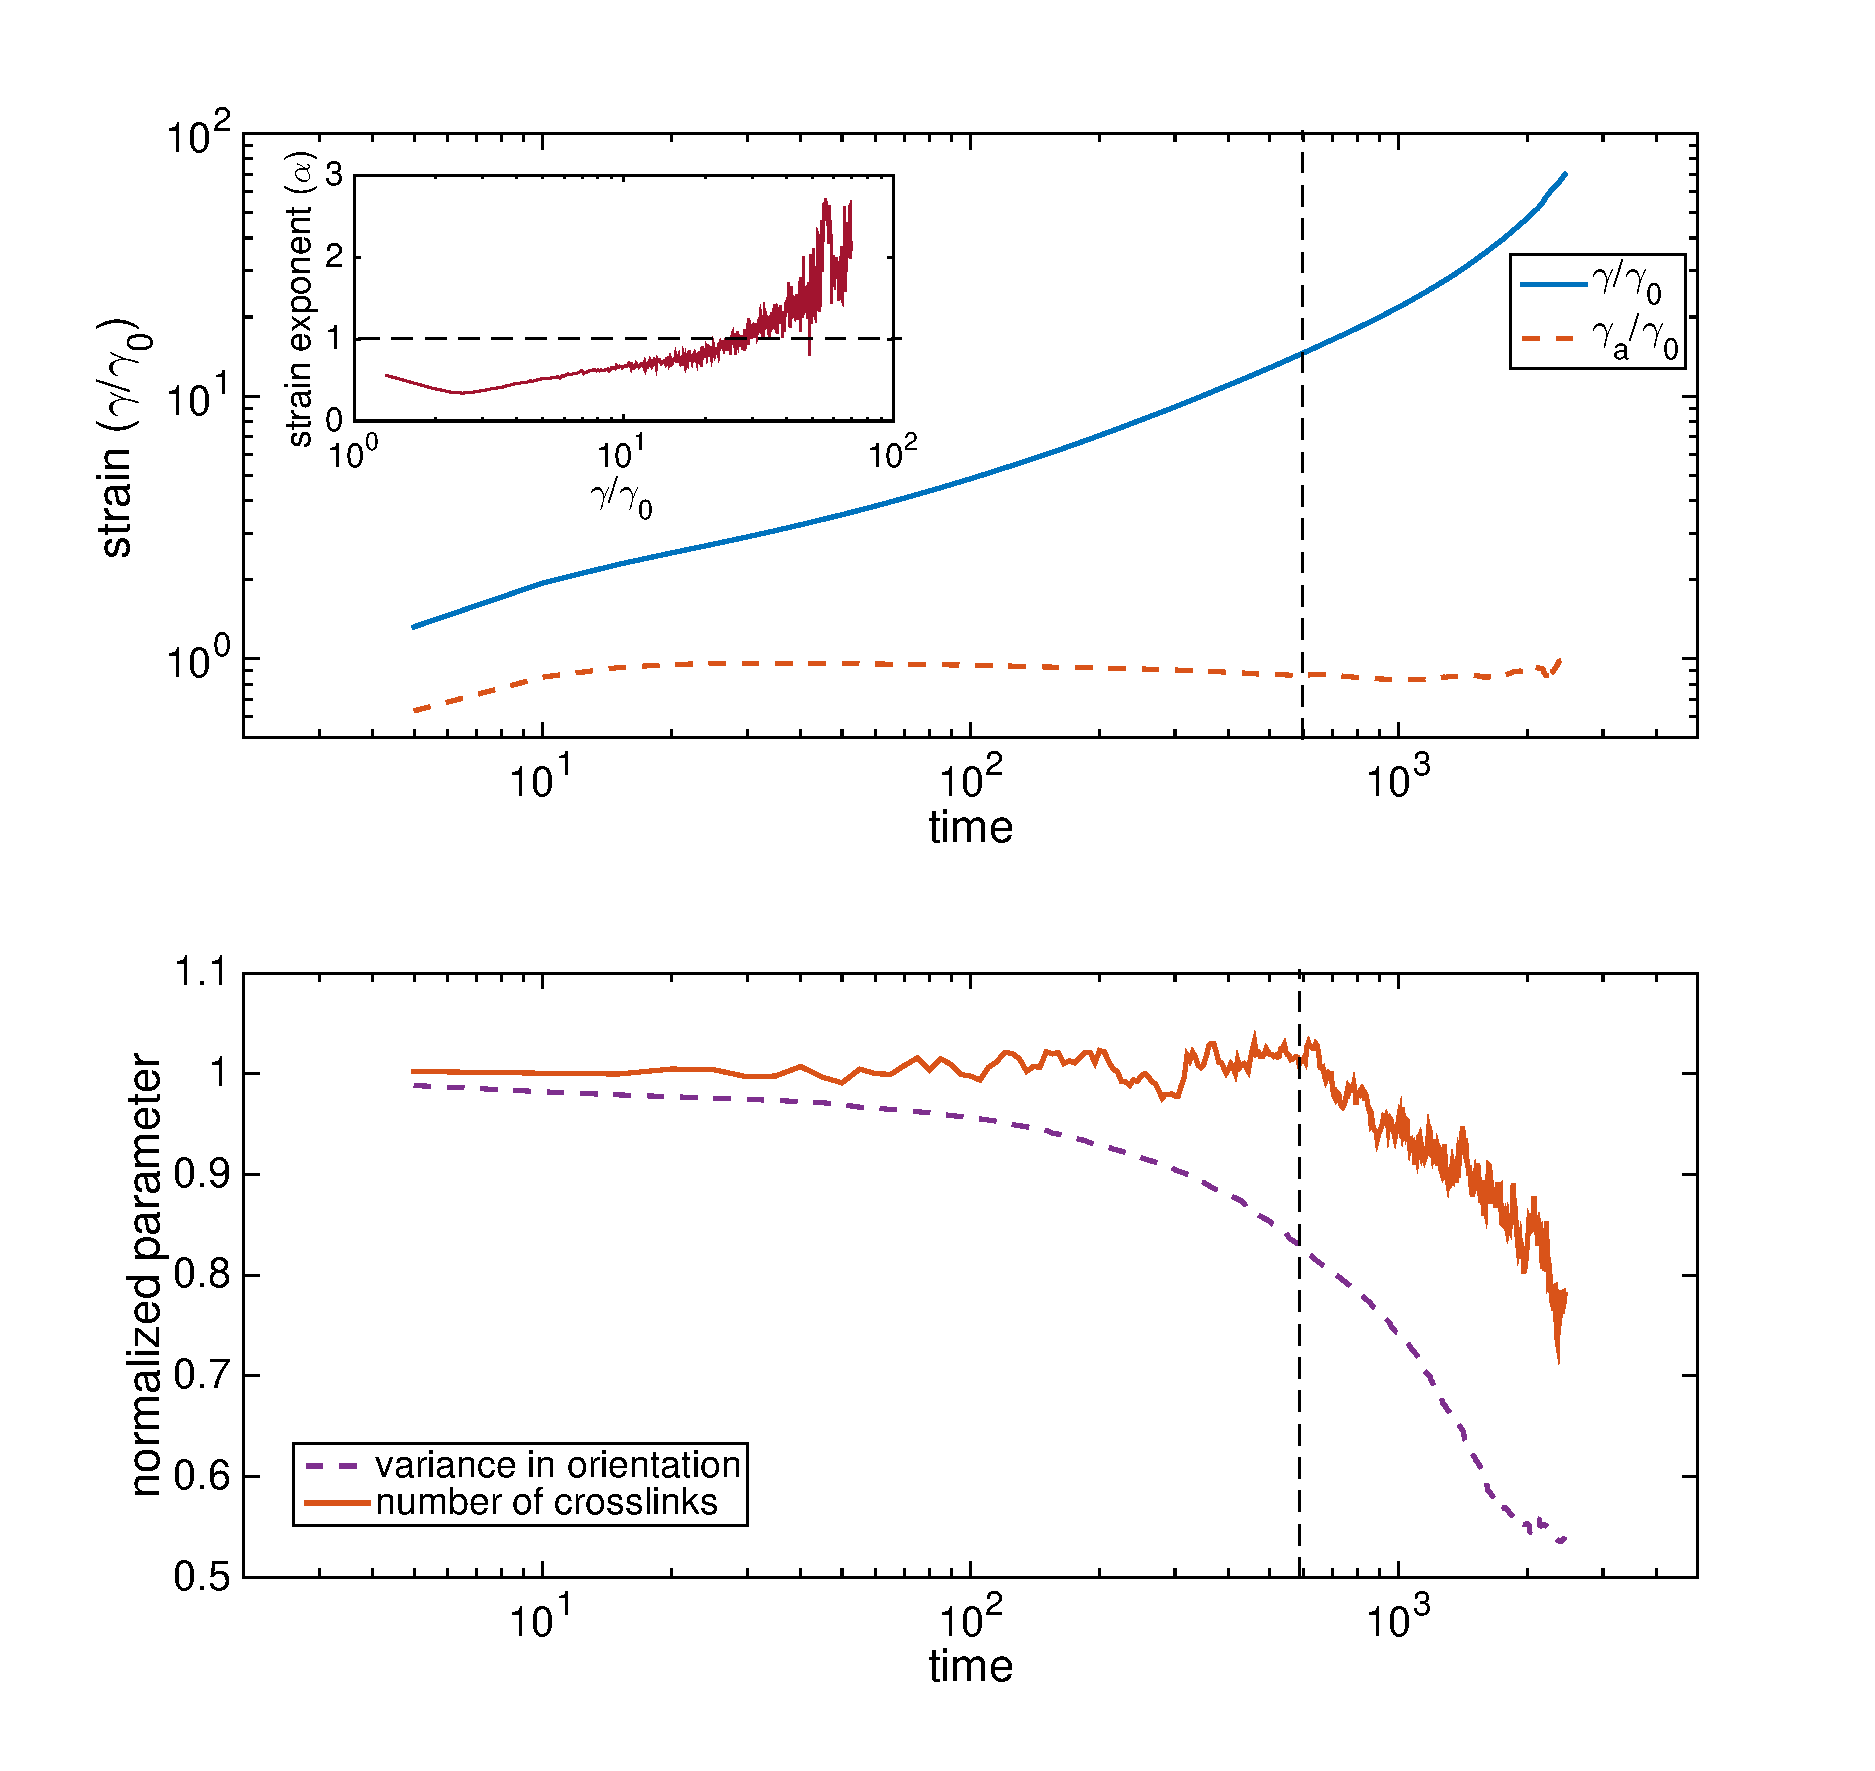
\includegraphics[width=\hsize]{tearer}
\caption{\label{fig:tearer} Creep response of a network transitioning to phase D. (top)  Strain curves for a network undergoing large scale deformation.  Inset shows strain exponent as a function of strain (exponent passes 1).  (bottom)  Traces for the variance in filament orientation and number of cross links.  Vertical dashed line shows the point where the strain exponent becomes greater than one.}
\end{figure}

We find that over time, the orientational distribution of the filaments begins to peak around 45 degrees as the large strain induces alignment.  In Figure \ref{fig:tearer}, we see that as the angular standard deviation falls, this reorientation eventually leads to fewer bonds bridging the network perpendicular to the line of strain.  As this connectivity begins to noticeably decrease, the observed effective viscosity decreases as well, giving rise to greater than linear creep.  From the inset of Figure \ref{fig:tearer} we can also see that the onset of phase D occurred before the network had completely reached phase C, leading to a rapid transition between sub-linear and super-linear creep.  Finally, it should be noted that the end of this simulation resulted in the network tearing apart.  



\subsection{Phase Diagram of Dominant Behavior}
In Figure \ref{fig:shear_modes}, we illustrate the four stereotyped phases of the general mechanical behavior that we observed in our networks.  A deforming network typically undergoes a rapid filament stretching, a slower relaxation of elastic constraints, a phase of purely viscous cross-link slippage, and an eventual alignment and breakdown of network connectivity.

\begin{figure}[h!]
\centering
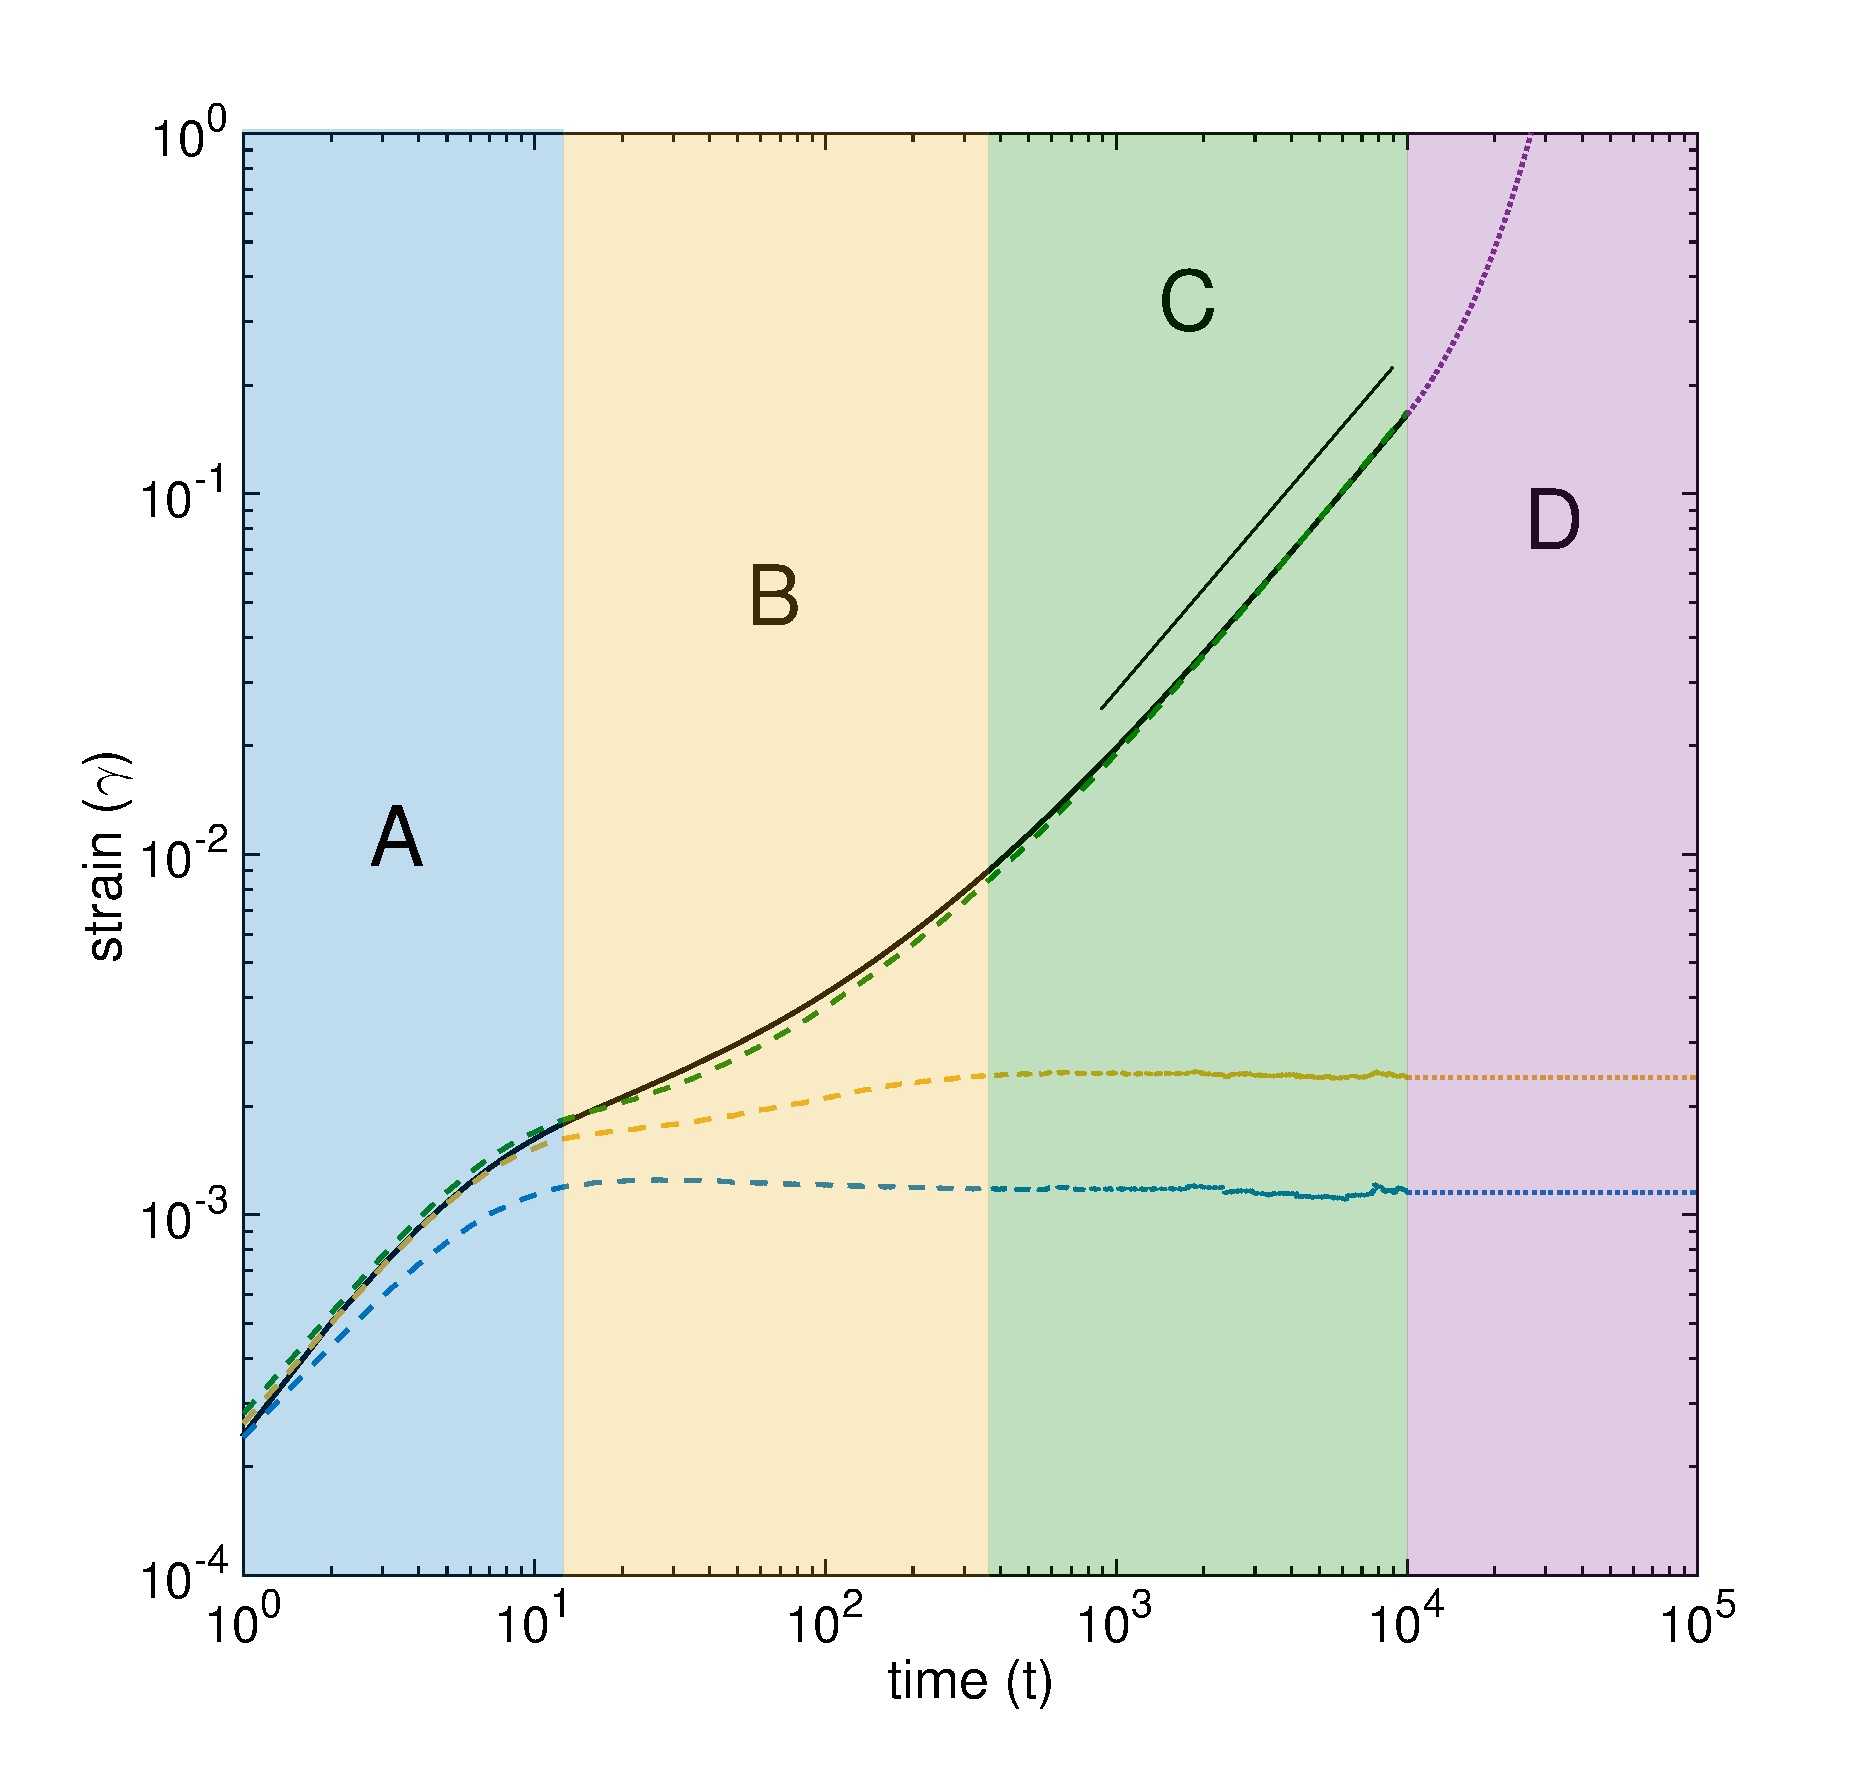
\includegraphics[width=\hsize]{shear_modes_b}
\caption{ \label{fig:shear_modes} Schematic of the general creep response of compliant filament networks illustrating the 4 phases of deformation: A) rapid mechanical response, B) combination of slow filament stretching and cross-link slip, C) cross-link slip dominated (line indicates slope of one), D) network tearing from filament alignment. Note that the portion of the curve in section D is only a hypothetical continuation of the actual data.  }
\end{figure}


Finally, to explore the transitions between the various phases, we measured the creep response for a computationally tractable network ($L/l_c = 25$), as we varied the filament extensional modulus, $\mu$, and the cross-link friction coefficient, $\xi$.  In Figure \ref{fig:phase_diag}, we classified parameter sets based on their strain exponent.  We can see the trends for the transitions between phases A, B, and C.  The line for the transition to D is still speculative at this time.  

\begin{figure}[h!]
\centering
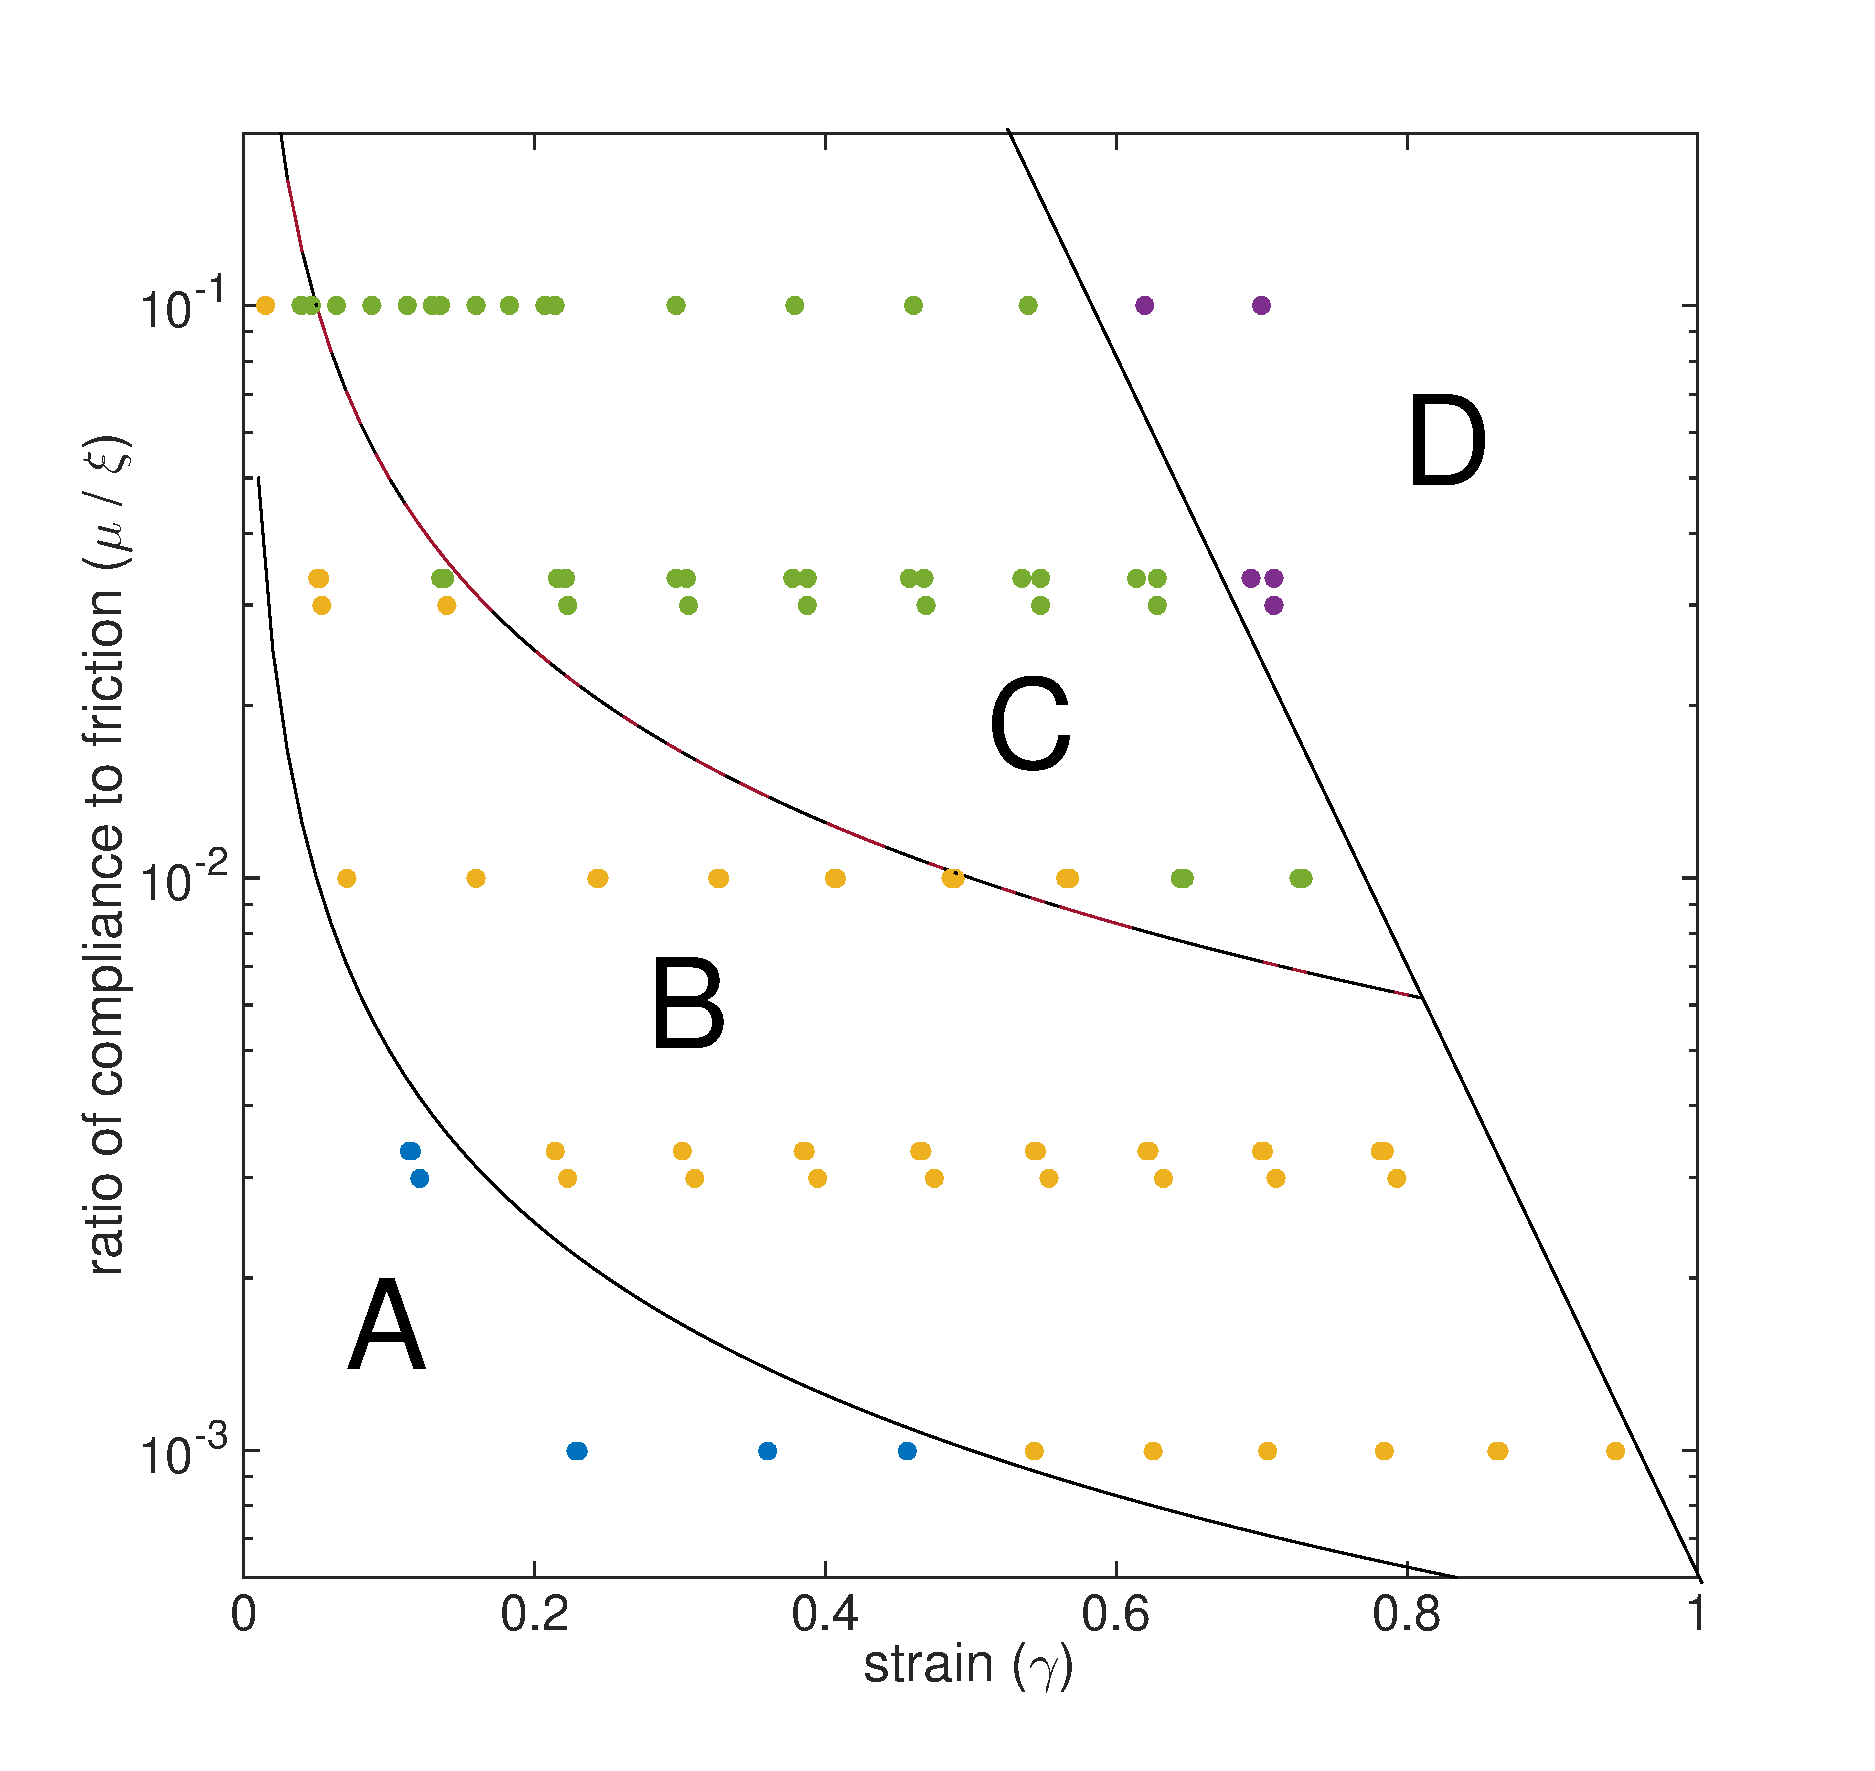
\includegraphics[width=\hsize]{phase_diag}
\caption{\label{fig:phase_diag} phase diagram of creep response for different filament extension, $\mu$ and cross-link friction, $\xi$.  Yellow, green, and purple dots correspond to creep measurements $\gamma \sim t^\alpha$ with $\alpha<0.92$, $0.92<\alpha<0.98$, or $\alpha>0.98$ respectively.  Blue dots represent creep measurements where $\gamma_{total} < 2\gamma_{mechanical}$}
\end{figure}

\begin{comment}
\subsection{Frequency dependent modulus}
This section will include a figure on the frequency dependent modulus once I get those.

\begin{figure}[h!]
\centering
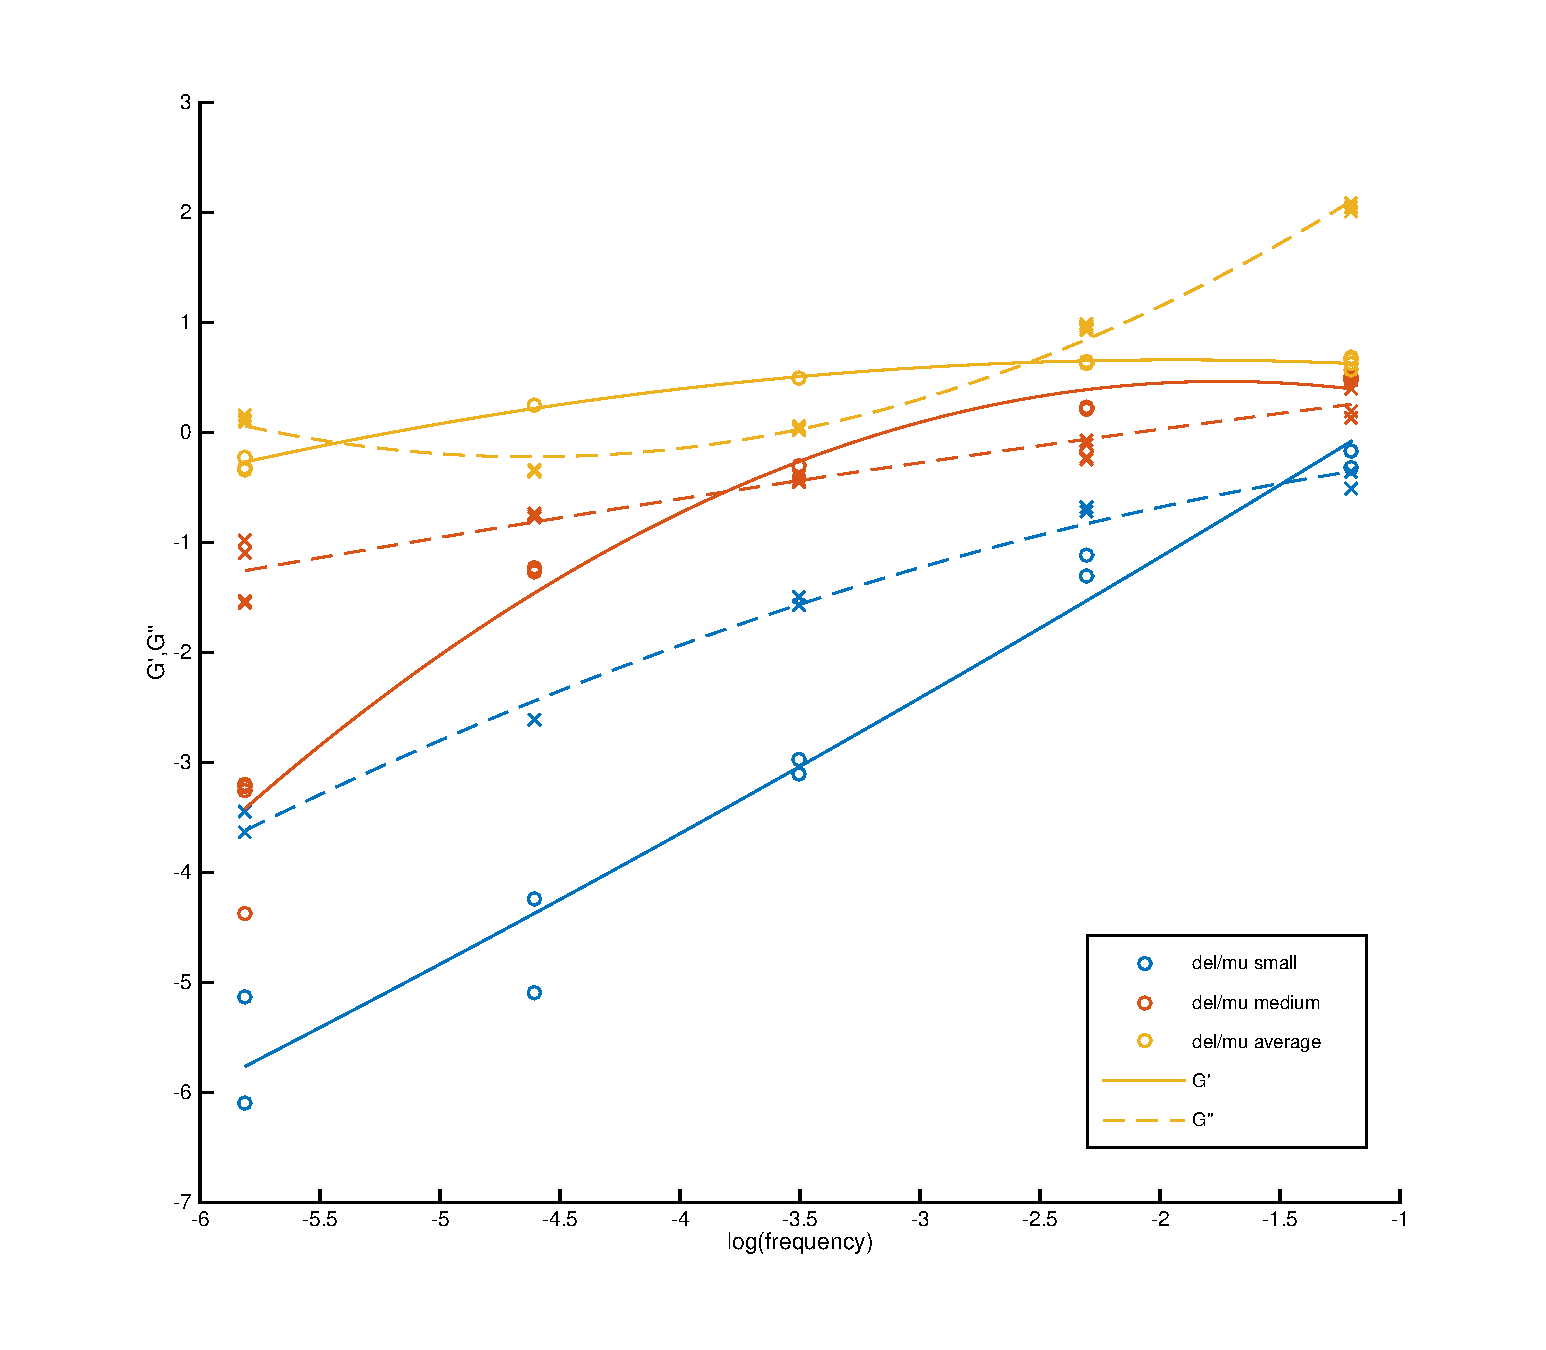
\includegraphics[width=\hsize]{frequency_dep}
\caption{\label{fig:freq} Frequency dependent moduli for networks.}
\end{figure}



\subsection{Strain Memory}
Finally, we found an interesting behavior when we introduced non-linear extensional stiffness into our filaments.  When the network is allowed to relax to it's unstrained state, there is generally a time comparable to the period of strain storage over which the energy in the network is relaxed away.  

We observed deviations from this behavior by applying stepwise stress pulses to simulated networks, and observing whether the network behaves identically upon reversal of the applied stress direction.  If the network has no strain memory then each reversal will result in an identically shaped creep curve.  However, when we include nonlinear filament extension in our model, we find that the mechanical strain can be stored for longer periods of time than it took to entrain the network.

This behavior mimics recent experiments in filamin cross-linked networks.  Filamin provides a high level of compliance to a network ($\gamma_0>0.5$) without substantial cross-link unbinding.  This allows large scale rearrangements to take place without driving very much cross-link slip, similar to the conditions in section \ref{sec:compliant}.  However, if we force individual filaments to undergo a strongly nonlinear stiffening at strains above 5\%, we find an interesting long term "strain storage."

\begin{figure}[h!]
\centering
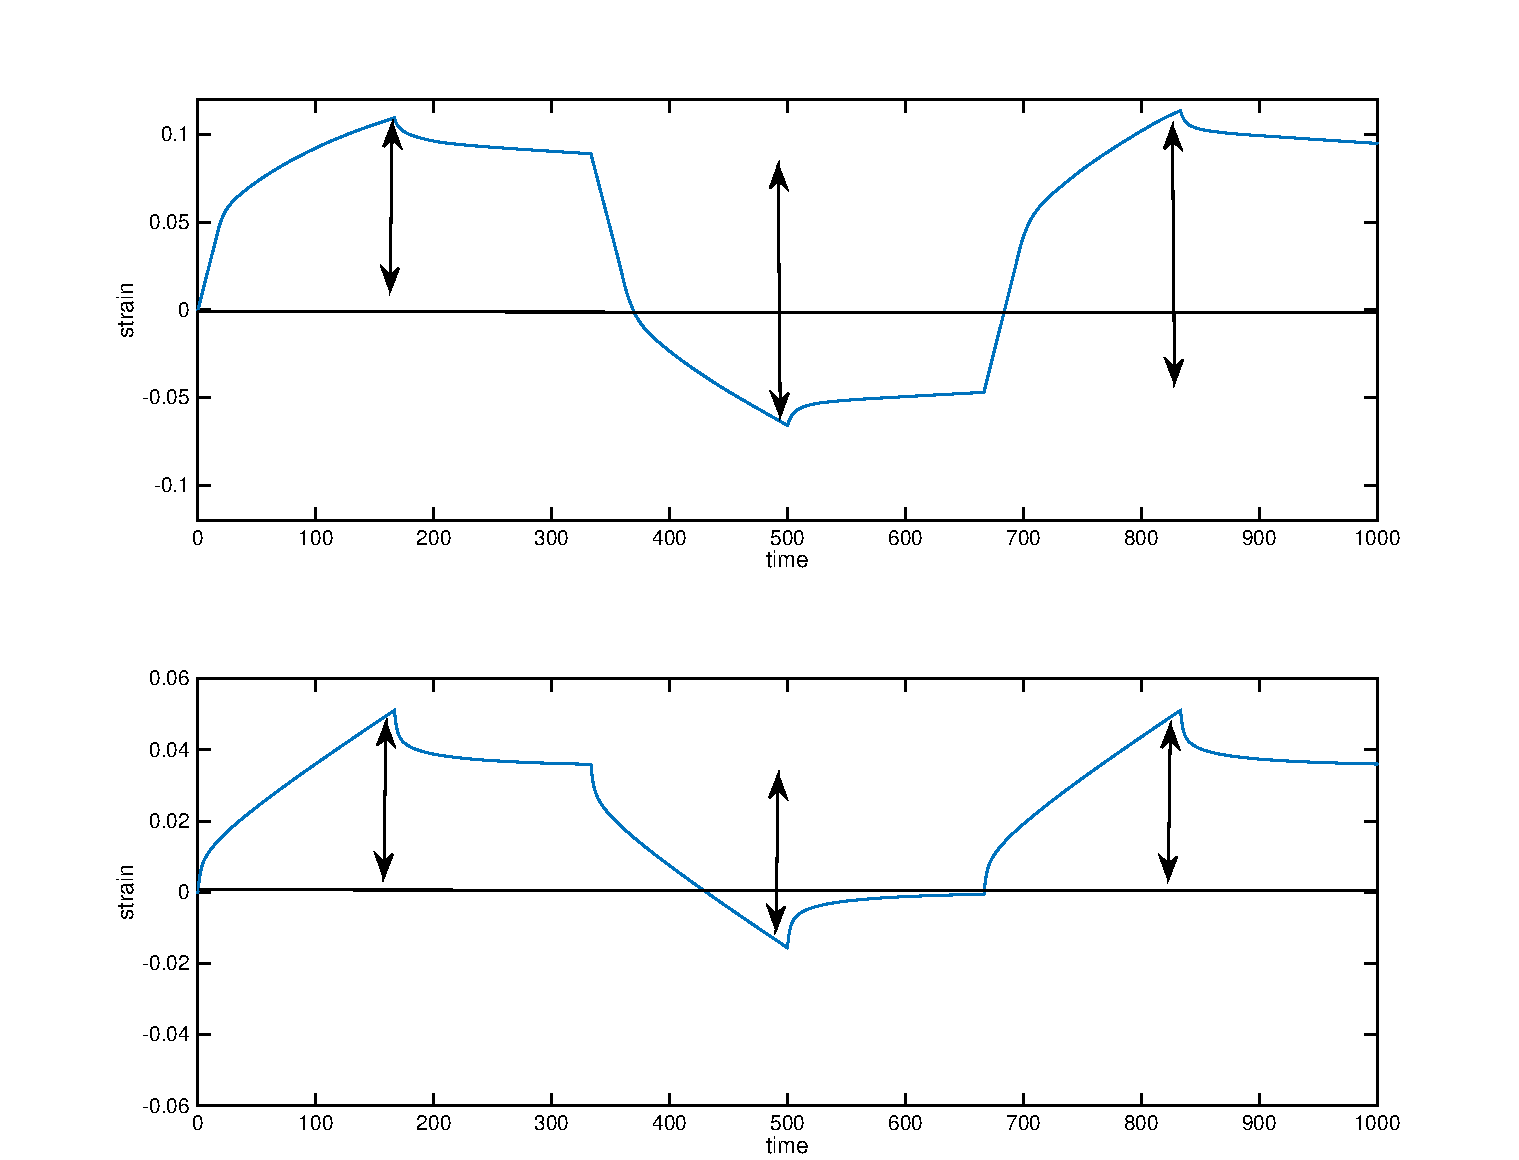
\includegraphics[width=\hsize]{strain_mem_weak}
\caption{\label{fig:strain_mem_weak} Creep curves in the presence of reversing applied stress for (a) nonlinear extension or (b) linear extension.  Note that for linear filaments the induced strain returns to approximately 0 after a complete cycle, while in the nonlinear case the cycle is not completely reversible.}
\end{figure}

Figure \ref{fig:strain_mem_weak} shows that the strain storage occurs, but I will need time for further study to build the full analytical picture of where when and why this happens in my model.
\end{comment}













\section{Summary and Conclusions}
We have proposed a simplified effective friction model for understanding 2D cross-linked networks. Our model extends previous Mikado and lattice models to include effects of cross-link relaxation. We expect that our model can confer insights into mechanisms of network stress relaxation in quasi-2D networks such as those found in \textit{in vitro} actin monolayer experiments\cite{rheo_2D1} as well as in eukaryotic actomyosin cortices\cite{cellmech_flows}.   

Our model is the first to address the plausible dependence of network effective viscosity on network structural properties.  This led to a derivation of an estimate for the long timescale creep rate of networks under constant stress.  Although this derivation neglects possible frequency dependence at short timescales, this finding offers a potential framework for addressing the dependence of network deformation rate on filament concentration and length.

Additionally, our simulations suggest that, in the presence of constant shear stress, cross-link friction will also produce a long-lived phase of sublinear creep as filaments relax from their affine stretched position. While this phase may transiently resemble more explicit 3D models such as \cite{theo_crosslinkslip1}, it is clear that our model differs by predicting that network will achieve a constant effective viscosity more rapidly.  In particular, we predict that this relaxation will occur at a rate similar to that of rate of cross-link slip derived strain and will therefore be negligible after the network has slipped by roughly ten times the magnitude of the purely affine mechanical deformation.  

In building our model we have neglected any other sources of potential mechanical relaxation in order to simplify out analysis. In the future, we hope to extend our model to include biochemically driven forms of relaxation such as filament turnover or regulated cross-link unbinding.

This model forms a basis for addressing 2D filament network deformation, and it proposes a simplified formulation of important qualitative properties. In this way we are able to address potentially general phases of network deformation and delineate what network properties may give rise to them.  This may provide an important starting point for addressing the general importance of network structure in more complex networks containing active elements. 



















\section{Acknowledgements}
I'd like to thank Shiladitya Banerjee and Sayantan Majumdar for discussions on this topic.  Hopefully I can thank other people after I've spoken with them.

















\appendix
\addappheadtotoc


\begin{comment}

\section{Network Tearing under Extensional Stress}


\subsection{Extensional Thinning and Network Tearing}

For moderate extensional stresses, the rigid filament approximation of the effective viscosity simply picks up a different geometrical factor out front.  

However, at higher stress and in the presence of different things happen.

\begin{equation}
\frac{\partial l_c}{dt}=l_c\dot \gamma =\frac{l_c \sigma}{\eta}\sim l_c^3\frac{ \sigma}{L^2 \xi}
\end{equation}

We can see that the rate of network thinning accelerates as we would expect.  When the network reaches some minimum connectivity we assume that it stops behaving as a continuum material and the network tears irreversibly.  

\begin{equation}
\tau_{break} = \frac{\eta_{eff}}{2\sigma}\cdot\left ( 1 -\frac{l_c^2}{l_{break}^2} \right )
\end{equation}

This provides us with an estimate of the timescale of catastrophic breakdown for a network with a given initial architecture and molecular drag.


\subsection{Tearing Events During Extensional Strain}

This behavior is caused primarily by the low density network undergoing tearing events that interrupt global connectedness.  

\end{comment}



\section{Deriving Molecular Drag Coefficients}
\label{app:drag}
Thus far, the idea of a molecular drag coefficient was taken as a phenomenological, measured parameter for a given experimental setup.  While this is a sufficient pragmatic justification, it's useful to try to motivate the quantitative value of this drag coefficient by connecting it to the underlying cross-link properties of binding affinity, concentration, and extensibility.

To do this we'll imagine the simplified case of two cross linkers sliding past each other in one dimension.  In this case, assume that we have an equilibrium number of bound cross-linkers, $n_B$, each of which is displaced from its equilibrium length by some distance $x$.  Each cross linker unbinds with rate $k_{off}$ and rebinds at it's relaxed position ($x=0$) with rate $k_{on}$.  At the same time, all the cross linkers are being pulled from their relaxed position at a rate, $v$, which is simply the rate at which the filaments are sliding past each other.  

We can write the differential equation for the change in the density of cross-links, $\rho$, at displacement $x$ as they are pulled upon, bind, and unbind.

\begin{equation}
\frac{\partial \rho}{\partial t} = -k_{off}\rho(x) - v\frac{\partial \rho}{\partial x} + k_{on}\delta(x)
\end{equation}

Recognizing that $\int \rho(x)=n_B$ implies $k_{on}=k_{off}n_B$, we can find the steady state solution

\begin{equation}
\rho(x) = \frac{n_b k_{off}}{v}\cdot exp\left ( -\frac{k_{off}}{v}x \right )
\end{equation}

If each cross-link has a spring constant $\mu_c$, then we can equate the force on all cross-links to the applied force that is sliding the filaments past each other.  Realistically, the spring constant and binding affinity would be functions of the cross-link stretch, but here we are taking them as approximately constant.  

\begin{equation}
\int_{0}^{\infty}\rho(x)\mu_cx dx = v \frac{\mu_c n_B}{k_{off}}= F_{app}
\end{equation}a

Therefore, the term next to v, (i.e. $\tfrac{\mu_c n_B}{k_{off}}$) would be equal to our molecular drag coefficient, $\xi$.  Assuming approximately 1 cross link per filament overlap, and using parameter estimates culled from Ferrer et al., we build the following table of estimates for $\xi$.

\begin{table}[h]
\begin{tabular}{| l | c | c |}
\hline
\textbf{cross-linker type} & $\alpha$-actinin & filamin-A  \\ \cline{1-1}
\textbf{dissociation constant ($s^{-1}$)} & 0.4 & 0.6 \\ \cline{1-1}
\textbf{spring constant ($nN / \mu m$)} & 455 & 820 \\ \cline{1-1}
\textbf{drag coefficient, $\xi$ ($\tfrac{nN \cdot s}{\mu m}$)} & 182 & 492 \\ 
\hline
\end{tabular}
\end{table}



This molecular description assumed both a constant off-rate and linear force extension of cross-links.  In the event that binding kinetics are regulated by the state of extension, we would expect (based on Rf) to find a region that exhibits a stick-slip behavior instead of the smooth.  Depending on the nature of any coupling between cross-links local stick-slip could either give rise to a global stick-slip behavior or a heterogenous mixture of stuck and sliding cross-links.  It would be interesting to explore this topic further in the future, but in the present analysis, we choose to ignore complications from these nonlinear effects.



\begin{comment}
\section{Deriving Filament and Cross-Link Composite Extensional Modulus}
\label{app:compos}
Section describing how you derive the extensional modulus.


\section{Rigid Rod Approximation with Non-Uniform Distributions of Length and Orientation}
\label{app:aargh}
Section describing how you derive the extensional modulus.



\section{Semiflexibiliy}

Brief section showing that the results are not thoroughly flummoxed by semi flexibility.

\section{Simulation details}

All changes in the force felt by an endpoint are made smooth to allow integration of the differential equation (i.e. moving between stress domains, constraint domains, and overlap coupling occurs smoothly to prevent discontinuities).  Parameter conditions that cause instabilities are excluded, and the endpoint trajectories are integrated out to at least 1000 seconds. In addition, because we wish to probe the behavior of large scale network deformations, we are neglecting the sub-dominant effects from small thermal fluctuations. 


And I think I'll probably include all the gory details of how my simulations work since I'll be wanting to have direct references to the code. 
\begin{verbatim}
double y0 = 10; // example of declaration and assignment statement
double v0 = 0;  // initial velocity
double t = 0;   // time
double dt = 0.01; // time step
double y = y0; // solved all problems
\end{verbatim}
\end{comment}
\bibliographystyle{plain}
\bibliography{slippage,active}

\end{document}


\chapter{Filament Recycling and Sustained Contractile Flows in an Actomyosin Network}
% Template for PLoS
% Version 3.1 February 2015
%
% To compile to pdf, run:
% latex plos.template
% bibtex plos.template
% latex plos.template
% latex plos.template
% dvipdf plos.template
%
% % % % % % % % % % % % % % % % % % % % % %
%
% -- IMPORTANT NOTE
%
% This template contains comments intended 
% to minimize problems and delays during our production 
% process. Please follow the template instructions
% whenever possible.
%
% % % % % % % % % % % % % % % % % % % % % % % 
%
% Once your paper is accepted for publication, 
% PLEASE REMOVE ALL TRACKED CHANGES in this file and leave only
% the final text of your manuscript.
%
% There are no restrictions on package use within the LaTeX files except that 
% no packages listed in the template may be deleted.
%
% Please do not include colors or graphics in the text.
%
% Please do not create a heading level below \subsection. For 3rd level headings, use \paragraph{}.
%
% % % % % % % % % % % % % % % % % % % % % % %
%
% -- FIGURES AND TABLES
%
% Please include tables/figure captions directly after the paragraph where they are first cited in the text.
%
% DO NOT INCLUDE GRAPHICS IN YOUR MANUSCRIPT
% - Figures should be uploaded separately from your manuscript file. 
% - Figures generated using LaTeX should be extracted and removed from the PDF before submission. 
% - Figures containing multiple panels/subfigures must be combined into one image file before submission.
% For figure citations, please use "Fig." instead of "Figure".
% See http://www.plosone.org/static/figureGuidelines for PLOS figure guidelines.
%
% Tables should be cell-based and may not contain:
% - tabs/spacing/line breaks within cells to alter layout or alignment
% - vertically-merged cells (no tabular environments within tabular environments, do not use \multirow)
% - colors, shading, or graphic objects
% See http://www.plosone.org/static/figureGuidelines#tables for table guidelines.
%
% For tables that exceed the width of the text column, use the adjustwidth environment as illustrated in the example table in text below.
%
% % % % % % % % % % % % % % % % % % % % % % % %
%
% -- EQUATIONS, MATH SYMBOLS, SUBSCRIPTS, AND SUPERSCRIPTS
%
% IMPORTANT
% Below are a few tips to help format your equations and other special characters according to our specifications. For more tips to help reduce the possibility of formatting errors during conversion, please see our LaTeX guidelines at http://www.plosone.org/static/latexGuidelines
%
% Please be sure to include all portions of an equation in the math environment.
%
% Do not include text that is not math in the math environment. For example, CO2 will be CO\textsubscript{2}.
%
% Please add line breaks to long display equations when possible in order to fit size of the column. 
%
% For inline equations, please do not include punctuation (commas, etc) within the math environment unless this is part of the equation.
%
% % % % % % % % % % % % % % % % % % % % % % % % 
%
% Please contact latex@plos.org with any questions.
%
% % % % % % % % % % % % % % % % % % % % % % % %

\documentclass[10pt,letterpaper]{article}
\usepackage[top=0.85in,left=2.75in,footskip=0.75in]{geometry}

% Use adjustwidth environment to exceed column width (see example table in text)
\usepackage{changepage}

% Use Unicode characters when possible
\usepackage[utf8]{inputenc}

% textcomp package and marvosym package for additional characters
\usepackage{textcomp,marvosym}

% fixltx2e package for \textsubscript
\usepackage{fixltx2e}

% amsmath and amssymb packages, useful for mathematical formulas and symbols
\usepackage{amsmath,amssymb}

% cite package, to clean up citations in the main text. Do not remove.
\usepackage{cite}

% Use nameref to cite supporting information files (see Supporting Information section for more info)
\usepackage{nameref,hyperref}

% line numbers
\usepackage[right]{lineno}

% ligatures disabled
\usepackage{microtype}
\DisableLigatures[f]{encoding = *, family = * }

% rotating package for sideways tables
\usepackage{rotating}

\usepackage{verbatim}   % useful for program listings

% Remove comment for double spacing
%\usepackage{setspace} 
%\doublespacing

% Text layout
\raggedright
\setlength{\parindent}{0.5cm}
\textwidth 5.25in 
\textheight 8.75in

% Bold the 'Figure #' in the caption and separate it from the title/caption with a period
% Captions will be left justified
\usepackage[aboveskip=1pt,labelfont=bf,labelsep=period,justification=raggedright,singlelinecheck=off]{caption}

% Use the PLoS provided BiBTeX style
% \bibliographystyle{plos2015}
\bibliographystyle{apalike}

% Remove brackets from numbering in List of References
\makeatletter
\renewcommand{\@biblabel}[1]{\quad#1.}
\makeatother

% Leave date blank
\date{}

% Header and Footer with logo
\usepackage{lastpage,fancyhdr,graphicx}
\usepackage{epstopdf}
\pagestyle{myheadings}
\pagestyle{fancy}
\fancyhf{}
\lhead{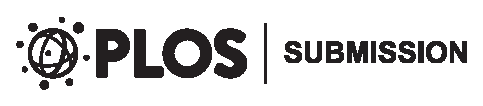
\includegraphics[width=2.0in]{PLOS-submission.eps}}
\rfoot{\thepage/\pageref{LastPage}}
\renewcommand{\footrule}{\hrule height 2pt \vspace{2mm}}
\fancyheadoffset[L]{2.25in}
\fancyfootoffset[L]{2.25in}
\lfoot{\sf PLOS}

%% Include all macros below

\newcommand{\lorem}{{\bf LOREM}}
\newcommand{\ipsum}{{\bf IPSUM}}

%% END MACROS SECTION


\begin{document}
\vspace*{0.35in}

% Title must be 250 characters or less.
% Please capitalize all terms in the title except conjunctions, prepositions, and articles.
\begin{flushleft}
{\Large
\textbf\newline{Filament Recycling and Sustained Contractile Flows in an Actomyosin Cortex}
}
\newline
% Insert author names, affiliations and corresponding author email (do not include titles, positions, or degrees).
\\
William M McFadden\textsuperscript{1},
Patrick M McCall\textsuperscript{2},
Edwin M Munro\textsuperscript{3,*}
\\
\bigskip
\bf{1} Biophysical Sciences Program, University of Chicago, Chicago, IL, USA
\\
\bf{2} Department of Physics, University of Chicago, Chicago, IL, USA
\\
\bf{3} Department of Molecular Genetics and Cell Biology, University of Chicago, Chicago, IL, USA
\\
\bigskip

% Insert additional author notes using the symbols described below. Insert symbol callouts after author names as necessary.
% 
% Remove or comment out the author notes below if they aren't used.
%
% Primary Equal Contribution Note
%\Yinyang These authors contributed equally to this work.

% Additional Equal Contribution Note
% Also use this double-dagger symbol for special authorship notes, such as senior authorship.
%\ddag These authors also contributed equally to this work.

% Current address notes
%\textcurrency a Insert current address of first author with an address update
% \textcurrency b Insert current address of second author with an address update
% \textcurrency c Insert current address of third author with an address update

% Deceased author note
%\dag Deceased

% Group/Consortium Author Note
%\textpilcrow Membership list can be found in the Acknowledgments section.

% Use the asterisk to denote corresponding authorship and provide email address in note below.
* emunro@uchicago.edu

\end{flushleft}
% Please keep the abstract below 300 words
\section*{Abstract}
Fill in abstract later.


% Please keep the Author Summary between 150 and 200 words
% Use first person. PLOS ONE authors please skip this step. 
% Author Summary not valid for PLOS ONE submissions.   
\section*{Author Summary}
In this paper, we develop and analyze a minimal model for 2D active networks based on the cortical cytoskeleton of eukaryotic embryos.  Our model introduces a series of coarse-grained approximations for simultaneous comparison of cross-link stress dissipation, myosin driven active stress generation and a form of rapid filament turnover we term {\em filament recycling}.  We generate computational simulations based on the model and demonstrate that our minimal assumptions are sufficient to drive network contraction and to set up steady state flow profiles such as those found in the cortex of developing embryos and migrating cells.  Our analysis sheds insight on potential microscopic control parameters governing broad qualitative differences in 2D active networks. 
\linenumbers

\section*{Introduction}

\paragraph{}  Cortical flow is a fundamental and ubiquitous form of cellular deformation that underlies cell polarization, cell division, cell crawling and multicellular tissue morphogenesis\cite{cellmech_flows3,cellmech_flows2}.  These flows arise within the actomyosin cortex, a thin layer of cross-linked actin filaments and myosin motors that lies just beneath the plasma membrane \cite{Salbreux2012536}. The active forces that drive cortical flows are thought to be generated by myosin motors pulling against individual actin filaments \cite{Munro2004413}. These forces must be integrated within cross-linked networks to build macroscopic contractile stress.  At the same time, cross-linked networks resist deformation and this resistance must be dissipated by network remodeling to allow macroscopic network deformation and flow.  How force production and dissipation depend on motor activity, network architecture and remodeling remains poorly understood.

Current models for cortical flow rely on coarse-grained descriptions of actomyosin networks as active fluids, whose motions are driven by gradients of active contractile stress and opposed by an effectively viscous resistance\cite{cellmech_flows}.  In these models, gradients of active stress are assumed to reflect spatial variation in motor activity and viscous resistance is assumed to reflect the internal dissipation of elastic resistance due to local remodeling of filaments and/or cross-links \cite{PhysRevLett.106.028103}.  A key virtue of these models is that their behavior is governed by a few parameters (active stress and effective viscosity).  By coupling an active fluid description to simple kinetic models for network assembly and disassembly and making active stress and effective viscosity depend on e.g network density and turnover rates, it is possible to capture phenomenological descriptions of cortical flow.  Models based on this active fluids description can successfully reproduce spatiotemporal dynamics of cortical flow observed during polarization \cite{cellmech_flows}, cell division \cite{Turlier2014114,PhysRevLett.103.058102}, cell motility \cite{Keren:2009aa,RevModPhys.85.1143} and tissue morphogenesis \cite{Heisenberg2013948}.  

However, to understand how cells exert physiological control over cortical deformation and flow, or to build and tune networks with desired properties {\em in vitro}, it is essential to connect this coarse-grained description to the microscopic origins of force generation and dissipation within cross-linked actomyosin networks.  Both active stress and effective viscosity depend sensitively on microscopic parameters including densities of filaments, motors and cross-links, force-dependent motor/filament interactions, cross-link dynamics and network turnover rates.  Thus a key challenge is to understand how tuning these microscopic parameters controls the dynamic interplay between active force generation and passive relaxation to control macroscopic dynamics of cortical flow.

\paragraph{} Studies in living cells have documented fluid-like stress relaxation on timescales of 10-100s of seconds \cite{cellmech_flows,cellmech_flows2,cellmech_flows3,rheo_fluid,rheo_fluid2,cell_rheo_exp}.  These modes of stress relaxation are thought to arise both from the transient binding/unbinding of individual cross-links and from the turnover (assembly/disassembly) of actin filaments (ref).  Studies of cross-linked and/or bundled actin networks {\em in vitro} suggest that cross-link unbinding may be sufficient to support viscous relaxation (creep) on very long timescales\cite{rheo_crosslinksmatter,rheo_crosslinkslip1,rheo_crosslinkslip2,rheo_crosslinkslip3,rheo_nonaffine}, but is unlikely to explain the rapid large scale cortical deformation and flow observed in living cells.  It has been proposed in the field that rapid actin turnover must play a significant role as well. Indeed, photokinetic and single molecule imaging studies studies reveal rapid turnover of cortical actin filaments in living cells on timescales of 10-100 seconds \cite{Robin:2014aa}. Previous theoretical models have explored  the dependence of stress relaxation on cross-link binding and unbinding analytically \cite{theo_crosslinkslip1,theo_crosslinkslip2} and others have explicitly modeled reversible cross-linking in combination with complex mechanics of filament bundles \cite{model_taeyoon,rheo_crosslinkslip2,theo_crosslinkslip3}, leading to complex viscoelastic stress relaxation.  However, until very recently \cite{Mak:2016aa} very little attention has been paid to actin turnover as mechanism of stress relaxation. 

Recent work has also begun to reveal insights into mechanisms that govern active stress generation in disordered actomyosin networks. In vitro studies have confirmed that local interactions among actin filaments and myosin motors are sufficient to drive macroscopic contraction of disordered networks \cite{rheo_2D1}.  Theoretical studies suggest that asymmetrical compliance of actin filaments (stiffer under extension than compression) and spatial differences (dispersion) in motor activity are sufficient conditions for contraction in one \cite{1367-2630-14-3-033037} and two \cite{PhysRevX.4.041002} dimensional networks, although other routes to contractility may also exist \cite{PhysRevX.4.041002}.  Further work has explored how modulation of network architecture, cross-link dynamics and motor density, activity and assembly state can shape rates and patterns of network deformation \cite{10.1371/journal.pone.0039869,Alvarado:2013aa,C0SM00494D} or network rheology \cite{0295-5075-85-1-18007,rheo_active}.  

Significantly, {\em in vitro} models for disordered actomyosin networks have used stable actin filaments, and these networks support only transient contraction, either because of network collapse\cite{Alvarado:2013aa}, or buildup of elastic resistance\cite{Murrell15062014}, or because network rearrangements (polarity sorting) dissipate the potential to generate contractile force \cite{Ndlec:1997aa,Surrey1167}. This suggests that continuous turnover of actin filaments may play a key role in allowing sustained deformation and flow. Recent theoretical and modeling studies have begun to explore how this could work \cite{2015arXiv150706182H,Mak:2016aa,10.1371/journal.pone.0000696}, and to explore dynamic behaviors that can emerge in contractile material with turnover \cite{PhysRevLett.113.148102}. However, there is much to learn about how the buildup and maintenance of contractile force during continuous deformation and flow depends on the local interplay of network architecture, motor activity and filament turnover.



\paragraph{}  The goal of this work is to build a computational bridge between the microscopic description of cross-linked actomyosin networks and the coarse grained macroscopic description of an active fluid.  We seek to capture the essential microscope features (dynamic cross-links, active motors and semi flexible actin filaments with asymmetric compliance and continuous filament recycling), but in a way that is sufficiently simple to allow systematic exploration of how parameters that govern network deformation and flow in an active fluid theory depend on microscopic parameters. To this end, we introduce several coarse-grained approximations into our representation of filament networks. First, we represent semi-flexible actin filaments as simple springs with asymmetric compliance (stronger in extension than compression). Second, we replace  dynamic binding/unbinding of elastic cross-links with a coarse-grained representation in terms of molecular friction \cite{theo_friction,theo_frictionSam,theo_molefric}, such that filaments can slide past each other against a constant fictional resistance. Third, we used a similar scheme to introduce active motors at filament crossover points with a simple linear force/velocity relationship, and we introduce dispersion of motor activity by making only a subset of filament overlaps active \cite{theo_frictionShila}.  Finally, we model filament turnover by regularly reseting a subset of filaments to a new unstrained position. Importantly, these simplification allows us to extend our single polymer models to dynamical systems of larger network models for direct comparison between theory and modeling results. This level of coarse graining will therefore make it easier to understand classes of behavior for varying compositions of cross-linked filament networks. In addition, it allows us to compute a new class of numerical simulations efficiently, which gives us concrete predictions for behaviors in widely different networks with measurable dependencies on molecular details. 
  

% You may title this section "Methods" or "Models". 
% "Models" is not a valid title for PLoS ONE authors. However, PLoS ONE
% authors may use "Analysis" 
\section*{Models}

\begin{figure}[h!]
\centering
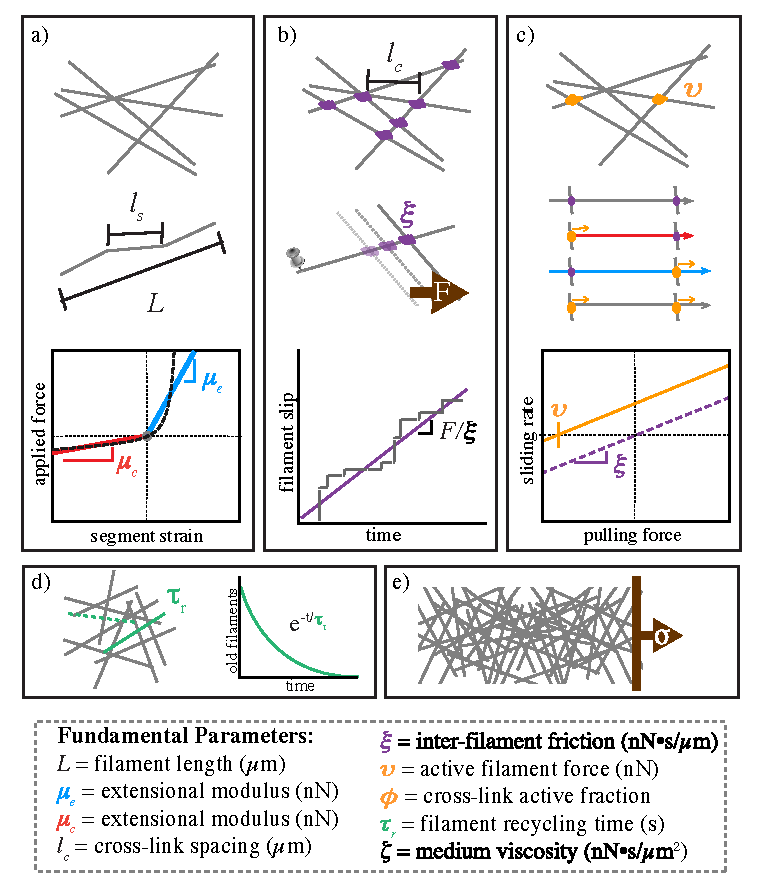
\includegraphics[width=\hsize]{figures/fig2/fig2}
\caption{\label{fig:sim} Schematic of modeling framework. a) Asymmetric filament compliance.Filaments have smaller spring constant for compression than for extension. b) Cross-link slip. Cross-links are coupled by an effective drag, such that their relative motion is
proportional to any applied force. c) Motor activity. Filament activity manifests as a basal sliding rate even in the absence of an external force. Fractional activity. Only a subset of filament cross-links are active, resulting in differential force exertion along the filament. d) Filament recycling. Filaments are turned over at a constant rate, leading to a refreshing in the strain state of all filaments after a characteristic timescale. e) Applied stress. In simulations with passive cross-links, and external stress is applied as force filed acting on a fixed spatial domain.}
\end{figure}

Our motivation is to model essential microscope features of cross-linked actomyosin networks (semi flexible actin filaments with asymmetric compliance, dynamic cross-links, active motors and and continuous filament recycling), in a way that is simple enough to allow systematic exploration of how tuning these microscopic features controls macroscopic network deformation and flow. We focus on 2D networks for computational tractability and because they capture a reasonable approximation of the quasi-2D cortical actomyosin networks that govern flow and deformation in many eukaryotic cells\cite{cellmech_flows, salbreuxbphs}, or the quasi-2D networks used in recent in vitro studies\cite{rheo_2D1,rheo_2D2}.


\subsection*{Asymmetric filament compliance}
We model individual filaments as chains of springs with relaxed length $l_s$.  Filaments can therefore be represented as a sequence of nodes with positions $\mathbf{x_i}$ and nearest neighbor force interactions, $\mathbf{F^{\mu}_i}$, of the form

\begin{equation}
\label{eqn:spring}
\mathbf{F^{\mu}_{i,i+1}} = \mu\frac{|\mathbf{x_{i+1}}-\mathbf{x_i}|-l_s}{l_s}\left ( \frac{\mathbf{x_{i+1}}-\mathbf{x_i}}{l_s}\right )
\end{equation}


where the modulus, $\mu$, is a composite quantity representing both filament and cross-linker compliance in a manner similar to a proposed effective medium theory \cite{theo_crosslinknonlinear}.   To model asymmetric filament compliance, we assign the modulus $\mu$, a different value depending on whether $(|\mathbf{x_{i-1}}-\mathbf{x_i}|-l_s)/l_s$ (the strain) is greater or less than 0. In the limit of highly rigid cross-links and flexible filaments, our model reduces to the pure semi-flexible filament models of \cite{theo_hlm,theo_hlm2}.  In the opposite regime of nearly rigid filaments and highly flexible cross links, our method is still largely similar to the model of \cite{theo_crosslinknonlinear} in small strain regimes before any nonlinear cross link stiffening.  In a departure from those models, we assume here that the magnitude of the force on interior cross-links is the same as those on the exterior.  This approach ignores the variation in strain on these two sets of cross-links as addressed in \cite{theo_crosslinknonlinear}, but we choose to ignore this variation in favor of an approximated, global mean approach.  

Because we are dealing with semi-flexible filaments we also introduce a bending modulus between our filament segments such that the restoring force is proportional to the angle between the filament segments and points in the direction orthogonal to the filament direction, $\mathbf{u_i}=(\mathbf{x_{i-1}}-\mathbf{x_{i}})/|\mathbf{x_{i-1}}-\mathbf{x_{i}}|$.   

\begin{equation}
\label{eqn:bend_spring}
\mathbf{F^{\kappa}_{i-1,i,i+1}} = \frac{\kappa}{l_s} acos \left(\frac{(\mathbf{x_{i+1}}-\mathbf{x_i})\cdot (\mathbf{x_{i-1}}-\mathbf{x_i})}{|\mathbf{x_{i+1}}-\mathbf{x_i}|\cdot |\mathbf{x_{i-1}}-\mathbf{x_i}|}\right)\mathbf{u_i}_\perp
\end{equation}

However, this introduces another mode of asymmetric compliance since filaments under compression are able to bend outward at their centers.  For this reason, in the majority of the work in this paper, we have selected to set $l_s=L$ to simplify away the dependence on bending driven asymmetries.  We show in our supplemental figures (TBA) that the major points of the paper are still valid when we set $l_s<L$ under the condition that $\kappa/l_s\gg\mu_c$.  Therefore, in the majority of the paper we limit our focus to filaments that are constrained not to bend.

Together these forces combine into a single term denoting all the internal forces of the filament mechanics.

\begin{equation}
\label{eqn:internal}
\mathbf{F^{int}_i} = \mathbf{F^{\mu}_{i-1,i}} + \mathbf{F^{\mu}_{i,i+1}} + \mathbf{F^{\kappa}_{i-1,i,i+1}} - \mathbf{F^{\kappa}_{i-2,i-1,i}} - \mathbf{F^{\kappa}_{i,i+1,i+2}}
\end{equation}

\subsection*{Drag-like coupling between overlapping filaments}
\label{exp_drag}
Previous models represent cross-linkers as elastic connections between pairs of points on neighboring filaments that appear and disappear with either fixed or force-dependent probabilities \cite{model_taeyoon,theo_crosslinknonlinear}.  Here, we introduce a simpler coarse-grained model for dynamic cross-links by replacing many transient elastic interactions with an effective drag-like coupling between every pair of overlapping segments.
\begin{equation}
\label{eqn:drag}
\mathbf{F^{\xi}_{i-1,i}} = \xi \sum_j \frac{l_s-|s_{ij}-s_i|}{l_s}  (\mathbf{v_{i-1,i}}-\mathbf{v_{j-1,j}}) 
\end{equation}

where $\mathbf{v_{n-1,n}}$ represent the average velocity of the filament segment stretching between filament node $n-1$ and node $n$, and the sum is taken over all filament segments such that the segment from node $j-1$ to node $j$ intersects the segment from $i-1$ to $i$ at the location $s_{ij}$.  

\begin{equation}
\label{eqn:drag}
\mathbf{F^{coup}_{i}} = \mathbf{F^{\xi}_{i-1,i}} + \mathbf{F^{\xi}_{i,i-1}} 
\end{equation}

This model assumes a linear relation between applied force and the velocity difference between attached segments.  This drag-like coupling has been shown to be an adequate approximation in the case of ionic cross-linking of actin\cite{mol_fric,theo_hydroish2}, and can be found in the theoretical basis of force-velocity curves for myosin bound filaments\cite{theo_frictionShila}. Although non-linearities can arise through force dependent detachment kinetics and/or non-linear force extension of cross-links, we assume that inhomogeneities from non-linear effects are of second or higher order. With this assumption, the motion of filaments can be described by a deterministic dynamical equation of the form

\begin{equation}
\label{eqn:syst1}
0 = -l_s\zeta\mathbf{ v_i} -\mathbf{F^{coup}_i}+ \mathbf{F^{int}_i}
\end{equation}

Here, the first term in the integral is the filament's intrinsic drag through its embedding fluid, $\zeta$, while the second comes from the drag-like coupling between filaments, $\xi$.  

\subsection*{Active coupling for motor driven filament interactions}

To add motor activity we select a subset of cross-linked points and impart an additional force of magnitude $\upsilon$ directed in the orientations of the individual filaments, $\mathbf{u_i}=(\mathbf{x_{i-1}}-\mathbf{x_{i}})/|\mathbf{x_{i-1}}-\mathbf{x_{i}}|$.  This leads to a modification of the equation of motion to

\begin{equation}
\label{eqn:moto}
\mathbf{F^{\upsilon}_{i-1,i}}=\upsilon \mathbf{u_i}\sum_j \frac{l_s-|s_{ij}-s_i|}{l_s}q_{ij}
\end{equation}

where $q_{ij}$ can be 0 or 1 depending on whether there is an ``active'' cross-linker at this location.  In this formulation, only at the subset of points where $q_{ij}=1$ will there be a force imparted.  In our simulations we let $q_{ij}$ be selected randomly such that $\bar{q}=\phi$, where $\bar{q}$ indicates the mean of $q$.



Finally, for each active force, $\mathbf{F^{act}_j}$, imparted by filament $j$, we must also impart the opposite force onto the filament between $i$ and $i+1$ as well.  Therefore, the entire equation for activity will appear as

\begin{equation}
\label{eqn:active}
\mathbf{F^{act}_{i}}=\mathbf{F^{\upsilon}_{i-1,i}} + \mathbf{F^{\upsilon}_{i,i+1}}
- \sum_{j}\mathbf{F^{\upsilon}_{j-1,j}}q_{ij}
\end{equation}


This will leave us with a full equation of motion given by the sum of each of the parts defined above.

\begin{equation}
\label{eqn:syst3}
0=-L\zeta\mathbf{ v_i} -\mathbf{F^{coup}_i}+ \mathbf{F^{int}_i}+\mathbf{F^{act}_i} 
\end{equation}

\subsection*{2D network formation}

We used a mikado model approach \cite{Unterberger2014} to initialize a minimal network of connected unstressed linear filaments in a rectangular 2D domain. We generate 2D networks of these semi-flexible filaments by laying down straight lines of length, L, with random position and orientation. We then assume that overlapping filaments become cross-linked at their points of overlap. Although real cytoskeletal networks may form with non-negligible anisotropy, for simplicity, we focus on isotropically initialized networks. We define the density using the average distance between cross-links along a filament, $l_c$. A simple geometrical argument can then be used to derive the number of filaments filling a domain as a function of $L$ and $l_c$\cite{theo_hlm}.  Here, we use the approximation that the number of filaments needed to tile a rectangular domain of size $D_x \times D_y$  is $2D_xD_y/Ll_c$, and that the length density is therefore simply, $2/l_c$. In the absence of cross-link slip, we expect the network to form a connected solid with a well defined elastic modulus\cite{theo_hlm,theo_hlm2}.


\subsection*{External applied stress}
We can model our active networks as a coupled system of differential equations satisfying \ref{eqn:syst3}.  However, to probe the passive response of the network, we also wish to incorporate externally applied stresses.  Although the general passive mechanical response of this system may be very complex, we focus our attention on low frequency deformations and the steady-state creep response of the system to an applied stress.  To do this we introduce a fixed stress, $\sigma$ along a fixed domain at one edge of the network.  The stress is applied via individual forces to the filaments lying within a patch of size $D_w$ such that the sum of individual forces is equal to the applied stress times the height of the domain.  These forces points in the direction, $\mathbf{\hat{x}}$, producing an extension of the patch.  The region of applied stress does not move as the network deforms, allowing us to more easily focus our attention on a fixed sized domain. 

Finally, we add a 0 velocity constraint at the other edge of our domain of interest.  We assume that our network is in the ``dry,'' low Reynold's number limit, where inertial effects are so small that we can equate our total force to 0.  Therefore, we have a dynamical system of wormlike chain filaments satisfying

\begin{equation}
\label{eqn:systfull}
0=-L\zeta\mathbf{ v_i} -\mathbf{F^{coup}_i}+ \mathbf{F^{int}_i}+\mathbf{F^{act}_i} + \sigma\mathbf{\hat{u}(x_i)}
\end{equation}

subject to constraints such that $\mathbf{v_i(x)}$ is 0 with $x=0$.  This results in an implicit differential equation for filament segments which can be discretized and integrated in time to produce a solution for the motion of the system.


\subsection*{Modeling filament turnover}

In living cells, actin filament assembly is governed by multiple factors that control nucleation, elongation and filament branching. Likewise filament disassembly is governed by multiple factors that promote filament severing and monomer dissociation at filament ends. Here, we focus on a lowest order model for filament recycling in which entire filaments appear with a fixed rate per unit area, $k_{app}$ and disappear at a rate $k_{diss}\rho$, where $\rho$ is a filament density. With this assumption, in the absence of network deformation, the density of filaments will equilibrate to a steady state density, $k_{app}/k_{diss}$, with time constant $\tau_r = 1/k_{diss}$.   In deforming networks, the density will be set by a competition between strain thinning ($\gamma>0$) or thickening ($\gamma<0$), and density equilibration via turnover. To implement this assumption, at fixed time interval $\tau_s < 0.01\cdot\tau_r$ (i.e. 1\% of the equilibration time), we selected a fraction, $\tau_s/\tau_r$, of existing filaments (i.e. less than 1\% of the total filaments) for degradation. We then generated a fixed number of new unstrained filaments $k_{app}\tau_sD_xD_y$ at random positions and orientations within the original domain.   We refer to this continuous turnover as filament recycling, to $k_{diss}=1/\tau_r$ as the recycling rate, and to $\tau_r$ as the recycling time.


\subsection*{Simulation methods}

Details of our simulation approach can be found in the Appendix. Briefly, equations \ref{eqn:spring},\ref{eqn:drag},\ref{eqn:moto} and \ref{eqn:systfull} define a coupled system of ordinary differential equations for the velocities of the endpoints of filament segments, $\mathbf{\dot{x}}$.  These equations are coupled by the effective cross-link friction on segment overlap points, yielding a system of the form:

\begin{equation}
\mathbf{A \cdot \dot x} = \mathbf{f(x)}
\end{equation}

where $\mathbf{A }$ represents a coupling matrix between endpoints of filaments that overlap, and $\mathbf{f(x)}$ is the spring force between pairs of filament segment endpoints.   We numerically integrate this system of equations to find the time evolution of the positions of all filament endpoints. We generate a network of filaments with random positions and orientations as described above within a domain of size $D_x$ by $D_y$.  For all simulations, we imposed periodic boundaries in the y-dimension. To impose an extensional stress, we constrained all filament segment endpoints within a fixed distance $0.05\cdot D_x$ from the left edge of the domain to be non-moving, then we imposed a rightwards force on all segment endpoints within a distance $0.05\cdot D_x$ from the left edge of the patch.   To simulate free contraction, we removed all constraints at boundaries; to assess buildup of contractile stress under isometricc conditions, we pinned both left and right edges of the network as described above.




We smoothed all filament interactions, force fields, and constraints over small regions such that the equations contained no sharp discontinuities. The nominal units for length, force, and time are $\mu m$, nN, and s, respectively.  We explored parameter space around an estimate of biologically relevant parameter values given in Table \ref{table:para}. 

\begin{table}[h]
\centering
\caption{Simulation Parameter Values}
\label{table:para}
\begin{tabular}{|c|c|c|c|c|}
\hline
{\bf parameter}             & {\bf symbol} & {\bf physiological estimate}          \\ \hline
extensional modulus         & $\mu_e$        & $1 nN $                                               \\
compressional modulus             & $\mu_c$     & $ 0.01 nN $                           \\
cross-link drag coefficient & $\xi$      & $unknown $              \\
solvent drag coefficient     & $\zeta$        & $0.0005 \frac{nN s}{\mu m^2} $      \\
filament length             & L            & $5 \mu m$                                          \\
cross-link spacing          & $l_c$        & $0.5 \mu m$                                         \\
domain size                 & $D_x\times D_y$            & $20\times 50 \mu m$                                 \\ \hline
\end{tabular}
\end{table}



% Results and Discussion can be combined.
\section*{Results and Discussion}
We aim to characterize how rates and patterns of cortical flow are shaped by complex dependencies of active stress generation and passive stress dissipation on network architecture, local coupling (active and passive) between filaments and filament recycling.  We approached this in three steps: First, we analyzed the passive deformations of cross-linked networks (absent active motors) in response to a constant external force. Then, we analyzed the dynamics of internal stress buildup and dissipation in the same networks, but with active motors, as they contract freely or build force against fixed external boundaries. Finally, we consider the dynamic interplay of internal stress buildup, contraction, and stress relaxation in networks that undergo steady state flow in response to spatial gradients of motor activity.

% PASSIVE SECTION
\subsection*{Filament recycling prevents cortical tearing and modulates the viscous stress relaxation of passive filament networks}
 
% Example of passive simulation measurements
\paragraph{Networks with passive cross-links and no filament turnover undergo three stages of deformation in response to an extensional force.} 

To characterize the passive response of a cross-linked filament network in the absence of filament recycling and motor activity, we imposed an external force on the simulated network, and then quantified the mechanical response in terms of internal network stress and network strain as a function of time. Figure \ref{fig:passive_ex}a shows the typical response of a simulated network. We measured the local velocity of the network at different positions along the axis of deformation as the mean velocity of all filament segments intersecting that position; we measured the internal network stress at each position by summing the axial component of the tensions on all filament segments intersecting that position, and dividing by network height; finally, we measured network strain rate as the average of all filaments velocities divided by their positions.

During early (not shown) and intermediate (Figure \ref{fig:passive_ex}b) stages of the deformation, the internal stress (blue) was nearly constant throughout the material while the velocity (orange) increased linearly with distance from the site of network attachment, indicating an approximately uniform deformation (strain) rate throughout the material. Accordingly, we report the network response in terms of time-dependent bulk material stress and strain.

Plotting the bulk stress and strain as a function of time revealed that the deformation occurred in three qualitatively distinct phases (Figure \ref{fig:passive_ex}a,c). On short timescales the response was viscoelastic, with a rapid buildup of internal stress and a rapid $\sim$exponential approach to a fixed strain, which represents the elastic limit in the absence of cross-link slip predicted by \cite{theo_hlm}. On intermediate timescales, the internal stress remained constant while the network continued to deform slowly and continuously with nearly constant strain rate (shown as dashed line in Fig \ref{fig:passive_ex}c) as filaments slipped past one another against the effective cross-link drag. This linear relationship between strain and time characterizes a material with an effective viscosity, $\eta$, given by the ratio of the applied stress to the strain rate. We define the transition time between the fast, viscoelastic phase and the slower, effectively viscous deformation phase as $\tau_c$. Finally, as the network strain approached a critical value ($\sim 30\%$ for the simulation in Figure \ref{fig:passive_ex}), strain thinning led to decreased network connectivity, local tearing, and acceleration of the network deformation (see inset in Figure \ref{fig:passive_ex}c), eventually resulting in the highly heterogeneous network structure shown in the t=440s example of Figure \ref{fig:passive_ex}a. 

\begin{figure}[h!]
\centering
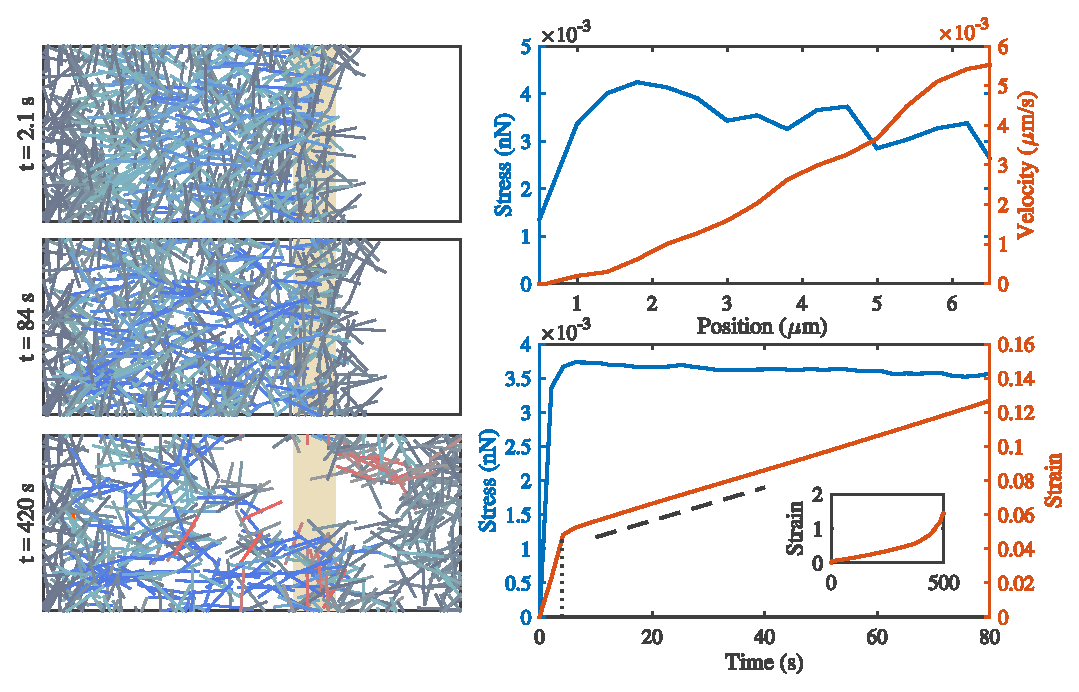
\includegraphics[width=\hsize]{figures/figure3a}
\caption{\label{fig:passive_ex}  Networks with passive cross-links and no filament turnover undergo three stages of deformation in response to an extensional force.   \textbf{a)} Three successive time points from a simulation of a $4\times10\: \mu m$ network deforming under an applied extensional stress of 0.005 $nN/\mu m$ (stress is applied to filaments in the region indicated by the tan bar). In this and all subsequent figures, filaments are color-coded with respect state of stress (blue = tension, red = compression).  Network parameters: $L=1\: \mu m$, $l_c=0.3\: \mu m$, $\xi=100\: nN\cdot s/\mu m$. \textbf{b)} Mean filament stress and velocity profiles for the  network in (a) at t=88s. Note that the stress is nearly constant and the velocity is nearly linear as predicted for a viscous fluid under extension.  \textbf{c)} Plots of the mean stress and strain vs time for the simulation in (a), illustrating the three stages of deformation: (i) A fast initial phase accompanies rapid buildup of internal network stress; (ii) after a characteristic time $\tau_c$ (indicated by vertical dotted line) the network deforms like a material with a constant effective viscosity, $\eta_c$, as indicated by the slope of the dashed line; (iii) at long times, the strain accelerates (see inset) as the network undergoes strain thinning and eventually tears. }
\end{figure}

% Viscosity and timescale parameter dependence
\paragraph{Network architecture sets the rate and timescales of deformation.}  To better understand how network architecture and cross-link dynamics control effective viscosity and the timescale for transition to viscous behavior, we systematically varied network parameters (see \nameref{S1_Table}), and measured the elastic modulus, $G_0$, effective viscosity, $\eta$, and transition time, $\tau_c$, in response to a fixed external stress. We observed the transition from a viscoelastic to an effectively viscous phase for the entire range of parameters that we sampled.  The elastic limit that we observe during the viscoelastic phase agreed closely with the closed form solution for the elastic modulus  $G_0 \sim \mu/l_c$ predicted by a previous model \cite{theo_hlm} for networks of semi-flexible filaments with irreversible cross-links (\nameref{fig:passive_supp}). A simple theoretical analysis (shown in \nameref{S1_Text}) predicts that in the viscous phase, the effective viscosity should be proportional to the cross-link drag coefficient and to the square of the number of cross-links per filament, with a constant of proportionality $\pi/4$. We define this predicted scaling of effective viscoisty as $\eta_c$.

\begin{equation}
\eta_c = \frac{\pi}{4}\xi\left ( \frac{L}{l_c}-1\right )^2
\end{equation}


As shown in Figure \ref{fig:passive_form}a, our simulations agree well with this prediction for a large range of network parameters. For many linear viscoelastic materials, the ratio of the viscosity, $\eta_c$, to the elastic modulus, $G_0$, is a general indicator of the transition timescale from elastic to viscous behavior\cite{mccrum1997principles}. Using our approximations of the elastic modulus and viscosity, we predict a crossover time, $\tau_c \approx L^2\xi/l_c\mu$. By measuring the time at which the strain rate became nearly constant (i.e $\gamma \sim t^n$ with $n>0.8$) we obtained an estimate of this time for a wide variety of simulation parameters. As shown in Figure \ref{fig:passive_form}b, our approximation is in good agreement with the observed transition time, indicating that the passive responses of our simulated networks are well represented by effectively linear bulk properties.


\begin{figure}[h!]
\centering
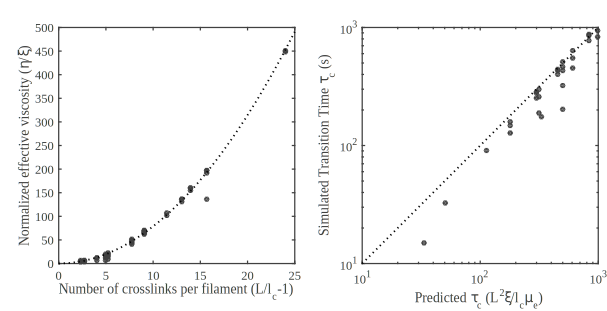
\includegraphics[width=\hsize]{figures/figure3b}
\caption{\label{fig:passive_form} Network architecture sets the rate and timescales of deformation. \textbf{a)} The effective viscosity depends on the drag coefficient and the density of the network. Data points are the normalized effective viscosity from simulations (effective viscosity measured in fluid phase divided by the cross link friction coefficient) vs the number of cross links per filament $(L/l_c - 1)$.  Dotted line indicates the relationship predicted by a simple theory, $\eta_c = \xi(L/l_c-1)^2$ \textbf{b)} The transition to viscous behavior occurs at a characteristic time, $\tau_c$.  }
\end{figure}


% Passive Recycling
\paragraph{Filament recycling rescues network tearing and modulates effective viscosity.} 
 
\begin{figure}[h!]
	\centering
	\includegraphics[width=\hsize]{figures/figure5a}
	\caption{\label{fig:passive_rec}  Filament recycling modulates effective viscosity in two regimes. \textbf{a)} Examples of $20 \times 12 \mu m$ network under 0.001 $nN/\mu m$ extensional stress with recycling ($\tau_r=10 s$) and without, ($\tau_r=\infty$).  Both images are taken when the patches had reached a net strain of 0.4.  The network with recycling doesn't appear to change shape because its components have been recycled to remain in the original domain.  Network parameters: $L=3\: \mu m$, $l_c=0.5\: \mu m$, $\xi=10\: nN\cdot s/\mu m$. \textbf{b)} Strains curves for identical networks with varying levels of filament recycling.  Network parameters: $L=3\: \mu m$, $l_c=0.5\: \mu m$, $\xi=10\: nN\cdot s/\mu m$. \textbf{c)}  Plotting the effective viscosity derived from the slopes of the lines in panel a. The values have been normalized to the predicted effective viscosity. \textbf{d)} Normalized effective viscosities as a function of the normalized recycling time. When the recycling timescale is significantly less than the passive relaxation timescale, the viscosity of the network becomes dependent on recycling time. Red dashed line indicates the approximation given in equation \ref{eqn:simple_eta} for $m=3/4$.}
\end{figure}

To explore how filament recycling shapes the passive network response to an applied force, we ran a series of simulations with identical filament lengths and network densities and cross-link drag coefficients, while varying the filament recycling time $\tau_r=1/k_{diss}$. Figure \ref{fig:passive_rec}a illustrates the results for a particular set of network parameters. In the absence of filament recycling, strain thinning and network tearing lead to a rapid increase in strain rate above a critical strain of $\sim40\%$. 

Progressively decreasing the filament recycling time led to a progressive increase in the rate of network deformation during the effectively viscous phase and an increase in the critical strain at which the network began to tear. Below a critical recycling time ($\tau_{crit}$), the network could sustain effectively viscous deformation indefinitely, as shown by the lack of strain thinning in the strain profiles of Figure\ref{fig:passive_rec}b. Intuitively, steady state deformation is achieved when the rate of filament depletion by strain thinning is balanced by a sufficiently high rate of filament recycling (i.e. a sufficiently low recycling time).  To determine the critical recycling time, we write an equation for the rate of change in filament density $\rho$, as a function of filament recycling ($k_{app}-k_{diss}\rho$) and strain thinning ($-\dot{\gamma}\rho$).
These terms can be rewritten to give the following 

\begin{equation}
\frac{d \rho}{dt} = \frac{\rho_0-\rho}{\tau_r}  - \frac{\sigma}{\eta_c(\rho)} \rho
\end{equation}

where $k_{diss}$  has been replaced by $1/\tau_r$, and $\rho_0 = k_{app}\tau_r$, and $\dot{\gamma}$ has been replaced by $\sigma/\eta_c$.  For our networks, the effective viscosity, $\eta_c$, is dependent on the filament density (through $l_c$) so this dependence must be included. Solving this equation for its steady states, and replacing the initial density, $\rho_0$, with the length density approximation, $1/l_c$, we find that a steady state density only exists under the condition $\tau_r < \tau_{crit}=\eta_c/4\sigma$.  

Reducing recycling time, $\tau_r$, below $\tau_{crit}$ produced different effects on steady state deformation rates depending on the relative values of $\tau_r$ and $\tau_c$, the characteristic time for the transition to effectively viscous deformation in the absence of recycling. For $\tau_r > \tau_c$, the effective viscosity remained $\sim$constant with decreasing $\tau_r$; for $\tau_r < \tau_c$, effective viscosity decreased linearly with decreasing $\tau_r$.  The intuitive explanation for this is as follows: For $\tau_r > \tau_c$, the deformation rate is dominated by cross-link resistance to sliding of strained filaments. For $\tau_r < \tau_c$, the deformation rate is limited by the level of elastic stress on partially strained filaments; By replacing partially strained with unstrained filaments, the network is able to tune the mean level of stress and thus the deformation rate.


To confirm this relationship more generally, we allowed filament lengths, network density and cross link friction to vary more widely, and we measured the network deformation rates while varying filament recycling times (Figure \ref{fig:passive_rec}a,b). We then plotted the normalized effective viscosity (ratio of effective viscosity with recycling to effective viscosity without recycling, $\eta_c$) vs a normalized recycling rate (recycling time scaled by $\tau_c$). Indeed, we found that the normalized effective viscosity measured during steady state flow begins to decrease when the recycling time falls below $\tau_c$ and below this value the effective viscosity falls off nearly linearly with recycling time to minimal values (Figure \ref{fig:passive_rec}c). 

To describe this we introduce (based on linear viscoelastic models of \cite{mccrum1997principles}) an effective recycling viscosity, $\eta_r$, which can be tuned between the $\tau_r$ dependent and independent regimes, depending on the value of the recycling timescale.



\begin{equation}
\label{eqn:simple_eta}
\eta_r = \frac{\eta_c}{1+(\tau_c/\tau_r)^m}  
\end{equation}

For $\tau_r\gg\tau_c$, this simplifies to $\eta_r\approx\eta_c$, while for  $\tau_r\ll\tau_c$, this simplifies to $\eta_r\sim(\tau_r/\tau_c)^k$, which matches with our measurements as found in Figure \ref{fig:passive_rec}d for a large range of parameters (with $m=3/4$). While don't have a clear understanding of where the $3/4$ scaling originates from, this model presents a simple quantitative description of our simulation data.



%Discuss
In summary, we find that tuning recycling times above a critical value $\tau_{crit}$, allows networks to undergo continuous viscous deformation, for long times, without tearing, for a wide range of different effective viscosities and deformation rates. For $\tau_r < tau_{crit}$, modulating filament recycling times can tune the network between two regimes. For $\tau_r > \tau_c$, the deformation is limited by effective cross-link friction, the effective viscosity depends on the strength of inter-filament cross-linking and the network's architecture, and is relatively insensitive to changes in recycling rate. For $\tau_r < \tau_c$, the deformation is governed by the buildup of elastic stress on network filaments, and effective viscosity becomes strongly dependent on recycling time. 

These findings are in agreement with previous simulations on effective viscosity in cross-linked networks. A previous analysis \cite{Kim2014526} looked at the effect of a different form of filament turnover in networks with irreversible cross-linking. The authors also showed two regimes of deformation: one in which network deformation was linearly viscous and tuned by the turnover rate, and one where the creep rate was set purely by the turnover rate independent of applied force.  Although the implementation is different, the two regimes observed in our model are in qualitative agreement and arise from similar microscopic origins. Specifically, the short recycling time regime, where the mechanics are governed by filament extension, is directly equivalent in both models.  For this regime, our model is able to give a theoretical description of the effective viscosity found in \cite{Kim2014526}.  For the opposite regime of long recycling times, the models have a distinct difference.  For the model of \cite{Kim2014526} there was no cross-link unbinding so without of filament turnover, the network would not deform beyond its elastic limit.  In contrast, our simulations always require non-zero cross-link slip so there is always some viscous network deformation.  Therefore, in the regime of long recycling times our model approaches the limit of cross-link dominated viscosity whereas the model of \cite{Kim2014526} approached an infinite viscosity limit.






% ACTIVE SECTION
\subsection*{Filament recycling allows persistent stress buildup in active networks}

\paragraph{In the absence of filament recycling, active networks with free boundaries contract and then stall against passive resistance to network compression.}

\begin{figure}[h!]
	\centering
	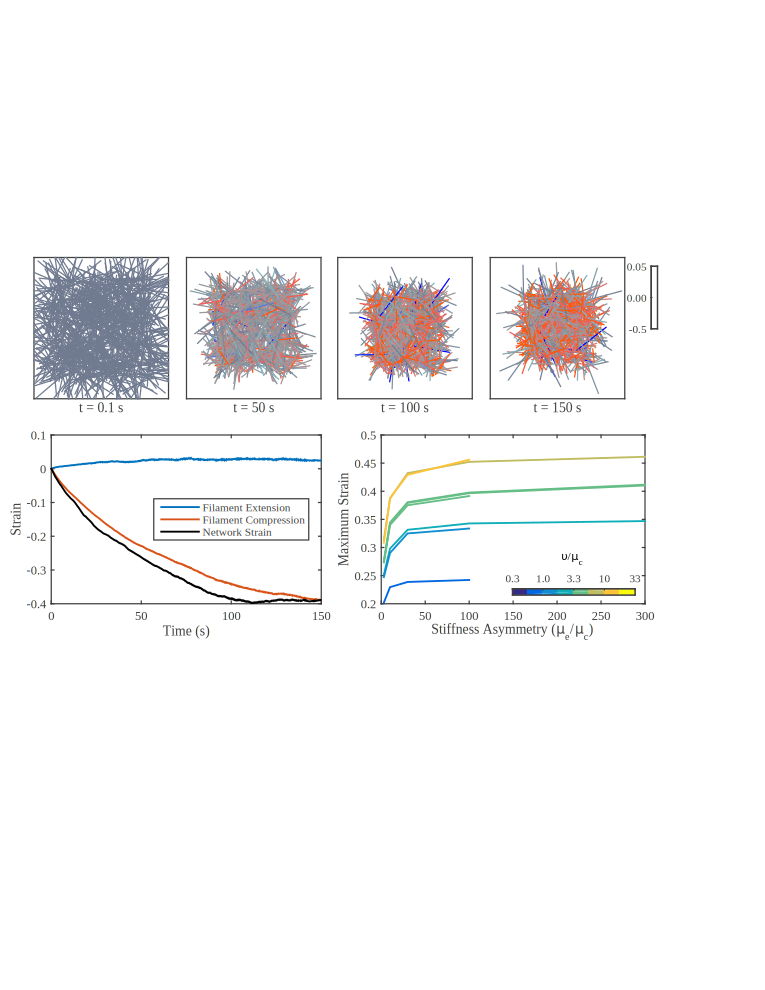
\includegraphics[width=\hsize]{figures/figure4a}
	\caption{\label{fig:active_con} In the absence of filament recycling, active networks with free boundaries contract and then stall against passive resistance to network compression. \textbf{a)}  Example of an active network contracting. Note the buildup of compressive stress as contraction approaches stall between 100 s and 150 s.  Network parameters: $L=5\: \mu m$, $l_c=0.3\: \mu m$, $\xi=100\: nN\cdot s/\mu m$, $\upsilon=0.1\: nN$.  \textbf{b)} Plots showing time evolution of total network strain and  the average extensional (blue) or compressive (red) strain on individual filaments.   \textbf{c)} The network's ability to deform requires asymmetric filament compliance.  Total network strain also increases with the applied myosin force $\upsilon$. Note that the extent of contraction approaches an asymptotic limit as the stiffness asymmetry approaches a ratio of $\sim 100$.}
\end{figure}

Previous theoretical and experimental studies\cite{1367-2630-14-3-033037,rheo_2D1,rheo_active} identified asymmetric filament compliance and dispersion in motor force  as minimal requirements for contraction of disordered networks.To test if our simple implementation of these two requirements (see above) was sufficient to produce macroscopic contraction, we simulated active networks that were unconstrained by external attachments.  Turning on motor activity in an initially unstrained network at $t=0$ produced a rapid initial contraction, followed by a progressive buildup of elastic stress due to compression of individual filaments and an $\sim$exponential approach to stall. On a longer timescale, polarity sorting of individual filaments, as previously described \cite{Ndlec:1997aa,Surrey1167} rearranged the entire network, undoing the initial contraction (see \nameref{active_con_video}).  


We focus here on the contraction phase. During the rapid initial contraction, bulk network strain matched closely the mean compressive strain on individual filaments Figure \ref{fig:active_con}b, Thus  confirming that the origin of bulk contraction in our simulations is filament ?buckling? due to asymmetric filament compliance, as predicted by \cite{1367-2630-14-3-033037,PhysRevX.4.041002} and observed experimentally\cite{rheo_2D1}. Contraction only occurred when the fractional motor activity $0<\phi<1$ (i.e. the fraction of filament intersections with active motors) was less than one, confirming the requirement for dispersion of motor activity (see \nameref{fig:active_supp}) Thus our model effectively captures a minimal mechanism for bulk contractility in disordered networks through asymmetric filament compliance and dispersion of motor activity.

We also determined how microscale parameters shape the rate and final extent of network contraction. Consistent with the idea that contraction stalls when the elastic resistance to filament compression balances the contractile stress., the final extent of contraction increased sharply with motor activity ($\upsilon$) and with the asymmetry in filament stiffness (i.e. the ratio of the extensional and compressive stiffnesses $\mu_e/\mu_c$, Figure \ref{fig:active_con}c,  The time to stall, $\tau_m$, scaled as $L\xi/\upsilon$ (see \nameref{fig:active_supp}b), although the origins of this scaling relationship remain unclear. 


\paragraph{Active networks can only exert a transient force against a fixed boundary in the absence of filament recycling.}

\begin{figure}[h!]
	\centering
	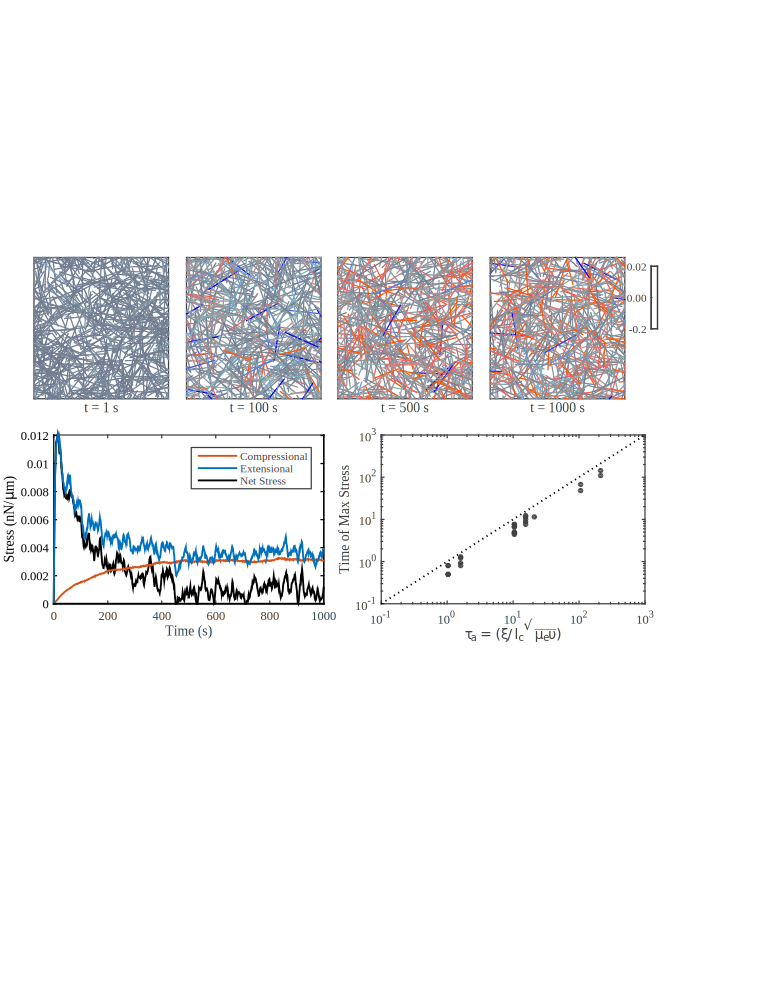
\includegraphics[width=\hsize]{figures/figure4b}
	\caption{\label{fig:active_str} In the absence of filament recycling, active networks can only exert a transient force against a fixed boundary.  \textbf{a)} Simulation of an active network with fixed boundaries illustrating progressive buildup of internal stress through local filament rearrangement and deformation. Note the progressive buildup of compressive stress on individual filaments. Network parameters: $L=5\: \mu m$, $l_c=0.3\: \mu m$, $\xi=100\: nN\cdot s/\mu m$, $\upsilon=0.1\: nN$.  \textbf{b)} Plots of total network stress and the average extensional (blue) and compressive (red) stress on individual filaments for the simulation shown in (a). Rapid buildup of extensional stress allows the network transiently to exert force on its boundary, but this force is dissipated at longer times as   as internal extensional and compressive stresses become balanced. \textbf{c}. Measurement and prediction of the characteristic time ($\tau_a$) at which the maximum stress is achieved. }
\end{figure}

The previous results reveal internal limits on the contraction of networks with free boundaries.  However networks typically build force and contract against an external resistance.  Therefore, we analyzed the buildup and maintenance of contractile stress in active networks contracting against a rigid boundary. We simulated active networks contracting from an initially unstressed state against a fixed boundary Figure \ref{fig:active_str}a, and  quantified the time evolution of mean extensional (blue), compressional (red) and total (black) stress on network filaments \ref{fig:active_str}b. We observed the same qualitative behavior for all network parameters examined: Total stress built rapidly to a peak value $\sigma_a$, and then decayed back to zero again.  The initial rise in total stress was driven by a  rapid buildup of extensional stress, while the decay was caused by a slower dissipation of extensional stress and a comparably slow buildup of compressional stress.  

Sampling these dynamics over a large range of network parameters, we found that the peak stress occurred at a characteristic time, $\tau_a=\xi/l_c\sqrt{\mu\upsilon}$, as shown in Figure \ref{fig:active_str}c. 
{\em Need to say something here about the slower timescale of stress dissipation.  I understand that you have not yet found a scaling relationship for this one.  But it would be very nice, even if you can?t find such a relationship, to have a comparison between  the timescale to reach stall for the freely contracting network and the time to dissipate contractile stress in the pinned case. I.e. is one always bigger than the other for a particular choice of parameters? }

Thus, in the absence of filament turnover, local filament deformation and rearrangement leads to a gradual dissipation of network stress that limits the ability of a network exert sustained force on its boundaries. 


\paragraph{Filament recycling allows networks to exert sustained stress on a fixed boundary.}

\begin{figure}[h!]
	\centering
	\includegraphics[width=\hsize]{figures/figure5b}
	\caption{\label{fig:active_rec} Filament recycling allows network to exert sustained stress on a fixed boundary. \textbf{a)} Snapshots from simulations of active networks with fixed boundaries for different timescales of filament recycling.  Network parameters are the same as in Figure 6. Note that significant remodeling occurs for longer recycling times. \textbf{b)} Plots of net stress exerted by the network on its boundaries for different recycling times; for long-lived filaments, stress is built rapidly, but then dissipates. Increasing filament turnover rates reduces stress dissipation by recycling compressed filaments; however, very short recycling times prevent any stress from being built up in the first place. \textbf{c)} Plotting the steady state stress derived from the long term stress values of the stress in panel b.  \textbf{d)} Normalized steady state stress as a function of normalized recycling time. The steady state stress is set by the timescale at which the network strain is refreshed relative to the timescale at which the max stress is reached. The values have been normalized to the predicted peak stress, $\sigma_a$ in the absence of recycling. Blue dashed line indicates the approximation given in equation \ref{eqn:simple_sigma} for $n=1$.}
\end{figure}

To explore how this limitation could be relieved by filament recycling, we considered an active network contracting against a fixed boundary, using the same parameters as in Figure \ref{fig:active_str}, and systematically varied filament recycling rates. Adding filament recycling produced two general effects: First, as for the passive case, filament recycling could prevent catastrophic tearing by continuously repairing local structural heterogeneities, and by steadily opposing the effects of local strain thinning (see \nameref{fig:tear_supp}). Second, we found that filament recycling resulted in biphasic modulation of the level of steady state stress.

 For the same network parameters as in Figure \ref{fig:active_rec}a and slow filament recycling ($\tau_r = 1000 s$), the network stress peaked rapidly, but then relaxed to a lower value that persisted for times much longer than $\tau_a$. Decreasing recycling time produced a sharp increase in the steady state stress, although the steady state stress remained lower than its peak value.  However, further decreases in recycling time lead to decreases in the steady state stress as well as sharp decreases in the peak stress. Intuitively, this bimodal dependence of steady state stress on recycling rates emerges from continuous replacement of strained with unstrained filaments, combined with the different timescales for buildup of extensional vs compressive filament stress (Figure \ref{fig:active_rec}b). Because extensional stress builds more rapidly than compressive stress, lowering the recycling time $\tau_c$ should increase net stress until $\tau_c$ is approximately equal to $\tau_a$, the time required to build peak stress from an initially unstressed state. For shorter recycling times, the average filament will not have time to build maximum extensional stress before turning over, and thus the steady state stress should decrease with further decreases in $\tau_c$. Plotting normalized steady state stress (steady state stress/peak stress) vs normalized recycling time ($\tau_c$ /$\tau_a$) confirms that this biphasic dependence of steady state stress on recycling times holds for a large range of sampled values for network parameters \ref{fig:active_rec}d.


In the same manner as for the equation of passive response (i.e. Equation \ref{eqn:simple_eta}), we can approximate the dependence of the steady state stress on the filament recycling rate using a simple equation. 

\begin{equation}
\label{eqn:simple_sigma}
\sigma_{ss} = \frac{\sigma_{peak}}{(\tau_r/\tau_a)^n+\tau_a/\tau_r}  
\end{equation}

For $\tau_r\gg\tau_a$, this simplifies to $\sigma_{ss}\sim(\tau_a/\tau_r)^n$, while for $\tau_r\ll\tau_a$, this simplifies to $\sigma_{ss}\sim\tau_r/\tau_a$. What sets the scaling $n$ remains unclear, and this scaling does not appear to be consistent across all simulation setups (Figure \ref{fig:active_rec}d). However, equation \ref{eqn:simple_sigma} still captures a qualitatively correct description of steady state stress in our simulation data.


We repeated the single domain (passive or active) simulations while varying all of our networks microscopic parameters.   By exploring the effect of these parameters on the output variables we were able to determine the general form of the dependence. In Figure \ref{fig:passive_rec}d, we illustrate the data collapse of all our simulation results (see \nameref{S1_Table} for details of parameter exploration).  Interestingly, both the viscosity (in Figure \ref{fig:passive_rec}d) and stress (in Figure \ref{fig:active_rec}d) show changes in behaviors on either side of their respective governing timescales ($\tau_c$ for viscosity and $\tau_a$ for active stress).  Effective viscosity was found to be independent of recycling time until recycling time became of the same order as the elastic to viscous crossover timescale, at which point it decreased with decreasing recycling time.  Similarly, the steady state stress increases with increasing recycling time until it reaches the point of peak stress buildup.  From that point it decreases with increasing recycling time.  Taken together, these effects would suggest a simple predicted flow for a given network setup. 







% COMBINED SECTION
\subsection*{Filament recycling tunes the balance between active stress buildup and viscous stress relaxation to generate flows}

Thus far, we have characterized how filament recycling tunes effective viscosity during passive deformation in response to an externally applied stress the steady state stress produced by an active network against an external resistance.  We next sought to characterize how filament recycling tunes steady flows produced by gradients of motor activity in a region of high motor activity contracts against the passive resistance of a neighboring region with low motor activity.  

\paragraph{Filament recycling allows sustained flows in networks with non-isotropic activity.}

\begin{figure}[h!]
	\centering
	\includegraphics[width=\hsize]{figures/figure6a}
	\caption{\label{fig:flow_ex}  Filament recycling allows sustained flows in networks with non-isotropic activity. \textbf{a)} Example simulations of non-isotropic networks with long ($\tau_r=1000$) and short ($\tau_r=33$) recycling timescales. In these networks the left half of the network is passive while the right half is active.  Network parameters are same as in Figures \ref{fig:active_str} and \ref{fig:active_rec}. Importantly, in all simulations $\tau_a<\tau_c$. \textbf{b)} Graph of strain for identical networks with varying recycling timescales.  With long recycling times, the network stalls; reducing the recycling timescale allows the network to persist in its deformation.  However, for the shortest recycling timescales, the steady state strain begins to slowly return to 0 net motion.  \textbf{c)} Graph of network long-term strain rate as a function of recycling timescale for simulations in a) and b). \textbf{d)} Graph of network long-term strain rate as a function of recycling timescale across a wide range of parameter space.  Note that networks only begin to maintain long-term flows when the recycling time is less than $100\tau_a$. }
\end{figure}

We imposed a continuously asymmetric distribution of motor activity on an initially uniformly dense network of passively cross-linked filaments by allowing a fraction of cross links to be active only in the right half of the simulation domain. Then we examined the time-dependent deformation of the network for a range of different filament recycling times Figure \ref{fig:flow_ex}a. We observed a sharp dependence of steady flow on filament recycling rate Figure \ref{fig:flow_ex}b,c. For very longer recycling times, ($\tau_r=1000 s$, dark blue line), there was a rapid initial deformation (contraction of the active domain and dilation of the passive domain), followed by a slow approach to a steady state flow characterized by slow contraction of the right half-domain and a matching dilation of the left half-domain (see \nameref{fig:combo_prof}).  However, with decreasing filament recycling times, we found the network was able to sustain its deformation and that the long term strain rate rose toward an asymptotic limit (Figure \ref{fig:flow_ex}c).  We repeated these measurements for more network parameters and found that at the shortest recycling timescales measured, we still saw the effective viscosity remaining relatively high, indicating that for sufficiently short recycling times the effective viscosity may approach an asymptotic flow rate (Figure \ref{fig:flow_ex}d).







\paragraph{Filament recycling tunes the magnitudes of both effective viscosity and steady state stress.}  


\begin{figure}[h!]
	\centering
	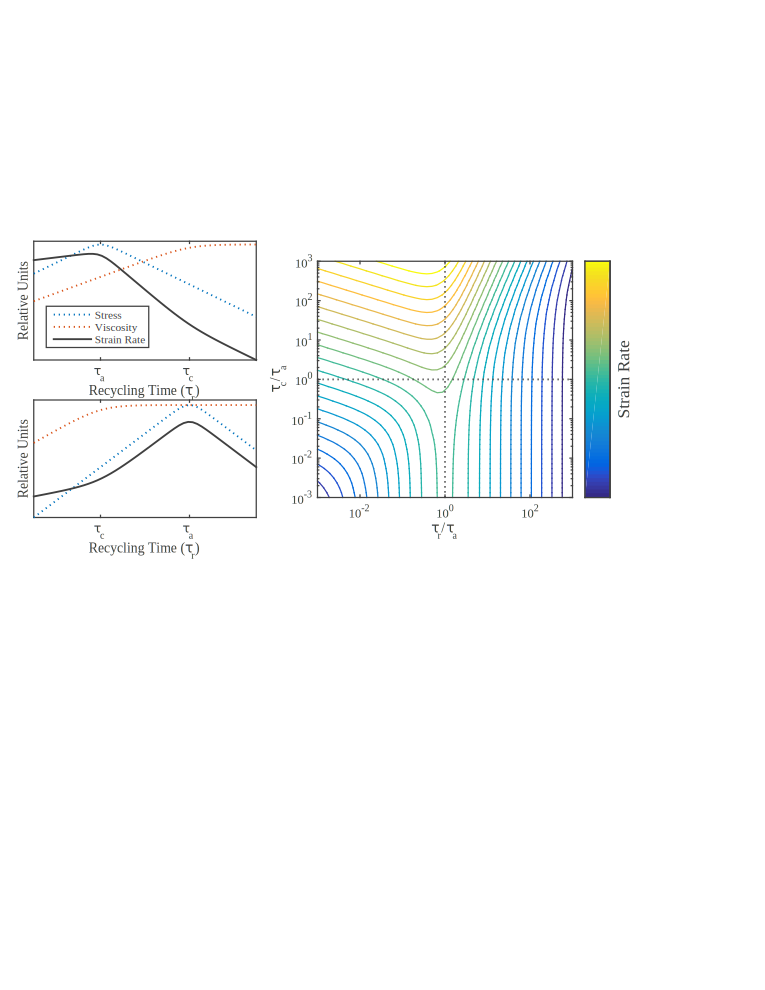
\includegraphics[width=\hsize]{figures/figure_theor}
	\caption{\label{fig:flow_theo}  Filament recycling tunes the magnitudes of both effective viscosity and steady state stress. \textbf{a)}  Dependence of steady state stress and effective viscosity on recycling time $\tau_r$ under the condition $\tau_c<\tau_a$. \textbf{b)} Same as a), but for the case where $\tau_a<\tau_c$.  \textbf{c,d)} Resulting strain rates for network as a function of recycling time $\tau_r$ for the regimes in panels a and b..  }
\end{figure}

This dependence of steady state deformation (flow) rate on filament recycling times can be understood in terms of our previous findings.  During steady state flow, active contraction of the right half-domain is limited both by internal resistance to compression of filaments within the right half-domain (Figure 5), and by passive resistance of the left-half domain (Figure 4).  

Monitoring these two forms of resistance as a function of filament recycling time for the simulations in Figure 8, we see that resistance to compression of filaments in the right half domain makes a significant contribution only for very low recycling rates.  This is again because compressional resistance on filaments in the contracting right half domain takes longer to build than extensional resistance on filaments in the dilating right half-domain. As a consequence, except for very low recycling rates,  steady state deformation is governed by an equation of the form:

\begin{equation}
\label{eqn:simple_sigma}
\dot{\gamma} = \frac{\sigma_{ss}}{\eta_r}  
\end{equation}

where $\sigma_{ss}$ is the active stress generated by the right half-domain (less the internal resistance to filament compression), $\eta_r$ is the effective viscosity of the left half domain and strain rate is measured in the left half-domain.  Therefore, we can understand the dependence of network flow (i.e. strain rate) on filament recycling time $\tau_r$ in terms of the previously characterized dependencies of effective viscosity and steady state stress on $\tau_r$ (Figures \ref{fig:passive_rec}d and \ref{fig:active_rec}d). In particular, recall that there is a transition in the dependence of $\eta_r$ on $\tau_r$ at the characteristic time $\tau_c$, and a transition in the dependence of sigma on $\tau_r$ at the characteristic time $\tau_a$.  Thus, as shown in Figure \ref{fig:flow_theo},  there are two qualitatively distinct cases for the dependence of strain rate on $\tau_r$, depending on the relative magnitudes of $\tau_a$ and $\tau_c$.  For both cases, we expect an increase in strain rate with filament recycling at long recycling times (where effective viscosity is insensitive to strain rate)  and approach to an asymptotic strain rate at low recycling times, where both $\eta_r$ and $\sigma_{ss}$ fall off with different scalings. For $\tau_a < \tau_c$, we predict a peak strain rate at intermediate recycling times followed by a rapid falloff at lower recycling times, whereas for $\tau_a > \tau_c$, we expect a more rapid approach to maximum strain rate and a slower fall off at lower recycling times.  As shown in Figure \ref{fig:flow_theo}d, for the range of network parameters we sampled, the dependence of strain rate on $\tau_r$ is monotonic and approaches an asymptote at low recycling times (i.e. high recycling rates).  This is to be expected because all the parameter values sampled (selected for physiological relevance) satisfied the condition $\tau_a > \tau_c$.



\paragraph{Filament recycling influences architectural control of flow rate.}

\begin{figure}[h!]
	\centering
	\includegraphics[width=\hsize]{figures/figure6b}
	\caption{\label{fig:flow_form}  Filament recycling influences architectural control of flow rate. \textbf{a)}  For a fixed filament recycling time, filament length tuned network deformation rate.  \textbf{b)} Recycling rate is independent of cross-link spacing in this parameter space.}
\end{figure}

Finally, we examined how steady state flow depends on other network parameters when filament recycling rates are held constant.   Interestingly, we found that flow rates are largely insensitive to cross link density ($l_c$) but vary inversely with filament length. Thus, in this region of parameter space, steady state flows may be buffered intrinsically against some forms of variation in network architecture.










%Conclusion
\section*{Conclusion}
Our work aimed to create a simulation framework that would allow us to analyze the origins of macroscopic flow in terms of a handful of physiologically relevant microscopic parameters.  Toward this aim we developed a minimalist model of a 2D filament network and analyzed the network's reaction to a variety of situations.  We found mathematical relationships that determined both the passive effective viscosity and the active stress generation of networks with and without recycling.  From these relationships we were able to make predictions about the rates of network flow in non-isotropic networks mimicking those found in polarized eukaryotic actomyosin cortices.  

Importantly, our work brings a theoretical understanding to the importance of actomyosin turnover in producing and maintaining long-term large scale flows.  We propose the concept of "filament recycling" to refer to the multitude of biochemical interactions which can give rise to the piece by piece architectural resetting of filament networks.  We believe that our analysis of networks in the presence of this filament recycling will be useful in further developing the qualitative and quantitative understanding the deformation of these complex networks.

\section*{Supporting Information}

% Include only the SI item label in the subsection heading. Use the \nameref{label} command to cite SI items in the text.
\paragraph*{S1 Text.}
\label{S1_Text}
{\bf Bold the title sentence.} Add descriptive text after the title of the item (optional).

\paragraph*{S1 Fig.}
\label{S1_Fig}
{\bf Bold the title sentence.} Add descriptive text after the title of the item (optional).

\paragraph*{S2 Fig.}
\label{fig:passive_supp}
{\bf  Mechanical properties of passive networks.}  \textbf{a)} Elastic modulus of networks.  Our measurements closely match prediction of $G_0\sim\mu/l_c$.  \textbf{b)}  Placeholder for inevitably another figure relevant to passive properties..

\paragraph*{S3 Fig.}
\label{fig:tear_supp}
{\bf Mechanical properties of active networks } Add descriptive text after the title of the item (optional).

\paragraph*{S4 Fig.}
\label{fig:active_supp}
{\bf Mechanical properties of active networks } Add descriptive text after the title of the item (optional).

\paragraph*{S6 Fig.}
\label{fig:combo_prof}
{\bf Spatial velocity profile of networks containing passive and active domains.} 

\paragraph*{S1 Table.}
\label{S1_Table}
{\bf Parameter values.}  List of parameter values used for each set of experiments.

\paragraph*{S1 Video.}
\label{passive_ex_video}
{\bf Extensional strain in passive networks.}  Movie of simulation setup shown in Figure \ref{fig:passive_ex}

\paragraph*{S2 Video.}
\label{active_con_video}
{\bf Active networks contracting with free boundaries.}  Movie of simulation setup shown in Figure \ref{fig:active_con}

\section*{Acknowledgments}
We would like to thank Shiladitya Banerjee and Patrick McCall for stimulating discussions.

\nolinenumbers

%\section*{References}
% Compile your BiBTeX database using our plos2015.bst
% style file and paste the contents of your .bbl file
% here.
% 
\bibliographystyle{plos2015}
\bibliography{slippage,active}



\end{document}


% Template for PLoS
% Version 3.1 February 2015
%
% To compile to pdf, run:
% latex plos.template
% bibtex plos.template
% latex plos.template
% latex plos.template
% dvipdf plos.template
%
% % % % % % % % % % % % % % % % % % % % % %
%
% -- IMPORTANT NOTE
%
% This template contains comments intended 
% to minimize problems and delays during our production 
% process. Please follow the template instructions
% whenever possible.
%
% % % % % % % % % % % % % % % % % % % % % % % 
%
% Once your paper is accepted for publication, 
% PLEASE REMOVE ALL TRACKED CHANGES in this file and leave only
% the final text of your manuscript.
%
% There are no restrictions on package use within the LaTeX files except that 
% no packages listed in the template may be deleted.
%
% Please do not include colors or graphics in the text.
%
% Please do not create a heading level below \subsection. For 3rd level headings, use \paragraph{}.
%
% % % % % % % % % % % % % % % % % % % % % % %
%
% -- FIGURES AND TABLES
%
% Please include tables/figure captions directly after the paragraph where they are first cited in the text.
%
% DO NOT INCLUDE GRAPHICS IN YOUR MANUSCRIPT
% - Figures should be uploaded separately from your manuscript file. 
% - Figures generated using LaTeX should be extracted and removed from the PDF before submission. 
% - Figures containing multiple panels/subfigures must be combined into one image file before submission.
% For figure citations, please use "Fig." instead of "Figure".
% See http://www.plosone.org/static/figureGuidelines for PLOS figure guidelines.
%
% Tables should be cell-based and may not contain:
% - tabs/spacing/line breaks within cells to alter layout or alignment
% - vertically-merged cells (no tabular environments within tabular environments, do not use \multirow)
% - colors, shading, or graphic objects
% See http://www.plosone.org/static/figureGuidelines#tables for table guidelines.
%
% For tables that exceed the width of the text column, use the adjustwidth environment as illustrated in the example table in text below.
%
% % % % % % % % % % % % % % % % % % % % % % % %
%
% -- EQUATIONS, MATH SYMBOLS, SUBSCRIPTS, AND SUPERSCRIPTS
%
% IMPORTANT
% Below are a few tips to help format your equations and other special characters according to our specifications. For more tips to help reduce the possibility of formatting errors during conversion, please see our LaTeX guidelines at http://www.plosone.org/static/latexGuidelines
%
% Please be sure to include all portions of an equation in the math environment.
%
% Do not include text that is not math in the math environment. For example, CO2 will be CO\textsubscript{2}.
%
% Please add line breaks to long display equations when possible in order to fit size of the column. 
%
% For inline equations, please do not include punctuation (commas, etc) within the math environment unless this is part of the equation.
%
% % % % % % % % % % % % % % % % % % % % % % % % 
%
% Please contact latex@plos.org with any questions.
%
% % % % % % % % % % % % % % % % % % % % % % % %

\documentclass[10pt,letterpaper]{article}
\usepackage[top=0.85in,left=2.75in,footskip=0.75in]{geometry}

% Use adjustwidth environment to exceed column width (see example table in text)
\usepackage{changepage}

% Use Unicode characters when possible
\usepackage[utf8]{inputenc}

% textcomp package and marvosym package for additional characters
\usepackage{textcomp,marvosym}

% fixltx2e package for \textsubscript
\usepackage{fixltx2e}

% amsmath and amssymb packages, useful for mathematical formulas and symbols
\usepackage{amsmath,amssymb}

% cite package, to clean up citations in the main text. Do not remove.
\usepackage{cite}

% Use nameref to cite supporting information files (see Supporting Information section for more info)
\usepackage{nameref,hyperref}

% line numbers
\usepackage[right]{lineno}

% ligatures disabled
\usepackage{microtype}
\DisableLigatures[f]{encoding = *, family = * }

% rotating package for sideways tables
\usepackage{rotating}

\usepackage{verbatim}   % useful for program listings

% Remove comment for double spacing
%\usepackage{setspace} 
%\doublespacing

% Text layout
\raggedright
\setlength{\parindent}{0.5cm}
\textwidth 5.25in 
\textheight 8.75in

% Bold the 'Figure #' in the caption and separate it from the title/caption with a period
% Captions will be left justified
\usepackage[aboveskip=1pt,labelfont=bf,labelsep=period,justification=raggedright,singlelinecheck=off]{caption}

% Use the PLoS provided BiBTeX style
% \bibliographystyle{plos2015}
\bibliographystyle{apalike}

% Remove brackets from numbering in List of References
\makeatletter
\renewcommand{\@biblabel}[1]{\quad#1.}
\makeatother

% Leave date blank
\date{}

% Header and Footer with logo
\usepackage{lastpage,fancyhdr,graphicx}
\usepackage{epstopdf}
\pagestyle{myheadings}
\pagestyle{fancy}
\fancyhf{}
\lhead{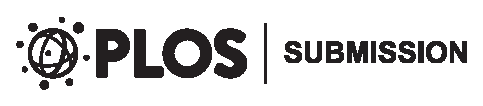
\includegraphics[width=2.0in]{PLOS-submission.eps}}
\rfoot{\thepage/\pageref{LastPage}}
\renewcommand{\footrule}{\hrule height 2pt \vspace{2mm}}
\fancyheadoffset[L]{2.25in}
\fancyfootoffset[L]{2.25in}
\lfoot{\sf PLOS}

%% Include all macros below

\newcommand{\lorem}{{\bf LOREM}}
\newcommand{\ipsum}{{\bf IPSUM}}

%% END MACROS SECTION


\begin{document}

\subsection{Steady-state Approximation of Effective Viscosity}
\label{sec:eff_vic}
We begin with a calculation of a strain rate estimate of the effective viscosity for a network described by our model in the limit of highly rigid filaments.  We carry this out by assuming we have applied a constant stress along a transect of the network.  With moderate stresses, we assume the network reaches a steady state affine creep. In this situation, we would find that the stress in the network exactly balances the sum of the drag-like forces from cross-link slip.  So for any transect of length D, we have a force balance equation.

\begin{equation}
\mathbf{\sigma} = \frac{1}{D}\sum_{filaments}\: \sum_{crosslinks}\xi \cdot (\mathbf{v_i(x)}-\mathbf{v_j(x)})
\end{equation}

where $\mathbf{v_i(x)}-\mathbf{v_j(x)}$ is the difference between the velocity of a filament, $i$, and the velocity of the filament, $j$, to which it is attached at the cross-link location, $\mathbf{x}$. We can convert the sum over cross-links to an integral over the length using the average density of cross-links, $1/l_c$ and invoking the assumption of (linear order) affine strain rate, $\mathbf{v_i(x)}-\mathbf{v_j(x)}=\dot \gamma x$. This results in

\begin{multline}
\mathbf{\sigma} =  \frac{1}{D}\sum_{filaments}\:  \int_0^L \xi \cdot  \: (\mathbf{v_i(s)}-\mathbf{v_j(s)}) \:\frac{ds \cos \theta }{l_c} \\
 = \sum_{filaments}\:  \frac{\xi \dot \gamma L}{l_c} \cos \theta \cdot (x_l + \frac{L}{2} \cos \theta)
\end{multline}

Here we have introduced the variables $x_l$, and $\theta$ to describe the leftmost endpoint and the angular orientation of a given filament respectively.  Next, to perform the sum over all filaments we convert this to an integral over all orientations and endpoints that intersect our line of stress. We assume for simplicity that filament stretch and filament alignment are negligible in this low strain approximation.  Therefore, the max distance for the leftmost endpoint is the length of a filament, L, and the maximum angle as a function of endpoint is $\arccos(x_l/L)$.  The linear density of endpoints is the constant $D/l_cL$ so our integrals can be rewritten as this density over $x_l$ and $\theta$ between our maximum and minimum allowed bounds.

\begin{equation}
\mathbf{\sigma} =  \frac{1}{D} \int_0^L dx_l \int_{-\arccos (\frac{x_l}{L})}^{\arccos (\frac{x_l}{L})}\pi d\theta \frac{\xi \dot \gamma L}{l_c} \cdot \frac{D}{Ll_c}\cdot (x_l \cos \theta + \frac{L}{2} cos^2\theta)
\end{equation}

Carrying out the integrals and correcting for dangling filament ends leaves us with a relation between stress and strain rate.

\begin{equation}
\mathbf{\sigma} = 4 \pi \left ( \frac{ L}{l_c}-1 \right)^2 \xi \dot \gamma 
\end{equation}

We recognize the constant of proportionality between stress and strain rate as a viscosity (in 2 dimensions).  Therefore, our approximation for the effective viscosity, $\eta_{c}$, at steady state creep in this low strain limit is

\begin{equation}
\label{lin_eqn}
\mathbf{\sigma} = 4 \pi \left ( \frac{ L}{l_c}-1 \right)^2 \xi
\end{equation}



\subsection{Critical filament lifetime for steady state filament extension}
We seek to determine a critical filament lifetime, $\tau_{crit}$ , below which the density of filaments approaches a stable steady state under constant extensional strain. To this end, let $\rho$ be the filament density (i.e. number of filaments per unit area). We consider a simple coarse grained model for how $\rho$ changes as a function of filament assembly $k_{ass}$, filament disassembly $k_{diss}$, $\rho$ and strain thinning $\dot{\gamma}\rho$. Using $\rho_0 = \frac{k_{ass}}{k_{diss}}$, $\tau_r=\frac{1}{k_{diss}}$, and $\dot{\gamma}=\frac{\sigma}{\eta_c}$.

\begin{equation}
\label{drho_1}
\frac{d\rho}{dt}=\frac{1}{\tau_r}\left ( \rho_0 - \rho - \frac{\sigma \tau_r}{\eta_c(\rho)} \rho\right )
\end{equation}

where $\eta_c = \eta_c(\rho)$ on the right hand side reflects the dependence of effective viscosity on network density.  The strength of this dependence determines whether there exists a stable steady state, representing continuous flow.  Using $\eta_c(\rho)\sim \xi \left ( \frac{L}{l_c(\rho)} -1 \right )^2$ from above (ignoring the numerical prefactor) and $\rho \sim \frac{2}{L l_c(\rho)}$, we obtain:


\begin{equation}
\label{drho_2}
\frac{d\rho}{dt}=\frac{1}{\tau_r}\left ( \rho_0 - \rho - \frac{\sigma \tau_r}{\xi(\rho L^2/2 -1)^2}\rho\right )
\end{equation}

\begin{figure}[h!]
	\centering
	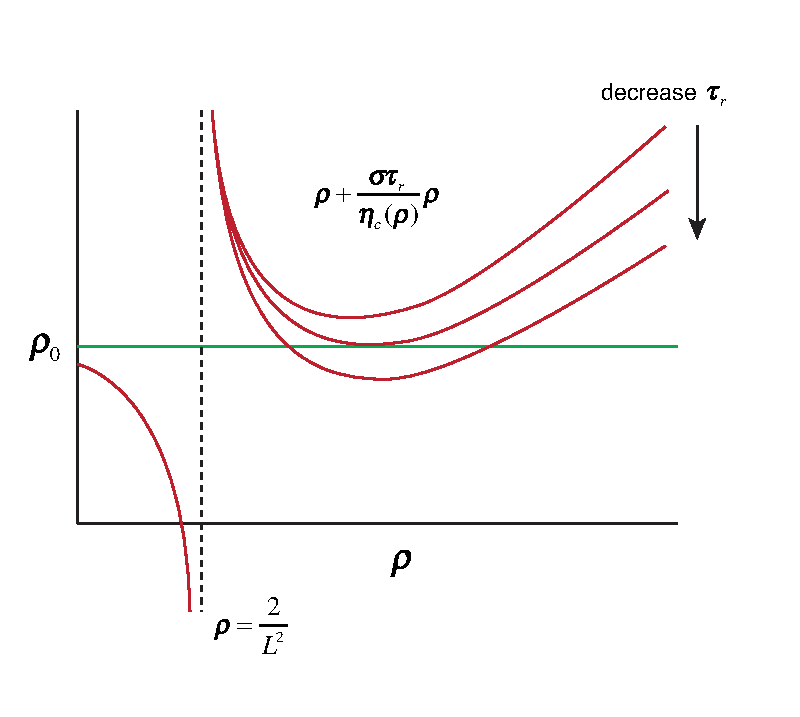
\includegraphics[width=\hsize]{figures/figureS1}
	\caption{\label{fig:flux_balance}  Flux balance analysis of network density. Qualitative plots of $\rho+\frac{\sigma \tau_r}{\eta_c(\rho)}\rho$ (red curves) vs $\rho_0$ (green line) for different values of $\tau_r$.  For sufficiently large $\tau_r$, there are no crossings.  For $\tau_r < \tau_{crit}$, there are two crossings:  The rightmost crossing represents a stable steady state.  }
\end{figure}


Figure \ref{fig:flux_balance} sketches the positive ($\rho_0$) and negative ($\rho+\frac{\sigma \tau_r}{\eta_c(\rho)}\rho$) contributions to the right hand side of Equation 6 for different values of $\tau_r$. For sufficiently large $\tau_r$, there is no stable state, i.e. strain thinning will occur.  However, as $\tau_r$ deceases below a critical value $\tau_{crit}$, a stable steady state appears.  Note that when $\tau_r = \tau_{crit}$, $\rho+\frac{}{den}\rho$ passes through a minimum value $\rho_0$ at $\rho=\rho^*$.  Accordingly, to determine $\tau_{crit}$, we solve:

\begin{equation}
\label{drho_3}
0 = \frac{d}{d\rho}\left( \rho + \frac{\sigma\tau_r}{\eta_c(\rho)} \rho\right ) = 1 - \frac{\sigma\tau_r}{\xi (\rho L^2/2-1)^3}
\end{equation}

From this, with some algebra, we infer that

\begin{equation}
\label{drho_4}
\rho^* = \frac{2}{L^2}\left ( 1 + \left( \frac{\sigma\tau_r}{\xi}\right )^{1/3} \right )
\end{equation}

and 

\begin{equation}
\label{drho_5}
\frac{\sigma\tau_r}{\eta_c(\rho^*)} =  \left( \frac{\sigma\tau_r}{\xi}\right )^{1/3} 
\end{equation}

We seek a value for $\tau_r=\tau_{crit}$ at which


\begin{equation}
\label{drho_6}
\rho^* + \frac{\sigma\tau_{crit}}{\eta_c(\rho^*)}\rho^* =  \rho_0
\end{equation}

Substituting from above, and using $\rho_0=\frac{2}{L l_c}$, we have:

\begin{equation}
\label{drho_7}
\frac{2}{L^2}\left ( 1 + \left( \frac{\sigma\tau_{crit}}{\xi}\right )^{1/3}  \right )
\left ( 1 + \left( \frac{\sigma\tau_{crit}}{\xi}\right )^{1/3}  \right )
= \frac{2}{L l_c}
\end{equation}

Finally, rearranging terms, we obtain

\begin{equation}
\label{drho_8}
\tau_{crit}=\frac{\xi}{\sigma}\left( \sqrt{\frac{L}{l_c}}-1\right )^3
\end{equation}

\subsection{Simulation and Analysis Code Available Online}
All of the simulation and analysis code for generating the figures in this paper is available online.  To find the source code please visit our Github repository at 

https://github.com/wmcfadden/activnet



\begin{table}[h]
\begin{adjustwidth}{-2.25in}{0in}
\centering
\caption{Simulation Parameter Values}
\label{table:para2}
\begin{tabular}{|c|ccccccc|}
	\hline
	Parameter     & \textbf{Figure 3}          & \textbf{Figure 4}       & \textbf{Figure S2a,b}    & \textbf{Figure S2c,d}     & \textbf{Figure 7}    & \textbf{Figure 9}          \\ \hline
	$L$           & $1,3,5,7,10$      & $3$             & $3,5$         & $3,5$                 & $5$         & $3,5,8$            \\ 
	$l_c$         & $0.2,0.3,0.5,0.8$ & $0.3,0.5$       & $0.3$       & $0.15,0.2,0.3,0.4$ & $0.2,0.3$        & $0.15,0.2,0.3,0.4$ \\ 
	$\mu_e/\mu_c$ & $100$             & $100$           & $3-300$     & $100$     & $100$           & $100$              \\ 
	$\mu_c$       & $0.01$            & $0.01$          & $0.01-0.3$  & $0.001-0.03$       & $0.01$      & $0.01$             \\ 
	$\xi$         & $0.1,1$          & $0.05,0.1,1$      & $0.01,0.1,1$  & $0.1,1$  & $0.1,1,3.3$   & $0.1,1$           \\ 
	$\upsilon$    & ~                 & ~               & $0.1,0.3,1$ & $0.1,1$   & $0.1,1,3$    & $0.1$              \\ 
	$\phi$        & ~                 & ~               & $0.25$      & $0.5$     & $0.25,0.75$    & $0.25$             \\ 
	$\tau_r$      & ~                 & $0.1-10^4$      & ~           & ~         & $0.01-10^3$  & $0.01-10^3$              \\ 
	$\sigma$      & $0.0002-0.01$     & $0.00003-0.005$ & ~           & ~         & ~            & ~                          \\
	\hline
\end{tabular}
\end{adjustwidth}
\end{table}

\begin{figure}[h!]
\centering
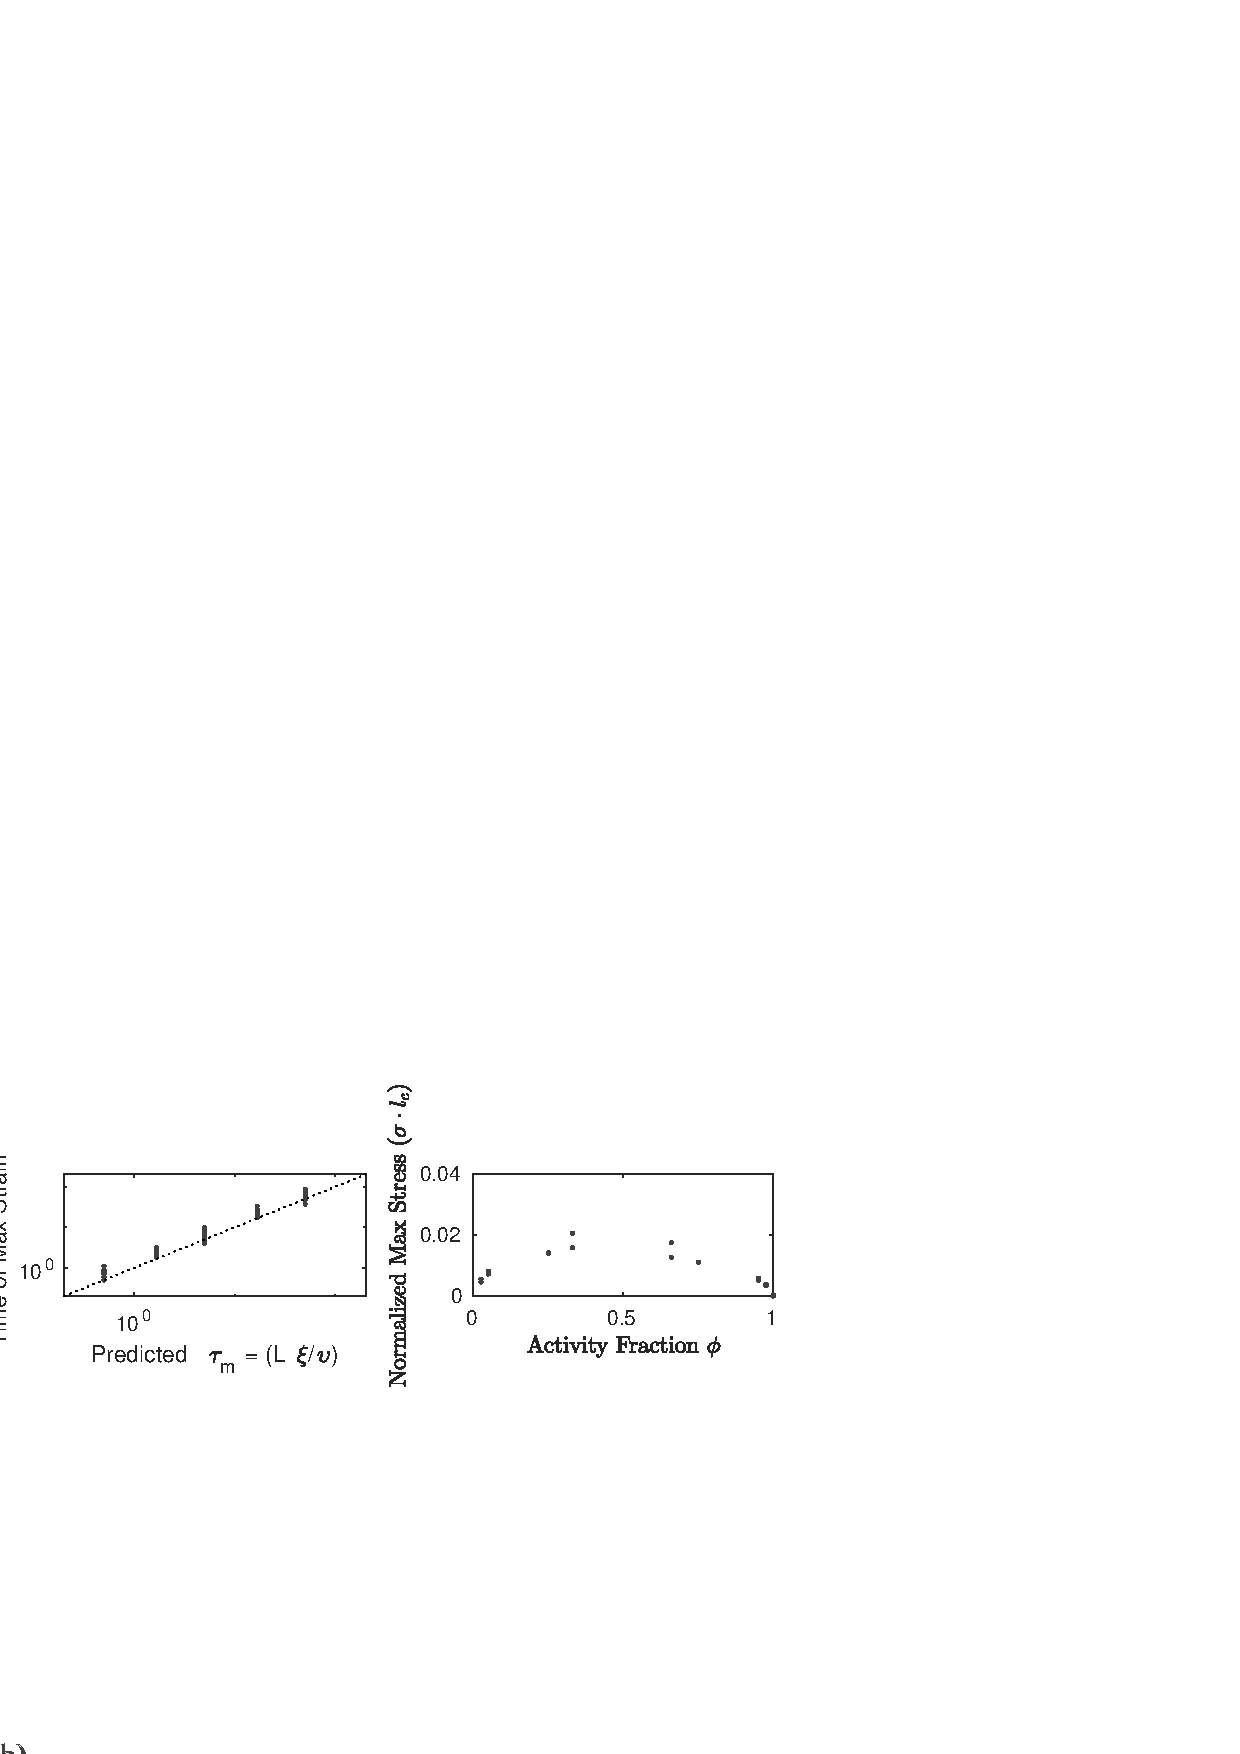
\includegraphics[width=\hsize]{figures/figureS2}
\caption{\label{fig:passive_supp}  Fast viscoelastic response to extensional stress. Plots of normalized strain vs time during the elastic phase of deformation in passive networks under extensional stress.  Measured strain is normalized by the equilibrium strain predicted for a network of elastic filaments without crosslink slip $\gamma_{eq} = \sigma/G_0 = \sigma/(2\mu/l_c)$.  }
\end{figure}

\begin{figure}[h!]
	\centering
	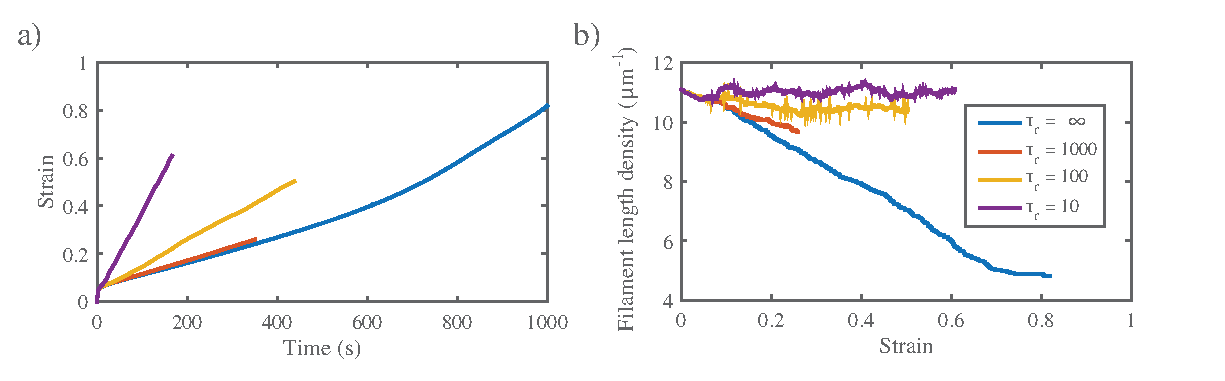
\includegraphics[width=\hsize]{figures/figureS3}
	\caption{\label{fig:thinning}  Filament turnover rescues strain thinning.  \textbf{a)} Plots of strain vs time for different turnover times (see inset in (b)). Note the increase in strain rates with decreasing turnover time. \textbf{b)} Plots of filament density vs strain for different turnover times $\tau_r$.  For intermediate $\tau_r$, simulations predict progressive strain thinning, but at a lower rate than in the complete absence of recycling. For higher $\tau_r$, densities approach steady state values at longer times.  }
\end{figure}

\begin{figure}[h!]
\centering
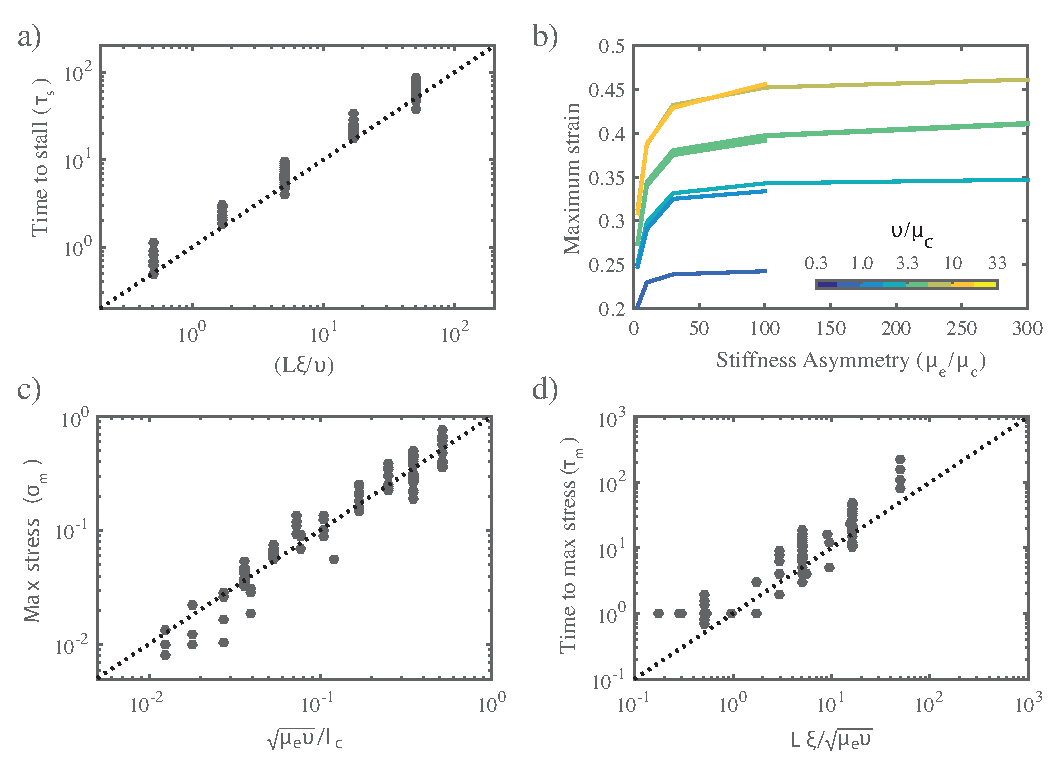
\includegraphics[width=\hsize]{figures/figureS4}
\caption{\label{fig:active_supp}  Mechanical properties of active networks.  \textbf{a)}  Time for freely contracting networks to reach maximum strain, $\tau_s$, scales with $L\xi/\upsilon$.  \textbf{b)} Free contraction requires asymmetric filament compliance, and total network strain increases with the applied myosin force $\upsilon$. Note that the maximum contraction approaches an asymptotic limit as the stiffness asymmetry approaches a ratio of $\sim 100$.   \textbf{c)}  Maximum stress achieved during isometric contraction, $\sigma_m$, scales approximately with $\sqrt{\mu_e\upsilon}/l_c$.  \textbf{d)} Time to reach max stress during isometric contraction scales approximately with $L\xi/\sqrt{\mu_e\upsilon}$. Scalings for $\tau_s$, $\sigma_m$ and $\tau_m$ were determined empirically by trial and error, guided by dimensional analysis. }
\end{figure}

\begin{figure}[h!]
\centering
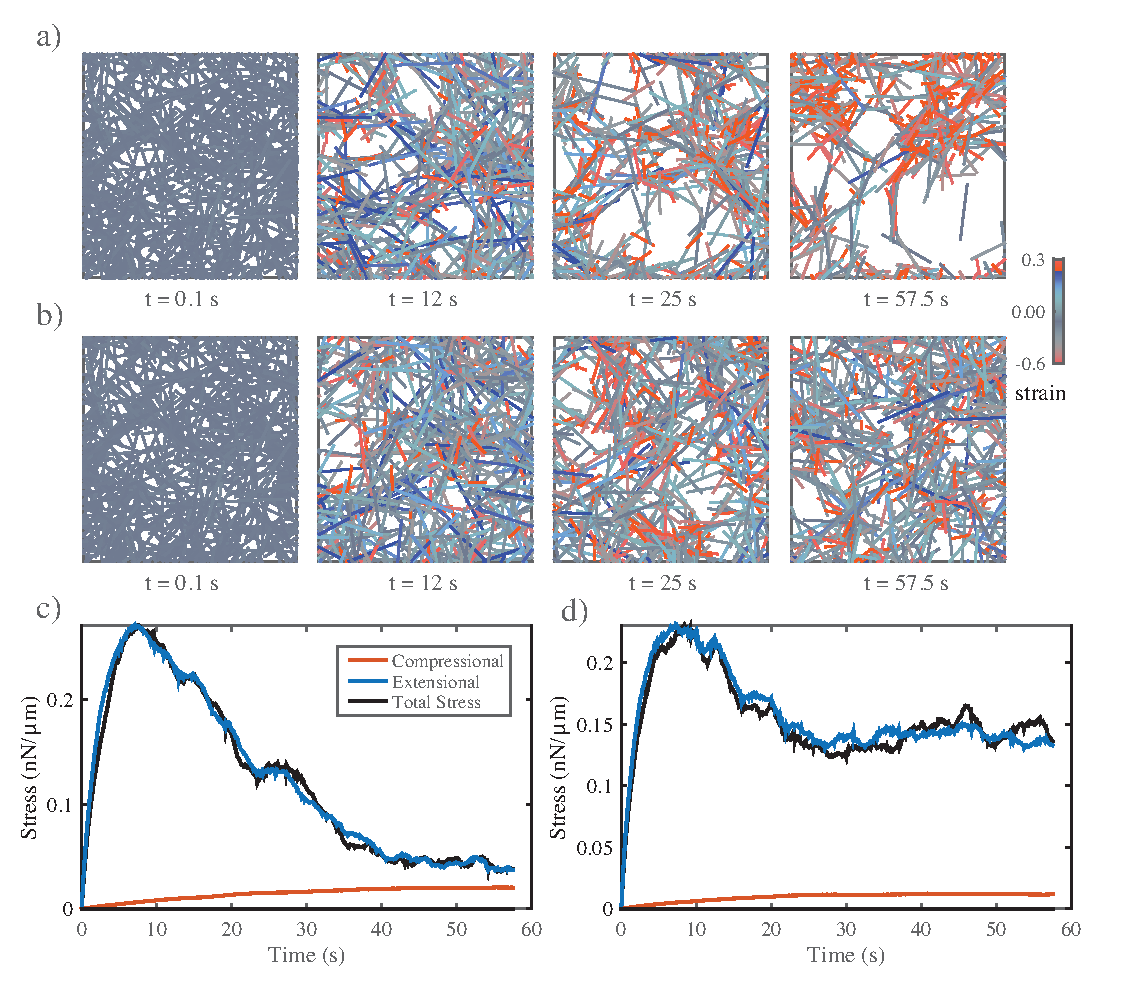
\includegraphics[width=\hsize]{figures/figureS5}
\caption{\label{fig:active_tear}  Filament turnover prevents tearing of active networks.  \textbf{a)}  An active network undergoing large scale deformations due to active filament rearrangements.  \textbf{b)}  The same network as in (a) but with a shorter filament turnover time.  \textbf{c)}  Plots of internal stress vs time for the network in (a).  \textbf{d)}  Plots of internal stress vs time for the network in (b).  }
\end{figure}

\begin{figure}[h!]
\centering
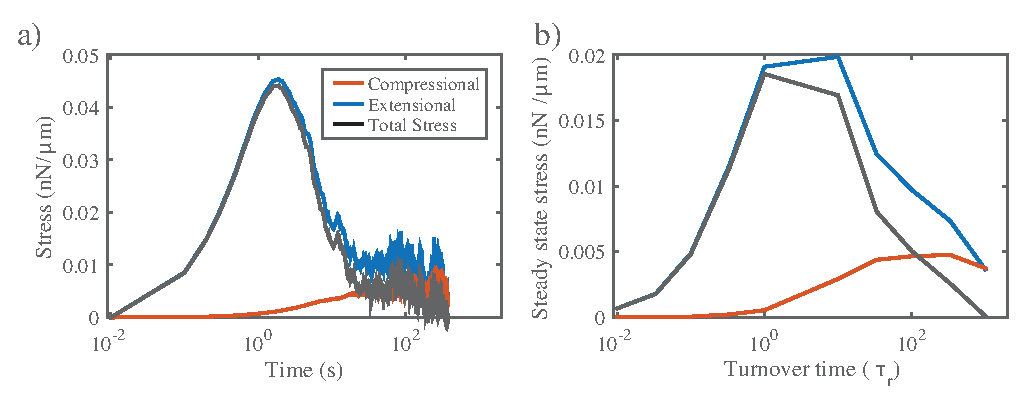
\includegraphics[width=\hsize]{figures/figureS6}
\caption{\label{fig:recycle_supp}  Bimodal dependence on turnover time matches bimodal buildup and dissipation of stress in the absence of turnover.  \textbf{a)}  Bimodal buildup of stress in a network with very slow turnover ($\tau_r = 1000s$).  \textbf{b)}  Steady state stress for networks with same parameters as in (a), but  for a range of filament turnover times.   }
\end{figure}

\begin{figure}[h!]
\centering
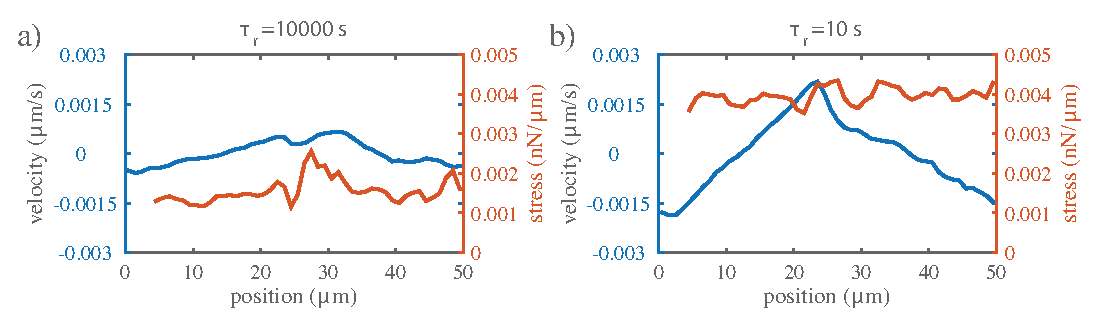
\includegraphics[width=\hsize]{figures/figureS7}
\caption{\label{fig:combo_prof}  Dynamics of steady state flow. Plots of stress and strain vs position for networks in which motor activity is limited to the right-half domain and filament turnover time is either  \textbf{a)} $\tau_r = 10000$ or  \textbf{b)} $\tau_r = 10 s$.  Blue indicates velocity while orange represents total stress, measured as described in the main text. }
\end{figure}
\end{document}


\chapter{A model of upstream actomyosin regulators in pulsed contractions}
\section{Motivation and experimental context}
\begin{figure}[h!]
	\centering
	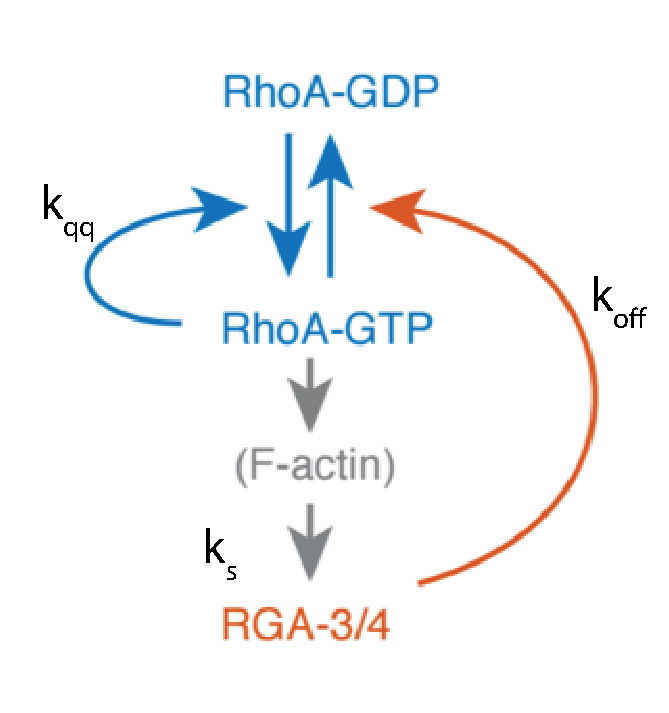
\includegraphics[width=0.5\hsize]{pulse/diagram_eq.eps}
	\caption{\label{fig:pulse_diag}  Reaction pathway with labels for coefficients associated with feedback stregths.}
\end{figure}

In many systems, cortical flows are driven not by continuous contraction of active material, but by repeated rounds of pulsatile contraction.  While it was once believed that these pulsatile behaviors could be an emergent property of actomyosin contractility itself, it is now more probably suspected that these behaviors are caused by upstream regulators of local actomyosin activity.

It is still unclear why so many systems exhibit this type of behavior, but it is nonetheless important to understand the origins of these behaviors and what differences may arise due to their presence or absence in a contractile system.  Therefore, we have begun exploring how to model both the upstream regulators that govern contractile systems as well as the downstream effects of coupling these to regulators to contractile flows themselves.

The majority of our data comes from the work of Francois Robin and Jon Michaux \cite{Robin076356}.  They have shown that upstream of both actin and myosin is a separate pulsatile biochemical circuit consisting of a combination of positive and negative feedback between a pair of proteins called Rho and RGA as depicted in Figure \ref{fig:pulse_diag}.  

To explain the dynamics I attempted to build ordinary differential equation models of local variation in active Rho and RGA concentrations.  We found that many models are effectively equivalent at producing the qualitative results.  However, this model in all of its forms is inconsistent with producing robust pulsatile behavior once the models were constrained by parameter fitting to the data. 

\section{A model for pulsatile actomyosin accumulation in \textit{C. elegans} }

I defined $\rho$ as the concentration of Rho and $r$ as the concentration of RGA, and generated association, dissociation and feedback parameters for the model. 

\begin{equation}
\label{eqn:rho_1}
	\frac{d\rho}{dt} = k_{on}^\rho \left( 1+k_{on}^{\rho\rho} \frac{\rho^n}{\rho_0^n +\rho^n} \right ) - (k_{off}^\rho + k_{off}^{\rho r} r) p
\end{equation}

\begin{equation}
\label{eqn:rga_1}
	\frac{dr}{dt} = k_{on}^{r \rho}\rho - k_{off}^r r 
\end{equation}

Next we can nondimensionalize the equation with $q=\rho/\rho_0$, $s=k_{off}^{\rho r}/k_{off}^r r$, and $\tau=k_{off}^r t$, and rename parameters for simplicity.

\begin{equation}
	\frac{dq}{d\tau} = k_q \left( 1+k_{qq} \frac{q^n}{1 +q^n} \right ) - (k_{off} + s) q
\end{equation}

\begin{equation}
	\frac{ds}{d\tau} = k_s q - s
\end{equation}




\subsection{Analyzing parameter space of the model}


Just from analyzing the null-clines of this model we can gather a lot of information about the qualitative behavior of this model.  

\begin{equation}
	s_q =\frac{k_q}{q} \left( 1+k_{qq} \frac{q^n}{1 +q^n} \right ) - k_{off} 
\end{equation}

\begin{equation}
	s_s = k_s q
\end{equation}

\begin{figure}[h!]
	\centering
	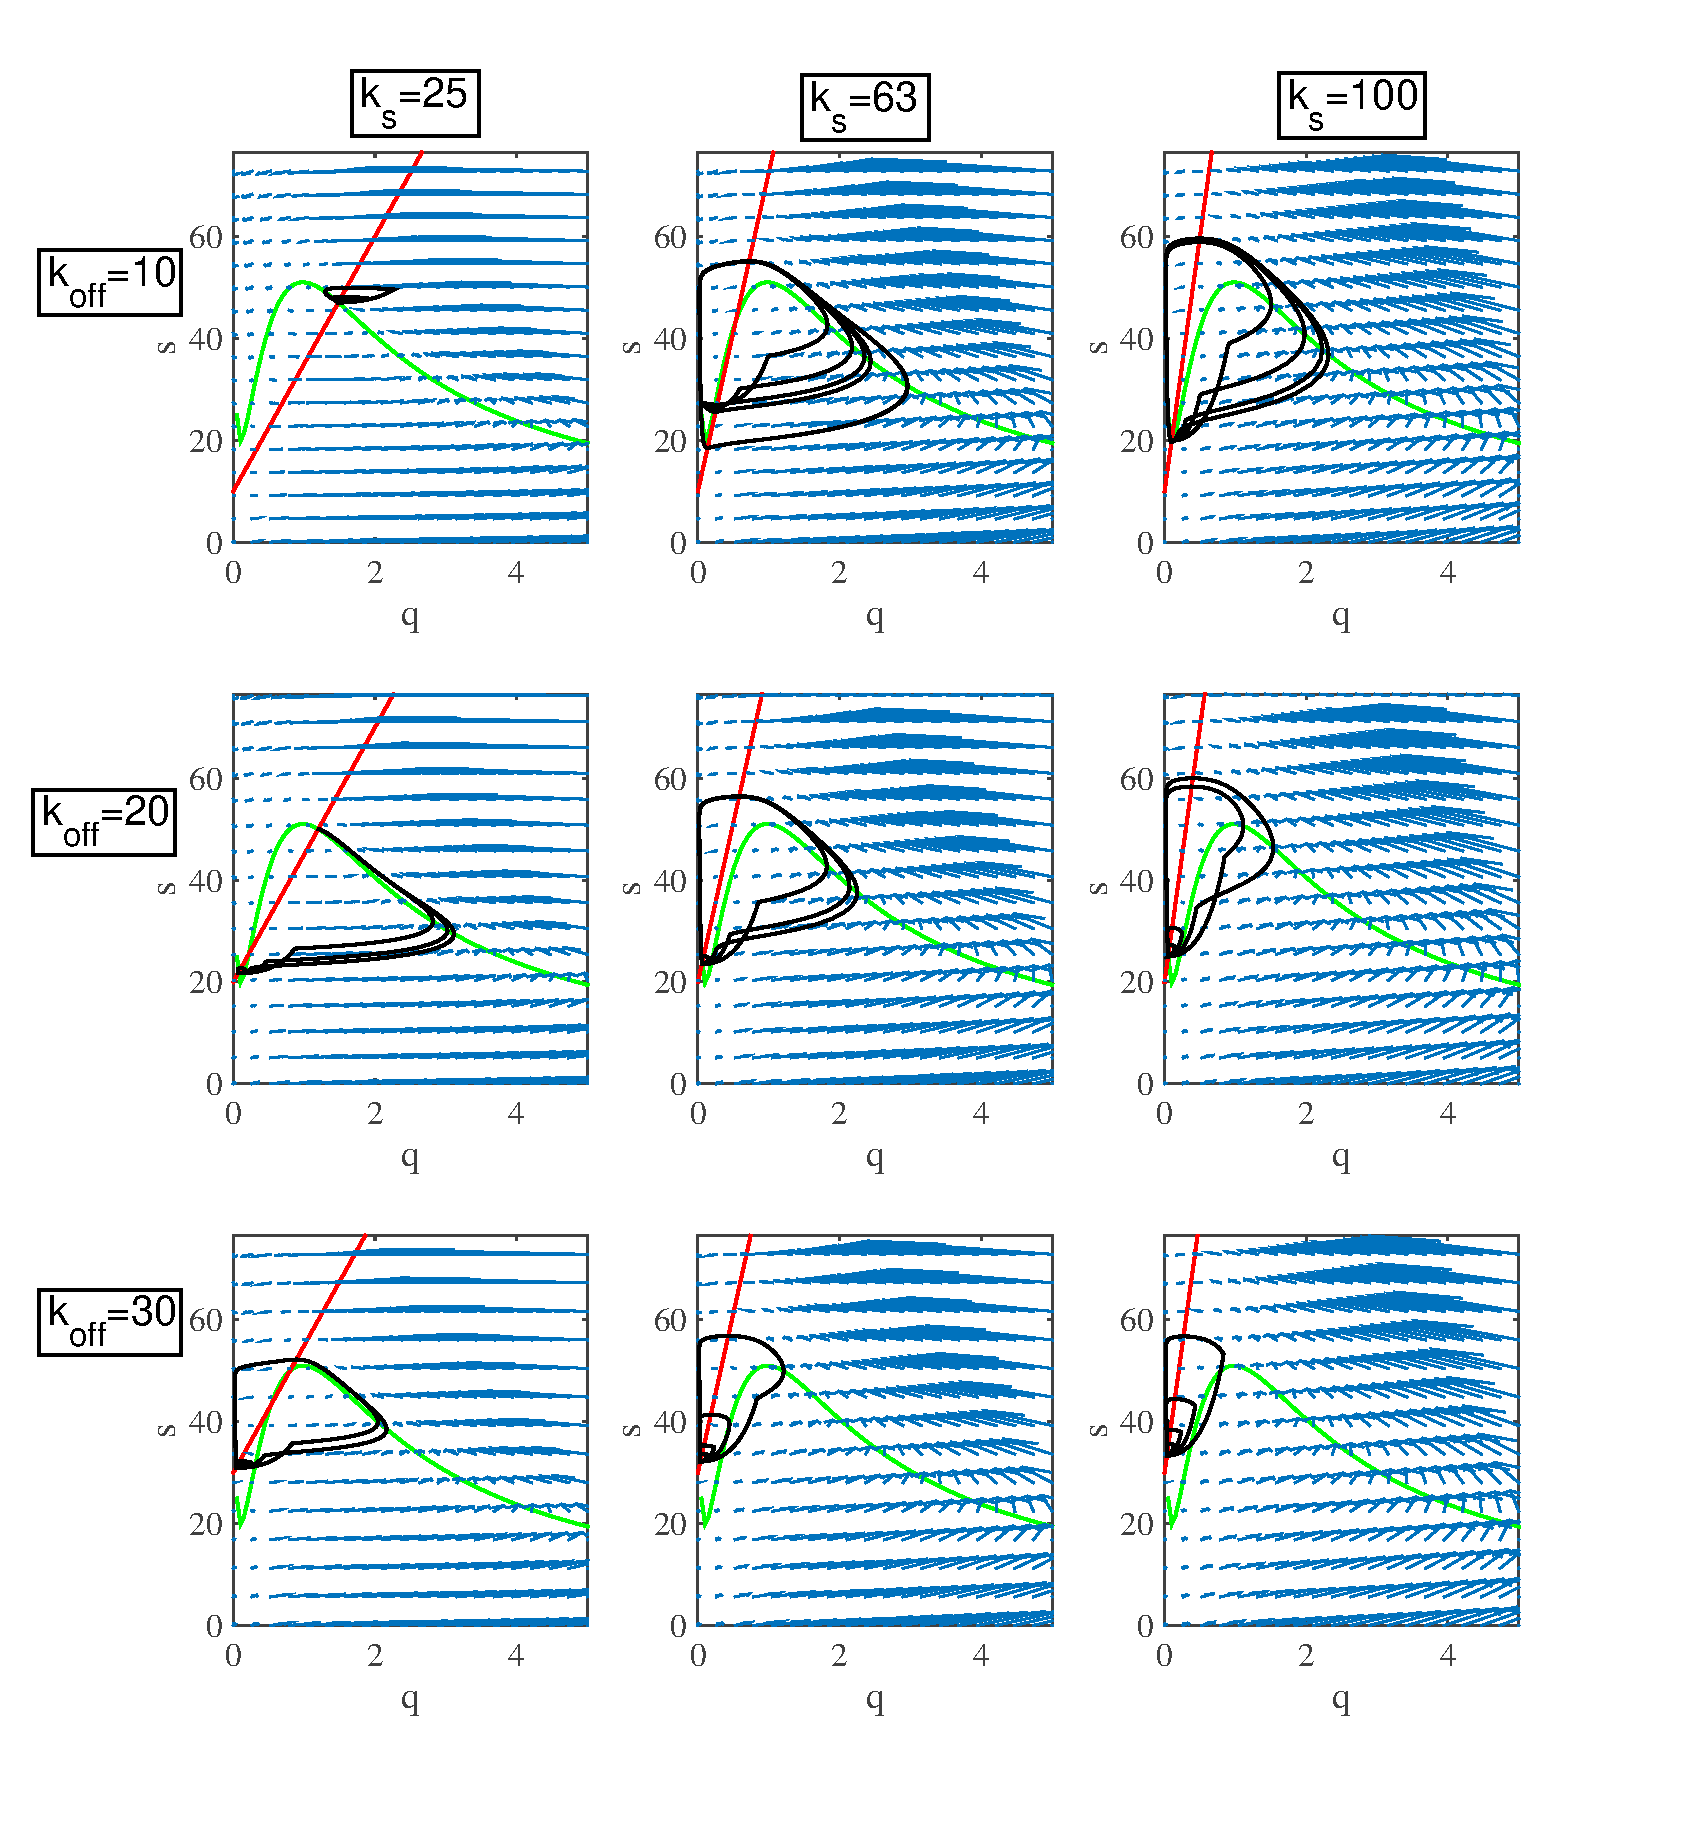
\includegraphics[width=\hsize]{pulse/phase_tester.eps}
	\caption{\label{fig:pulse_test}  Perturbation simulation results plotted on phase planes for a variety of parameters.  }
\end{figure}

The $s_q$ null-cline appears as an inverse relation between $s$ and $q$, with a hump around $q=1$ whose height is dictated by the strength of the $q$ positive feedback, $k_{qq}$.  The $s_s$ null-cline is simply a straight line whose slope is governed by $k_s$.  The dynamical system is only able to attain pulsatile behavior when the $s_s$ null-cline runs parallel and to the left of the hump in the $s_q$ null-cline.  This gives two effective conditions on pulsatility: 1) If $k_{qq}$ isn't much larger than 1, there will not be any hump, and so there cannot be any pulsatility. 2) If $k_s$ and $k_off$

To test this prediction, I implemented an automated search of the model's parameter space.  The test worked by adding perturbations of fixed strength to the equilibrium state, and observing whether the response of the system exceeded the perturbation. As shown in Figure \ref{fig:pulse_test} for a number of simulation parameters, the response function could vary from having just a stable fixed point ( $k_{off}=10$ and $k_s=25$) to having stable oscillations ( $k_{off}=10$ and $k_s=63$) to having pulses ( $k_{off}=20$ and $k_s=63$).  Figure \ref{fig:pulse_test} also shows the null-clines for each case, which can be used to interpret whether pulsation is possible.

\begin{figure}[h!]
	\centering
	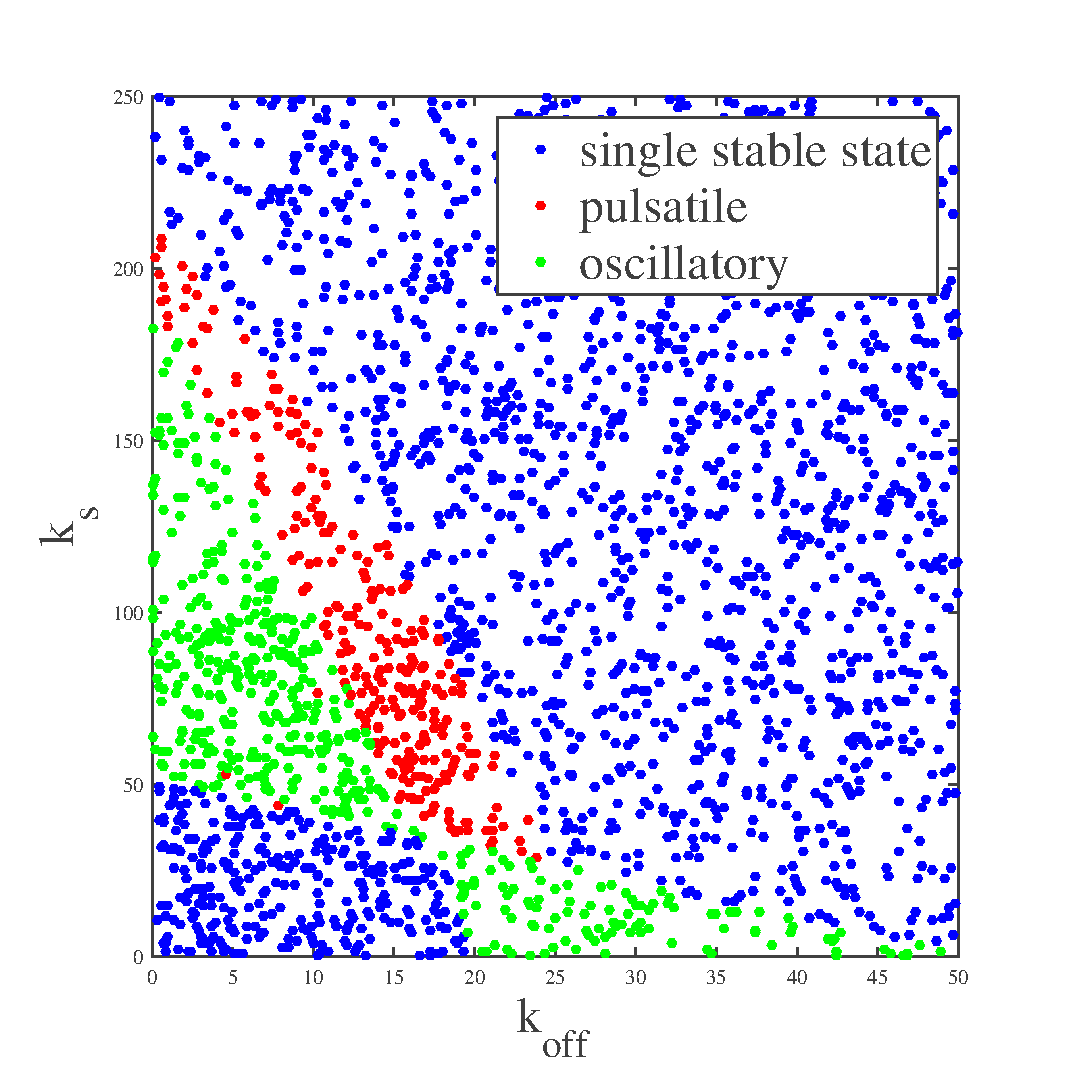
\includegraphics[width=\hsize]{pulse/k_phase.eps}
	\caption{\label{fig:pulse_k_phase}  Phase diagram of for $k_q=1$ and $k_qq=100$.}
\end{figure}

Using this automated system, I was able to generate 1600 simulations and classify them automatically based on the ratio of the magnitude of the perturbation to maximum response (to determine if positive feedback drove excitation) and whether the maximum was attained multiple times (to differentiate pulses and stable oscillations).  This resulted in a phase diagram of the behavior as shown in Figure \ref{fig:pulse_k_phase}, with the three colors indicating the behavior of dynamical systems in that regime.  The size and shape of the pulsing region of phase space was a direct result of the strength of positive feedback ($k_{qq}$)  with stronger feedback allowing more of phase space to permit pulsing and oscillations.

\begin{figure}[h!]
	\centering
	\includegraphics[width=\hsize]{pulse/randomized_simulation.eps}
	\caption{\label{fig:pulse_rando}  }
\end{figure}

Finally, using this understanding of the phases behavior of the system, I implemented a stochastic dynamical equation to test the response to noise.  As indicated in Figure \ref{fig:pulse_rando}, a basal level of noise was able to trigger robust pulses in both Rho and RGA for certain parameters. Taken together this analysis indicated that our biochemical reaction circuit for Rho and RGA feedback could in principle account for the excitable dynamics exhibited in the system.

\section{Simplified model and data fitting}
\subsection{Fitting techniques}
\begin{figure}[h!]
	\centering
	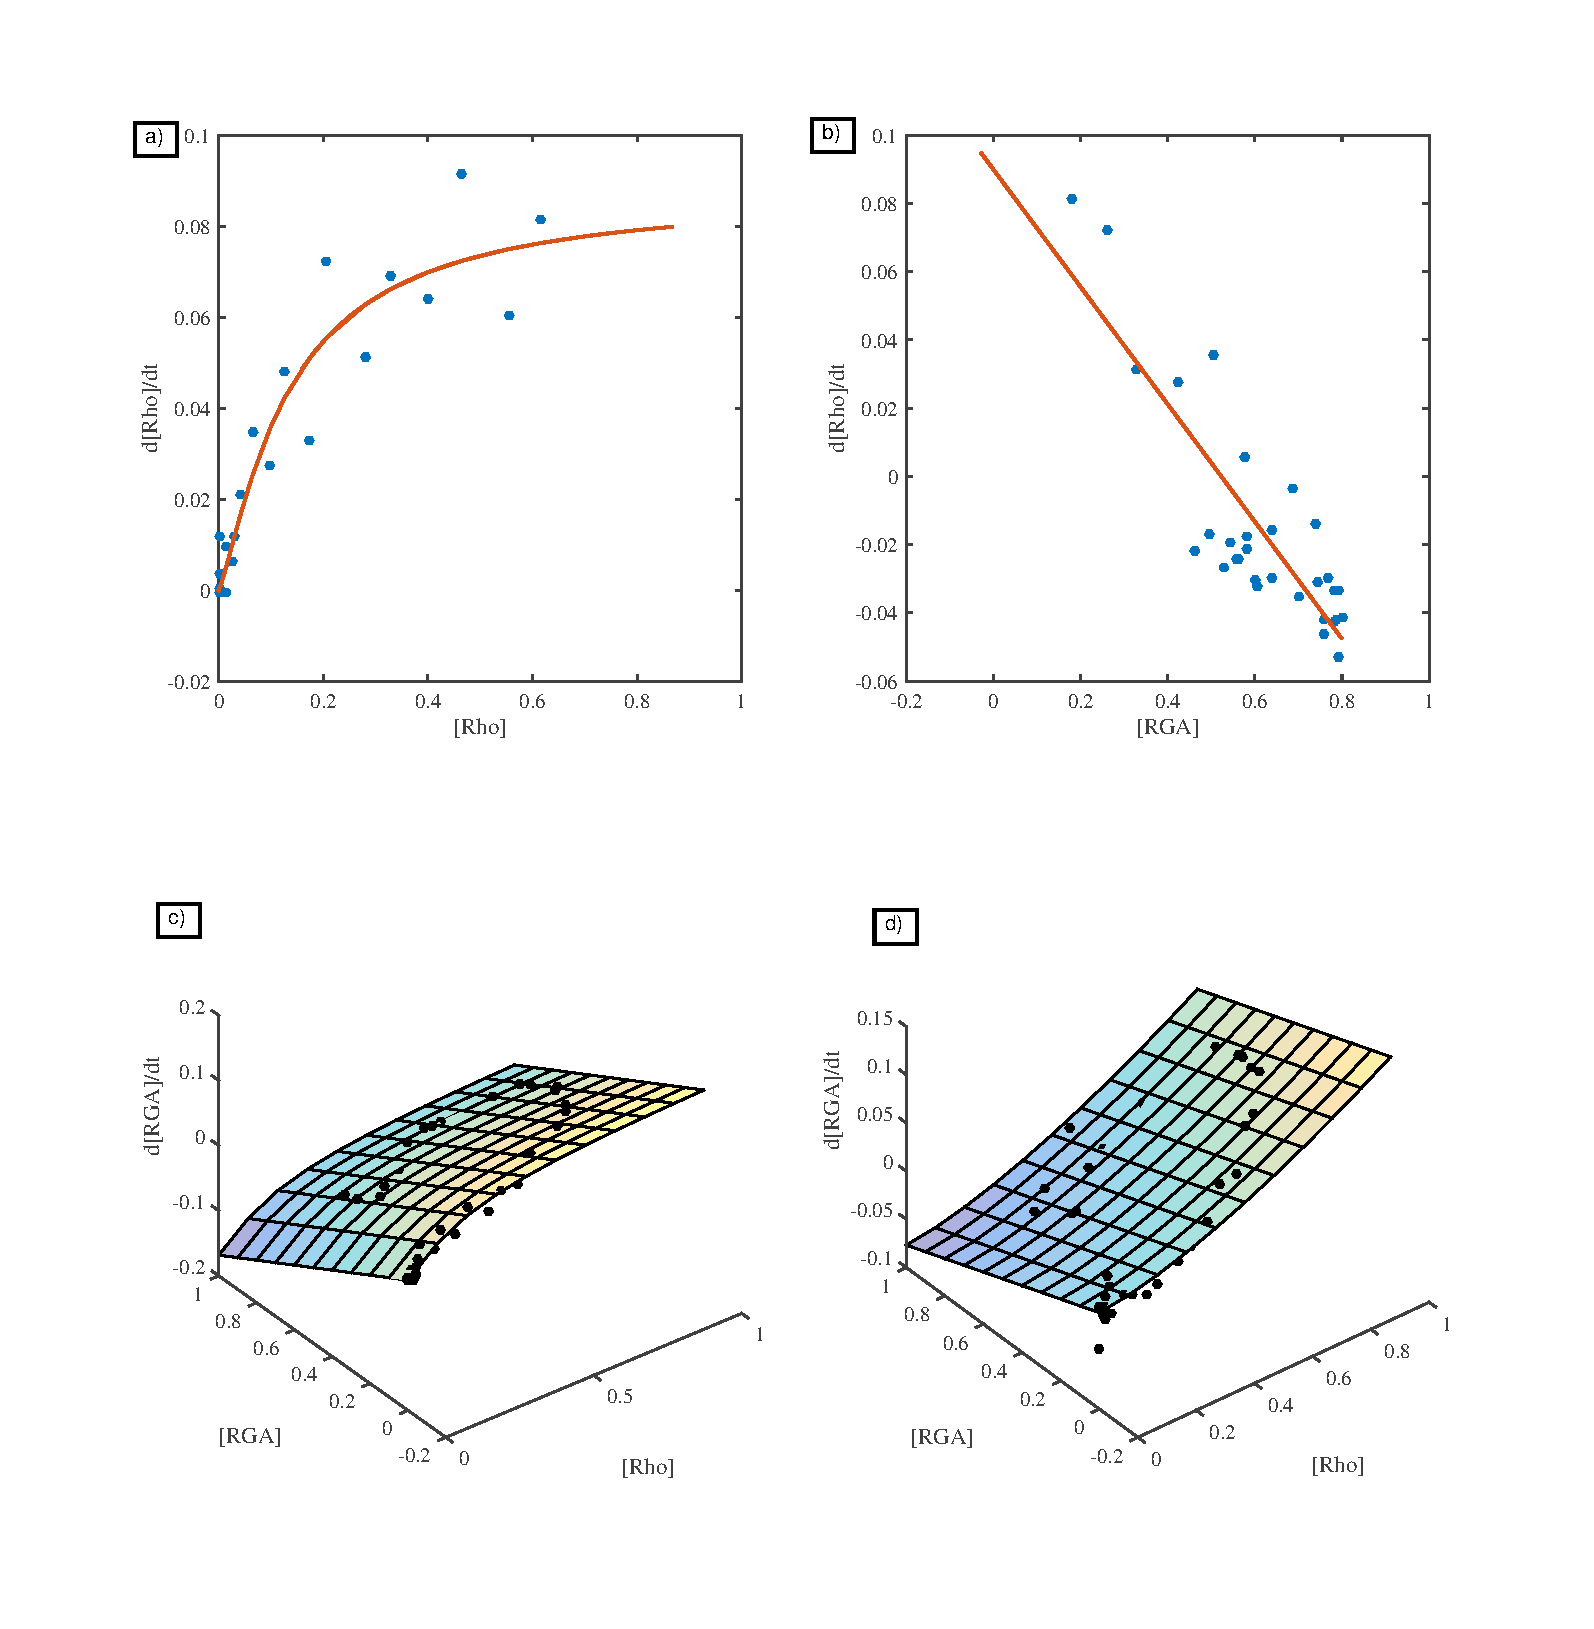
\includegraphics[width=\hsize]{pulse/fitting_plot.eps}
	\caption{\label{fig:pulse_fit}  Multiple methods of fitting.}
\end{figure}

Although this model accounted for the qualitative behavior, we wished to determine whether it could be corroborated by fitting to the data presented in the paper. To experiment with fitting the normalized data, I created a reduced model, where the equilibrium concentration had been renormalized to 0 for both Rho and RGA, and the feedbacks between Rho and RGA are allowed to be non-linear.  

\begin{equation}
	\frac{dq}{d\tau} =\alpha \frac{q^n}{1 +q^n} - s q^k
\end{equation}

\begin{equation}
	\frac{ds}{d\tau} = \beta q^{(m-k)} - s
\end{equation}

These equations resulted in a family of models with different levels of feedback, depending on the values of $n$, $m$, and $k$.  I fit models with a variety of exponents and found that any model with $k\approx0$, $n>1$, and $m\approx2$ gave the best overall agreement with the greatest robustness.  
\begin{figure}[h!]
	\centering
	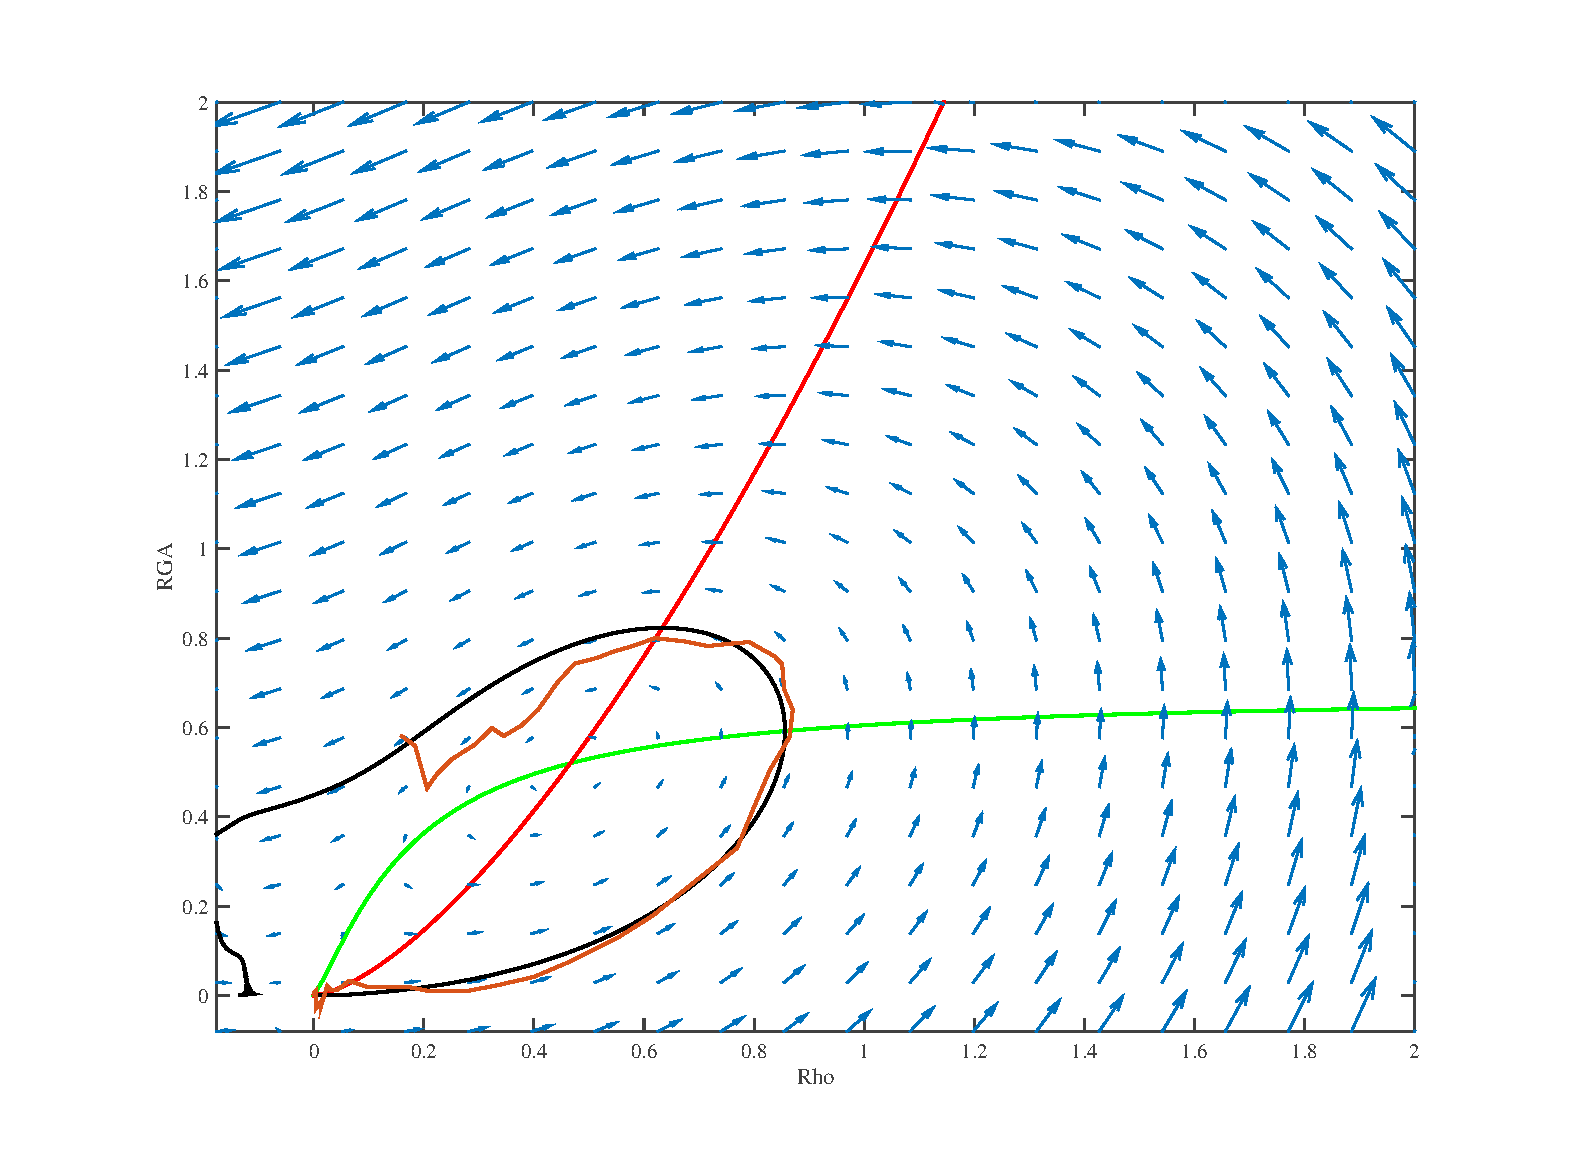
\includegraphics[width=0.45\hsize]{pulse/simple_model_fit_phase.eps}
	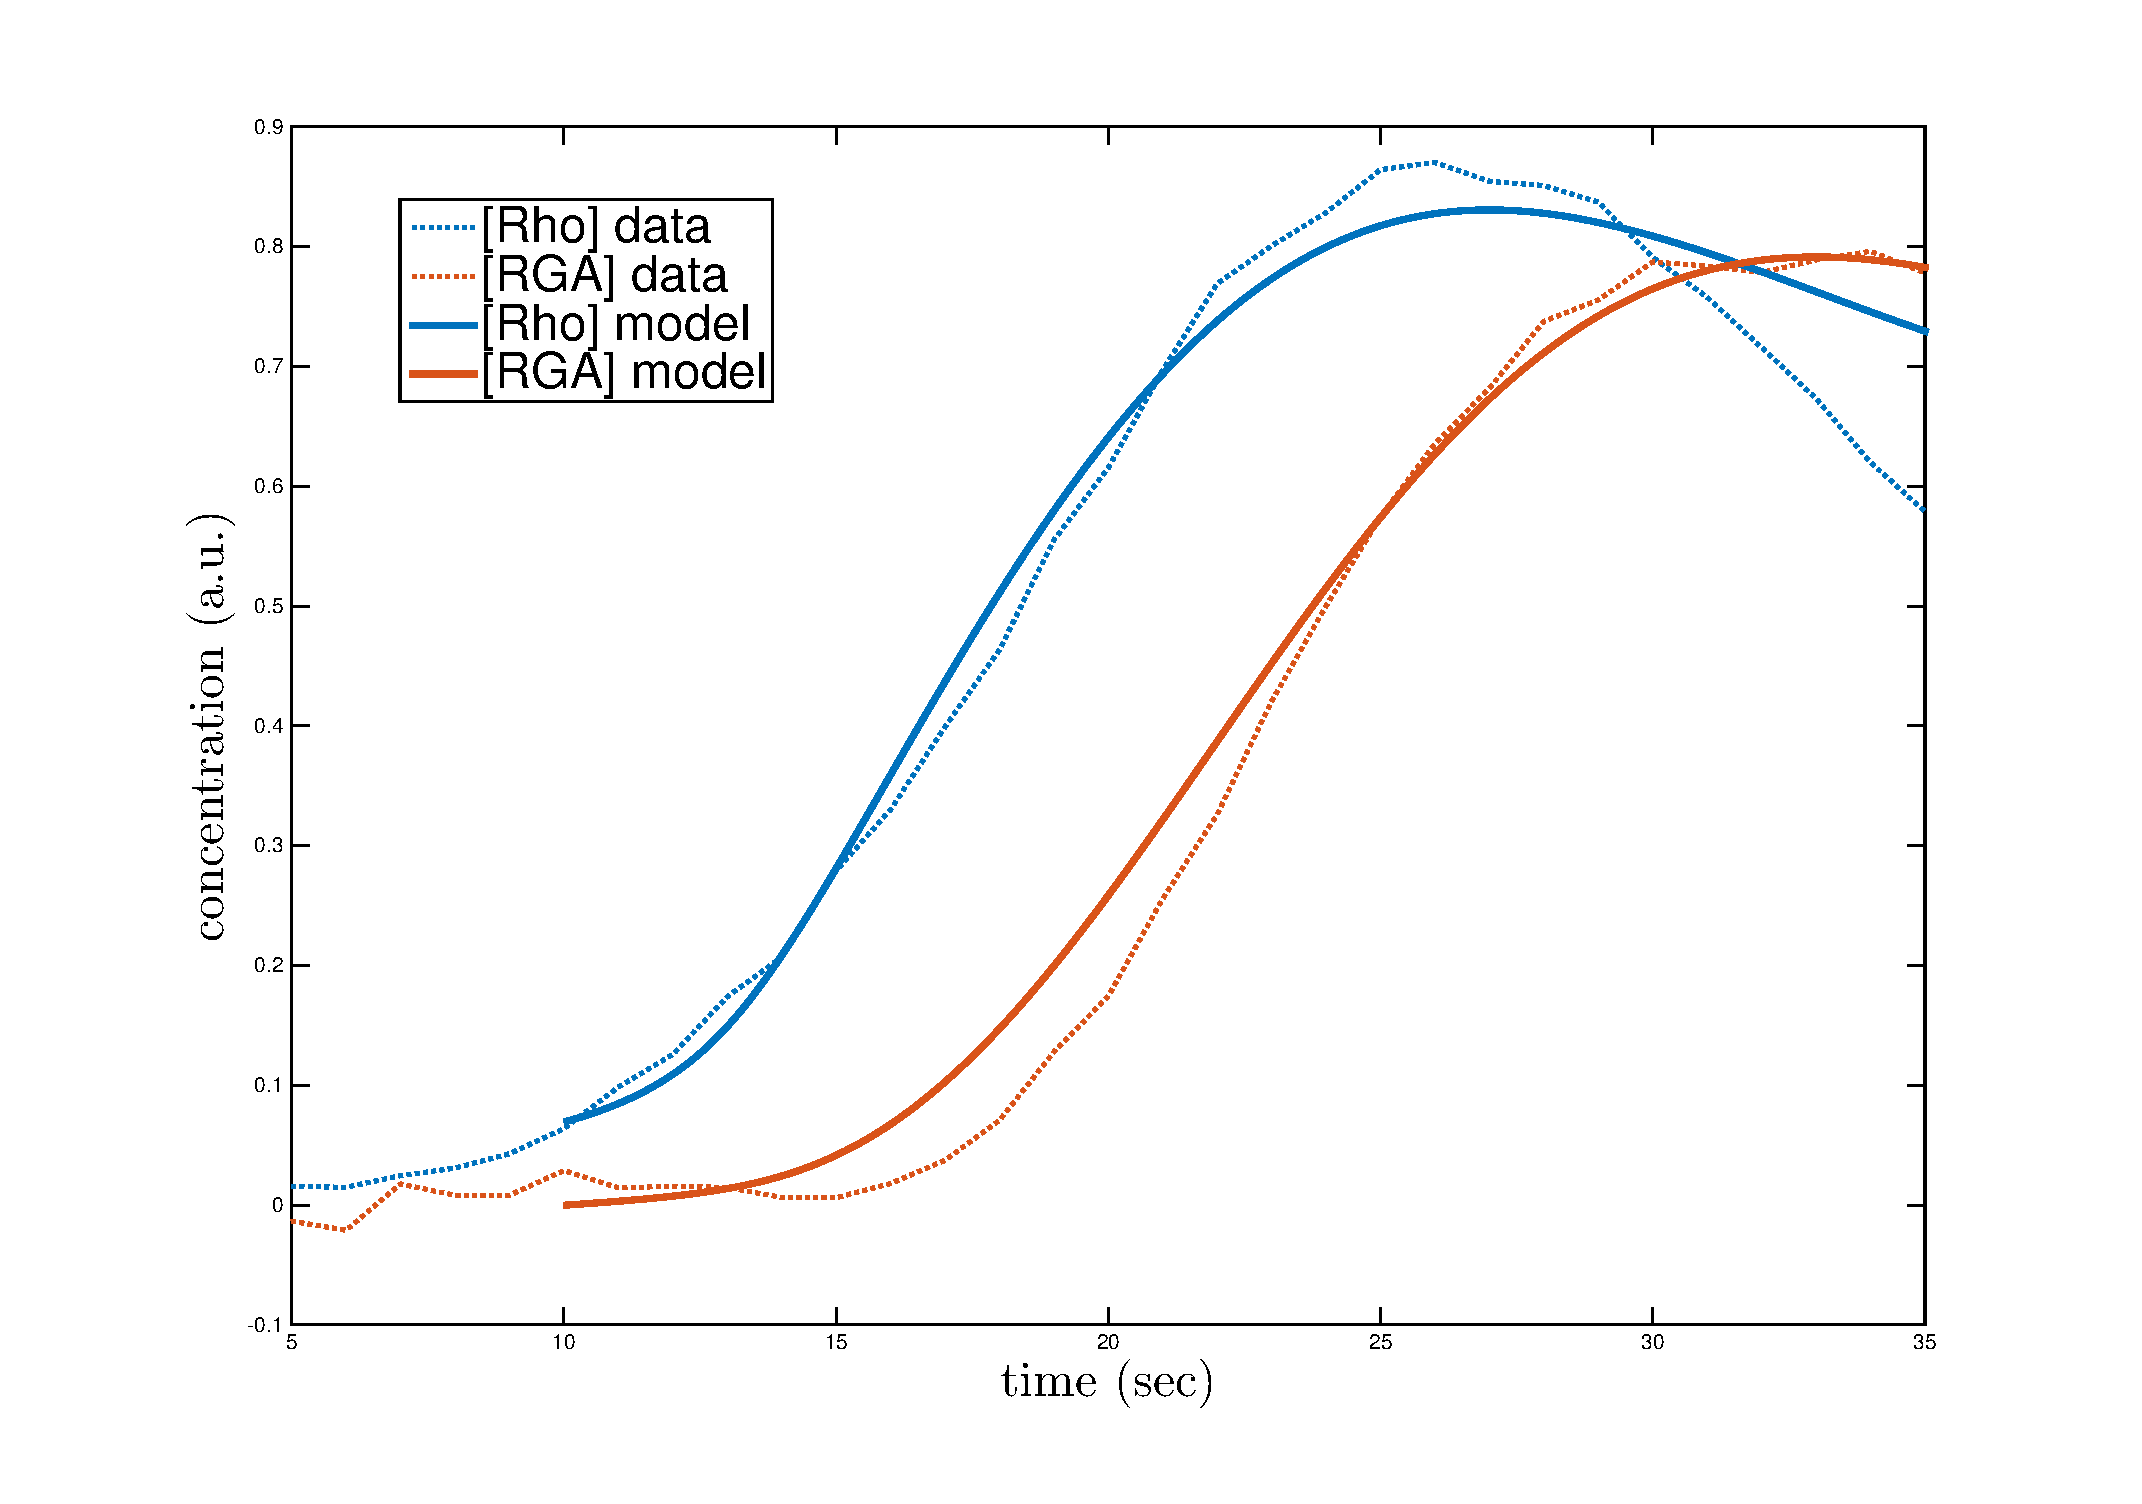
\includegraphics[width=0.45\hsize]{pulse/model_profile.eps}
	\caption{\label{fig:pulse_fit_sim}  Simulation results and fitted data for model with $m=2$ and $k=0$. Displaying simulation results and the data used to fit the simulation on a phase plane (left) and as pairs of time plots (right).}
\end{figure}
I used two different methods to fit the Rho and RGA data to determine the most appropriate model parameters.  The first required subsecting the data to fit only datapoints where some terms in the equation were presumably close to constant (Figure \ref{fig:pulse_fit}a,b).  For example, as long as RGA concentration remained relatively small, the equation for Rho could be taken to consist of only the Rho self-feedback function.  The second method allowed fitting all of the data the equations at once (Figure \ref{fig:pulse_fit}c,d).  The second method is clearly more accurate, but it comes at the cost of being slightly more difficult to explain to the lay-biologist.

\begin{figure}[h!]
	\centering
	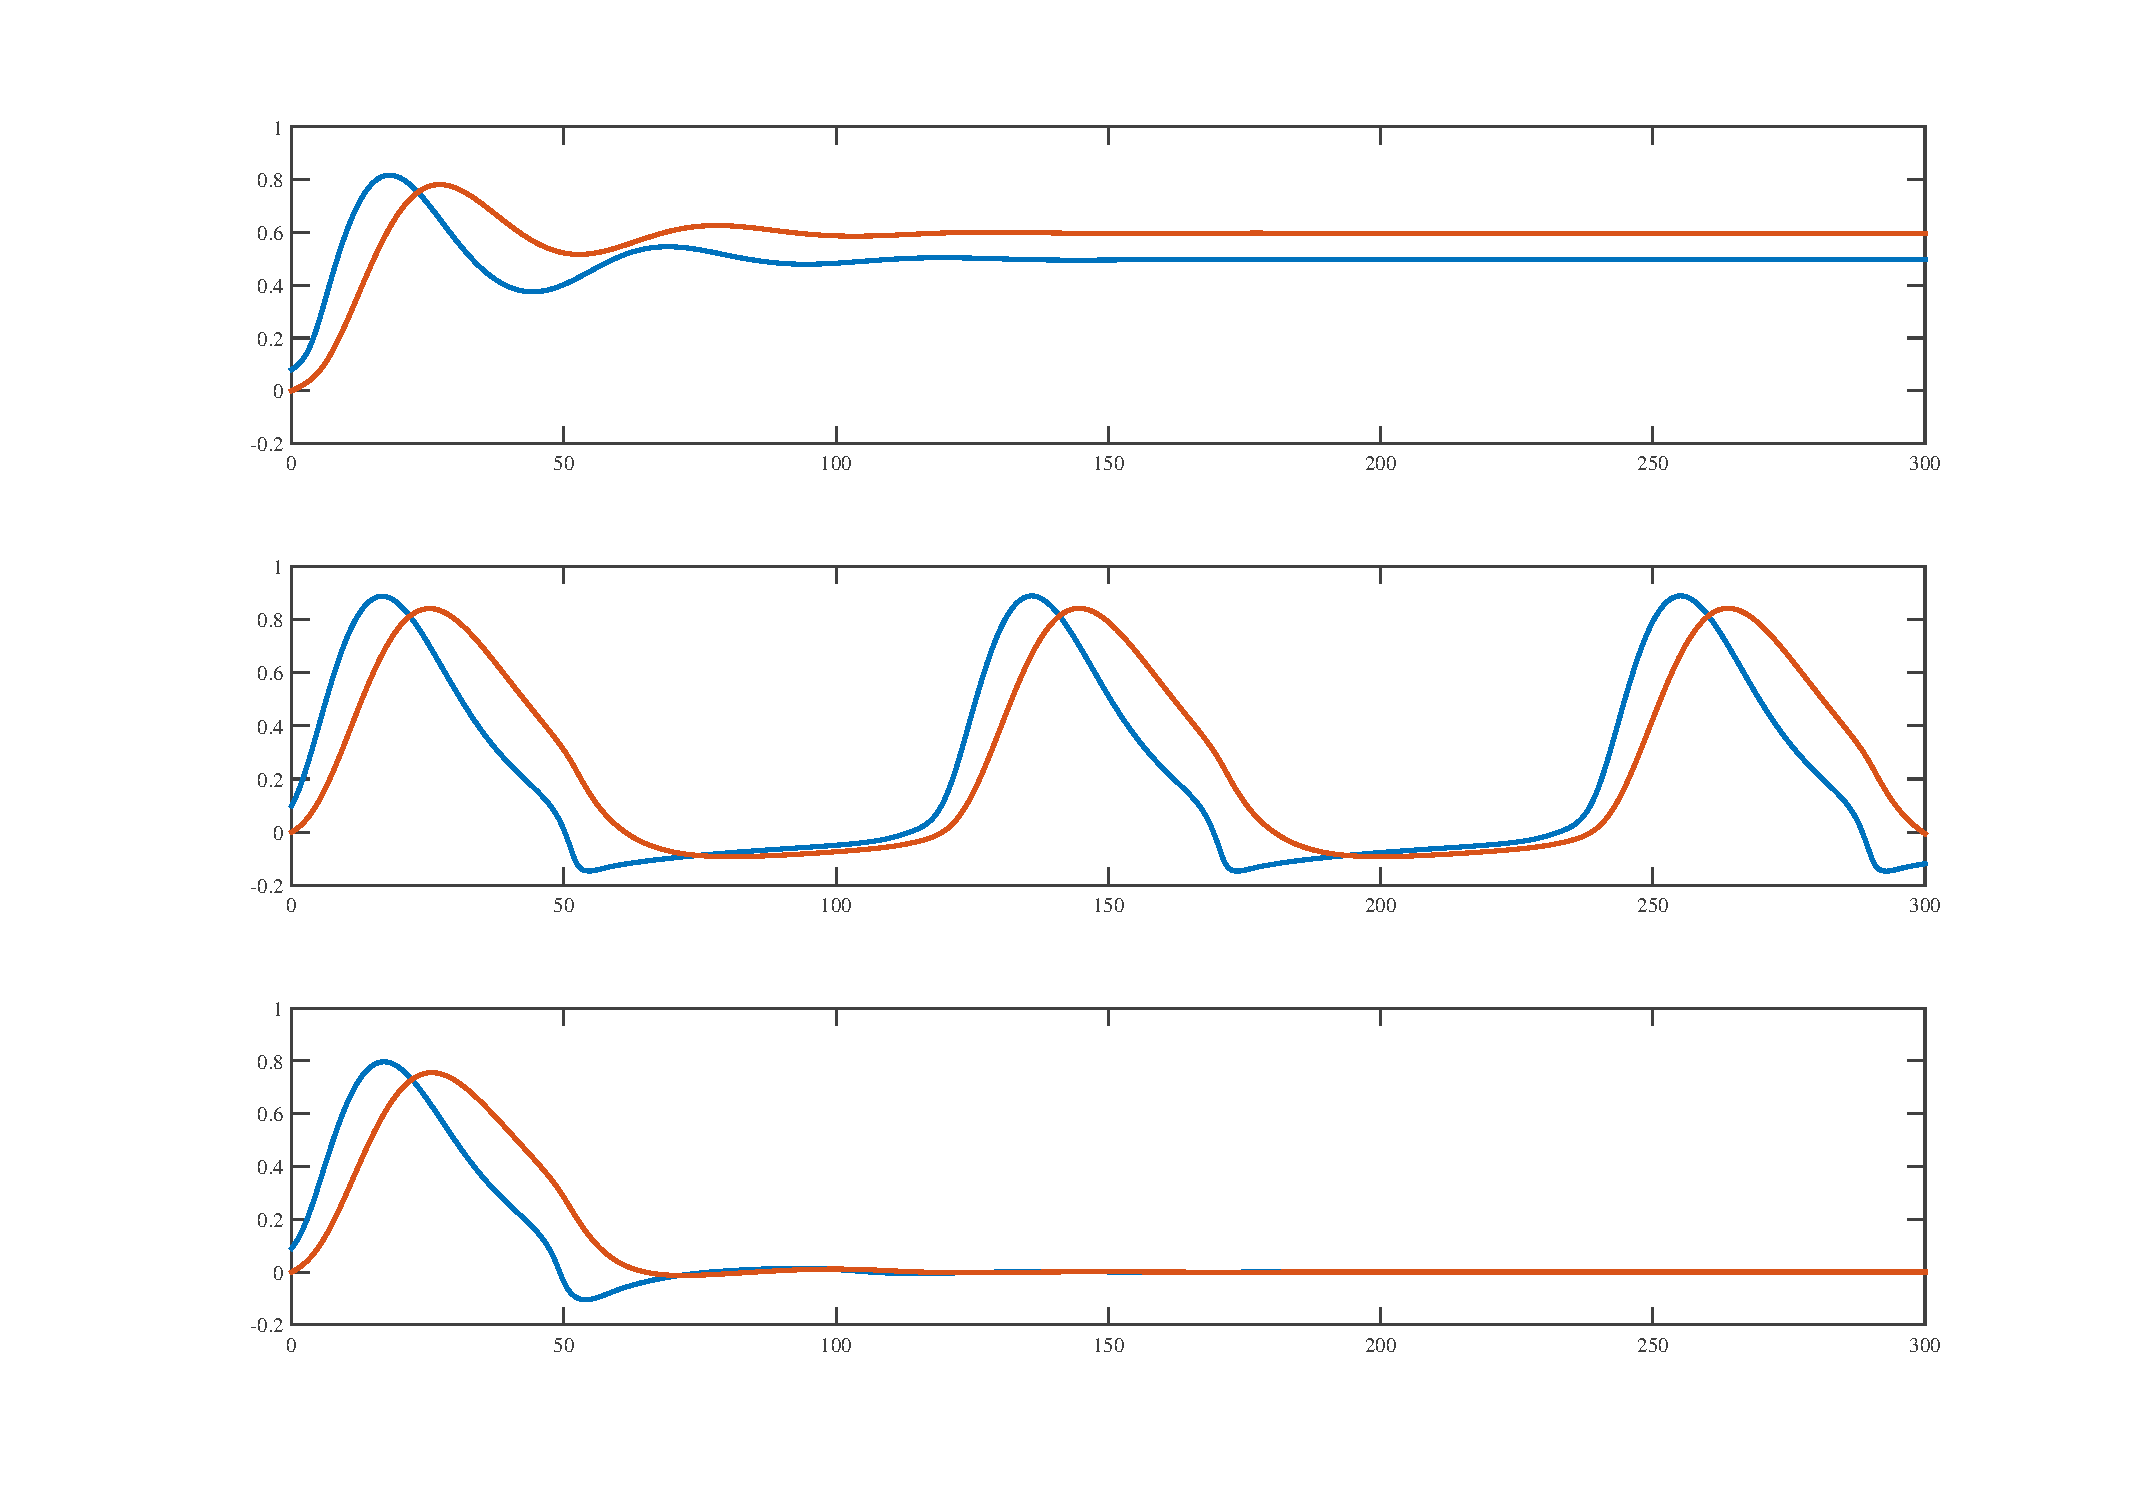
\includegraphics[width=\hsize]{pulse/model_compare.eps}
	\caption{\label{fig:pulse_fit_compare}  Small variation in simulation parameters can have large qualitative effects.}
\end{figure}

The resulting fitted models could then be used to run simulations.  As shown in Figure \ref{fig:pulse_fit_sim}, the models and fitted data were largely indistinguishable relative to the error in the data.  Although the model was quite successful at recapitulating the original data, I found that the resulting models were not necessarily.  For example by changing the value of the parameter $\alpha$ by 25\% and rerunning the fits, I could tune the system from a stable system to pulsatility and into an oscillatory regime (Figure \ref{fig:pulse_fit_compare} ).  Therefore, it appears that this model is not incredibly robust to minor variations in parameters. 


\section{Conclusion}
\begin{figure}[h!]
\centering
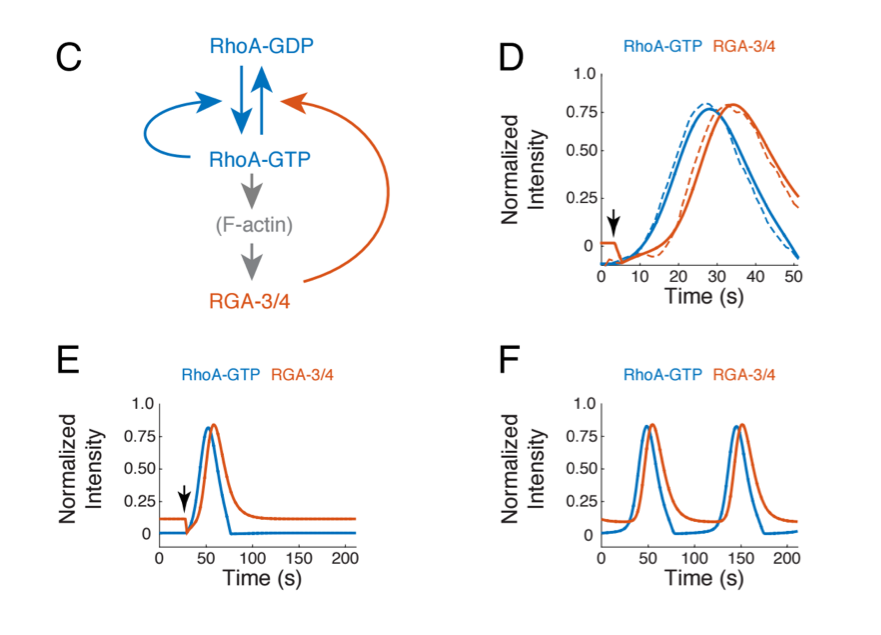
\includegraphics[width=\hsize]{pulse/final_fig.png}
\caption{\label{fig:pulse_final}  Final figure as it appears in Reference \cite{Robin076356}.}
\end{figure}
Ultimately, a model similar to \ref{eqn:rho_1} and \ref{eqn:rga_1} was utilized in the final paper in combination with at the 2D fitting routine outlined in Figure \ref{fig:pulse_fit}c,d.   In short, all models performed fairly well at describing the qualitative features of the data, but none were very effective at generating a quantitative match with great robustness.    We believe this is indicative of the need to perhaps extend to incorporating spatial effects in driving the dynamics of active material pulses.  Based on the theoretical results of \cite{PhysRevLett.106.028103}, we attempted to incorporate our upstream regulatory model into a 1D active fluid.  This ongoing work will hopefully tie together the spatial and temporal interdependencies driving this system into its interesting non-equilibrium state.



\chapter{Future Directions}

\section{Conclusion}
In this work I have presented my attempts to measure and model the dynamics of cortical flow. I have done this by assisting in developing a technique to improve our ability to measure actin dynamics in the cell cortex, and by developing mechanistic models of actomyosin and its upstream regulators. Although this work was able to establish several useful findings, there were shortcomings in the methodology used and the assumptions implicit in the modeling framework.  In the next section, I outline shortcomings in my modeling methodology and potential ways to resolve those shortcomings in the near term. I discuss some of the limitations and broader implications of the model presented in Chapter 3. Next, there have been some very recent publications that have undertaken to explore the same subject area that I have described in this thesis, namely actomyosin dynamics with turnover.  In Section \ref{sec:compar_lit}, I compare my work to two of the most pertinent studies, and draw conclusions about the generality or specificity of findings in each work.  Finally, I end this chapter with a description of a simple set of experiments that I believe will be beneficial in validating the theoretical conclusions of my modeling efforts.



\section{Limitations of the present modeling approach and how these could be addressed in future work}

\subsection{Pure friction for cross-link interaction}
A key feature of my model in comparison to others is that the mechanism of cross-linking is a frictional coupling between filaments.  The motivation for this (as discussed above) is to provide a mechanism of coupling filaments on short timescales while allowing the rearrangement of filaments on long-timescales.  Frictional coupling serves as a simplification of the processes of cross-linking binding, deformation under force, and unbinding, and has been used previously \cite{theo_friction,theo_frictionSam,theo_molefric,mol_fric,theo_hydroish2,theo_frictionShila} to effectively simplify the aggregated action of many molecular binding and unbinding events. In Appendix \ref{chap:slippage}, I give a detailed account of how one could derive such a frictional coupling from the averaging of many reversible elastic attachments.  

Nevertheless, the assumptions used in generating this frictional coupling are a generalization and it is possible that specific details governing the cross-linking in cells could impact the physics in ways that my model cannot account for.   For example, my particular implementation of frictional coupling necessitates that the coupling is linear in the velocity, but theoretically any force-velocity relationship could exist between the two cross-linked filaments.  By modifying the equations of motion, I could theoretically incorporate non-linearities in the force-velocity curve, allowing, for example, a frictional coupling that was dependent on the square or the cube of the velocities.  However, it seems that this would only have an impact on the quantitative relationships between, say, applied stress and network strain rate, giving rise to non-Newtonian viscosities.  While this would make the analysis much more complicated due to the inability to scale out things like applied stress, it wouldn't have much of an impact on the qualitative shape of the results I've drawn.

A more serious concern is the possibility that even on very long timescales, the filaments do not experience purely viscous coupling at all, but that some amount of elastic constraint exists indefinitely.  This could arise from effectively irreversible cross-link binding, or from another active process which serves to prevent filament rearrangement after they reach a stable deformed configuration (e.g. alignment of bundles could stabilize particular deformed geometries).  The present implementation of my model does not allow for any irreversible attachments of cross-linkers.  However, in a certain sense, my model is able to mimic irreversible cross-linking by allowing the frictional coupling to be arbitrarily high.  It might be interesting to explore how networks respond to a subset of filaments undergoing cross-link rearrangement on disparate timescales in future work. This might have several interesting effects.  It would probably affect the timescale of transition to viscous flow in passive networks and impede local rearrangements that lead to dissipation of contractile stress on short timescales.  These two effects would complicate the dependence of steady state stress and effective viscosity on network parameters on longer timescales, impacting the conclusions I've drawn about the rates of flow.  


\subsection{Linearization of filament compliance and myosin force-velocity}
Another simplification assumed in my model is the piecewise linearization of the filament force extension curve and the myosin force-velocity curve. In both cases my model can easily be extended to incorporate more subtle details of the relationship, similar to the case for linear friction, but I believe that this extension will only make the model increasingly complex without changing the qualitative outcomes, as I will explain below.

First, the linear approximation of the myosin force-velocity curve is unlikely to alter the main predictions of the model for the same reason as linearization of the cross-link friction force-velocity curve.  The actual relationship between stall force and velocity resembles an inverse relationship rather than a negatively sloping linear relationship as I approximate it in the model \cite{howard2001mechanics}.  Thus, as the real  motor transitions from freely moving to stalled it will not transition linearly, but will initially build force slowly and then more rapidly as it reaches stall.  This will have some very subtle impacts on the time progression of force buildup, but it is unlikely that there would be any major effects that could prevent force buildup or stall altogether.  Thus the time series of force buildup could be different, but the qualitative effect would be the same.

The piecewise linearization of the force extension curve as a worm-like chain is a bit more complicated.  The simple linearization makes it incredibly simple to model a general semi-flexible filament-like structure, which can include an actin, a microtubule, a bundle of actin filaments, or a carbon nanotube, in a manner that is agnostic to the specific non-linear relationship that arises due to the local mechanics and geometry.  However, in order to generalize the asymmetry between contraction and extension, one still has to select a threshold to define the two windows of strain.  In my model, I used an arbitrary distinction between extension and compression around the relaxed length, but this is an oversimplification.  In reality, the non-linearity could arise at some offset extension (if one were  interested in slack being pulled out of the filament) or compression (if one were interested in buckling).  Needless to say, this offset could easily be added to the piecewise linearization process without complicating the analysis much further.  Additionally, this linearization is very useful to gain analytcal insight as it allows the asymmetry factor to fall out of the any measurements regardless of the specific deformation regime that is being probed in a given simulation.  In contrast, if one were to look at a wormlike chain model instead, they would find that for some deformations there would be no asymmetry, then for slightly more deformation there would be a factor of, say, 10 asymmetry and then for even more deformation you would reach an infinite difference between extension and contraction.  Thus, you must draw all of your conclusions relative to the specific window of deformation, and some of the general structure of the mechanical picture can be lost.  In contrast, the linearization means that for any deformation the difference in the force applied between extension and compression will be a constant.  While this is advantageous for making the analysis very clear, it has the drawback of making the network's rigidity linear when it would actually show many more interesting non-linear properties.  However, if one were interested in making quantitative predictions for a very particular and well-characterized kind of filament network, a more detailed force-extension curve could easily be implemented in this framework.

\subsection{Absence of Thermal fluctuations}
In my model, I do not incorporate any thermal fluctuations into the motion of filaments or motors.  For individual filaments in solution, thermal fluctuations can give rise to large filament deformations and long-range diffusion \cite{PhysRevE.69.061921}.  However, it is unclear how important these motions are on the timescales of interest when cross-linking connects the network into a macroscopic structure.  Single molecule measurements  in \textit{C. Elegans} embryos \cite{Robin:2014aa} suggest actin filaments are subdiffusive ($\langle r^2 \rangle = Dt^{0.6}$) with very low short term diffusivity ($D = 0.057 \mu m^2 /s$).  In contrast, the advective flows found in embryos and motile cells move material at upwards of ten microns per minute \cite{Munro2004413, amoeba1, amoeba3}.  This results in a Peclet number between 3 and 6, and allows us to assume that for flowing cortices, advective motion of the connected network dominates.

Because the goal of this work is to derive general properties of how flows of any speed arise, I also want to point out that this non-thermal description can be coupled with an understanding that diffusive motion can sometimes dominate.  Since we can always demark a difference in flow speeds between those networks where the macroscopic motion dominates versus those where diffusive effects dominate, one can ignore thermal effects provided we remember that at low enough advection speeds diffusion will again dominate. I assume that any time I observe very little motion in my simulations, a real system will be in an effectively diffusive state and we can use our understanding of passive networks to describe the thermal motions of the filaments.  Thus, when my simulations result in very small flow rates, I assume that these flows will fail to outpace diffusion and, therefore, will be effectively nullified.  However, in the future, it may be worthwhile to explicitly incorporate these effects in order to directly observe the transition between diffusive and advective motion.

\section{Probing more complex mechanisms of turnover}

Another notable simplification in this work is the method of incorporating filament turnover. The mechanism I employed causes entire filaments to be reset at random, which may not accurately reflect  the mechanisms by which filaments are depolymerized and repolymerized in living cells. Filament depolymerization and repolymerization are governed by more complex processes that have been studied in painstaking detail \textit{in vitro}, but which have not been well-characterized in cells \cite{doi:10.1146/annurev-biophys-051309-103849, Robin:2014aa}.  From \textit{in vitro} experiments we know that filaments can turn over through treadmilling \cite{doi:10.1146/annurev-biophys-051309-103849}, severing \cite{bemenet}, or a more complex process call actin bursting \cite{Kueh2008}.  The net result of these events will cause rapid and complete strain resetting on long enough timescales, but differences in mechanisms of turnover could  change the exact form of the strain and orientation resetting of filaments.

The mechanisms for filament depolymerization rely on a balance of slow filament treadmilling, accompanied by faster filament severing events.  The combined action of these two mechanisms should cause a rapid removal of the filament from the physically connected network and thus cause an effectively immediate stress dissipation much like the one demonstrated in our model. Nevertheless, there may be many regulatory factors which act to make the stress dissipation less idealized than in the simplified model.  One such complicating factor would be stress dependent severing rates \cite{Hayakawa721, Murrell:2015aa}, which would cause non-uniform dissipation of stress or preservation of stress, depending on whether filaments were preferentially severed based on being in a high stress or low stress state, respectively. It will be interesting in the future to explore how different modes of disassembly might contribute differently to shaping contractile dynamics and cortical flow.

In addition to non-uniform depolymerization, there are also molecular details that impact our assumptions about repolymerization. In my model, freshly polymerized filaments are assumed to appear with a random orientation, and all filaments are assumed to be polymerized to a uniform length.  Both of these simplifying assumptions may be violated in real systems. For example, recent work in our group (Younan Li, unpublished) suggests that there may be biases in the orientation of newly polymerized filaments.  Specifically, formins appear to follow existing actin filaments preferentially, thereby laying down a new actin filament along a template of an existing filament (Younan Li, unpublished).  In addition, crosslinking proteins can preferentially align (or in some cases obstruct the alignment of) newly polymerized actin \cite{Falzone2012}.  This may be an important part of regulating stress asymmetries and as such may need to be incorporated into some aspects of active network models in the future.  

The end result of these complex processes allows stress resetting to occur independently from orientational resetting.  In this sense, the simplifications in the current implementation tend to conflate the processes of stress resetting and orientation resetting. In effect, there may be different timescales over which different aspects of network memory relax.  Understanding how this works is  an important avenue of future work.


\subsection{Which is more important, local density equilibration or stress resetting?}
It seems very clear that  global disruption of connectivity will necessarily lead to an inability to maintain global net stresses.  However, in this work, I've argued that one need not develop global loss of connectivity in order for the net stress to dissipate. I found that even if networks remain macroscopically connected,  local rearrangements within the network have a tendency to decrease extensional and increase compressional stress, leading to a dissipation in net global contractile stress across the network.   Therefore, there are actually two distinct activities that occur when filaments are recycled in my model: 1) new filaments appear where there may be fewer filaments, resulting in local density equilibration, and 2) they are reset to have no strain.  

This begs the question: Which is more important, local density equilibration or stress resetting?

My results suggest that it is stress resetting which is ultimately more important than density equilibration.  Overall, if the thinning from global rearrangement was apparent, then one would have to equilibrate density to maintain connectivity.  However, without resetting strain, the filaments would still be able to reach internal balance between extension and compression.  In other scenarios, where there is no global thinning, the net stress is still lost over time due to the local rearrangements and extensional and compressive balancing. It would be easy to test this with the framework I have put in place.  One could decouple the two mechanisms by redistributing filaments as they turnover without changing their strain state, and  reset their strain without moving them to new areas.  If I were to equilibrate the network density by relocating filaments to regions where connectivity was being lost, but I was to retain them in their stressed state, I predict that the net stress would still be lost.  

\subsection{Overlooking the subtleties of myosin turnover}
Another possible contribution to maintaining steady state stress would be the turnover of Myosin II minifilaments.  My model lacks any direct mechanism by which motor turnover can be implemented---i.e. The subset of filament crossovers at which myosin II is active is fixed throughout the simulation. A more realistic model would allow dynamic transitions in motor activity at crossover points.  This would mean that over time the dynamic imbalance of compressive vs extensional stress on individual filaments could be reset, even without local rearrangement.

Indeed, it is possible that filament turnover is not actually required to allow stresses to persist.  Instead, it may be possible that a steady state level of net stress could be maintained indefinitely by the constant deactivation and reactivation of motor activity.  In principle, this could give rise to a form of stress resetting similar to the mechanism found with filament recycling.  As such, filament recycling could end up being redundant.  Nevertheless, it's possible that myosin turnover would not be capable of completely resetting filament stress because the filament stress relaxation would not be instantaneous as it is with filament recycling.

It would be easy to address this concern by modifying the simulation framework.  A simple implementation would allow random switching of motor activity on and off with yet another characteristic timescale, say $\tau_\tau$.  In this case, it would seem reasonable that the stress state of the network would be dependent on the minimum of the filament recycling timescale mentioned above ($\tau_r$) and the myosin turnover timescale ($\tau_\tau$).

\section{Comparison with Recent Modeling Publications}
\label{sec:compar_lit}
Several recent studies have incorporated turnover in computational models of actomyosin networks, and considered how filament turnover affects  timescales of stress generation and dissipation.  In the following two sections, I will compare my work with the results found in the two most pertinent recent papers.

\subsection{Role of Turnover in Active Stress Generation in a Filament Network by Tetsuya Hiraiwa and Guillaume Salbreux}
Hiraiwa and Salbreux \cite{2015arXiv150706182H} considered networks of actin filaments and  active motors and passive crosslinkers. Like us, they found that such networks are capable of generating only transient stresses, but adding filament turnover allows those stresses to be maintained indefinitely. They also showed that there is a critical number of cross-linkers required in order for the network to generate stress.  Below, I examine  their model in detail and compare it to my own. 

Hiraiwa and Salbreaux's model consisted of rigid filaments and rigid motors in the presence of passive cross-linkers.  They assumed that passive cross-linkers are point-like and bind rigid filaments together directly at their point of contact.  From this it follows that the cross-linking constraint only allows deformation through filaments rotating around their points of contact.  In addition, it should be clear that in this scenario three filaments attached in a triangle will not be able to undergo any deformation.  In their model, active force generation occurs when a motor walks along two actin filaments that are cross-linked together at one point.  The motor exerts a force on the two filaments which can serve to either contract or extend the filaments relative to each other.  Averaging over the total number of configurations before the motor detaches, they find, using a geometrical argument, that a single motor acting on  two actin filaments has a net bias toward contraction.  In this model, the contractile asymmetry arises from a finite size myosin.  By imposing that myosin has a finite size (along with imposing rigid cross-linking), the researchers generate an asymmetry between the ability of a myosin to walk toward a cross-linker vs away from a cross-linker.  Walking toward a cross-linker, the myosin acts to make the two filaments more perpendicular (driving endpoints apart and generating extensional force), while walking away from the cross-linker makes them more parallel (driving filament endpoints together and generating contraction). When averaging over the forces required to generate inward vs outward motion in this geometrical scenario, it can be determined that contraction is more favorable than extension \cite{PhysRevX.4.041002}. In my simulations, this effect would not take place at all, because myosins were assumed to act only at the intersection of filaments, and as such, the source of contraction is not due to  finite size myosin asymmetry, but instead to the asymmetric compliance of actin filaments.  Indeed, the geometrical argument underlying their source of contraction requires myosin motors to be fairly large relative to the actin filaments in order for this effect to be significant, as was shown in \cite{PhysRevX.4.041002}.  Based on the arguments on the physiological relevance of different mechanisms of contraction given in \cite{PhysRevX.4.041002} (see Lenz's phase diagram in Figure 5 of  \cite{PhysRevX.4.041002}), it would seem that the finite size myosin effect will be the governing behavior only in a small region of parameter space, and therefore it is perhaps not the most pertinent mechanism for focus.

Second, Hiraiwa and Salbreaux's model predicted that a critical number of cross-linkers are required for net stress to be generated within the network.  Interestingly, this critical number turns out to be equal to the number of filaments present in the network.  This makes intuitive sense, because if there were fewer cross-linkers than filaments, then there would be, on average, less than one cross-linker per filament. Thus most filaments would only be attached to one other filament, and the network would be unable to transmit forces over longer distances.  In my model, cross-linking was assumed to take place at every filament overlap point, and thus, by construction, my model always surpassed the critical cross-linking concentration, so long as the number of overlaps per filament is significantly greater than one. Indeed, Head and colleagues \cite{theo_hlm} have previously shown that for a geometry of randomly oriented filaments in 2D, the average number of overlaps per filament needs to be approximately 6.8 in order to reach macroscopic percolation.  If I relaxed the requirement that all overlap points represent a cross-link in my model, thus reducing the number of cross-linking points, I predict it would result in a similar effect to what was found in Hiraiwa and Salbreaux's study.  

Third, Hiraiwa and Salbreaux's networks can generate and maintain macroscopic stress, but allowing  cross-linker turnover prevented stresses from persisting.  If cross-links were allowed to turn over, filaments and motors were able to freely rearrange.  This free rearrangement led to loss of connectivity, clumping of filaments and motors, and dissipation of stress. This conclusion has been observed previously in \cite{Alvarado:2013aa} where they found that motors drive networks towards a critically connected state.  My model predicts a similar outcome, in which viscous cross-link slippage results in a global loss of network connectivity and macroscopic stress.  In my work, however, this was incorporated into cross-linking from the beginning, so all that could be varied was the timescale over which stress dissipation took place.  However, when I make my interfilament friction coefficient very high, I observe only an elastic response on short timescales.  Thus, their results for irreversible cross-linking are essentially equivalent to the limiting case of my model where the friction coefficient goes to infinity.


One of Hiraiwa and Salbreaux's key observations is that filament turnover allows their model network to maintain non-zero stress indefinitely, even with cross-link turn over.  Their explanation of this effect is similar to the explanation that I give in Chapter \ref{sec:core} (see page \pageref{pg:explainit}). When active motors rearrange filaments they cause a loss of connectivity, but this can be prevented by inserting new filaments into rarefied regions of the network. They show examples of this behavior to support their argument and interestingly, these cases also demonstrate that the critical number of cross-linkers they identified qualitatively holds for the case of turnover.  In contrast to their work, I also see a second mode of stress dissipation, which they do not mention in their work.  I will address the absence of this second mode in both Hiraiwa's work and in the work of Mak et al.  in a later section. 

Finally, Hiraiwa and Salbreaux present a phase diagram that summarizes their main conclusions. They showed that there was an optimum turnover time and that the optimum varied with the number of cross-linkers.  The more cross-linkers the network contained, the faster the turnover had to occur in order to reach the optimum.  Because the number of cross-linkers was not varied in my simulations, I could not draw any similar conclusions on this topic.

Hiraiwa and Salbreaux did not examine passive dissipation of stress in the absence of active stress generation, as I have done. However, based on their analysis of active stress, I predict that if they were to probe the passive response of their model networks (i.e. in the absence of active crosslinks) to applied stress, their model networks would not  maintain global connectivity if the number of cross-linkers was less than the number of filaments or in the presence of cross-link turnover the network. This is because, as I discussed above, having fewer than one cross-link per filament will likely lead to a global loss of connectivity over a large spatial scale.   

\subsection{Interplay of active processes modulates tension and drives phase transition in self-renewing, motor-driven cytoskeletal networks by    Michael Mak, Muhammad H. Zaman, Roger D. Kamm \& Taeyoon Kim}

The model of Mak et al. \cite{Mak:2016aa} is one of the most detailed models used to simulate actomyosin mechanics in the field.  As such, it is very useful for suggesting the origins of emergent properties in actomyosin networks. However its complexity can also make it difficult to pin down precisely which parameters led to which outcomes.    Nevertheless, this was the first work to show that networks without turnover can only generate transient net stress,  and that turnover is sufficient to allow the network to persistently maintain stress.

Mak et al's model considers a network of segmented actin filaments in which each filament has an extensional spring constant and a bending spring constant.  Individual filaments are connected by cross-linkers, which are also modeled as springs, that can bind and unbind randomly with a characteristic timescale.  Finally, motors are implemented as cross-linkers with the ability to periodically hop from one location to the next along the filament.  This modeling framework is particularly useful for making comparisons to actomyosin networks found in biological contexts,  because it incorporates a number of well-established biophysical and mechanochemical  properties of actin filaments and myosin mini-filaments.  In particular, Mak et al make a serious effort to base their analysis firmly on a realistic picture of actin and myosin mechanics by choosing simulation parameters that closely match biological measurements. 

Like Hiraiwa and Salbreux, Mak et al. use their model to explore scenarios in which networks undergo a short-term buildup of stress followed by a global loss of connectivity and a falloff in global stress generation.  In these scenarios, they vary a number of physiologically relevant parameters and monitor the sustainability of stress.  Like Hiraiwa and Salbreux, they focus on varying the number of cross-linkers and the filament turnover rate, but they also explicitly vary the percent of crosslinkers that are active.  This allowed them to map out a phase diagram of sustained stress as a function of filament recycling and cross-linking density. They found that a large sustained stress was only possible in one region of parameter space where the maximal stress was sufficiently large and the network was also able to sustain the stress.  This domain of high sustained stress occurs in a confined domain similar to that shown in the work of Hiraiwa and Salbreux mentioned above. They believe that some networks are unable to sustain stress because as the networks deform they lose global connectivity in much the same way that I have observed.  

Mak et al. conclude by incorporating their findings into a generalized model, which they call an active spring model of network contraction.  This model represents a simplified view of their simulation results, and recapitulates the rising and falling time course of network stress buildup.  Finally, they perform experiments that loosely corroborate their findings by showing that network connectivity is lost when filament turnover is disrupted using Cytochalasin D treatment.  It will be interesting to see more in-depth experimental validations of these models in the future.

Mak et al. did not include an analysis of the passive properties of the network.  However, this has been addressed in  previous work using the same modelling framework \cite{Kim2014526}.  Indeed, this previous work by Kim et al highlighted  the importance of filament turnover for tuning the viscosity of simulated networks, and this had a large  influence on my current work.

\subsection{Shared conclusion of all three works}
Importantly, all three of these works (Hiraiwa et. al, Mak et al. and my own) suggest that there is an optimal turnover time for producing a maximal steady state stress.  Because each simulation was created with different underlying assumptions, the optimal turnover time differs in each model, however, it is remarkable that this property was found to be general across all three cases.  In hindsight, it is fairly clear from a mechanical perspective why this would be the case, but it appears no one predicted this phenomenon prior to these modeling efforts.

In contrast to the other two papers, my model reveals a more general mechanism that underlies  the dissipation of stress in actively contracting networks without filament turnover.  My simulations show that the global loss of stress will always occur if the filaments can rearrange, even if the network does not undergo visible thinning and tearing. In particular, there can be a persistent global stress coming from contractile and extensile segments in the network, but these effects will cancel each other out, resulting in no net stress.  Thus my simulations suggest that there may be no way to maintain a permanent stress in contractile networks in the absence of turnover.

\section{Incorporating multi-segment filaments and bending degrees of freedom}
For simplicity, I have ignored some aspects of semi-flexible polymer mechanics throughout the entirety of this work.  In developing this work, I chose to limit my analysis to single springlike filaments in order to focus attention on the most prominent properties of semi-flexible polymers. In effect, I took the minimal number of model elements (and accompanying free parameters) that would suffice to produce the 2D network flows of interest. While this choice greatly simplified the analyses performed and allowed me to focus my results, it does ignore aspects of filament mechanics that may play an observable role in macroscopic cell mechanics.  In particular, there are two clear oversimplifications that are introduced by using single springs: uniform strain along filaments and absence of bending.

Uniform strain along filaments results from modeling each filament as a single elastic spring, such that all forces acting on the filament are summed at its endpoints to produce a net strain in the filament.  Because all forces are transmitted to the endpoints of each filament, there can be no internal regions of variable strain anywhere else along the filament.  This necessarily overlooks the local deformations that could be driven by internal motor forces.  The net result will be that deformations on small length scales will be averaged away, and local effects will not be able to give rise to large scale effects.  As such, certain measurements that were made in the above analysis are likely over-averaged and not indicative of what would be found in a real system.  Is not clear what impact this will have on the macroscopic dynamics of the system, but this would be an important issue to address in future studies.

The absence of bending degrees of freedom is probably of less concern than the imposition of uniform filament strain. First, filament stiffness asymmetries caused by bending have already been incorporated into the model through the asymmetric extensional stiffness imposed on filaments.  Thus, adding bending will only serve to double count this asymmetry and will likely not alter the model predictions when accounting for the new effective filament stiffness asymmetry. However, a second aspect of filament network mechanics is more problematic.  It has been shown previously that the mechanical picture of 2D networks can transition from extension dominated to bending dominated when network densities are sufficiently sparse \cite{PhysRevE.68.061907}.  The net result of this is that at low enough densities, the main mechanical resistance will be dependent on filaments resisting bending.  My model will neglect this transition to bending dominated mechanics, and therefore, my model's elastic properties will continue to be dominated by the ever decreasing extensional elasticity, thereby underestimating the real stiffness of the network. 

The current implementation of my model could be extended easily to allow the introduction of multi-segment bending elements.  If one uses segment sizes that are shorter than the total filament length, joints will automatically be introduced that separate the filament into multiple regions that are free to deform on their own.  However, with $\kappa=0$, these joints will be free to rotate, which will cause the model to create effectively separated springs that are merely forced to share one attached end.  Additionally, for $\kappa>0$, the model will introduce a bending spring that tries to keep individual filaments straight.  The magnitude of the bending modulus can then be varied to change the bending stiffness of the filament. 

There were two predominant reasons why I did not examine bending stiffness even though my numerical simulation framework allowed for it.  The first reason, as was mentioned before, was simply due to the added complexity that introducing bending stiffness would add to the mechanical picture, which I would not have had time to adequately address in addition to the work I have presented in this thesis.  Second, the computational framework used was not efficient enough to perform the more costly simulations incorporating multi-segmented filaments and filament bending.  The code was written with the intention of being a preliminary prototype, coded in MATLAB, but was found to be sufficient to perform the entirety of the exploratory simulations used in this thesis.  The difficulty in scaling to the bending simulations is twofold: first, the line intersection algorithm is approximately $O(n^2)$, and therefore increasing the number of filament segments has a heavy impact on the simulation runtime; second, with large bending stiffnesses and small filament segments there are large forces exerted on the filaments to keep them straight, which makes the equations of motion stiff and necessitates prohibitively small integration timesteps.  Future work would need to address the computational limitations of the simulation framework.





\section{How could we measure experimentally the relationship between turnover and stress relaxation \textit{in vivo}}
An important avenue for future studies would be to measure experimentally the dependence of stress relaxation on filament turnover.  I have made some preliminary, but promising, attempts  to measure the effective viscosity in the C. elegans zygote  by looking at cell shape relaxation following a transient deformation. In this experiment, I remove the zygotes eggshell using chemical treatment followed by mechanical shear. I deform the cell into a hot-dog-shape (HDS) by aspirating it into a narrow-bore micropipette, and then let it freely relax to a sphere.  If one assumes that the contribution of the cell cortex dominates that of the internal cytoplasm , then one can approximate the effective viscosity of the cell's cortical layer \cite{paluchheis,Stewart2012}.  This is because the timescale of relaxation from HDS to spherical for a purely viscous droplet embedded in a medium with much lower viscosity is $\tau \sim T/\eta$ where $T$ is the surface tension and $\eta$ is the droplet viscosity \cite{PhysRevE.63.061508,Chandrasekhar1961}.  

My preliminary experiments suggest that this technique could yield highly reproducible results, and could be used to determine reliable timescales by fitting the cell's deformation profile for the time constant of relaxation.  In addition, by varying the temperature, I was able to observe  a consistent shift in the relaxation timescale between sets of samples.  Finally, in cells treated  with Latrunculin A to depolymerize cortical actin,  I found that the timescale of cell shape relaxation was effectively instantaneous.  This suggests that it should be possible to measure changes systematically in cortical viscosity in response to changes in filament turnover produced by varying the dose of  jasplakinolide, a specific inhibitor of actin filament disasembly \cite{Peng2011}. The basic approach would be to combine single molecule analysis methods described  in Chapter 2, with measurements of cell shape relaxation as described above, to estimate actin filament lifetimes and effective viscosity for a range of jasplakinolide concentrations.  

My preliminary attempts to perform  these measurements were hampered by the fact that, when treated with higher doses of jasplakinolide to stabilize the cortex, the zygotes underwent a global irreversible contraction which effectively tore the cortex away from the cell membrane. Therefore, to perform these experiments properly, it will be essential to inhibit cortical  myosin activity.   








%
% Appendices
%
\appendix

\chapter{Artistic Interpretations of filament recycling}
\section{The ship of Theseus as a metaphor for life}

\section{Experiments with plastic filament sculpture}



\chapter{Workshop on modeling in biology}
\section{Course syllabus}
\subsection{Course Objective}
This course is designed to introduce a student with a reasonable understanding of
biology to the basic techniques of mathematical modeling. Specifically, the student
will be able to take a conceptual model of some biological system and transform it
into an appropriate mathematical framework. The student will also be able to develop
intuition based on their model and to interpret simulation results to draw conclusions.

\subsection{Course Design}

\paragraph{Content, Converse, Convey}
For each lesson in the course, the assignments will proceed in three parts. First,
students will familiarize themselves with the content of that week’s lesson and take a
short quiz to ensure that they have done the necessary reading. Second, the
students will meet in class or use the online forum to converse on a problem related
to the lesson. Finally, ever student will be given their own related problem to solve
and convey their answer on our class wiki for other students to evaluate.

\paragraph{Programming Projects}
In addition to the weekly assignments, the students will also be synthesizing their
knowledge of mathematical modeling concepts to build their own simple modeling
projects. By the third week the students will be able to pick a biological system to
study. They will work during a few of the hour long discussions to put together their
own model of the system and explain it to the rest of the class. Finally, they will
present an in-depth description of their project on the class wiki.

\subsection{Assignments}
\paragraph{Readings and Quizzes}
There are readings and lectures online for you to become introduced to the material
before you come to class. There will be online quizzes on Chalk which will be due by
Tuesday at midnight the day before new material is covered in class. These quizzes
should resemble simple multiple choice exam questions; they merely check whether
you have viewed the material. However, in total these quizzes count towards 25% of
your overall grade so take them seriously.

\paragraph{Class Forum Discussions}
Every week, the class will meet together to tackle a problem related to the lesson.
The problems are frequently posed based on questions left unanswered by studentsin the previous year. The class should come to a reasonable consensus by the end of the session or they should follow up online to come to an agreement. I’ve designed the discussion sections so that you don’t need to be the most boisterous student to participate in the discussion meaningfully. There will be an
equal weight to valuable comments given in person as well as those on our online forum. In addition, our class discussions will often contain smaller discussions that allow for one-on-one interaction. Nevertheless, class discussion accounts for 25\% of
your grade so, whether in the forums or in person, your participation is required.

\paragraph{Wiki Articles}
Each student will be given a more in-depth problem for each lesson to be written up
and posted to the group wiki. Here we are not just looking for a solution to the
problem. We need an explanation of your approach and why it is right. Your peers will
be evaluating your work to make sure that it makes sense to them. The writing and
evaluation of these assignments will count for another 25\% of your grade.

\paragraph{Final Project}
By the third week of this course, the student should start to have an understanding of
what types of systems can be modeled with a differential equation. At this point in
time, the students will select a biological system to model as their final project. The
class during 4th week will involve every student briefly stating their problem area how
they will model it.  Please note that the system you are modeling does not
have to be extremely complex, and the model you generate does not have to be
perfectly accurate. The goal of this project is simply to show that you understand all
of the steps in moving from an abstract idea to a mathematical model. By the end of
the session you should have a reasonably involved computational model.



\section{Post-class Student Survey}

I asked the students to give me some feedback on their experience in the course and what could be improved.  Feedback was generally positive and instructive in looking for ways to improve.

\begin{figure}[h!]
	\centering
	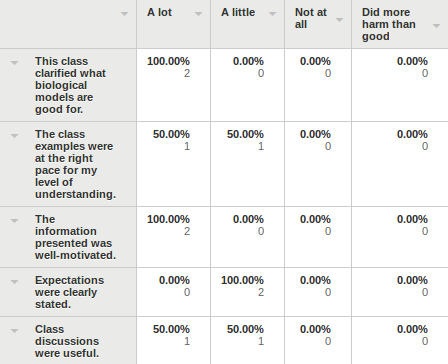
\includegraphics[width=0.8\hsize]{workshop/table_of_responses.png}
	\caption{Responses from student survey.  Only 2 of 5 students replied.} 
	
\end{figure}

\paragraph{What are some questions you have about biological modeling that this class should have addressed.}

I think it might be good to emphasize presentation and interpretation of modeling results, both from the perspective of the experimenter and the reader. In other words, I think it would be good for people to become comfortable both reading theoretical papers and generating simple modeling figures. I know this wasn't the focus of the workshop, but it might be nice to briefly cover agent-based modeling to the point where someone could be conformable interpreting experiments. 

It was a good foundation. Maybe how to interpret a model in a paper and evaluate it, if we did an example in class that would be helpful. 

\paragraph{ Describe how you would like to see this workshop structured to best promote your learning of the material }

It might be a good idea to have a list of things to model, so that people can still progress through the workshop even if the system they work on isn't amenable to modeling or isn't interesting to model. I liked the emphasis on students giving short presentations throughout. 

A little more background on the basic calculus we needed. Also talking more about the reasoning behind what you're doing and less algebra on the board, it's kinda hard to follow but we can all probably do it. 




\section{Reflections and Future Ideas}

In general, the students reacted positively to the framework that we established with it's emphasis on the three C's outlined above.  The student survey responses showed that the focus on classroom participation was welcome.  In practice, the students were not required to complete any homework, and the course was not given for a grade.  This led to many of the assignments being neglected entirely.  However, despite all of the work being completely optional, many of the students completed a significant portion of the work voluntarily.  

In the future, I will need to do a bit more preparation work to select a larger corpus of example systems for students to work with.  And having more examples to work through together will also probably improve outcomes. On the other hand, I don't want to lose the student driven focus that I was hoping to attain. I may also want to establish a bit more authority so that students attend class with their assignments completed.   


\section{Course Materials}

The course slides are available online at the following URL:

https://drive.google.com/drive/folders/0B3gBL61483U8Z2h1b3JRUHZMQ1k?usp=sharing

Below you can find the Q\&A material used for quizzes or discussion prompts.


\subsection{How mathematical models make sense of complex processes}

% 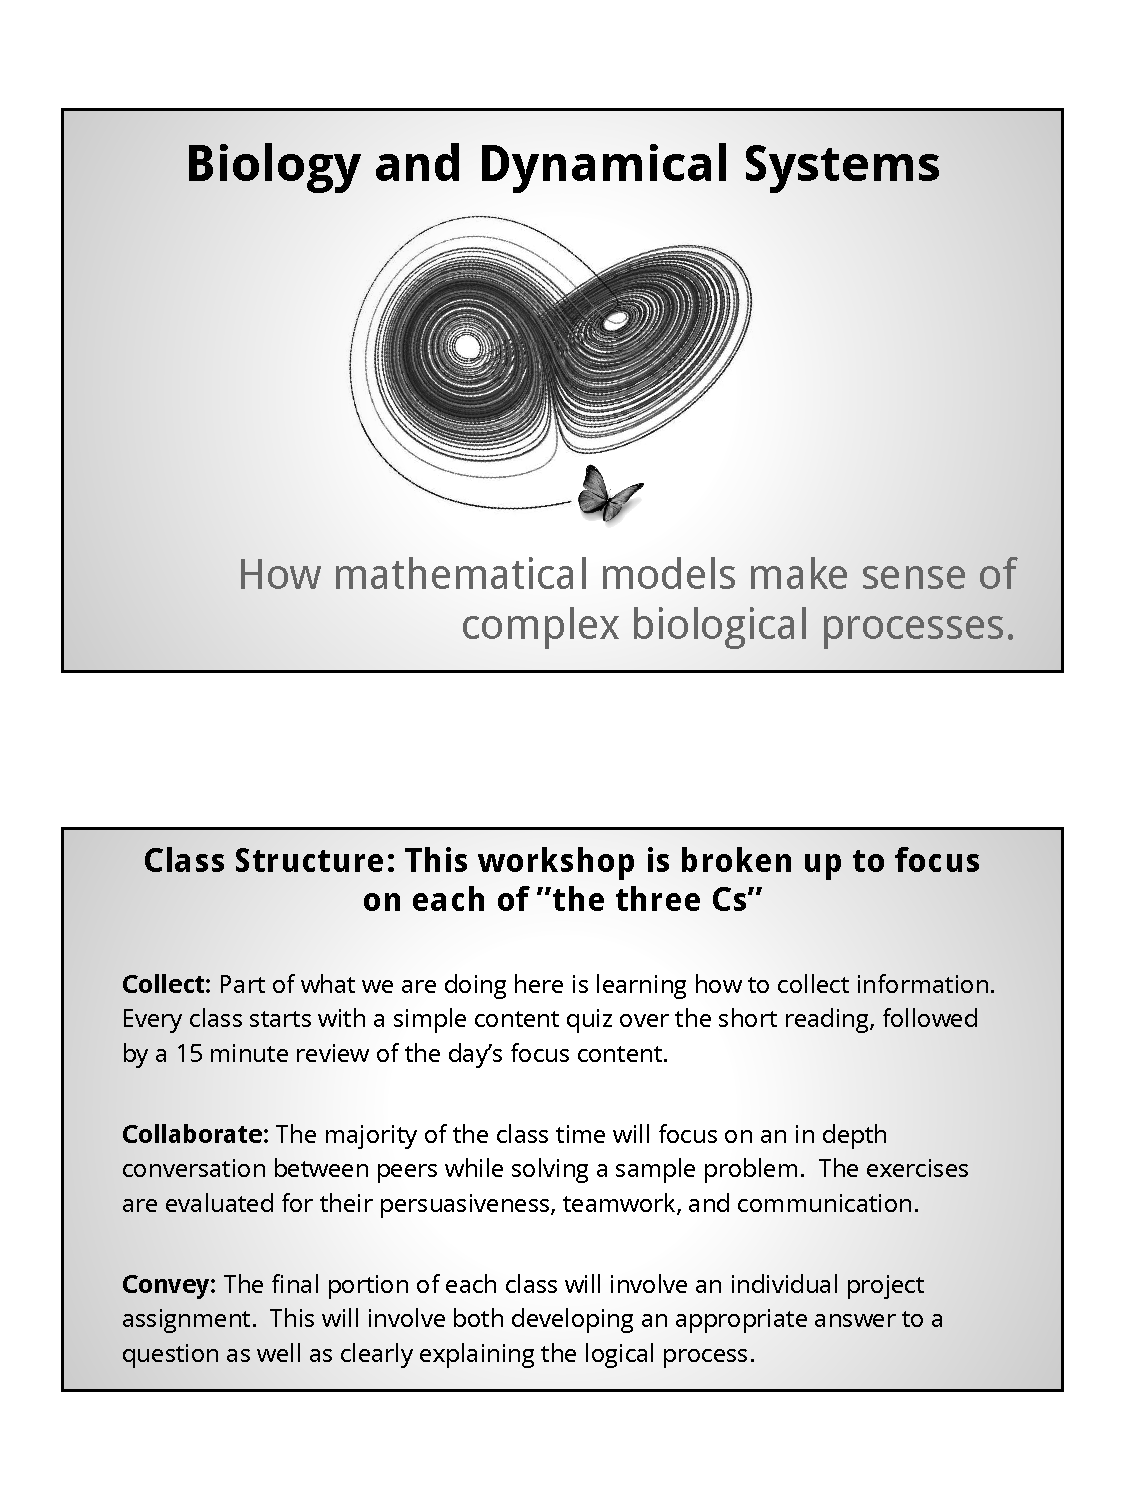
\includepdf[pages={1-}]{workshop/wk1_intro_and_cartoons.pdf}


\subsection{Modeling biological systems with differential equations}
\paragraph{Modelling biological systems} is a significant task of systems biology and mathematical biology. It involves the use of computer simulations of biological systems, including cellular subsystems (such as the networks of metabolites and enzymes which comprise metabolism, signal transduction pathways and gene regulatory networks), to both analyze and visualize the complex connections of these cellular processes.'' --Wikipedia

\paragraph{Many types of models} Biological models can work in many different ways:  In general, models are made to focus on systems at a certain scale.  We can choose from a wide variety of model types. Some work by modeling continuous values, such as concentration of a protein.  Others work by modeling the discrete state of a system, such as a neuron being either on or off.  Some models are deterministic, meaning that there is no randomness, while others add stochastic noise.

\paragraph{Focusing on Differential equations} In our class we're going to focus on probably the simplest and most widely used kind of mathematical model, differential equations.  Differential equations are a continuous, deterministic model, they model real values with rules that describe exactly how those values change.  Differential equations are very similar to the equations we learned about in our high school and college calculus courses.

\paragraph{What is a differential equation good for?} A differential equation is a simple formula that describes how a system will change in time based on the state of the system right now. You can think of it like a very formal protocol for how concentrations of substances will change over time.  For example, a differential equation 

% 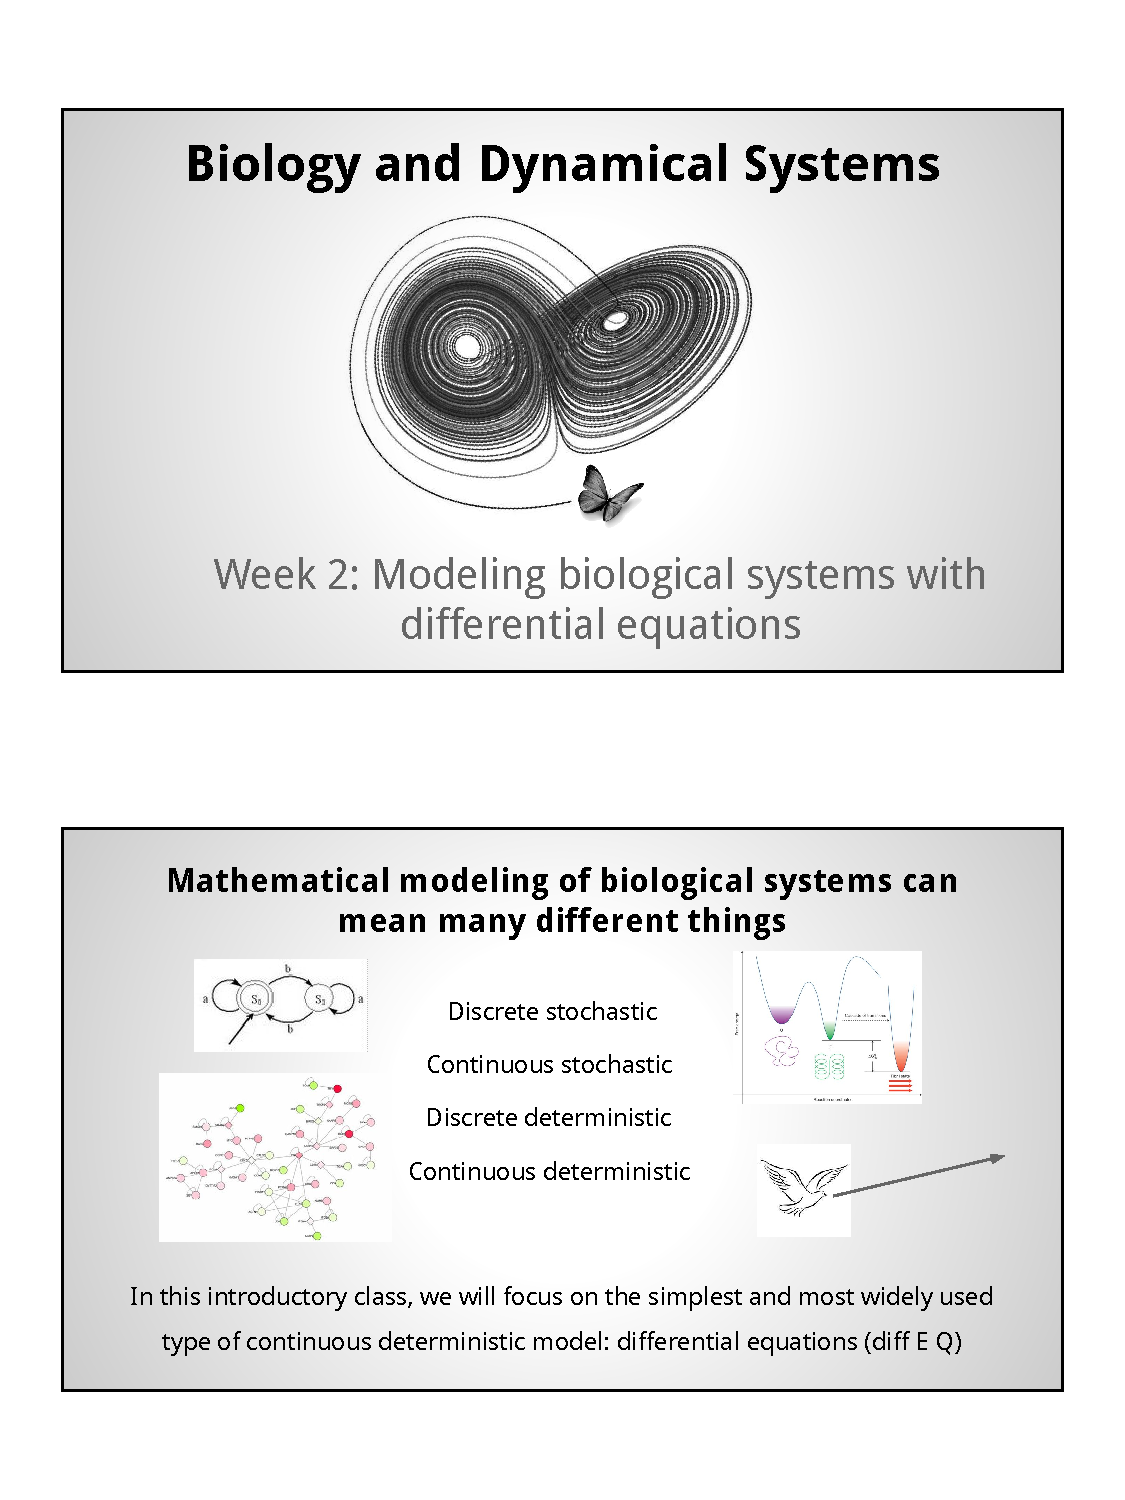
\includepdf[pages={1-}]{workshop/wk2_diff_eq.pdf}



\subsection{Visualizing equations with graphs}
\paragraph{Why is it called differential?} One could argue that differential equations could actually be called derivative equations.  That's because the equation itself is really just a way of explicitly writing out the derivative of a variable.  For those that don't remember a derivative is just a way to represent rate of change, that is - the amount by which a function is changing at one given point. It is also the slope of the tangent line at a point on a graph

\paragraph{Equilibrium?} Another important concept in diffeq is that of equilibrium.  The meaning of equilibrium is simple once you have a rate equation to look at.  When the net rates of change of all variable are equal to 0, then nothing can change anymore.  The rates of production and destruction are balanced, and the concentrations of everything will remain constant forever.  Not all systems reach equilibrium, but most do, and finding equilibria is the first step to understanding how many systems work.  We will use equilibrium and steady state more or less interchangeably though there are subtle, pedantic differences.

\paragraph{Initial conditions and transient behaviors} Even though most systems reach equilibrium after a long time, the system's initial conditions set the early transient behavior. The initial condition, or seed value, is simply the state of the system where we choose to start.  The transient behavior is the way in which the system changes from the initial conditions to the steady state.

\paragraph{What are nullclines?} If our rate equation has two variables that can change in it (i.e. not constants), then there is no longer a single value at which the rate equation will equal 0.  Instead there will be a set of values that make the rate 0.  This set of values defines a line, and this line is called a nullcline. 
% 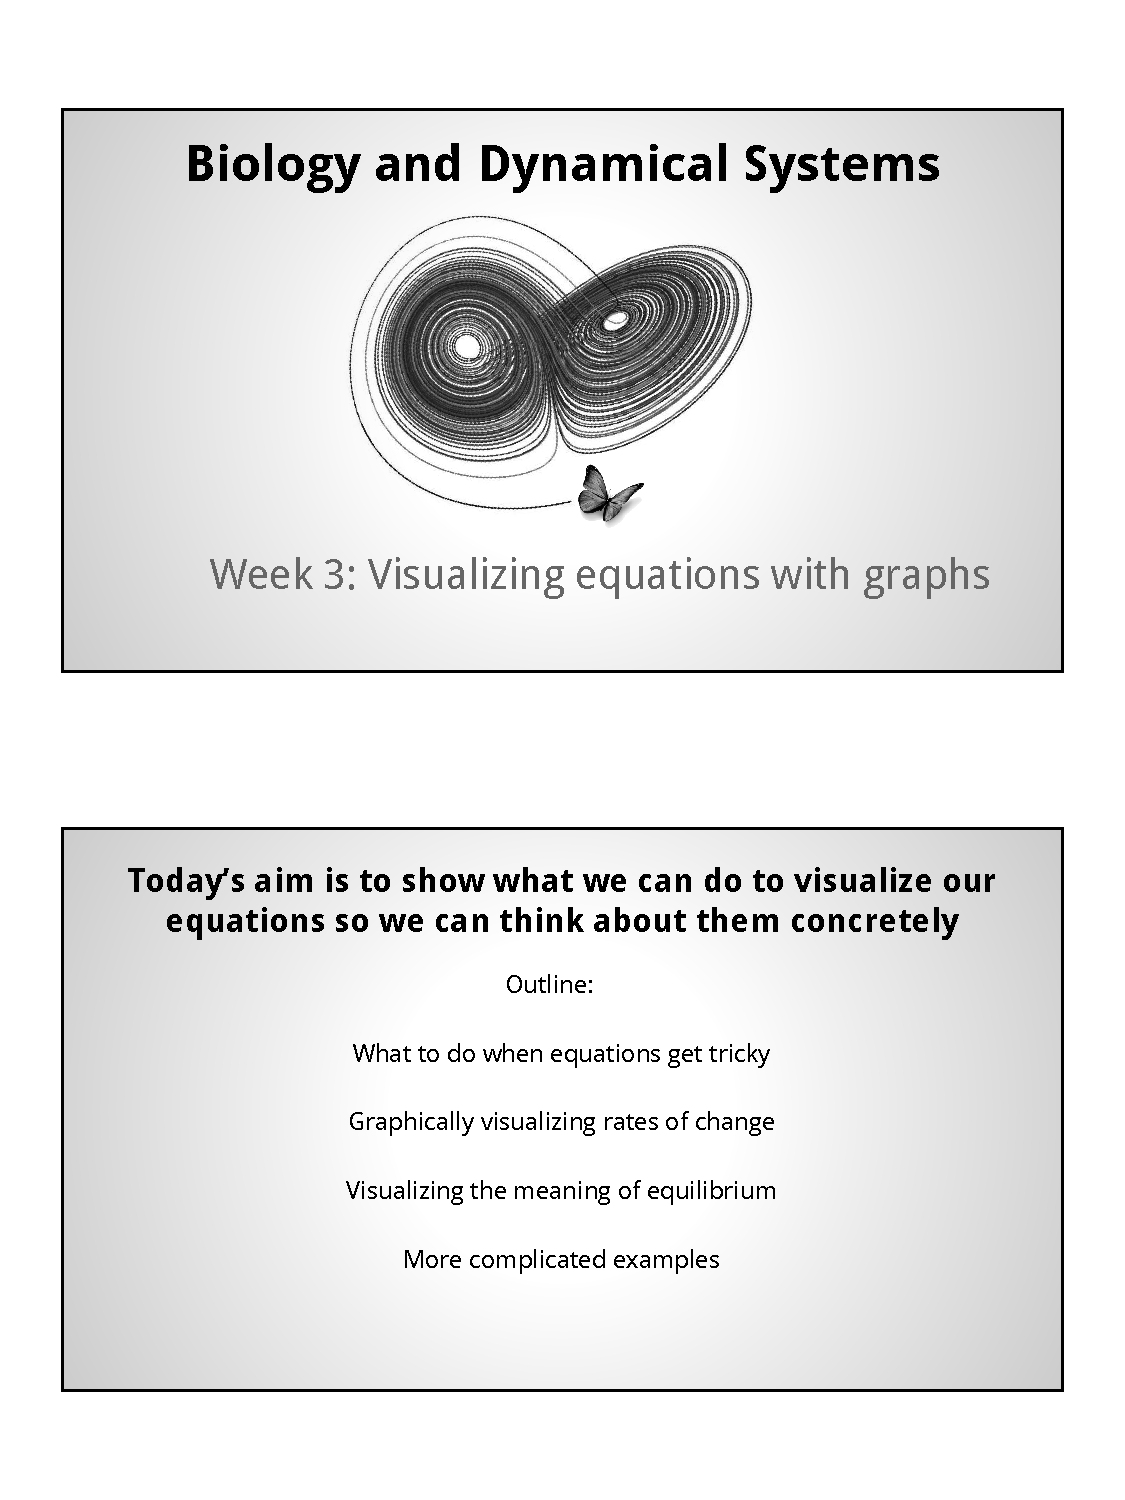
\includepdf[pages={1-}]{workshop/wk3_diag.pdf}



\subsection{Simplifying models and starting simulations}
\paragraph{Why simplify before simulating?} There are a number of reasons to simplify your equations before you ever start a simulation.  Here are my top three.  
1) You won't be able to remember or adequately describe all the parameters that went into a given simulation when somebody asks you.  If you have 20 parameters in a simulation there will always be a huge risk that you screwed one of them up and you will never be able to notice.  
2) If you want to understand how your model works under many different conditions, then every time you add a parameter you have to do exponentially more work.  In other words, when you are systematically checking how 3 parameters work together you may have to do $100^3$ different simulations and analyze your results.  If you add one more parameter you will have to do $100^4$ simulation or 100 times more work.  
3) Nobody wants to look at a disorganized giant equation.  If you have a complicated equation most people will decide it isn't worth their time to pay attention to the modeling so none of your modeling work will count for anything anyway.

\paragraph{The parts of a differential equation model} A differential equation model can be broken down into 3 parts: variables, parameters, and the form of the equation.  Variables are the values (like concentration) that are changing in time.  This is the physically 'real' stuff like the number of proteins or the size of your cell.  Parameters are things like rate constants and diffusion coefficients.  These are descriptive numbers that set the magnitudes of rates of change.  Finally, the form of the equation determines how the variables and parameters fit together.  This is the level at which we can see how each variable affects the other qualitatively, but it takes parameters to know by how much.

\paragraph{How do simulations work?} The applied math behind solving differential equations with computers is rich and we certainly won't understand everything that has been done over the past 70 years to solve these problems.  However we can get some intuition by looking at the simplest way of solving, called the Euler method.  In this method you step through time and change the value of your variables by a small amount using the rules defined in your differential equation (See wikipedia page for more info).  If you ever try this, you will get bored very fast because it is really annoying.  But when computers do this, they can take very small steps and therefore solve the system with arbitrary accuracy.  There have been a bunch of modifications of this technique that significantly improve the accuracy vs timestep tradeoff.


% 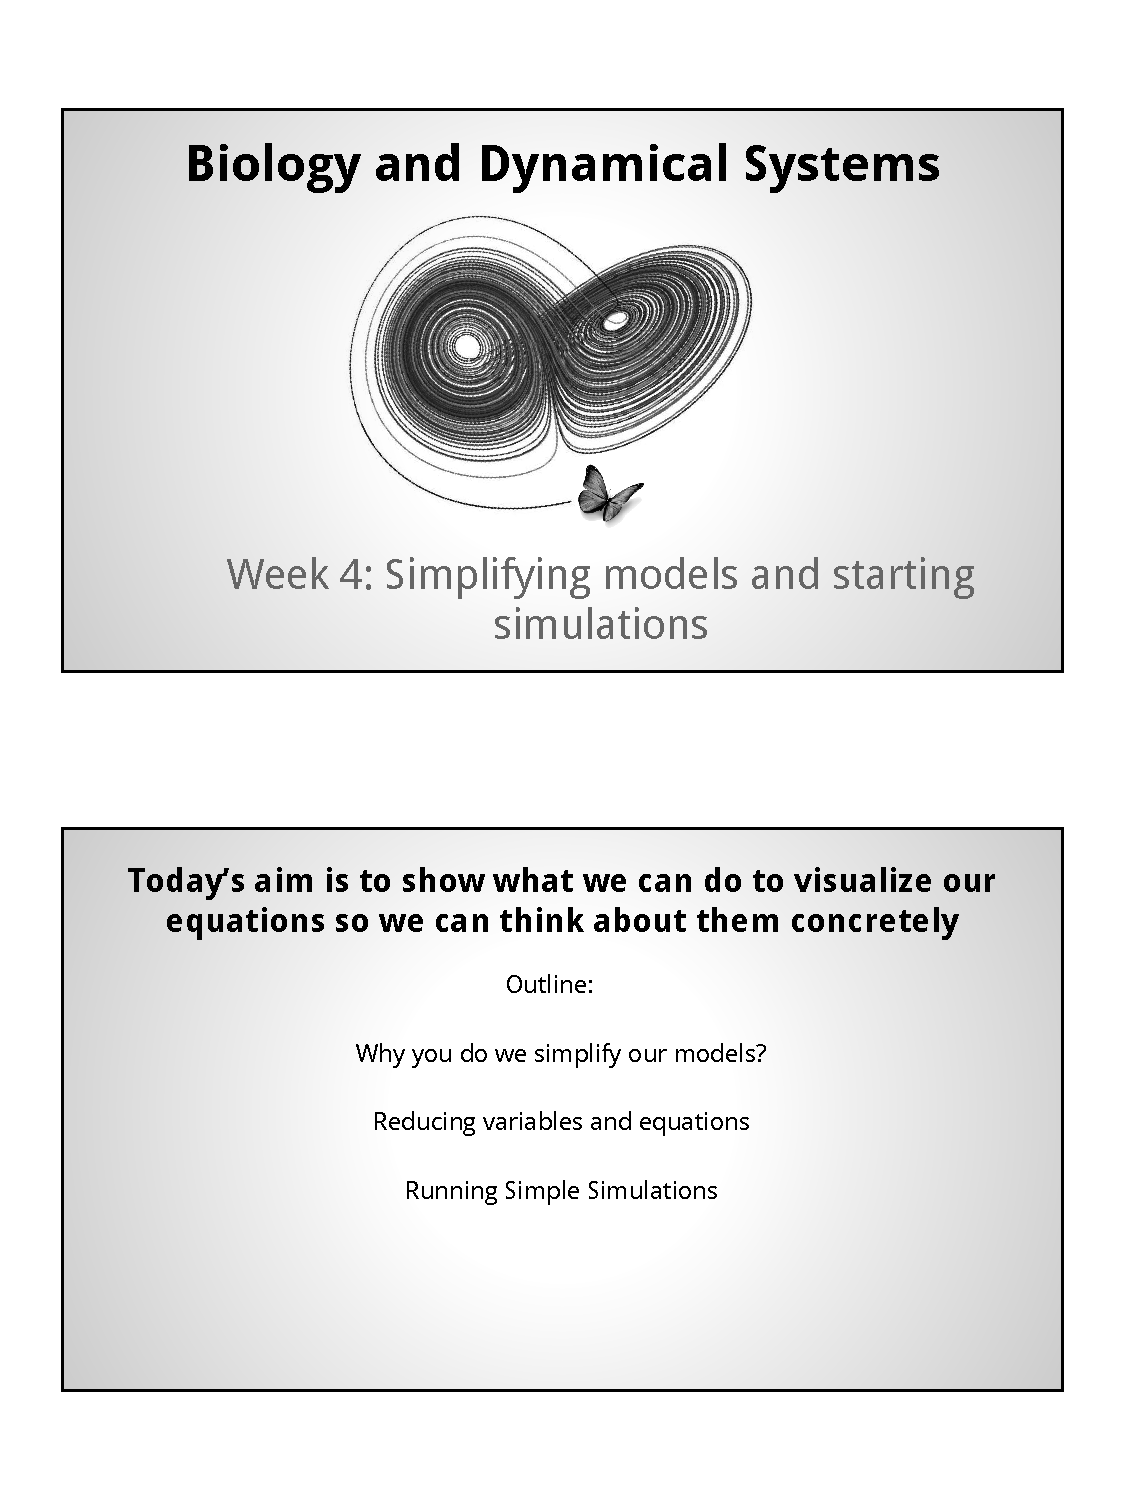
\includepdf[pages={1-}]{workshop/wk4_simple.pdf}



\subsection{Analyzing equations and understanding simulation output}

\paragraph{(from wikipedia) Nondimensionalization} is the partial or full removal of units from an equation involving physical quantities by a suitable substitution of variables. This technique can simplify and parameterize problems where measured units are involved. It is closely related to dimensional analysis. In some physical systems, the term scaling is used interchangeably with nondimensionalization, in order to suggest that certain quantities are better measured relative to some appropriate unit. These units refer to quantities intrinsic to the system, rather than units such as SI units. Nondimensionalization is not the same as converting extensive quantities in an equation to intensive quantities, since the latter procedure results in variables that still carry units.

\paragraph{Running simulations}: The following two snippets of code is all you need to solve differential equations in MATLAB.


\begin{verbatim}
function dc = myode(t,p,a,b)
    p1 = p(1);
    p2 = p(2);
    dp1 = 1 - a*p2 - p1;
    dp2 =p1 - b*p2;
    dp = [dp1;dp2];
end
\end{verbatim}

\begin{verbatim}
t = 0:0.1:10;      #timepoints for solution (1 to 10 increment of 0.1)
p0 = [1,0];         #initial conditions for the concentration of p1 and p2
a=1; b=1;          #optional constants a and b which will change behavior
[t, pt] = ode45(@myode,t,p0,[],a,b);        #this runs the simulaton 
plot(t,p(:,1)); hold on; plot(t,p(:,2));           #this plots the output
\end{verbatim}

So now you can put whatever you want into the equation and change your parameters and run many simulations.  

% 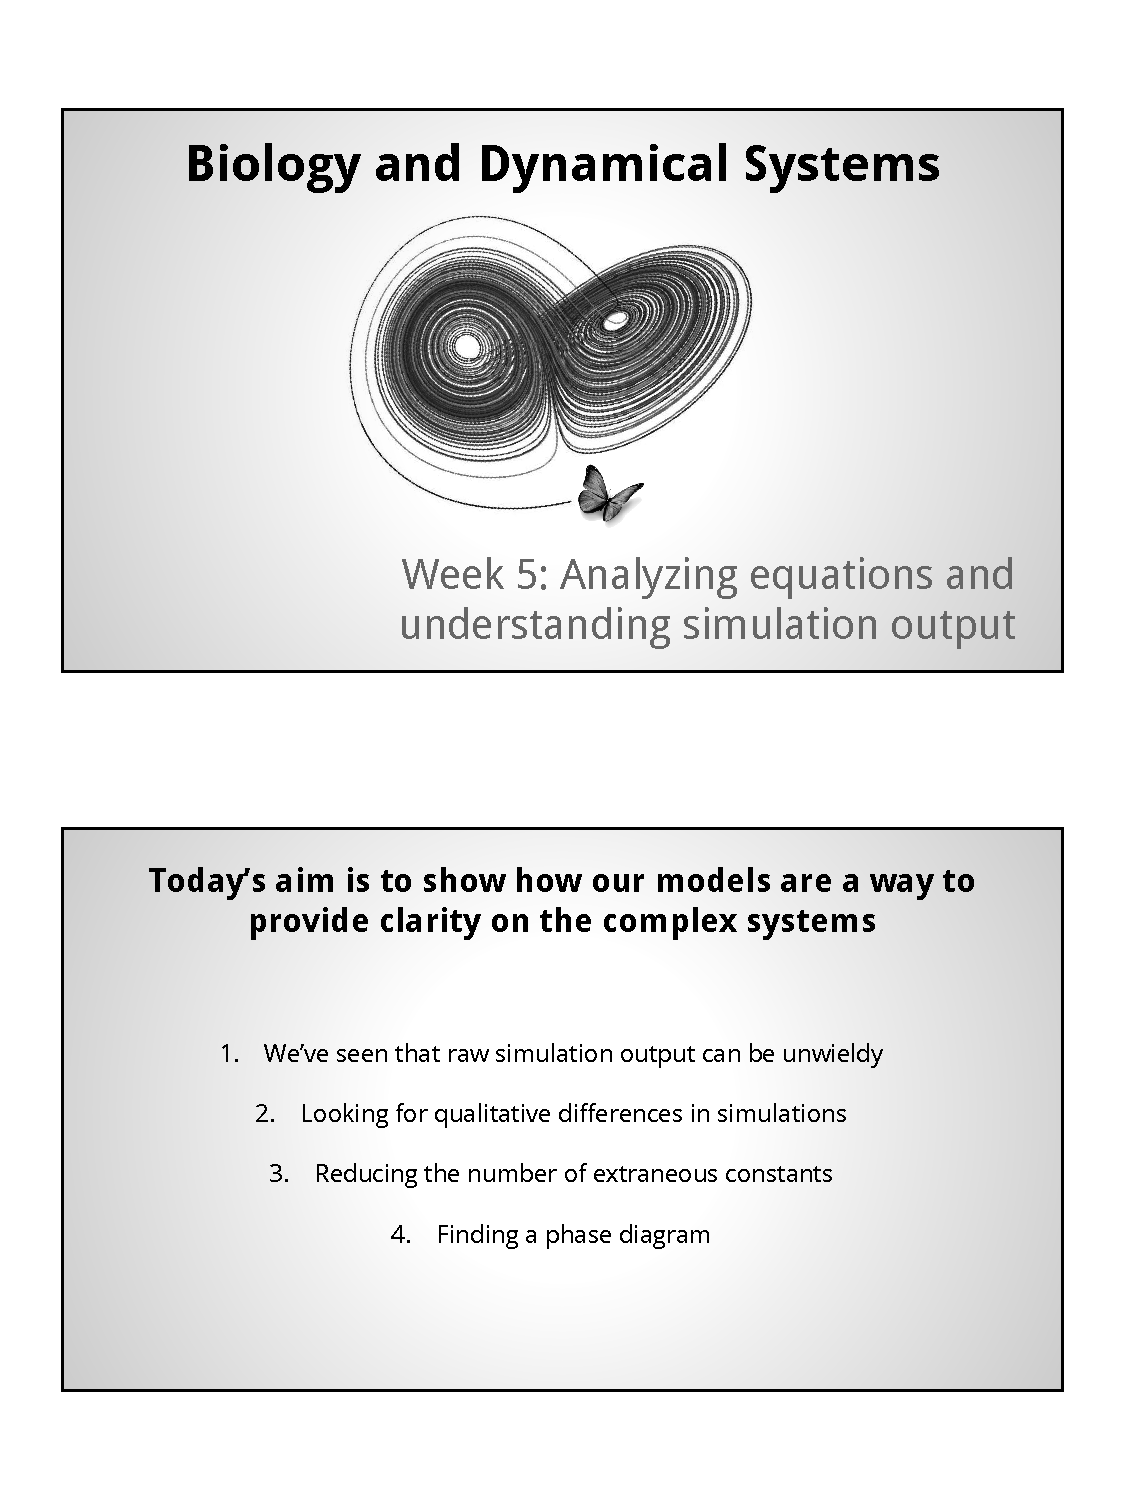
\includepdf[pages={1-}]{workshop/wk5_analysis.pdf}



\subsection{Explaining ever more complex systems}

% 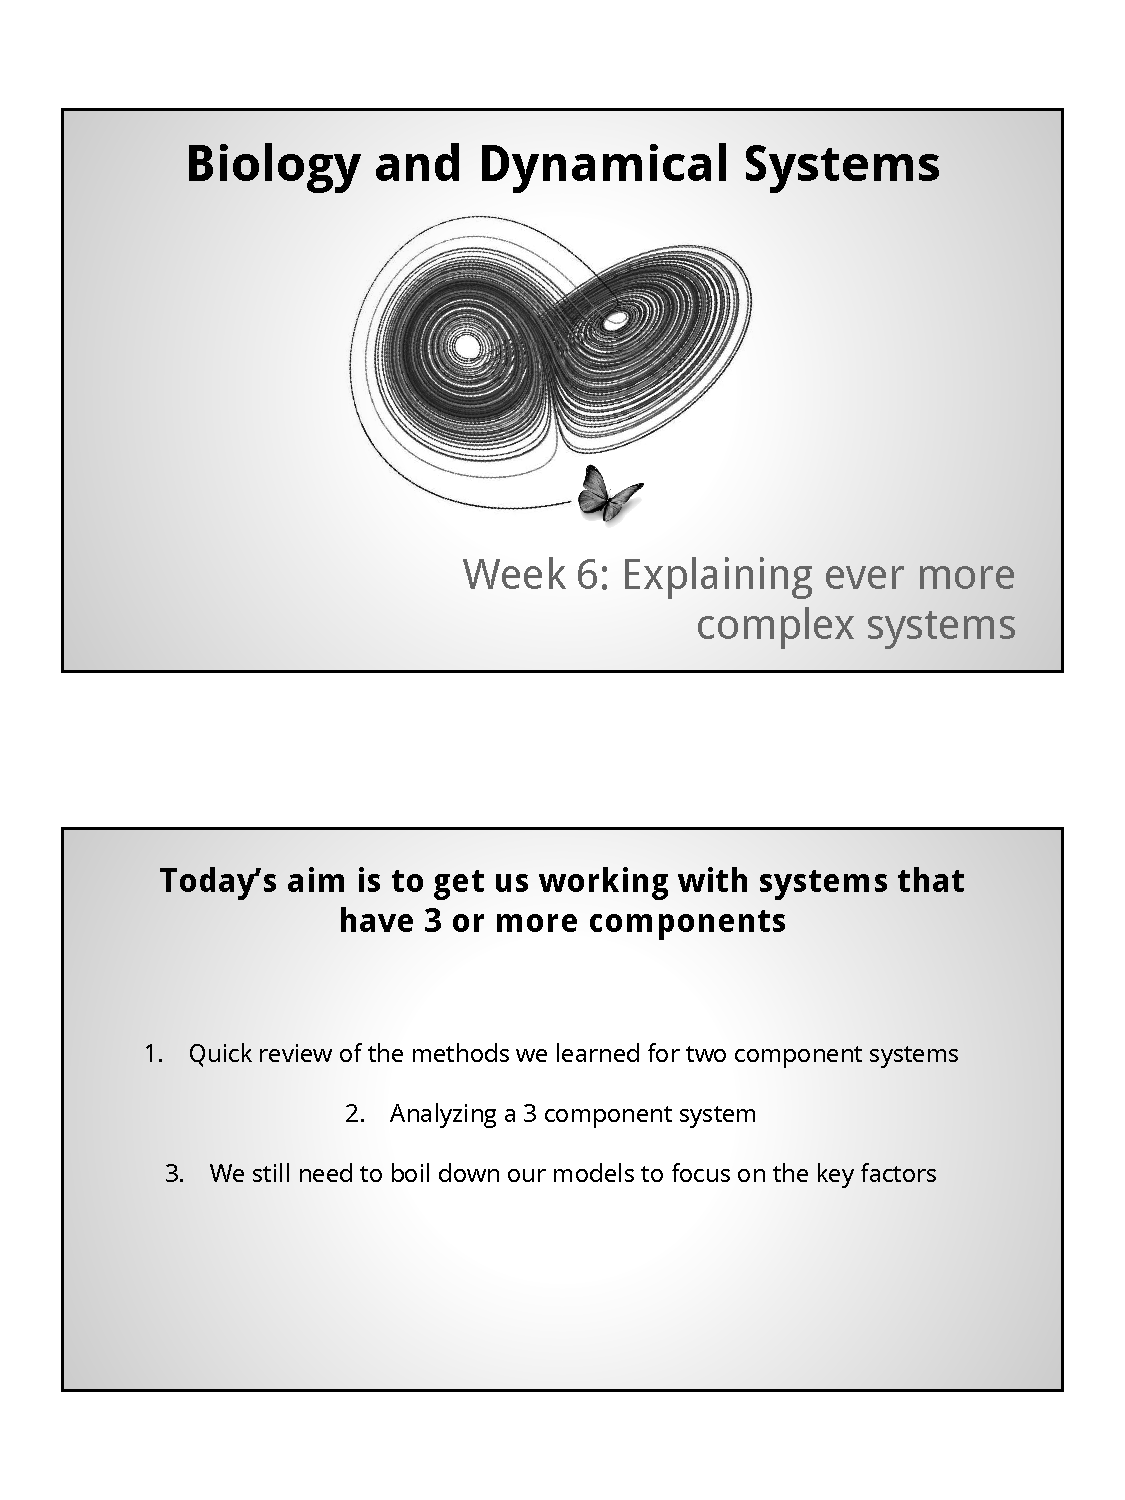
\includepdf[pages={1-}]{workshop/wk6_display.pdf}


\section{Quizzes and Project ideas}
\paragraph{W2}
Q1: Which is not a situation that is amenable to mathematical modeling?
A metabolism, signal transduction pathways, gene regulatory networks, protein purification

Q2: Which is a category of biological mathematical model?
A soft, prescient, discrete, topological

Q3: Which type of model is a differential equation?
A continuous deterministic, discrete stochastic, continuous stochastic, discrete deterministic

Q4: What does a differential equation most closely resemble?
A a protocol, a patent, a dissertation, a legume


\paragraph{W3}
Q1: Which is the closest synonym for derivative in the context of diffeq?
A Unoriginal, by-product, change, sum

Q2: Which is least similar to equilibrium?
A balanced rates, constant concentrations, discrete probabilities, steady states

Q3: Which conditions set the transient behavior?
A initial, parametric, hyperbolic, final

Q4: Nullclines are...
A topographical, unimportant, lines, esoteric

\paragraph{W4}
Q1: Number of simulations to run varies --- with the number of free parameters.
A quadratically, logarithmically, exponentially, combinatorially

Q2: Which is not a part of a differential equation model?
A definitions, variables, parameters, the form of the equation

Q3:The Euler method gives exact solutions.
A True, False, neither, depends who you ask

Q4: Who likes looking at a disorganized mess of an equation?
A Your PI, your colleagues, your reviewer, nobody

\paragraph{W5}
Q1: Once nondimensionalization is complete?
A All variables have units of time, there are no more parameters left, equations are simpler to analyze, your solutions will fall on a line

Q2: In MATLAB --- is the function for solving differential equations
A ode23tb, ode113, ode45, ode15i

Q3: Which isn't necessary to solve a differential equation
A An ode function, constants, initial conditions, timepoints for solution


\chapter{Reducing power consumption in High Performance Computing}


\section{Introduction}

Data centers in the US consume an estimated 91 billion kilowatt-hours yearly, equivalent to the annual output of 34 large coal-fired power plants.\cite{Delforge2014} These same estimates show that only 6-12\% of the electricity is used for powering servers while the rest is used to keep machines idling, wasting resources and money in the process. Data center electricity is not inexpensive, costing American businesses \$13 billion annually in electricity bills.\cite{Delforge2014} Because cost is a strong motivating factor for businesses and universities, we consider data center energy efficiency in the context of cost savings for data center operations. \\

\begin{figure}[t]
	\begin{center}
		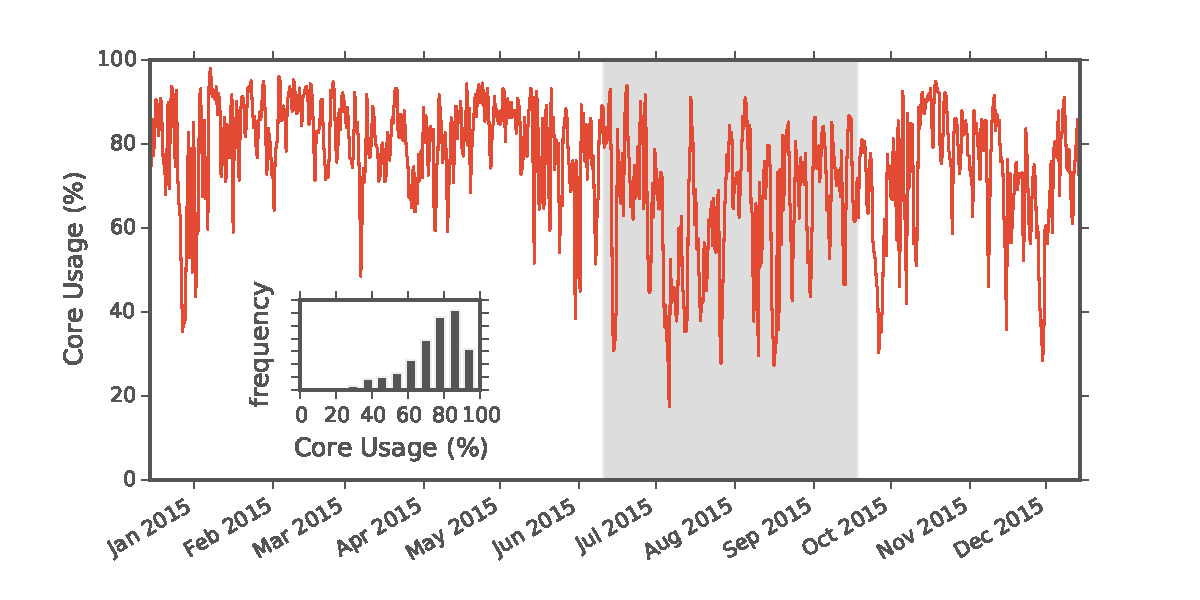
\includegraphics[scale=0.38]{edeals/pwr_model_ins}
		%		\begin{picture}(300,150)(0,200)
		%		\put(-15,-30){\special{psfile = fig1.ps hscale = 50 vscale = 50}}
		%		\end{picture}\\
	\end{center}
	\caption{Average core usage for a 244 node shared HPC partition in the Midway cluster. Insert shows usage statistics histogram.}
	\label{prw_model_ins}
\end{figure}

Demand response (DR) programs provide incentives to induce dynamic management of customers’ electricity load in response to power supply conditions, for example, reducing their power consumption in response to a request from the utility.\cite{7039172} Anita can you add something around here that points out how demand response also increases the “sustainability” of the datacenter beyond just cost reduction.Many energy providers have Voluntary Load Response (VLR) programs, which encourage commercial consumers to reduce power demands during peak periods, such as particularly hot summer days. Participants are given between one and four hours’ notice of a request to shed some of their electric load, with two and eight hours of participation and the expectation to shed at least 10 kilowatts. We are interested in exploring more active ways in which to participate in electricity demand response programs while impacting the users minimally.   \\

In many university data centers, a significant portion of the data center is dedicated to high performance research computing which is typically Tier 1. While these jobs take longer periods of time to complete, they are less time sensitive and more flexible than systems which support core business functions such as the university's email.  We wish to use the flexibility in scheduling of these jobs to reduce energy consumption of university data centers during periods of peak energy demand. \\  

As shown in the example core usage data of Figure \ref{prw_model_ins}, although the typical average usage during the school year is a fairly standard 80\%, the averaged workload can fall to 65\% of full capacity in the hottest summer months from June to September. These months also present the period of greatest electricity demand due largely to increased usage of air conditioning. This presents a valuable opportunity to potentially curtail electricity use in demand response scenarios by shifting load off of the peak periods of energy price.  Toward this aim, this paper is our attempt to estimate the economic savings, feasibility, and any potential user impact from full or partial cluster shutdown during periods of increased energy demand.


\subsection{Alternative Demand Response Options in Data Centers}

Although we focus on load shifting for our study, we wish to point out prior work on alternative strategies for demand response. \\

\textbf{Facility changes} A study by Lawrence Berkeley National Laboratory (LBNL) found that 5\% of the data center load can typically be shed in 5 minutes and 10\% of the load can be shed in 15 minutes without changes to how the IT workload is handled, i.e., via temperature adjustment and other building management approaches\cite{Ghatikar2012}. Most data centers have local power due to a backup generator, which could also be used to absorb some load during peak time \cite{Liu2013}. More recently, methods of energy storage have been proposed\cite{Narayanan2014} in which UPS batteries are re-purposed for provisioning during periods of peak demand in addition to their primary purpose of backup power. However, these methods all entail manual intervention, with close monitoring and control.

\textbf{Power capping} is a strategy by which to run data center equipment within a set of constraints which assume the electricity draw for the data center as a whole cannot grow any larger. Some examples of this include and turning off or constraining CPU/GPU power consumption to values below the CPU Thermal Design Power (TDP) value, which requires less voltage. Many equipment manufacturers - including IBM, Intel and AMD - have implemented power capping technology that can be monitored at the processor level and applied at the rack level. One approach to power capping is Dynamic Voltage/Frequency Scaling (DVFS). However, as noted by Roundtree\cite{Roundtree2012}, no machine in the Top 500 list of supercomputers makes use of DVFS to save power or energy since the performance impact and the amount of power and energy saved was highly application dependent. Power capping doesn’t necessarily equate to energy efficiency nor cost savings.

\textbf{Schedulers} Zhou et al\cite{Zhou2014} present a method for power-aware scheduling by using a combination of a scheduling window and 0-1 knapsack model, which shows promise. However, since SLURM is our scheduler, we decided to focus solely on SLURM. Bodas et al\cite{Bodas2014} demonstrate an integration of power capping into a power-aware scheduler, with the overall goal of maintaining average system power within a budget. Their work demonstrates that SLURM’s auto mode can be used to maximize available power.  

\begin{figure}[t]
	\begin{center}
		
				\begin{picture}(300,100)(20,200)
				\includegraphics[scale=0.50]{edeals/ray_fig}
				\end{picture}\\
	\end{center}
	\caption{Energy monitoring framework.}
	\label{ray_fig}
\end{figure}


\section{Problem Statement}

Can load shifting of high performance computing tasks save universities money in energy demand response scenarios?  To explore the relative costs of implementing load shifting in demand response scenarios, we have expressed the problem by modeling total dollar cost.  We wish to use this framework to explore the optimization of price in the presence of various data center usage statistics and price fluctuation schemes.

\subsection{Modeling Energy Costs}

We generate a model total cost function composed of a fixed cost for purchasing and maintaining nodes plus a variable cost dependent on data center power usage and energy prices.  We wish to minimize the cost function

$$C = p_n T n_{max} + \int_0^T dt \cdot p(t)\left (n(t)u(t)+ u_w \frac{\Delta n(t) }{\Delta t} \right )  $$

where $p(t)$ is the price of power at time $t$, $0<n(t)<n_{max}$ is the number of running nodes, $u(t)$ is the average node power usage, $u_w$ is the wasted power from turning on a node, $p_n$ is the amortized lifetime cost of purchasing a node, and $n_{max}$ is the total number of nodes in the cluster.  

Based on our cluster usage statistics, we approximate that compute cycles are roughly interchangeable and that the main determiner of power usage is simply the CPU utilization of the node. In this case, node power usage takes the form

$$u(t) = u_0 + u_v \cdot r(t)$$

where $0<r(t)<1$ is the fraction of CPU usage, $u_0$ is the cost of an idling node and $u_v$ is the variable cost for doing $r$ work on a machine.

We wish to minimize the cost function $C$ subject to the constraint that the sum of the submitted CPU cycles, $S$, are all completed after a period T.

$$\int_0^T dt \cdot n(t)r(t) = S$$

\begin{figure}[t]
	\begin{center}
		\includegraphics[scale=0.55]{edeals/usage_viz4}
		%		\begin{picture}(300,150)(0,200)
		%		\put(-15,-30){\special{psfile = fig1.ps hscale = 50 vscale = 50}}
		%		\end{picture}\\
	\end{center}
	\caption{Diagram of job scheduling during a four node temporary shutdown experiment. Each colored rectangle displays the execution time of a single LAMPPS test job running for approximately 5 minutes.}
	
\end{figure}

\begin{figure}[t]
	\begin{center}
		\includegraphics[scale=0.55]{edeals/power_viz}
		%		\begin{picture}(300,150)(0,200)
		%		\put(-15,-30){\special{psfile = fig1.ps hscale = 50 vscale = 50}}
		%		\end{picture}\\
	\end{center}
	\caption{Total power consumed during experiments where variable numbers of machines were shut down during simulated peak pricing.}
	\label{power_viz}
\end{figure}

\subsection{Response to a Temporary Price Spike}

In particular, we wish to use this framework to determine how to run our data center in the situation where every $T$ days, we see a "price spike" from $p_0$ to $p_s$, lasting time period $t_s$.  This condition is highly similar to the one facility managers face when utility provides impose usage tariffs during peak energy demand periods.

In this situation, the number of running machines will change stepwise between a high number of running machines, $n_H=n_{max}$, and a low number of running machines, $n_L$, and a high and low CPU utilization $r_H=1$, $r_L$, with a corresponding $u_H$ and $u_L$ as defined above.  The high usage will occur during the cheap energy supply, and the low usage will occur during the price spike.  Therefore we can rewrite our cost function as 

\begin{equation}
	C = p_n n_H T + p_0 (u_0 + u_v) n_H (T-t_s) + p_s (u_0 + u_v r_L) n_L t_s + p_0 u_w (n_H-n_L)
\end{equation}

with the constraint

\begin{equation}
n_H (T-t_s) + n_L r_L t_s = S
\end{equation}

Inserting the constraint into our cost function to replace $r_L$ yields 

\begin{equation}
C = p_s u_v S + n_L \cdot( p_s u_0 t_s - p_0 u_w t_w) + n_H \cdot (p_n T + p_0 u_w t_w -(\Delta p u_v - p_0 u_0)(T-t_s))
\end{equation}
where we've introduce the price difference, $\Delta p = p_s - p_0$.

We can analyze the change in costs as a function of $n_L$ and $n_H$ to determine the optimal cluster setup for known variables, $t_s$, $p_s$, $p_n$, $p_0$, $u_0$, $u_v$, and $u_w$. 

From this analysis, whenever $ p_s u_0 t_s < p_0 u_w t_w$, the cost of powering off nodes exceeds the cost of running those nodes idle so $n_L = n_H$ and $r_L = S/n_H t_s - (T-t_s)/t_s$. Otherwise powering off nodes saves money so the nodes that remain on run at full capacity $r_L = 1$, and $n_L$ is minimized subject to constraints giving $n_L = S/t_s - n_H(T-t_s)/t_s$.

If we can freely choose $n_H$ to optimize cost, then whenever $(\Delta p u_v - p_0 u_0)(T-t_s) > p_n T + min(p_0 u_w t_w,p_s u_0 t_s)$, we would increase $n_H$ (i.e. buy more machines) until all the work is done during the cheap energy period. Therefore $n_H = S/(T-t_s)$ and either $n_L$ or $r_L$ is $0$.  Otherwise, the cost of new machines is more than any cost savings achieved from exploiting the price difference, and we would simply ignore the price spike (i.e. set $n_H = n_L = S/T$ and $r_L = 1$).

% you can also use the wonderful epsfig package...
\begin{figure}[t]
	\begin{center}
		\includegraphics[scale=0.55]{edeals/down_v_pow}
		%		\begin{picture}(300,150)(0,200)
		%		\put(-15,-30){\special{psfile = fig1.ps hscale = 50 vscale = 50}}
		%		\end{picture}\\
	\end{center}
	\caption{Energy usage of test cluster during partial shutdown experiments.  Solid lines indicate power usage during the shutdown, while dashed lines indicate power usage after returning to full operation.}
	\label{down_v_pow}
\end{figure}

% you can also use the wonderful epsfig package...
\begin{figure}[t]
	\begin{center}
		\includegraphics[scale=0.55]{edeals/down_v_wait}
		%		\begin{picture}(300,150)(0,200)
		%		\put(-15,-30){\special{psfile = fig1.ps hscale = 50 vscale = 50}}
		%		\end{picture}\\
	\end{center}
	\caption{Maximum (solid) and mean (dashed) job wait times during partial shutdown experiments.}
	\label{down_v_wait}
\end{figure}

\section{EDEALS: Electricity Demand-response Easy Adjusted Load Shifting}

For a data center manager to use the above model to determine their cost savings, they must collect and analyze usage and power data on their system.  We have built a cluster data processing pipeline, EDEALS, to assess the magnitude of potential savings available from a full or partial cluster shutdown.  We combine SLURM job scheduling, node level IMM power and usage metrics, and cabinet level CDU measurements to determine the optimum magnitude of demand response cluster shutdowns.  

Here we describe our data center instrumentation, so that we ensure accurate measurements of performance of the workload management system and HPC cluster alone without the influence of extraneous components. Since our focus is the HPC cluster and SLURM manager, we need to ensure those components alone affect the reduced data center utility bill.  As depicted in Figure \ref{ray_fig}, we take measurements at the core, node, rack, and cabinet level.  These data are combined to detect power losses at each step and to determine the correlation between the power measurements at the machine level and the true power draw at the facility level.

Combining this data with electricity pricing statistics from utility managers allows system administrators to determine when and by how much to reduce their power usage to save money.  We have built a set of scripts particular to our system to implement machine level power down in response to predicted energy peaks.  At the end of the peak energy period the machines automatically reboot and are added by to SLURM’s available server pool.  At this time, these power cycling scripts are manually executed by system administrators after evaluation of the likelihood of near-term energy demand peaks.  However, as more data centers begin to implement smart metering, it will become possible to automate load shifting in response to real-time energy pricing indicators.  We look forward to continuing this as future work.





\section{Small-Scale Evaluation of EDEALS}

To test our load shifting scheme, we launched a series of small-scale experiments on a 6 machine test cluster using SLURM batch management system to schedule jobs. We wished to compare the energy savings and job wait times during a full or partial cluster shutdown in response to an energy price spike.

\subsection{Experimental Setup}

We measured the total energy use over a 3.5 hour window of which the first 30 minutes comprised a partial cluster shutdown, followed by a 15 minute powerup routine. We explored the impact of shutting down between one and all six nodes during the 30 minute window. The shutdown was carried out by fully powering nodes off.  We compared this to the energy usage without the partial shutdown.

Identical sample jobs were submitted to the cluster via SLURM scheduler at a constant rate to set the average cluster usage to approximately 55\%, 60\%, 65\% and 75\% capacity.  We used custom state control commands to set the power states of individual machines in the test cluster.  The SLURM scheduler automatically shifted queued jobs to run on the available machines, as shown in the example job schedule displayed Figure \ref{usage_viz} from a four node shutdown experiment. We used our EDEALS data analysis pipeline to measure the changes in energy usage and job wait time in the queue.

\subsection{Evaluation of Model Parameters}

Importantly, EDEALS allowed us to determine appropriate power parameters, $u_0$, $u_v$, and $u_w$ for both our test rack as well as a larger partition of the University of Chicago's Midway production cluster.  Figure \ref{pwr_proc} shows the measured relationship between CPU utilization and energy usage as determined from the machine level IPMI metric data.


\begin{figure}[t]
	\begin{center}
		\includegraphics[scale=0.55]{edeals/pwr_proc}
		\includegraphics[scale=0.55]{edeals/pwr_proc_c}
		%		\begin{picture}(300,150)(0,200)
		%		\put(-15,-30){\special{psfile = fig1.ps hscale = 50 vscale = 50}}
		%		\end{picture}\\
	\end{center}
	\caption{Power data for test cluster (top) and production cluster (bottom) nodes in presence of variable usage. The slope and intercept of the line are used to determine $u_v$ and $u_0$ respectively. }
	\label{pwr_proc}
\end{figure}

\begin{figure}[t]
	\begin{center}
		\includegraphics[scale=0.55]{edeals/ipmi_v_cdu}
		%		\begin{picture}(300,150)(0,200)
		%		\put(-15,-30){\special{psfile = fig1.ps hscale = 50 vscale = 50}}
		%		\end{picture}\\
	\end{center}
	\caption{Comparison between node level IPMI measurements and rack level CDU measurements. Best fit shows the model relationship used to convert IPMI data to estimated total power draw.}
	\label{ipmi_v_cdu}
\end{figure}

To account for losses not measured at the IPMI level, we compare the sum IPMI power usage to the rack level power monitoring.  This comparison revealed a correction factor of 1.25 between the IPMI measurement and the total rack level energy draw.  Using this corrected model, we were able to predict power consumption at the CDU level via CPU utilization under variable scheduler loads.

\subsection{Relative Energy Savings and Max Wait Times}

Our test cluster provided us with an important baseline in determining the effectiveness of a partial shutdown in reducing energy usage. As shown in Figure \ref{power_viz}, the total power draw from the test cluster was reduced dramatically during the shutdown period, and then returned to its baseline level.  

These experiments were repeated with different job submission rates such that the average CPU usage varied from 55\% to 75\%.  As shown in Figure \ref{down_v_pow}, the partial shutdowns reduced the total energy usage as measured at the CDU level.  Not surprisingly, the power usage during cluster shutdown for all usage levels converged to roughly the same value at the point where all remaining operational machines reached full capacity. Interestingly, the energy savings did not appear to be perfectly directly proportional to the fraction shut down.  In particular, there was residual energy use associated with our machine's low power state even when the cluster was entirely shut down.   

We also measured the difference between job submission and start time, as depicted in Figure \ref{down_v_wait}.  As one would expect, both mean and max wait times increased as the shutdown fraction grew and the effect was more pronounced when the cluster usage was higher.  However, we were pleasantly surprised to find that max wait times topped out at 45 minutes, which was the duration of the entire cluster down period.  This indicates that SLURM doesn't add too much additional overhead, and therefore, the worst-case user wait times would not exceed the total period that the cluster was shut down.

\section{Conclusion: Implication for An Operational HPC Datacenter}


In an HPC datacenter, the variable cost to supply electricity to a facility can be decomposed into both a nominal cost per kilowatt-hour and a procurement cost from the supplier.  Some suppliers impose a substantial procurement tariff based on electricity usage during the five, two hour long periods of highest demand in a year.  In this scenario, the savings of load shedding can be orders of magnitude higher than the nominal price per kilowatt-hour.  We estimate that by curtailing 1MW, 8 times per year, we can expect an annual savings of approximately \$100K, which in our case was roughly a 7% cost savings.  Approximating that the 8 curtailment days are roughly spread out over the 4 month period from June to September, we arrive at the system parameters listed in Table \ref{params}.



Combining these values with the power usage measurements from our production cluster, we can extrapolate the yearly savings based on fractional shutdowns of the data center.  In addition, using the wait time statistics from our test cluster we can also estimate the worst-case impact on user wait-times that these cluster shutdowns will incur.  We display this information in Figure \ref{final}, as a function of the fraction of the cluster that we would be theoretically willing to shut down.

\begin{figure}[t]
	\begin{center}
		\includegraphics[scale=0.5]{edeals/final}
		%		\begin{picture}(300,150)(0,200)
		%		\put(-15,-30){\special{psfile = fig1.ps hscale = 50 vscale = 50}}
		%		\end{picture}\\
	\end{center}
	\caption{Estimated savings from partial cluster shutdowns. }
	\label{final}
\end{figure}


\begin{table}[]
	\centering
	\label{my-label}
	\begin{tabular}{|l|l|l|l|}
		\hline
		\textbf{$T$} & \textbf{$t_s$} & \textbf{$p_0$} & \textbf{$p_s$}  \\ \hline
		360 hr & 2 hr & \$0.03/kWh  & \$6.5/kWh    \\ \hline
	\end{tabular}
	\caption{Model parameters estimated for medium scale HPC datacenter.}
	\label{params}
\end{table}

\section{Acknowledgments}

Special thanks goes out to Brandon for all his work getting our test cluster set up as well as for his useful input on machine pricing information.  We also wish to thank Matt Beach for his invaluable knowledge on energy pricing mechanisms and university power plans.  Finally, we wish to thank Dr. Birali Runesha for his support in carrying out this project.

\section{Availability}

On our Github, we have provided all data collection scripts, analysis routines, and experimental setups, as well as detailed calculations and optimization methods for other price models.  

\begin{center}
{\tt https://github.com/rcc-uchicago/datacenter}
\end{center}








\chapter{Source Code and Documentation}
\section{Finding Source Code Online}

Source code and up-to-date documentation are available online for the projects described in this dissertation.  

\begin{itemize}

\item https://github.com/wmcfadden/smPress
\item https://github.com/wmcfadden/activnet
\item https://github.com/munrolab/pulse-reaction-dynamics

\end{itemize}

%\subsection{Instructions for running MATLAB pre-compiled code}

%\subsection{Simulation Source}
% this line generates all the followings lines
% find . -name "*.m" ! -type d | sed -r 's/\.\//docu\/simulation\//g' |  awk '$0="\\lstinputlisting{"$0"}"' 
%\lstinputlisting{docu/simulation/activnet_gen.m}
%\lstinputlisting{docu/simulation/activnet_play.m}
%\lstinputlisting{docu/simulation/helpers/lineSegmentGrid.m}
%\lstinputlisting{docu/simulation/helpers/lineSegmentIntersect.m}
%\lstinputlisting{docu/simulation/helpers/mydiff.m}
%\lstinputlisting{docu/simulation/helpers/mysub.m}
%\lstinputlisting{docu/simulation/odes/activnet.m}
%\lstinputlisting{docu/simulation/odes/activnet_act_ode.m}
%\lstinputlisting{docu/simulation/odes/activnet_mass.m}
%\lstinputlisting{docu/simulation/odes/activnet_mass_sp.m}
%\lstinputlisting{docu/simulation/odes/activnet_pull_ode.m}




%
% References (the thesis office prefers that to Bibliography...)
%
% They also prefer that it be single spaced.
% The pagebreak command is necessary inorder to insure that 
%  the page number that appears in the table of contents is
%  the correct one.   

\singlespacing
\pagebreak
\bibliography{active/slippage,active/active,edeals/bibliography,nmeth/nmeth}
\bibliographystyle{plain}


\end{document}